\documentclass[twoside]{book}

% Packages required by doxygen
\usepackage{fixltx2e}
\usepackage{calc}
\usepackage{doxygen}
\usepackage[export]{adjustbox} % also loads graphicx
\usepackage{graphicx}
\usepackage[utf8]{inputenc}
\usepackage{makeidx}
\usepackage{multicol}
\usepackage{multirow}
\PassOptionsToPackage{warn}{textcomp}
\usepackage{textcomp}
\usepackage[nointegrals]{wasysym}
\usepackage[table]{xcolor}

% Font selection
\usepackage[T1]{fontenc}
\usepackage[scaled=.90]{helvet}
\usepackage{courier}
\usepackage{amssymb}
\usepackage{sectsty}
\renewcommand{\familydefault}{\sfdefault}
\allsectionsfont{%
  \fontseries{bc}\selectfont%
  \color{darkgray}%
}
\renewcommand{\DoxyLabelFont}{%
  \fontseries{bc}\selectfont%
  \color{darkgray}%
}
\newcommand{\+}{\discretionary{\mbox{\scriptsize$\hookleftarrow$}}{}{}}

% Page & text layout
\usepackage{geometry}
\geometry{%
  a4paper,%
  top=2.5cm,%
  bottom=2.5cm,%
  left=2.5cm,%
  right=2.5cm%
}
\tolerance=750
\hfuzz=15pt
\hbadness=750
\setlength{\emergencystretch}{15pt}
\setlength{\parindent}{0cm}
\setlength{\parskip}{3ex plus 2ex minus 2ex}
\makeatletter
\renewcommand{\paragraph}{%
  \@startsection{paragraph}{4}{0ex}{-1.0ex}{1.0ex}{%
    \normalfont\normalsize\bfseries\SS@parafont%
  }%
}
\renewcommand{\subparagraph}{%
  \@startsection{subparagraph}{5}{0ex}{-1.0ex}{1.0ex}{%
    \normalfont\normalsize\bfseries\SS@subparafont%
  }%
}
\makeatother

% Headers & footers
\usepackage{fancyhdr}
\pagestyle{fancyplain}
\fancyhead[LE]{\fancyplain{}{\bfseries\thepage}}
\fancyhead[CE]{\fancyplain{}{}}
\fancyhead[RE]{\fancyplain{}{\bfseries\leftmark}}
\fancyhead[LO]{\fancyplain{}{\bfseries\rightmark}}
\fancyhead[CO]{\fancyplain{}{}}
\fancyhead[RO]{\fancyplain{}{\bfseries\thepage}}
\fancyfoot[LE]{\fancyplain{}{}}
\fancyfoot[CE]{\fancyplain{}{}}
\fancyfoot[RE]{\fancyplain{}{\bfseries\scriptsize Generated by Doxygen }}
\fancyfoot[LO]{\fancyplain{}{\bfseries\scriptsize Generated by Doxygen }}
\fancyfoot[CO]{\fancyplain{}{}}
\fancyfoot[RO]{\fancyplain{}{}}
\renewcommand{\footrulewidth}{0.4pt}
\renewcommand{\chaptermark}[1]{%
  \markboth{#1}{}%
}
\renewcommand{\sectionmark}[1]{%
  \markright{\thesection\ #1}%
}

% Indices & bibliography
\usepackage{natbib}
\usepackage[titles]{tocloft}
\setcounter{tocdepth}{3}
\setcounter{secnumdepth}{5}
\makeindex

% Hyperlinks (required, but should be loaded last)
\usepackage{ifpdf}
\ifpdf
  \usepackage[pdftex,pagebackref=true]{hyperref}
\else
  \usepackage[ps2pdf,pagebackref=true]{hyperref}
\fi
\hypersetup{%
  colorlinks=true,%
  linkcolor=blue,%
  citecolor=blue,%
  unicode%
}

% Custom commands
\newcommand{\clearemptydoublepage}{%
  \newpage{\pagestyle{empty}\cleardoublepage}%
}

\usepackage{caption}
\captionsetup{labelsep=space,justification=centering,font={bf},singlelinecheck=off,skip=4pt,position=top}

%===== C O N T E N T S =====

\begin{document}

% Titlepage & ToC
\hypersetup{pageanchor=false,
             bookmarksnumbered=true,
             pdfencoding=unicode
            }
\pagenumbering{alph}
\begin{titlepage}
\vspace*{7cm}
\begin{center}%
{\Large My Project }\\
\vspace*{1cm}
{\large Generated by Doxygen 1.8.13}\\
\end{center}
\end{titlepage}
\clearemptydoublepage
\pagenumbering{roman}
\tableofcontents
\clearemptydoublepage
\pagenumbering{arabic}
\hypersetup{pageanchor=true}

%--- Begin generated contents ---
\chapter{Namespace Index}
\section{Namespace List}
Here is a list of all namespaces with brief descriptions\+:\begin{DoxyCompactList}
\item\contentsline{section}{\hyperlink{namespace_constants}{Constants} }{\pageref{namespace_constants}}{}
\item\contentsline{section}{\hyperlink{namespace_helpers}{Helpers} }{\pageref{namespace_helpers}}{}
\end{DoxyCompactList}

\chapter{Hierarchical Index}
\section{Class Hierarchy}
This inheritance list is sorted roughly, but not completely, alphabetically\+:\begin{DoxyCompactList}
\item Drawable\begin{DoxyCompactList}
\item \contentsline{section}{Background}{\pageref{class_background}}{}
\item \contentsline{section}{Game\+Object}{\pageref{class_game_object}}{}
\begin{DoxyCompactList}
\item \contentsline{section}{AI$<$ T $>$}{\pageref{class_a_i}}{}
\item \contentsline{section}{AI$<$ Abductor $>$}{\pageref{class_a_i}}{}
\begin{DoxyCompactList}
\item \contentsline{section}{Abductor}{\pageref{class_abductor}}{}
\end{DoxyCompactList}
\item \contentsline{section}{AI$<$ Astronaut $>$}{\pageref{class_a_i}}{}
\begin{DoxyCompactList}
\item \contentsline{section}{Astronaut}{\pageref{class_astronaut}}{}
\end{DoxyCompactList}
\item \contentsline{section}{AI$<$ Mutant $>$}{\pageref{class_a_i}}{}
\begin{DoxyCompactList}
\item \contentsline{section}{Mutant}{\pageref{class_mutant}}{}
\end{DoxyCompactList}
\item \contentsline{section}{AI$<$ Nest $>$}{\pageref{class_a_i}}{}
\begin{DoxyCompactList}
\item \contentsline{section}{Nest}{\pageref{class_nest}}{}
\end{DoxyCompactList}
\item \contentsline{section}{Laser}{\pageref{class_laser}}{}
\item \contentsline{section}{Meteor}{\pageref{class_meteor}}{}
\item \contentsline{section}{Missile}{\pageref{class_missile}}{}
\item \contentsline{section}{Pickup}{\pageref{class_pickup}}{}
\item \contentsline{section}{Player}{\pageref{class_player}}{}
\end{DoxyCompactList}
\item \contentsline{section}{Health\+Bar}{\pageref{class_health_bar}}{}
\item \contentsline{section}{Layer}{\pageref{class_layer}}{}
\item \contentsline{section}{Radar}{\pageref{class_radar}}{}
\end{DoxyCompactList}
\item \contentsline{section}{F\+SM$<$ T $>$}{\pageref{class_f_s_m}}{}
\item \contentsline{section}{F\+SM$<$ Abductor $>$}{\pageref{class_f_s_m}}{}
\item \contentsline{section}{F\+SM$<$ Astronaut $>$}{\pageref{class_f_s_m}}{}
\item \contentsline{section}{F\+SM$<$ Mutant $>$}{\pageref{class_f_s_m}}{}
\item \contentsline{section}{F\+SM$<$ Nest $>$}{\pageref{class_f_s_m}}{}
\item \contentsline{section}{Game\+Data}{\pageref{class_game_data}}{}
\item \contentsline{section}{Game\+Loader}{\pageref{class_game_loader}}{}
\item \contentsline{section}{Game\+Data\+:\+:Object\+Properties}{\pageref{struct_game_data_1_1_object_properties}}{}
\item \contentsline{section}{Screen}{\pageref{class_screen}}{}
\begin{DoxyCompactList}
\item \contentsline{section}{Game\+Over\+Screen}{\pageref{class_game_over_screen}}{}
\item \contentsline{section}{Game\+Screen}{\pageref{class_game_screen}}{}
\item \contentsline{section}{Menu\+Screen}{\pageref{class_menu_screen}}{}
\end{DoxyCompactList}
\item \contentsline{section}{State$<$ T $>$}{\pageref{class_state}}{}
\item \contentsline{section}{State$<$ Abductor $>$}{\pageref{class_state}}{}
\begin{DoxyCompactList}
\item \contentsline{section}{A\+Abducting\+State}{\pageref{class_a_abducting_state}}{}
\item \contentsline{section}{A\+Drop\+State}{\pageref{class_a_drop_state}}{}
\item \contentsline{section}{A\+Flock\+State}{\pageref{class_a_flock_state}}{}
\item \contentsline{section}{A\+Patrol\+State}{\pageref{class_a_patrol_state}}{}
\end{DoxyCompactList}
\item \contentsline{section}{State$<$ Astronaut $>$}{\pageref{class_state}}{}
\begin{DoxyCompactList}
\item \contentsline{section}{As\+Abduct\+State}{\pageref{class_as_abduct_state}}{}
\item \contentsline{section}{As\+Flee\+State}{\pageref{class_as_flee_state}}{}
\item \contentsline{section}{As\+Wander\+State}{\pageref{class_as_wander_state}}{}
\end{DoxyCompactList}
\item \contentsline{section}{State$<$ Mutant $>$}{\pageref{class_state}}{}
\begin{DoxyCompactList}
\item \contentsline{section}{M\+Swarm\+State}{\pageref{class_m_swarm_state}}{}
\end{DoxyCompactList}
\item \contentsline{section}{State$<$ Nest $>$}{\pageref{class_state}}{}
\begin{DoxyCompactList}
\item \contentsline{section}{N\+Evade\+State}{\pageref{class_n_evade_state}}{}
\item \contentsline{section}{N\+Wander\+State}{\pageref{class_n_wander_state}}{}
\end{DoxyCompactList}
\end{DoxyCompactList}

\chapter{Class Index}
\section{Class List}
Here are the classes, structs, unions and interfaces with brief descriptions\+:\begin{DoxyCompactList}
\item\contentsline{section}{\hyperlink{class_a_abducting_state}{A\+Abducting\+State} }{\pageref{class_a_abducting_state}}{}
\item\contentsline{section}{\hyperlink{class_abductor}{Abductor} }{\pageref{class_abductor}}{}
\item\contentsline{section}{\hyperlink{class_a_drop_state}{A\+Drop\+State} }{\pageref{class_a_drop_state}}{}
\item\contentsline{section}{\hyperlink{class_a_flock_state}{A\+Flock\+State} }{\pageref{class_a_flock_state}}{}
\item\contentsline{section}{\hyperlink{class_a_i}{A\+I$<$ T $>$} }{\pageref{class_a_i}}{}
\item\contentsline{section}{\hyperlink{class_a_patrol_state}{A\+Patrol\+State} }{\pageref{class_a_patrol_state}}{}
\item\contentsline{section}{\hyperlink{class_as_abduct_state}{As\+Abduct\+State} }{\pageref{class_as_abduct_state}}{}
\item\contentsline{section}{\hyperlink{class_as_flee_state}{As\+Flee\+State} }{\pageref{class_as_flee_state}}{}
\item\contentsline{section}{\hyperlink{class_astronaut}{Astronaut} }{\pageref{class_astronaut}}{}
\item\contentsline{section}{\hyperlink{class_as_wander_state}{As\+Wander\+State} }{\pageref{class_as_wander_state}}{}
\item\contentsline{section}{\hyperlink{class_background}{Background} }{\pageref{class_background}}{}
\item\contentsline{section}{\hyperlink{class_f_s_m}{F\+S\+M$<$ T $>$} }{\pageref{class_f_s_m}}{}
\item\contentsline{section}{\hyperlink{class_game_data}{Game\+Data} }{\pageref{class_game_data}}{}
\item\contentsline{section}{\hyperlink{class_game_loader}{Game\+Loader} }{\pageref{class_game_loader}}{}
\item\contentsline{section}{\hyperlink{class_game_object}{Game\+Object} }{\pageref{class_game_object}}{}
\item\contentsline{section}{\hyperlink{class_game_over_screen}{Game\+Over\+Screen} }{\pageref{class_game_over_screen}}{}
\item\contentsline{section}{\hyperlink{class_game_screen}{Game\+Screen} }{\pageref{class_game_screen}}{}
\item\contentsline{section}{\hyperlink{class_health_bar}{Health\+Bar} }{\pageref{class_health_bar}}{}
\item\contentsline{section}{\hyperlink{class_laser}{Laser} }{\pageref{class_laser}}{}
\item\contentsline{section}{\hyperlink{class_layer}{Layer} }{\pageref{class_layer}}{}
\item\contentsline{section}{\hyperlink{class_menu_screen}{Menu\+Screen} }{\pageref{class_menu_screen}}{}
\item\contentsline{section}{\hyperlink{class_meteor}{Meteor} }{\pageref{class_meteor}}{}
\item\contentsline{section}{\hyperlink{class_missile}{Missile} }{\pageref{class_missile}}{}
\item\contentsline{section}{\hyperlink{class_m_swarm_state}{M\+Swarm\+State} }{\pageref{class_m_swarm_state}}{}
\item\contentsline{section}{\hyperlink{class_mutant}{Mutant} }{\pageref{class_mutant}}{}
\item\contentsline{section}{\hyperlink{class_nest}{Nest} }{\pageref{class_nest}}{}
\item\contentsline{section}{\hyperlink{class_n_evade_state}{N\+Evade\+State} }{\pageref{class_n_evade_state}}{}
\item\contentsline{section}{\hyperlink{class_n_wander_state}{N\+Wander\+State} }{\pageref{class_n_wander_state}}{}
\item\contentsline{section}{\hyperlink{struct_game_data_1_1_object_properties}{Game\+Data\+::\+Object\+Properties} }{\pageref{struct_game_data_1_1_object_properties}}{}
\item\contentsline{section}{\hyperlink{class_pickup}{Pickup} }{\pageref{class_pickup}}{}
\item\contentsline{section}{\hyperlink{class_player}{Player} }{\pageref{class_player}}{}
\item\contentsline{section}{\hyperlink{class_radar}{Radar} }{\pageref{class_radar}}{}
\item\contentsline{section}{\hyperlink{class_screen}{Screen} }{\pageref{class_screen}}{}
\item\contentsline{section}{\hyperlink{class_state}{State$<$ T $>$} }{\pageref{class_state}}{}
\end{DoxyCompactList}

\chapter{File Index}
\section{File List}
Here is a list of all files with brief descriptions\+:\begin{DoxyCompactList}
\item\contentsline{section}{include/\hyperlink{_abductor_8h}{Abductor.\+h} }{\pageref{_abductor_8h}}{}
\item\contentsline{section}{include/\hyperlink{_abductor_states_8h}{Abductor\+States.\+h} }{\pageref{_abductor_states_8h}}{}
\item\contentsline{section}{include/\hyperlink{_a_i_8h}{A\+I.\+h} }{\pageref{_a_i_8h}}{}
\item\contentsline{section}{include/\hyperlink{_astronaut_8h}{Astronaut.\+h} }{\pageref{_astronaut_8h}}{}
\item\contentsline{section}{include/\hyperlink{_astronaut_states_8h}{Astronaut\+States.\+h} }{\pageref{_astronaut_states_8h}}{}
\item\contentsline{section}{include/\hyperlink{_background_8h}{Background.\+h} }{\pageref{_background_8h}}{}
\item\contentsline{section}{include/\hyperlink{_constants_8h}{Constants.\+h} }{\pageref{_constants_8h}}{}
\item\contentsline{section}{include/\hyperlink{_f_s_m_8h}{F\+S\+M.\+h} }{\pageref{_f_s_m_8h}}{}
\item\contentsline{section}{include/\hyperlink{_game_data_8h}{Game\+Data.\+h} }{\pageref{_game_data_8h}}{}
\item\contentsline{section}{include/\hyperlink{_game_loader_8h}{Game\+Loader.\+h} }{\pageref{_game_loader_8h}}{}
\item\contentsline{section}{include/\hyperlink{_game_object_8h}{Game\+Object.\+h} }{\pageref{_game_object_8h}}{}
\item\contentsline{section}{include/\hyperlink{_game_over_screen_8h}{Game\+Over\+Screen.\+h} }{\pageref{_game_over_screen_8h}}{}
\item\contentsline{section}{include/\hyperlink{_game_screen_8h}{Game\+Screen.\+h} }{\pageref{_game_screen_8h}}{}
\item\contentsline{section}{include/\hyperlink{_health_bar_8h}{Health\+Bar.\+h} }{\pageref{_health_bar_8h}}{}
\item\contentsline{section}{include/\hyperlink{_helpers_8h}{Helpers.\+h} }{\pageref{_helpers_8h}}{}
\item\contentsline{section}{include/\hyperlink{_laser_8h}{Laser.\+h} }{\pageref{_laser_8h}}{}
\item\contentsline{section}{include/\hyperlink{_layer_8h}{Layer.\+h} }{\pageref{_layer_8h}}{}
\item\contentsline{section}{include/\hyperlink{_menu_screen_8h}{Menu\+Screen.\+h} }{\pageref{_menu_screen_8h}}{}
\item\contentsline{section}{include/\hyperlink{_meteor_8h}{Meteor.\+h} }{\pageref{_meteor_8h}}{}
\item\contentsline{section}{include/\hyperlink{_missile_8h}{Missile.\+h} }{\pageref{_missile_8h}}{}
\item\contentsline{section}{include/\hyperlink{_mutant_8h}{Mutant.\+h} }{\pageref{_mutant_8h}}{}
\item\contentsline{section}{include/\hyperlink{_mutant_states_8h}{Mutant\+States.\+h} }{\pageref{_mutant_states_8h}}{}
\item\contentsline{section}{include/\hyperlink{_nest_8h}{Nest.\+h} }{\pageref{_nest_8h}}{}
\item\contentsline{section}{include/\hyperlink{_nest_states_8h}{Nest\+States.\+h} }{\pageref{_nest_states_8h}}{}
\item\contentsline{section}{include/\hyperlink{_player_8h}{Player.\+h} }{\pageref{_player_8h}}{}
\item\contentsline{section}{include/\hyperlink{_screen_8h}{Screen.\+h} }{\pageref{_screen_8h}}{}
\item\contentsline{section}{include/\hyperlink{_state_8h}{State.\+h} }{\pageref{_state_8h}}{}
\item\contentsline{section}{include/\hyperlink{_state_map_8h}{State\+Map.\+h} }{\pageref{_state_map_8h}}{}
\item\contentsline{section}{include/\hyperlink{_state_type_8h}{State\+Type.\+h} }{\pageref{_state_type_8h}}{}
\item\contentsline{section}{include/\hyperlink{stdafx_8h}{stdafx.\+h} }{\pageref{stdafx_8h}}{}
\item\contentsline{section}{include/\hyperlink{targetver_8h}{targetver.\+h} }{\pageref{targetver_8h}}{}
\item\contentsline{section}{src/\hyperlink{_abductor_8cpp}{Abductor.\+cpp} }{\pageref{_abductor_8cpp}}{}
\item\contentsline{section}{src/\hyperlink{_abductor_states_8cpp}{Abductor\+States.\+cpp} }{\pageref{_abductor_states_8cpp}}{}
\item\contentsline{section}{src/\hyperlink{_astronaut_8cpp}{Astronaut.\+cpp} }{\pageref{_astronaut_8cpp}}{}
\item\contentsline{section}{src/\hyperlink{_astronaut_states_8cpp}{Astronaut\+States.\+cpp} }{\pageref{_astronaut_states_8cpp}}{}
\item\contentsline{section}{src/\hyperlink{_background_8cpp}{Background.\+cpp} }{\pageref{_background_8cpp}}{}
\item\contentsline{section}{src/\hyperlink{_constants_8cpp}{Constants.\+cpp} }{\pageref{_constants_8cpp}}{}
\item\contentsline{section}{src/\hyperlink{_d_o_t_a_i_8cpp}{D\+O\+T\+A\+I.\+cpp} }{\pageref{_d_o_t_a_i_8cpp}}{}
\item\contentsline{section}{src/\hyperlink{_game_data_8cpp}{Game\+Data.\+cpp} }{\pageref{_game_data_8cpp}}{}
\item\contentsline{section}{src/\hyperlink{_game_loader_8cpp}{Game\+Loader.\+cpp} }{\pageref{_game_loader_8cpp}}{}
\item\contentsline{section}{src/\hyperlink{_game_object_8cpp}{Game\+Object.\+cpp} }{\pageref{_game_object_8cpp}}{}
\item\contentsline{section}{src/\hyperlink{_game_over_screen_8cpp}{Game\+Over\+Screen.\+cpp} }{\pageref{_game_over_screen_8cpp}}{}
\item\contentsline{section}{src/\hyperlink{_game_screen_8cpp}{Game\+Screen.\+cpp} }{\pageref{_game_screen_8cpp}}{}
\item\contentsline{section}{src/\hyperlink{_health_bar_8cpp}{Health\+Bar.\+cpp} }{\pageref{_health_bar_8cpp}}{}
\item\contentsline{section}{src/\hyperlink{_laser_8cpp}{Laser.\+cpp} }{\pageref{_laser_8cpp}}{}
\item\contentsline{section}{src/\hyperlink{_layer_8cpp}{Layer.\+cpp} }{\pageref{_layer_8cpp}}{}
\item\contentsline{section}{src/\hyperlink{_menu_screen_8cpp}{Menu\+Screen.\+cpp} }{\pageref{_menu_screen_8cpp}}{}
\item\contentsline{section}{src/\hyperlink{_meteor_8cpp}{Meteor.\+cpp} }{\pageref{_meteor_8cpp}}{}
\item\contentsline{section}{src/\hyperlink{_missile_8cpp}{Missile.\+cpp} }{\pageref{_missile_8cpp}}{}
\item\contentsline{section}{src/\hyperlink{_mutant_8cpp}{Mutant.\+cpp} }{\pageref{_mutant_8cpp}}{}
\item\contentsline{section}{src/\hyperlink{_mutant_states_8cpp}{Mutant\+States.\+cpp} }{\pageref{_mutant_states_8cpp}}{}
\item\contentsline{section}{src/\hyperlink{_nest_8cpp}{Nest.\+cpp} }{\pageref{_nest_8cpp}}{}
\item\contentsline{section}{src/\hyperlink{_nest_states_8cpp}{Nest\+States.\+cpp} }{\pageref{_nest_states_8cpp}}{}
\item\contentsline{section}{src/\hyperlink{_player_8cpp}{Player.\+cpp} }{\pageref{_player_8cpp}}{}
\item\contentsline{section}{src/\hyperlink{stdafx_8cpp}{stdafx.\+cpp} }{\pageref{stdafx_8cpp}}{}
\end{DoxyCompactList}

\chapter{Namespace Documentation}
\hypertarget{namespace_constants}{}\section{Constants Namespace Reference}
\label{namespace_constants}\index{Constants@{Constants}}
\subsection*{Variables}
\begin{DoxyCompactItemize}
\item 
const int \hyperlink{namespace_constants_aebe280173f42e4d8992d5042f867d586}{W\+O\+R\+L\+D\+\_\+\+S\+C\+R\+E\+E\+N\+\_\+\+S\+I\+Z\+ES} = 9
\item 
const std\+::string \hyperlink{namespace_constants_a48a486618490a227e0da4511105e15b8}{A\+B\+D\+U\+C\+T\+O\+R\+\_\+\+K\+EY} = \char`\"{}abductors\char`\"{}
\item 
const std\+::string \hyperlink{namespace_constants_a135854013873b873e538f009ce8194f3}{M\+U\+T\+A\+N\+T\+\_\+\+K\+EY} = \char`\"{}mutants\char`\"{}
\item 
const std\+::string \hyperlink{namespace_constants_a844a519bb06065fbb715ab41bc02521b}{P\+R\+O\+J\+E\+C\+T\+I\+L\+E\+\_\+\+K\+EY} = \char`\"{}projectiles\char`\"{}
\item 
const std\+::string \hyperlink{namespace_constants_ae3922e95cbdf0281ae2ac5420edeca73}{M\+I\+S\+C\+\_\+\+K\+EY} = \char`\"{}misc\char`\"{}
\item 
const std\+::string \hyperlink{namespace_constants_a1fc6d1c48750c5bce513ff09a72cf655}{A\+S\+T\+R\+O\+N\+A\+U\+T\+\_\+\+K\+EY} = \char`\"{}astronaut\char`\"{}
\item 
const std\+::string \hyperlink{namespace_constants_aee2c9a41a0dbab5f02f4561c9a59aff9}{O\+B\+S\+T\+A\+C\+L\+E\+S\+\_\+\+K\+EY} = \char`\"{}obstacles\char`\"{}
\end{DoxyCompactItemize}


\subsection{Variable Documentation}
\mbox{\Hypertarget{namespace_constants_a48a486618490a227e0da4511105e15b8}\label{namespace_constants_a48a486618490a227e0da4511105e15b8}} 
\index{Constants@{Constants}!A\+B\+D\+U\+C\+T\+O\+R\+\_\+\+K\+EY@{A\+B\+D\+U\+C\+T\+O\+R\+\_\+\+K\+EY}}
\index{A\+B\+D\+U\+C\+T\+O\+R\+\_\+\+K\+EY@{A\+B\+D\+U\+C\+T\+O\+R\+\_\+\+K\+EY}!Constants@{Constants}}
\subsubsection{\texorpdfstring{A\+B\+D\+U\+C\+T\+O\+R\+\_\+\+K\+EY}{ABDUCTOR\_KEY}}
{\footnotesize\ttfamily const std\+::string Constants\+::\+A\+B\+D\+U\+C\+T\+O\+R\+\_\+\+K\+EY = \char`\"{}abductors\char`\"{}}

\mbox{\Hypertarget{namespace_constants_a1fc6d1c48750c5bce513ff09a72cf655}\label{namespace_constants_a1fc6d1c48750c5bce513ff09a72cf655}} 
\index{Constants@{Constants}!A\+S\+T\+R\+O\+N\+A\+U\+T\+\_\+\+K\+EY@{A\+S\+T\+R\+O\+N\+A\+U\+T\+\_\+\+K\+EY}}
\index{A\+S\+T\+R\+O\+N\+A\+U\+T\+\_\+\+K\+EY@{A\+S\+T\+R\+O\+N\+A\+U\+T\+\_\+\+K\+EY}!Constants@{Constants}}
\subsubsection{\texorpdfstring{A\+S\+T\+R\+O\+N\+A\+U\+T\+\_\+\+K\+EY}{ASTRONAUT\_KEY}}
{\footnotesize\ttfamily const std\+::string Constants\+::\+A\+S\+T\+R\+O\+N\+A\+U\+T\+\_\+\+K\+EY = \char`\"{}astronaut\char`\"{}}

\mbox{\Hypertarget{namespace_constants_ae3922e95cbdf0281ae2ac5420edeca73}\label{namespace_constants_ae3922e95cbdf0281ae2ac5420edeca73}} 
\index{Constants@{Constants}!M\+I\+S\+C\+\_\+\+K\+EY@{M\+I\+S\+C\+\_\+\+K\+EY}}
\index{M\+I\+S\+C\+\_\+\+K\+EY@{M\+I\+S\+C\+\_\+\+K\+EY}!Constants@{Constants}}
\subsubsection{\texorpdfstring{M\+I\+S\+C\+\_\+\+K\+EY}{MISC\_KEY}}
{\footnotesize\ttfamily const std\+::string Constants\+::\+M\+I\+S\+C\+\_\+\+K\+EY = \char`\"{}misc\char`\"{}}

\mbox{\Hypertarget{namespace_constants_a135854013873b873e538f009ce8194f3}\label{namespace_constants_a135854013873b873e538f009ce8194f3}} 
\index{Constants@{Constants}!M\+U\+T\+A\+N\+T\+\_\+\+K\+EY@{M\+U\+T\+A\+N\+T\+\_\+\+K\+EY}}
\index{M\+U\+T\+A\+N\+T\+\_\+\+K\+EY@{M\+U\+T\+A\+N\+T\+\_\+\+K\+EY}!Constants@{Constants}}
\subsubsection{\texorpdfstring{M\+U\+T\+A\+N\+T\+\_\+\+K\+EY}{MUTANT\_KEY}}
{\footnotesize\ttfamily const std\+::string Constants\+::\+M\+U\+T\+A\+N\+T\+\_\+\+K\+EY = \char`\"{}mutants\char`\"{}}

\mbox{\Hypertarget{namespace_constants_aee2c9a41a0dbab5f02f4561c9a59aff9}\label{namespace_constants_aee2c9a41a0dbab5f02f4561c9a59aff9}} 
\index{Constants@{Constants}!O\+B\+S\+T\+A\+C\+L\+E\+S\+\_\+\+K\+EY@{O\+B\+S\+T\+A\+C\+L\+E\+S\+\_\+\+K\+EY}}
\index{O\+B\+S\+T\+A\+C\+L\+E\+S\+\_\+\+K\+EY@{O\+B\+S\+T\+A\+C\+L\+E\+S\+\_\+\+K\+EY}!Constants@{Constants}}
\subsubsection{\texorpdfstring{O\+B\+S\+T\+A\+C\+L\+E\+S\+\_\+\+K\+EY}{OBSTACLES\_KEY}}
{\footnotesize\ttfamily const std\+::string Constants\+::\+O\+B\+S\+T\+A\+C\+L\+E\+S\+\_\+\+K\+EY = \char`\"{}obstacles\char`\"{}}

\mbox{\Hypertarget{namespace_constants_a844a519bb06065fbb715ab41bc02521b}\label{namespace_constants_a844a519bb06065fbb715ab41bc02521b}} 
\index{Constants@{Constants}!P\+R\+O\+J\+E\+C\+T\+I\+L\+E\+\_\+\+K\+EY@{P\+R\+O\+J\+E\+C\+T\+I\+L\+E\+\_\+\+K\+EY}}
\index{P\+R\+O\+J\+E\+C\+T\+I\+L\+E\+\_\+\+K\+EY@{P\+R\+O\+J\+E\+C\+T\+I\+L\+E\+\_\+\+K\+EY}!Constants@{Constants}}
\subsubsection{\texorpdfstring{P\+R\+O\+J\+E\+C\+T\+I\+L\+E\+\_\+\+K\+EY}{PROJECTILE\_KEY}}
{\footnotesize\ttfamily const std\+::string Constants\+::\+P\+R\+O\+J\+E\+C\+T\+I\+L\+E\+\_\+\+K\+EY = \char`\"{}projectiles\char`\"{}}

\mbox{\Hypertarget{namespace_constants_aebe280173f42e4d8992d5042f867d586}\label{namespace_constants_aebe280173f42e4d8992d5042f867d586}} 
\index{Constants@{Constants}!W\+O\+R\+L\+D\+\_\+\+S\+C\+R\+E\+E\+N\+\_\+\+S\+I\+Z\+ES@{W\+O\+R\+L\+D\+\_\+\+S\+C\+R\+E\+E\+N\+\_\+\+S\+I\+Z\+ES}}
\index{W\+O\+R\+L\+D\+\_\+\+S\+C\+R\+E\+E\+N\+\_\+\+S\+I\+Z\+ES@{W\+O\+R\+L\+D\+\_\+\+S\+C\+R\+E\+E\+N\+\_\+\+S\+I\+Z\+ES}!Constants@{Constants}}
\subsubsection{\texorpdfstring{W\+O\+R\+L\+D\+\_\+\+S\+C\+R\+E\+E\+N\+\_\+\+S\+I\+Z\+ES}{WORLD\_SCREEN\_SIZES}}
{\footnotesize\ttfamily const int Constants\+::\+W\+O\+R\+L\+D\+\_\+\+S\+C\+R\+E\+E\+N\+\_\+\+S\+I\+Z\+ES = 9}


\hypertarget{namespace_helpers}{}\section{Helpers Namespace Reference}
\label{namespace_helpers}\index{Helpers@{Helpers}}
\subsection*{Functions}
\begin{DoxyCompactItemize}
\item 
int \hyperlink{namespace_helpers_acafe0d99760ee8ee1ffbd365f974cafe}{clamp} (int value, int min, int max)
\item 
float \hyperlink{namespace_helpers_aad7d5773a24a3413ca8eca68aa6a872b}{get\+Length} (const sf\+::\+Vector2f \&v)
\item 
sf\+::\+Vector2f \hyperlink{namespace_helpers_a1c0a40432177c275488a904ea94eda66}{normalise\+Copy} (const sf\+::\+Vector2f \&v)
\item 
void \hyperlink{namespace_helpers_acf3ecf44a1d56b27ec102715bae903c1}{normalise} (sf\+::\+Vector2f \&v)
\item 
float \hyperlink{namespace_helpers_ad1aef5710c67da43b9bbed2107c1e11b}{random\+NumberF} (float min, float max)
\item 
int \hyperlink{namespace_helpers_af4d3e03c8af50c930d3164b155f02e98}{random\+Number} (int min, int max)
\item 
void \hyperlink{namespace_helpers_a7b90b08e0cd27e52500271b582f8797b}{limit} (sf\+::\+Vector2f \&v, float max)
\item 
{\footnotesize template$<$typename T , typename Comparer1 , typename Comparer2  = Comparer1$>$ }\\int \hyperlink{namespace_helpers_a17de449489ff14414634beaa710176cd}{binary\+Search} (const std\+::vector$<$ T $>$ \&v, const T \&target, Comparer1 equals, Comparer2 less\+Than\+Equals)
\item 
sf\+::\+Vector2f \hyperlink{namespace_helpers_a93defc4f62a0b29303b84ea17eeeb2fb}{get\+Vector\+Between\+Wrap} (const sf\+::\+Vector2f \&world\+Size, const sf\+::\+Vector2f \&position, const sf\+::\+Vector2f \&target)
\end{DoxyCompactItemize}


\subsection{Function Documentation}
\mbox{\Hypertarget{namespace_helpers_a17de449489ff14414634beaa710176cd}\label{namespace_helpers_a17de449489ff14414634beaa710176cd}} 
\index{Helpers@{Helpers}!binary\+Search@{binary\+Search}}
\index{binary\+Search@{binary\+Search}!Helpers@{Helpers}}
\subsubsection{\texorpdfstring{binary\+Search()}{binarySearch()}}
{\footnotesize\ttfamily template$<$typename T , typename Comparer1 , typename Comparer2  = Comparer1$>$ \\
int Helpers\+::binary\+Search (\begin{DoxyParamCaption}\item[{const std\+::vector$<$ T $>$ \&}]{v,  }\item[{const T \&}]{target,  }\item[{Comparer1}]{equals,  }\item[{Comparer2}]{less\+Than\+Equals }\end{DoxyParamCaption})\hspace{0.3cm}{\ttfamily [inline]}}

Here is the caller graph for this function\+:
\nopagebreak
\begin{figure}[H]
\begin{center}
\leavevmode
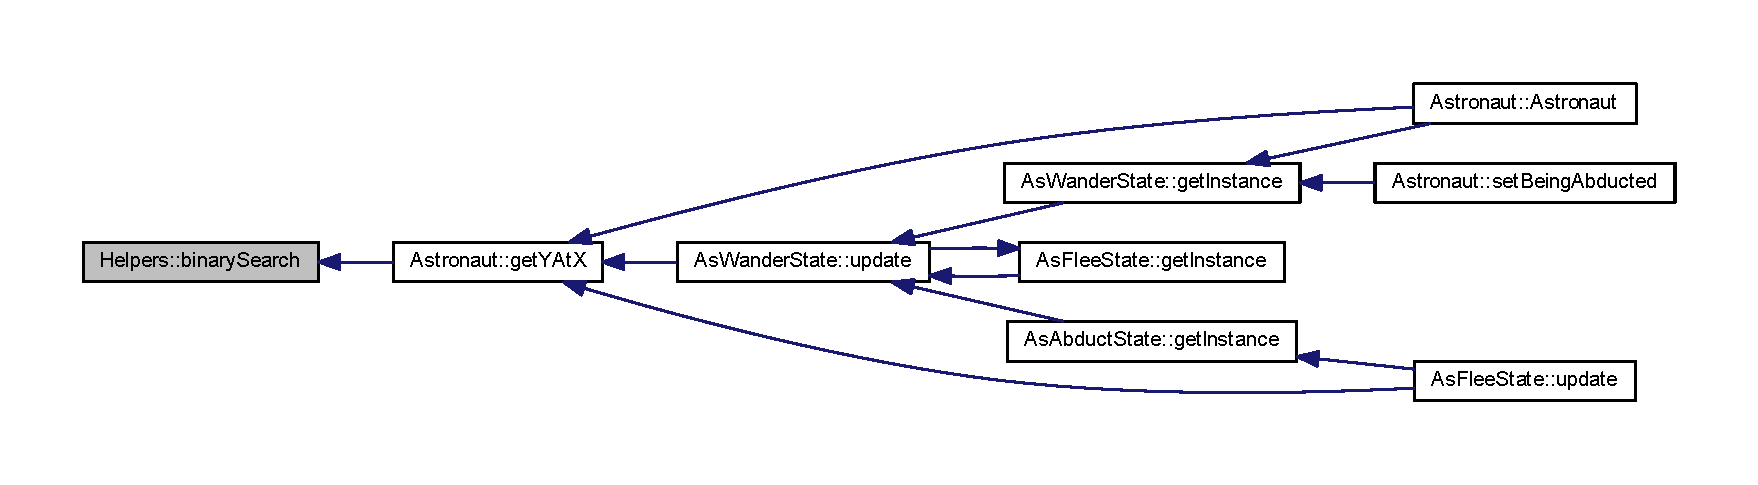
\includegraphics[width=350pt]{namespace_helpers_a17de449489ff14414634beaa710176cd_icgraph}
\end{center}
\end{figure}
\mbox{\Hypertarget{namespace_helpers_acafe0d99760ee8ee1ffbd365f974cafe}\label{namespace_helpers_acafe0d99760ee8ee1ffbd365f974cafe}} 
\index{Helpers@{Helpers}!clamp@{clamp}}
\index{clamp@{clamp}!Helpers@{Helpers}}
\subsubsection{\texorpdfstring{clamp()}{clamp()}}
{\footnotesize\ttfamily int Helpers\+::clamp (\begin{DoxyParamCaption}\item[{int}]{value,  }\item[{int}]{min,  }\item[{int}]{max }\end{DoxyParamCaption})\hspace{0.3cm}{\ttfamily [inline]}}

Here is the caller graph for this function\+:
\nopagebreak
\begin{figure}[H]
\begin{center}
\leavevmode
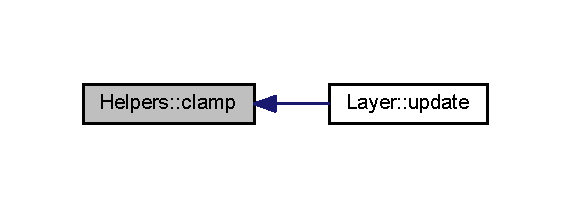
\includegraphics[width=274pt]{namespace_helpers_acafe0d99760ee8ee1ffbd365f974cafe_icgraph}
\end{center}
\end{figure}
\mbox{\Hypertarget{namespace_helpers_aad7d5773a24a3413ca8eca68aa6a872b}\label{namespace_helpers_aad7d5773a24a3413ca8eca68aa6a872b}} 
\index{Helpers@{Helpers}!get\+Length@{get\+Length}}
\index{get\+Length@{get\+Length}!Helpers@{Helpers}}
\subsubsection{\texorpdfstring{get\+Length()}{getLength()}}
{\footnotesize\ttfamily float Helpers\+::get\+Length (\begin{DoxyParamCaption}\item[{const sf\+::\+Vector2f \&}]{v }\end{DoxyParamCaption})\hspace{0.3cm}{\ttfamily [inline]}}

Here is the caller graph for this function\+:
\nopagebreak
\begin{figure}[H]
\begin{center}
\leavevmode
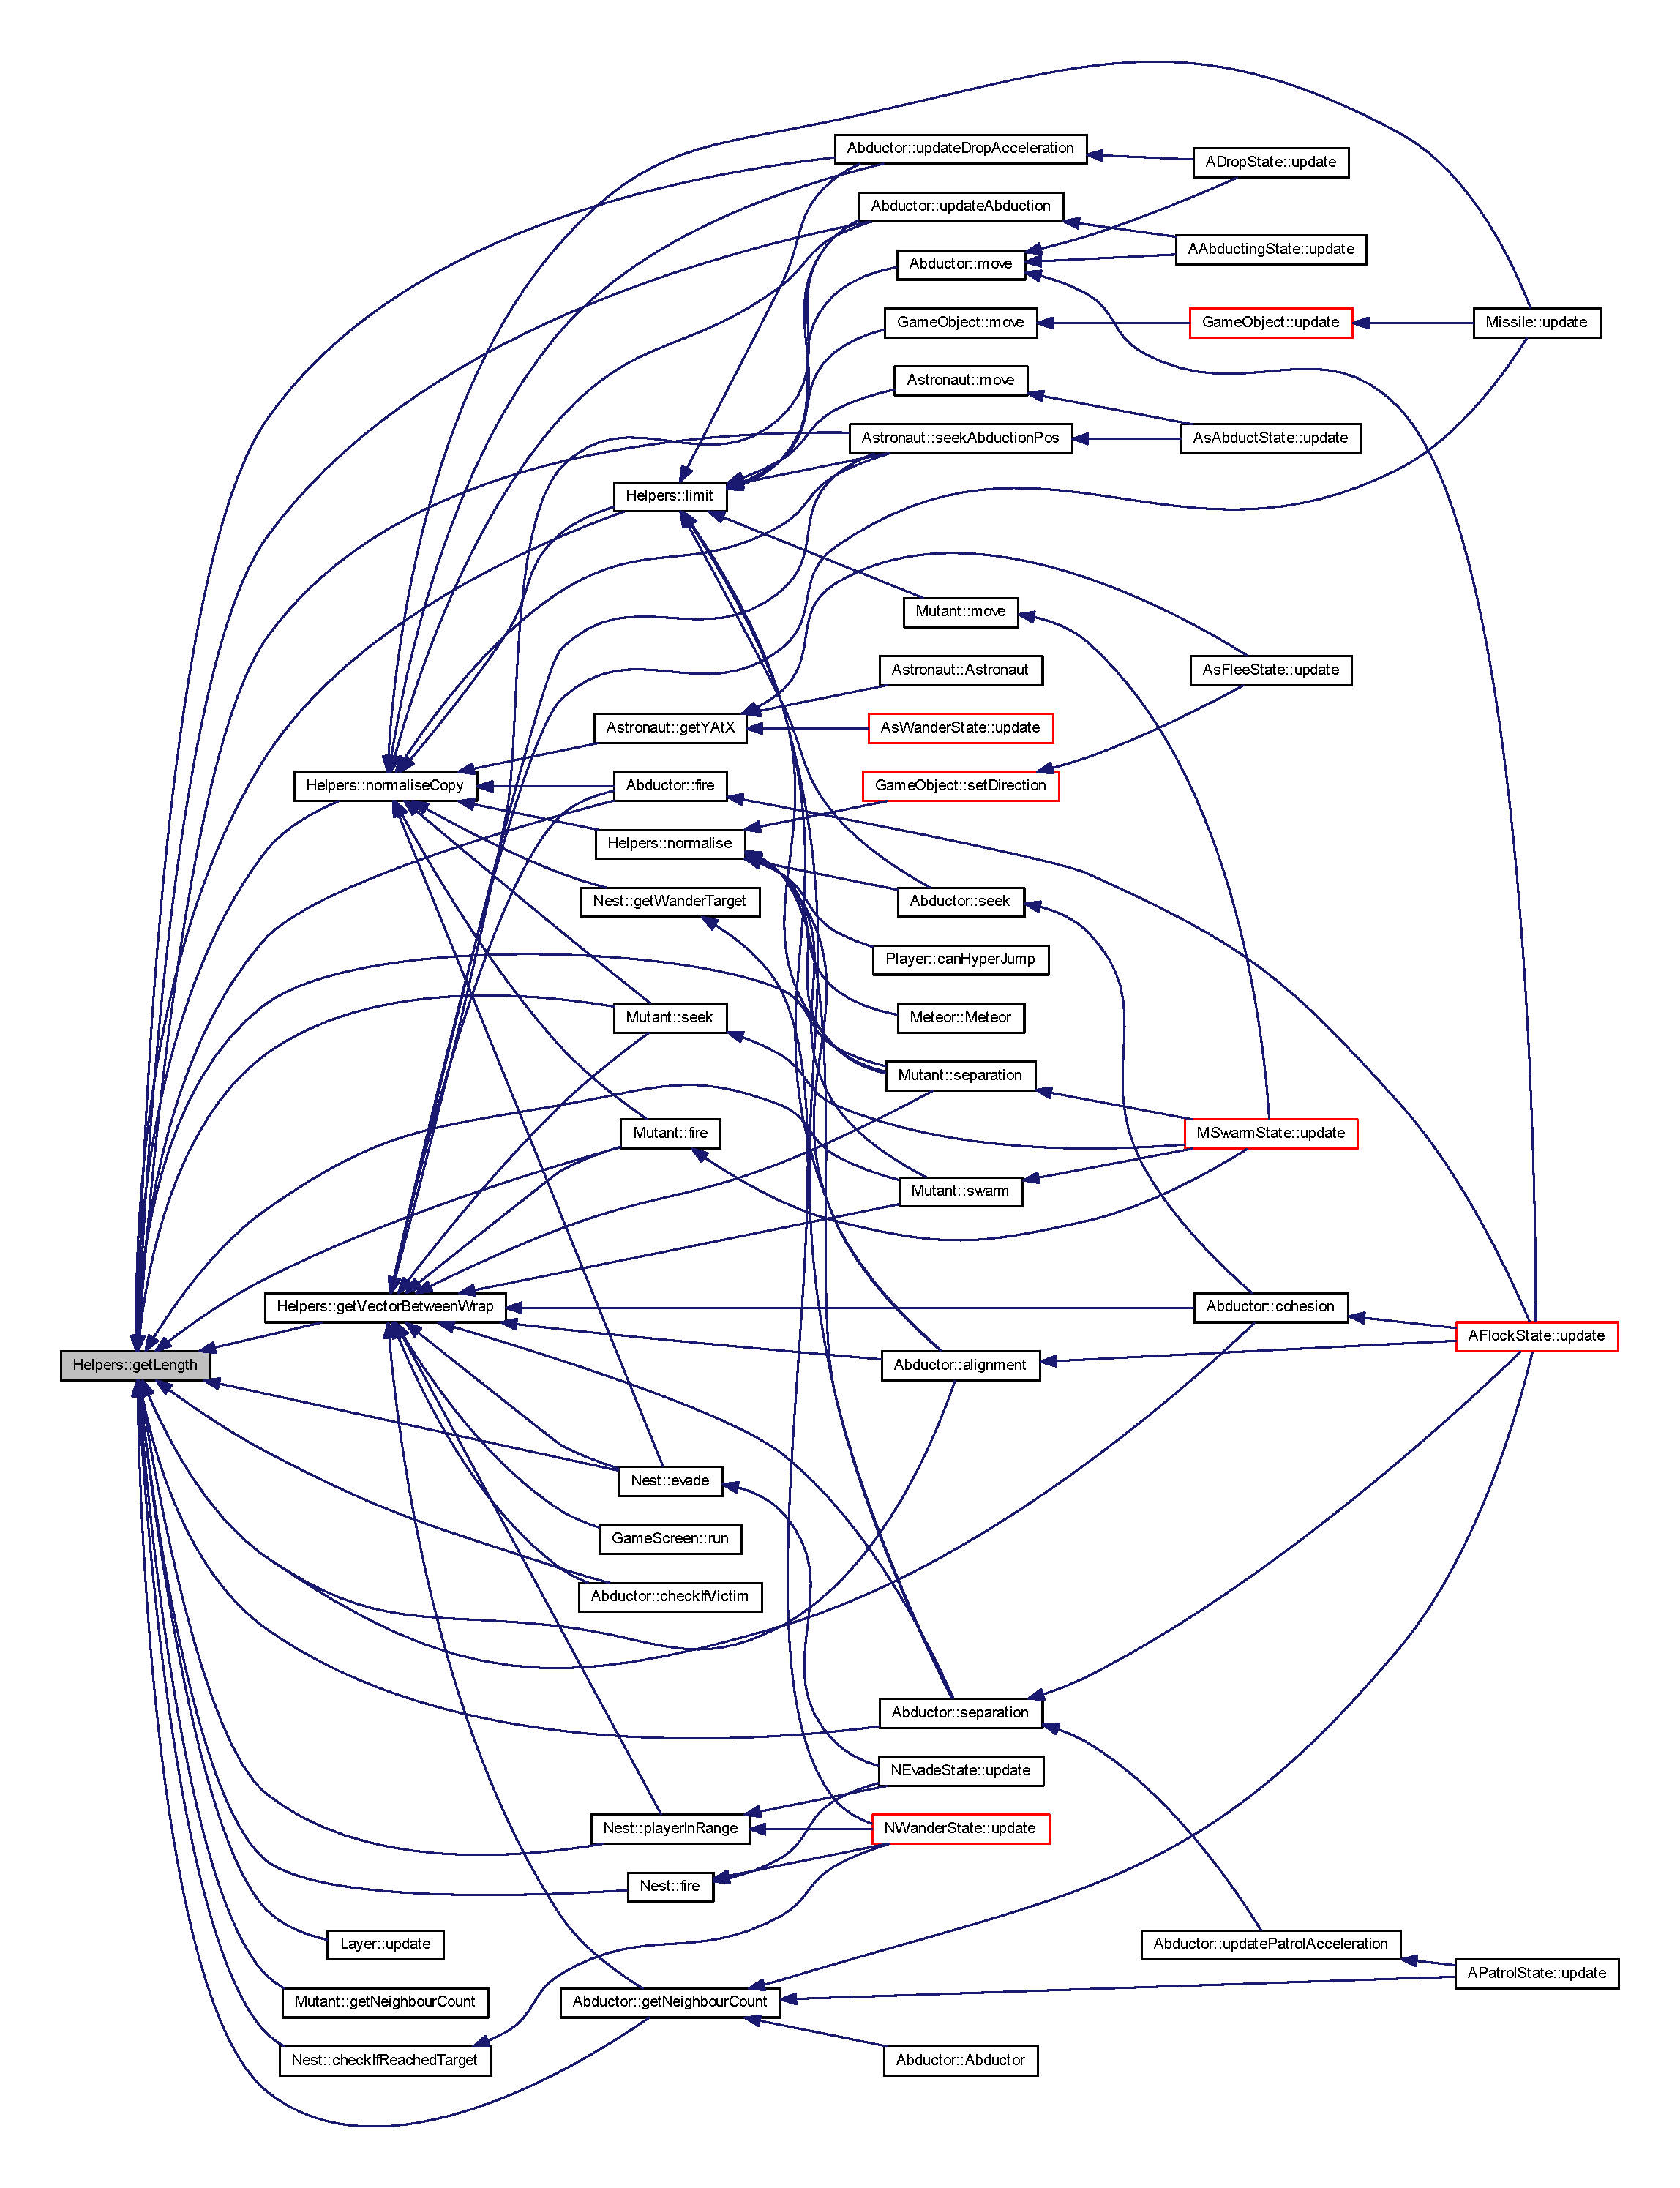
\includegraphics[width=350pt]{namespace_helpers_aad7d5773a24a3413ca8eca68aa6a872b_icgraph}
\end{center}
\end{figure}
\mbox{\Hypertarget{namespace_helpers_a93defc4f62a0b29303b84ea17eeeb2fb}\label{namespace_helpers_a93defc4f62a0b29303b84ea17eeeb2fb}} 
\index{Helpers@{Helpers}!get\+Vector\+Between\+Wrap@{get\+Vector\+Between\+Wrap}}
\index{get\+Vector\+Between\+Wrap@{get\+Vector\+Between\+Wrap}!Helpers@{Helpers}}
\subsubsection{\texorpdfstring{get\+Vector\+Between\+Wrap()}{getVectorBetweenWrap()}}
{\footnotesize\ttfamily sf\+::\+Vector2f Helpers\+::get\+Vector\+Between\+Wrap (\begin{DoxyParamCaption}\item[{const sf\+::\+Vector2f \&}]{world\+Size,  }\item[{const sf\+::\+Vector2f \&}]{position,  }\item[{const sf\+::\+Vector2f \&}]{target }\end{DoxyParamCaption})\hspace{0.3cm}{\ttfamily [inline]}}

Here is the call graph for this function\+:
\nopagebreak
\begin{figure}[H]
\begin{center}
\leavevmode
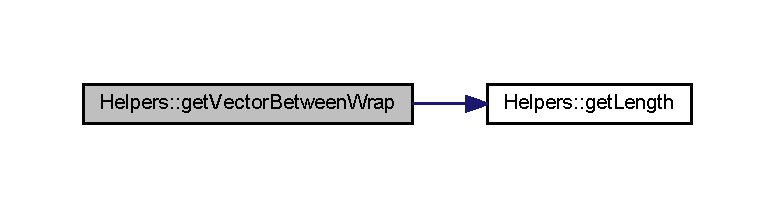
\includegraphics[width=350pt]{namespace_helpers_a93defc4f62a0b29303b84ea17eeeb2fb_cgraph}
\end{center}
\end{figure}
Here is the caller graph for this function\+:
\nopagebreak
\begin{figure}[H]
\begin{center}
\leavevmode
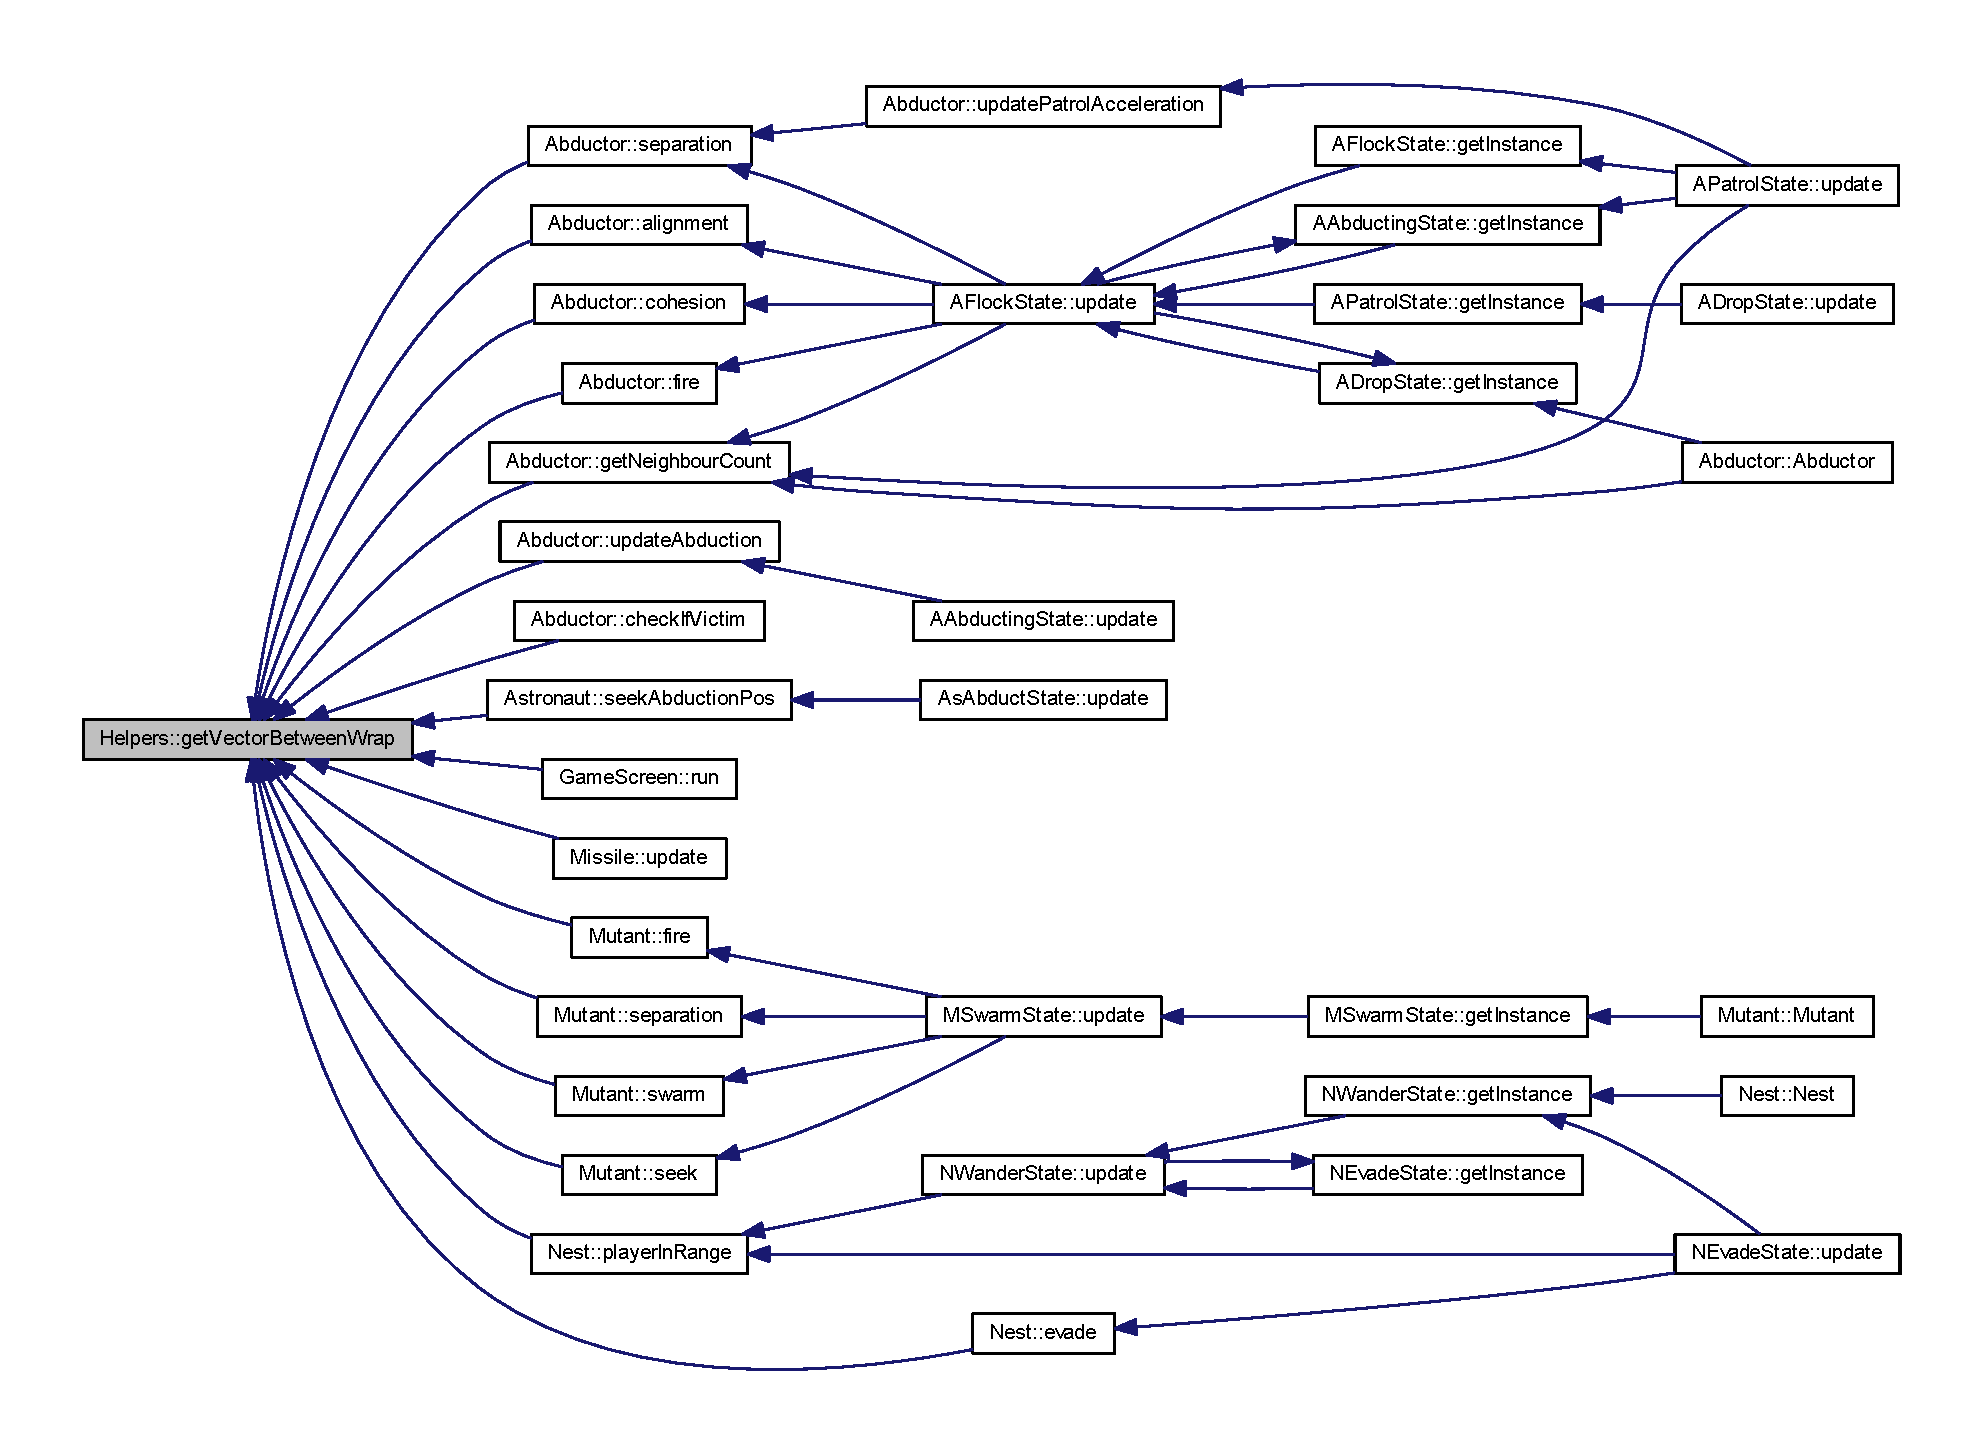
\includegraphics[width=350pt]{namespace_helpers_a93defc4f62a0b29303b84ea17eeeb2fb_icgraph}
\end{center}
\end{figure}
\mbox{\Hypertarget{namespace_helpers_a7b90b08e0cd27e52500271b582f8797b}\label{namespace_helpers_a7b90b08e0cd27e52500271b582f8797b}} 
\index{Helpers@{Helpers}!limit@{limit}}
\index{limit@{limit}!Helpers@{Helpers}}
\subsubsection{\texorpdfstring{limit()}{limit()}}
{\footnotesize\ttfamily void Helpers\+::limit (\begin{DoxyParamCaption}\item[{sf\+::\+Vector2f \&}]{v,  }\item[{float}]{max }\end{DoxyParamCaption})\hspace{0.3cm}{\ttfamily [inline]}}

Here is the call graph for this function\+:
\nopagebreak
\begin{figure}[H]
\begin{center}
\leavevmode
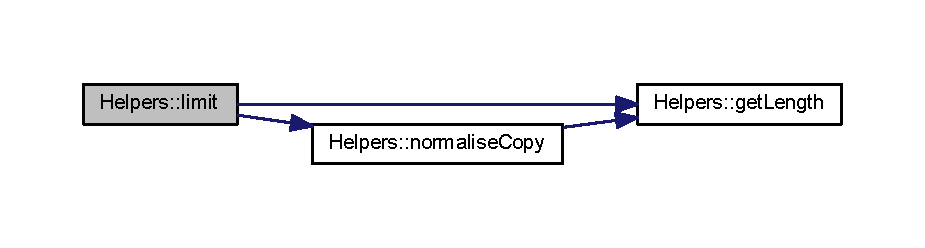
\includegraphics[width=350pt]{namespace_helpers_a7b90b08e0cd27e52500271b582f8797b_cgraph}
\end{center}
\end{figure}
Here is the caller graph for this function\+:
\nopagebreak
\begin{figure}[H]
\begin{center}
\leavevmode
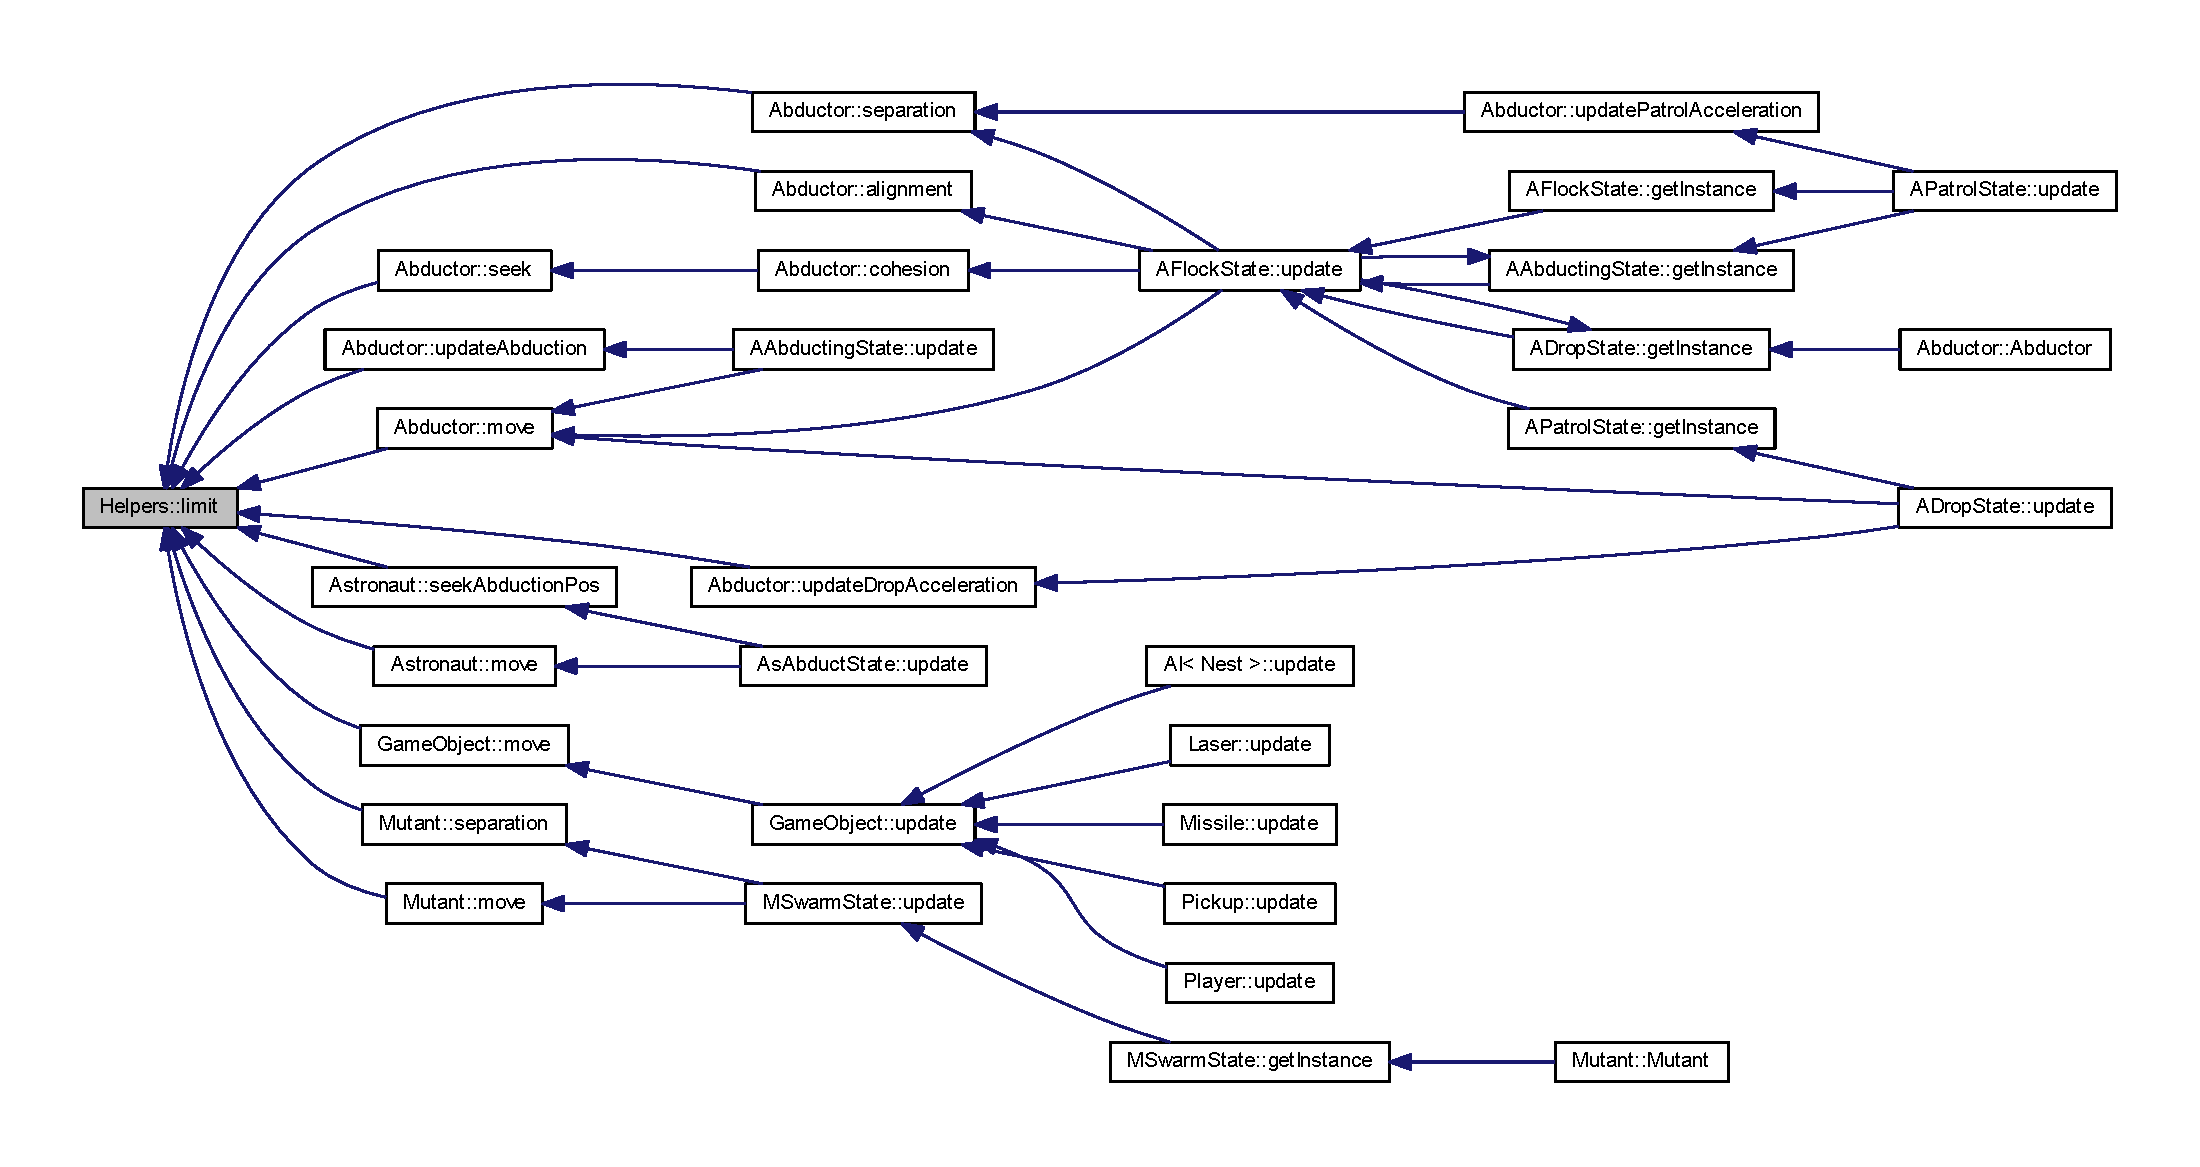
\includegraphics[width=350pt]{namespace_helpers_a7b90b08e0cd27e52500271b582f8797b_icgraph}
\end{center}
\end{figure}
\mbox{\Hypertarget{namespace_helpers_acf3ecf44a1d56b27ec102715bae903c1}\label{namespace_helpers_acf3ecf44a1d56b27ec102715bae903c1}} 
\index{Helpers@{Helpers}!normalise@{normalise}}
\index{normalise@{normalise}!Helpers@{Helpers}}
\subsubsection{\texorpdfstring{normalise()}{normalise()}}
{\footnotesize\ttfamily void Helpers\+::normalise (\begin{DoxyParamCaption}\item[{sf\+::\+Vector2f \&}]{v }\end{DoxyParamCaption})\hspace{0.3cm}{\ttfamily [inline]}}

Here is the call graph for this function\+:
\nopagebreak
\begin{figure}[H]
\begin{center}
\leavevmode
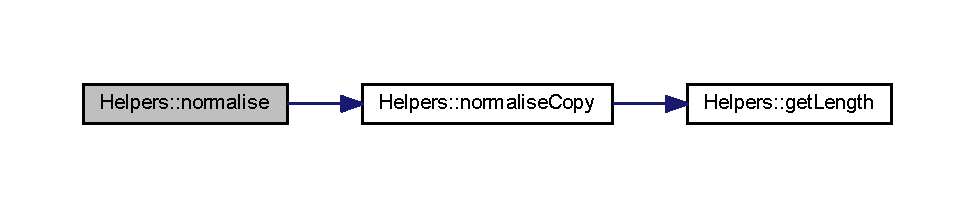
\includegraphics[width=350pt]{namespace_helpers_acf3ecf44a1d56b27ec102715bae903c1_cgraph}
\end{center}
\end{figure}
Here is the caller graph for this function\+:
\nopagebreak
\begin{figure}[H]
\begin{center}
\leavevmode
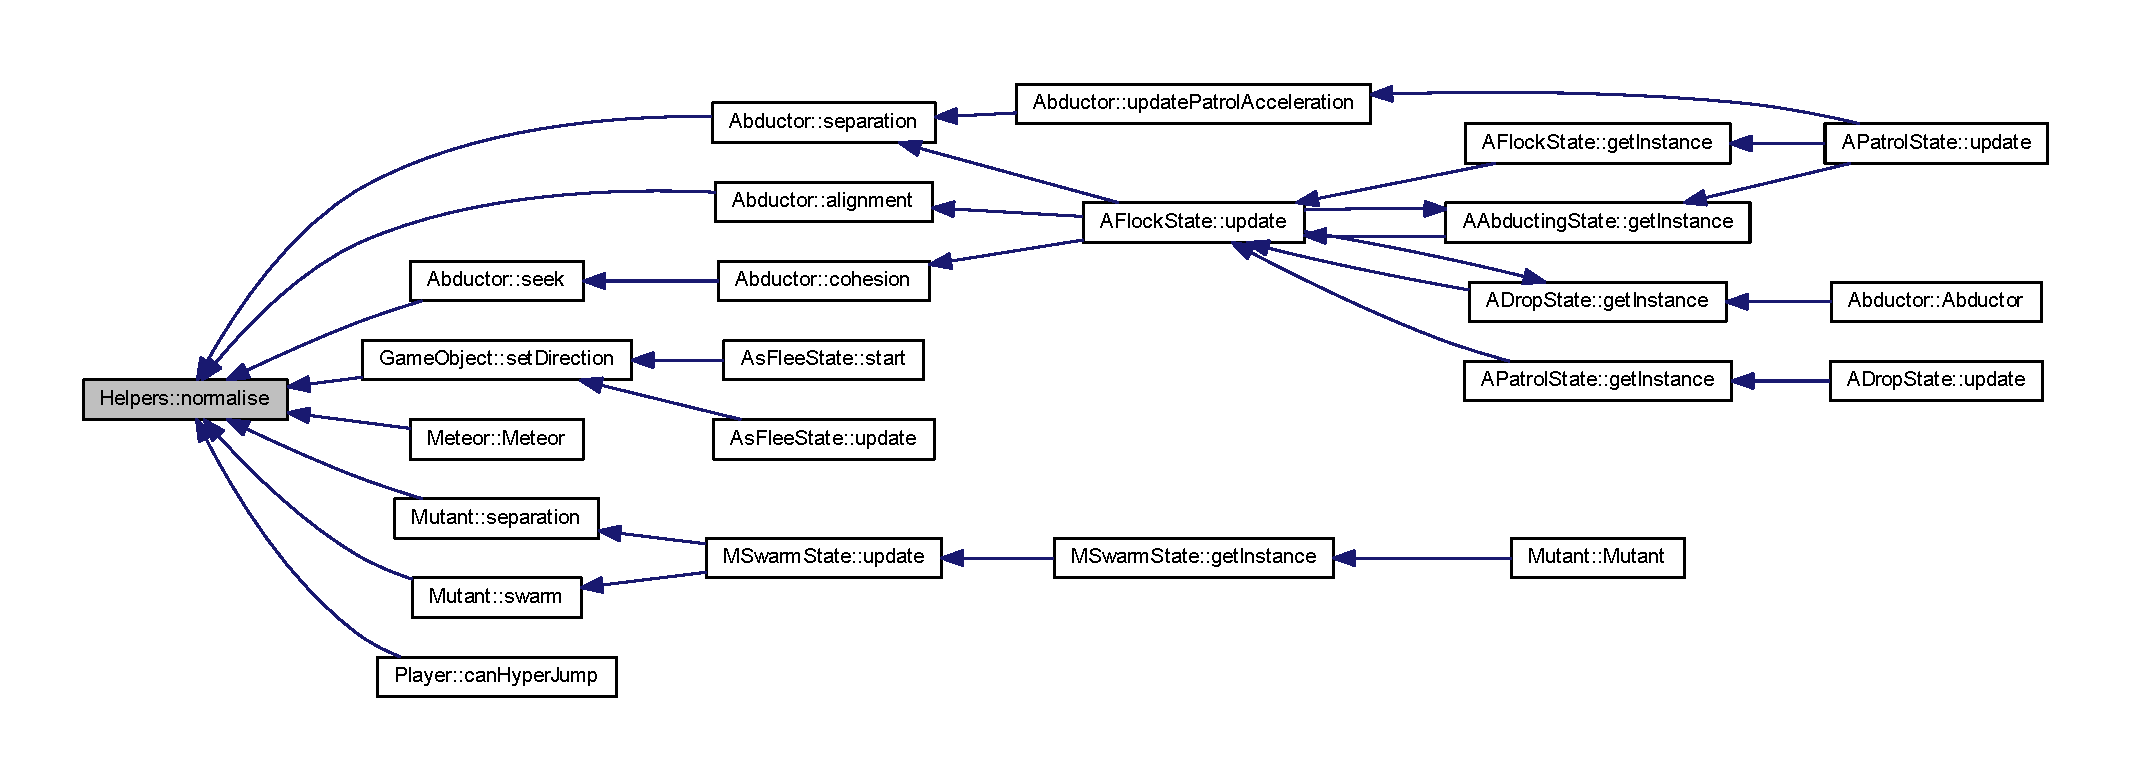
\includegraphics[width=350pt]{namespace_helpers_acf3ecf44a1d56b27ec102715bae903c1_icgraph}
\end{center}
\end{figure}
\mbox{\Hypertarget{namespace_helpers_a1c0a40432177c275488a904ea94eda66}\label{namespace_helpers_a1c0a40432177c275488a904ea94eda66}} 
\index{Helpers@{Helpers}!normalise\+Copy@{normalise\+Copy}}
\index{normalise\+Copy@{normalise\+Copy}!Helpers@{Helpers}}
\subsubsection{\texorpdfstring{normalise\+Copy()}{normaliseCopy()}}
{\footnotesize\ttfamily sf\+::\+Vector2f Helpers\+::normalise\+Copy (\begin{DoxyParamCaption}\item[{const sf\+::\+Vector2f \&}]{v }\end{DoxyParamCaption})\hspace{0.3cm}{\ttfamily [inline]}}

Here is the call graph for this function\+:
\nopagebreak
\begin{figure}[H]
\begin{center}
\leavevmode
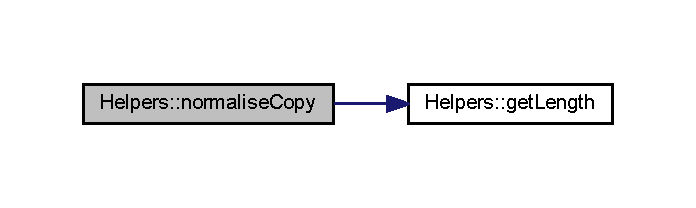
\includegraphics[width=334pt]{namespace_helpers_a1c0a40432177c275488a904ea94eda66_cgraph}
\end{center}
\end{figure}
Here is the caller graph for this function\+:
\nopagebreak
\begin{figure}[H]
\begin{center}
\leavevmode
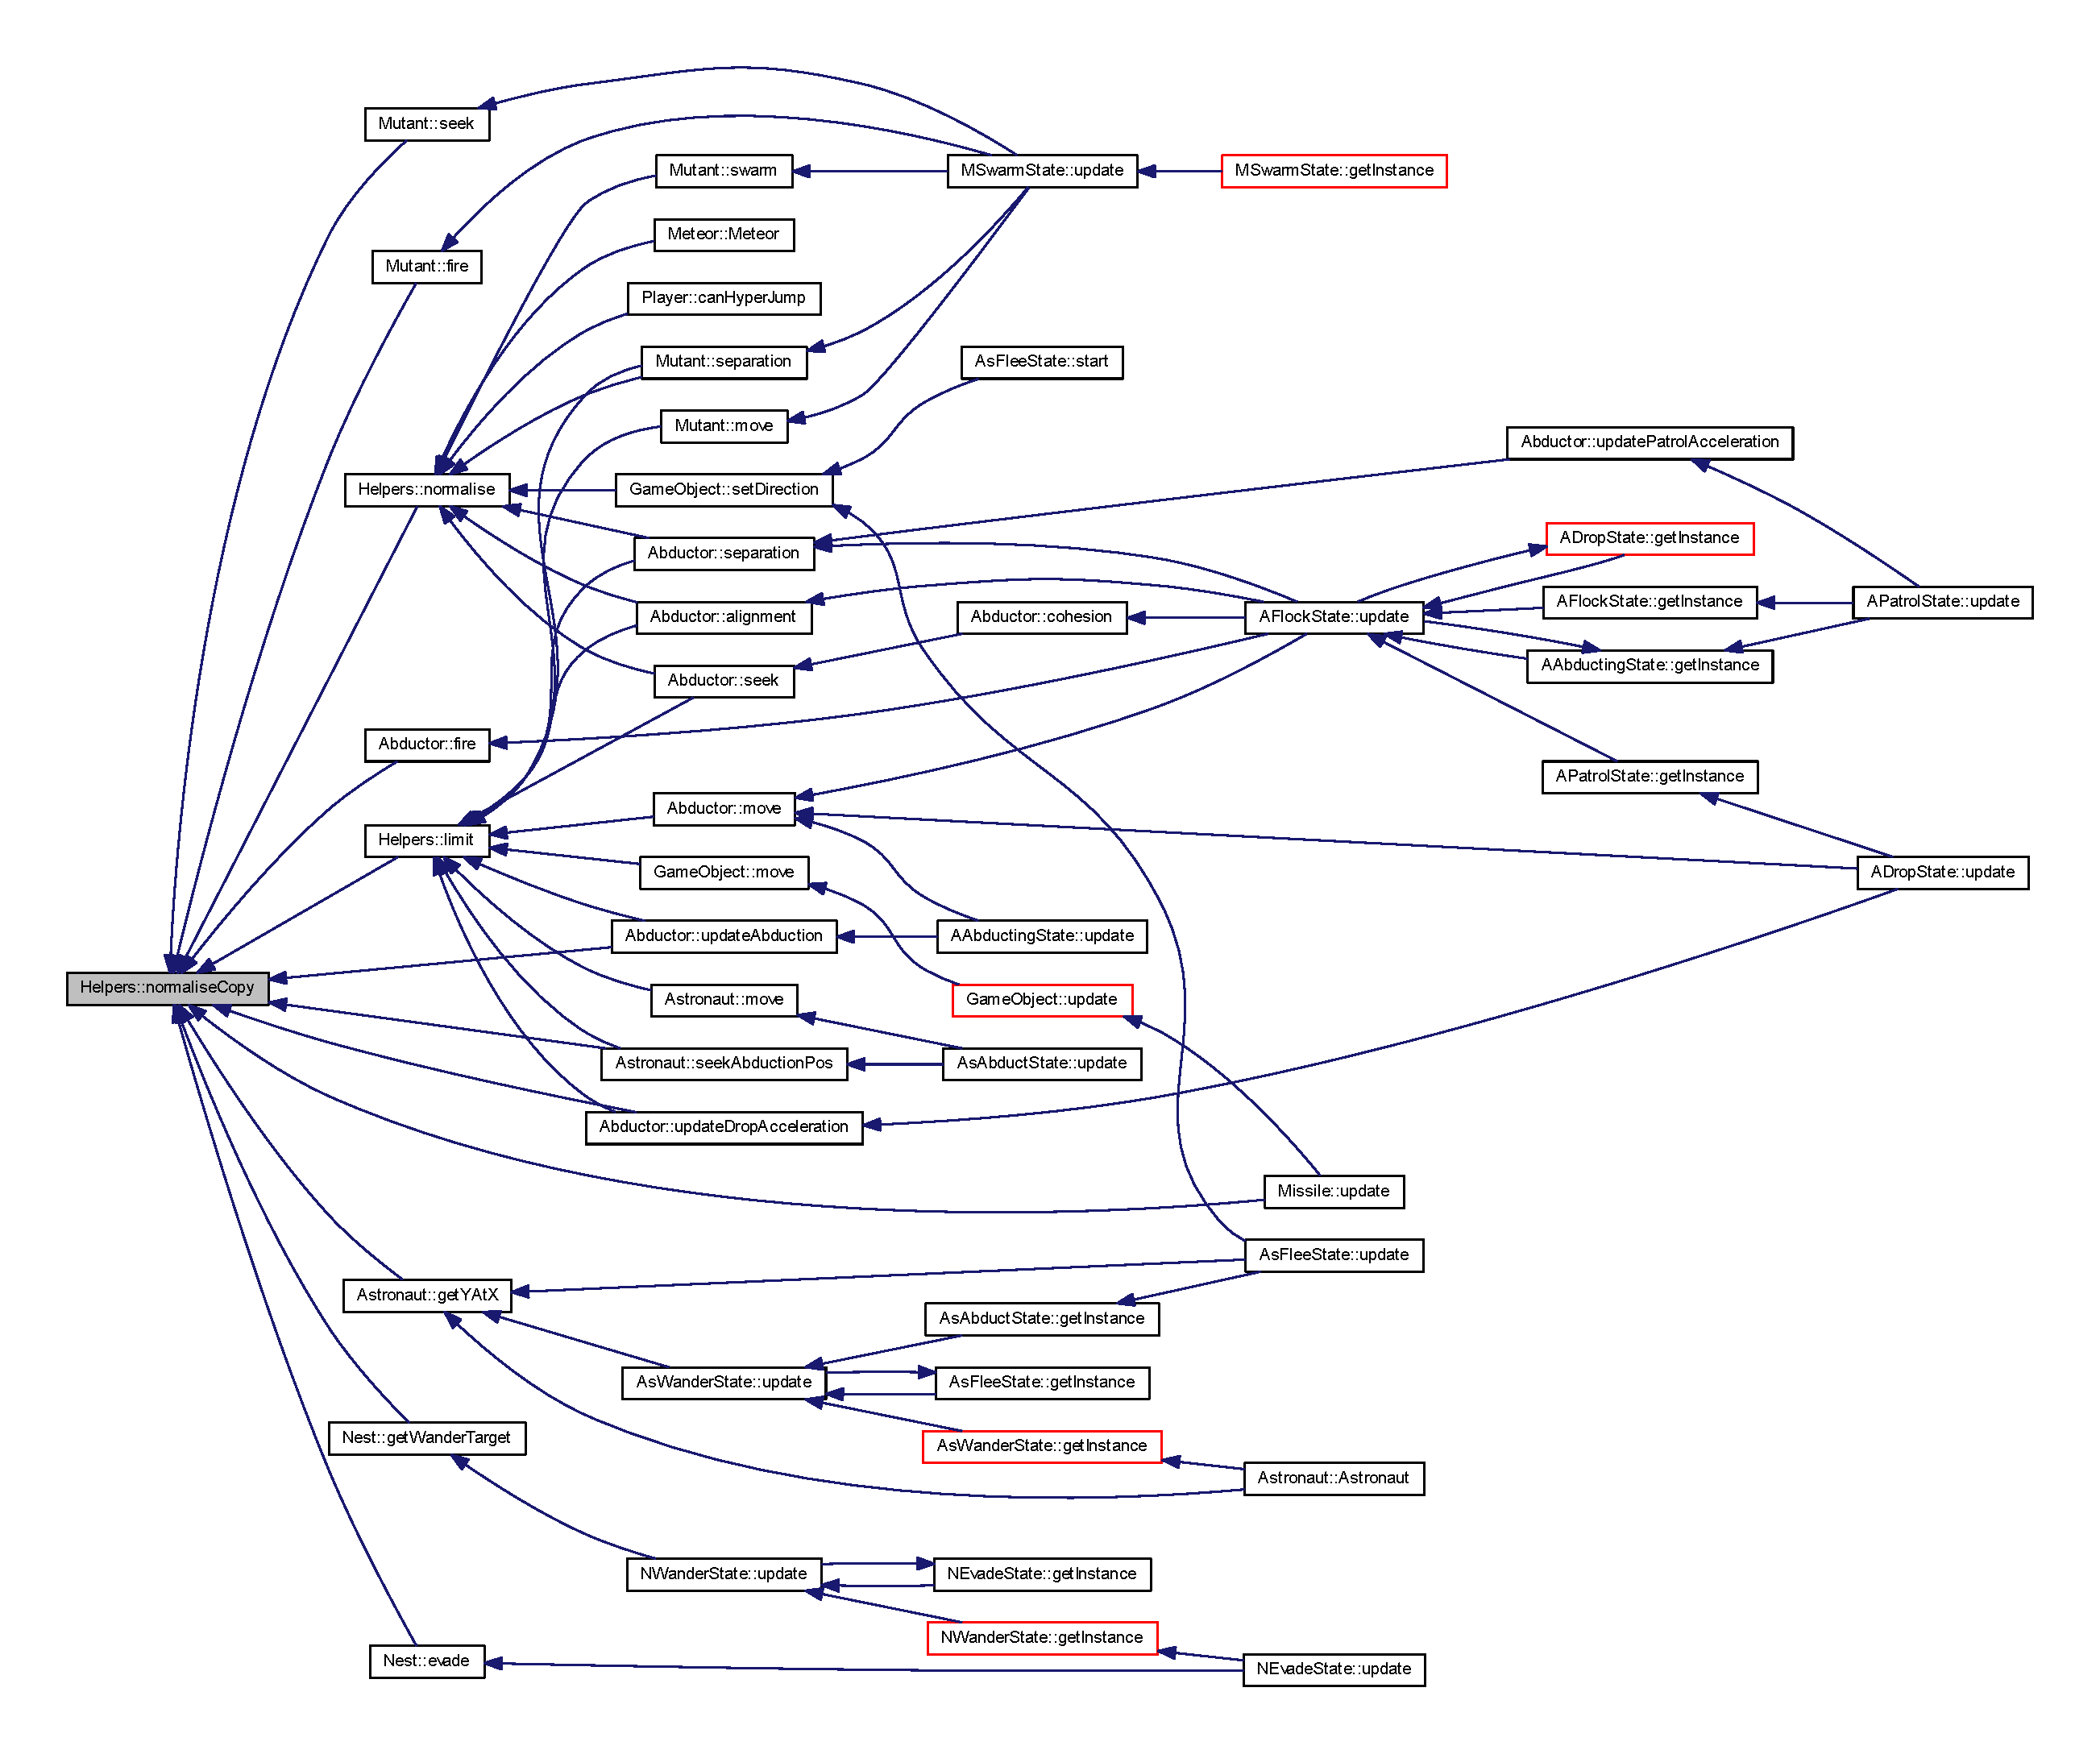
\includegraphics[width=350pt]{namespace_helpers_a1c0a40432177c275488a904ea94eda66_icgraph}
\end{center}
\end{figure}
\mbox{\Hypertarget{namespace_helpers_af4d3e03c8af50c930d3164b155f02e98}\label{namespace_helpers_af4d3e03c8af50c930d3164b155f02e98}} 
\index{Helpers@{Helpers}!random\+Number@{random\+Number}}
\index{random\+Number@{random\+Number}!Helpers@{Helpers}}
\subsubsection{\texorpdfstring{random\+Number()}{randomNumber()}}
{\footnotesize\ttfamily int Helpers\+::random\+Number (\begin{DoxyParamCaption}\item[{int}]{min,  }\item[{int}]{max }\end{DoxyParamCaption})\hspace{0.3cm}{\ttfamily [inline]}}

Here is the caller graph for this function\+:
\nopagebreak
\begin{figure}[H]
\begin{center}
\leavevmode
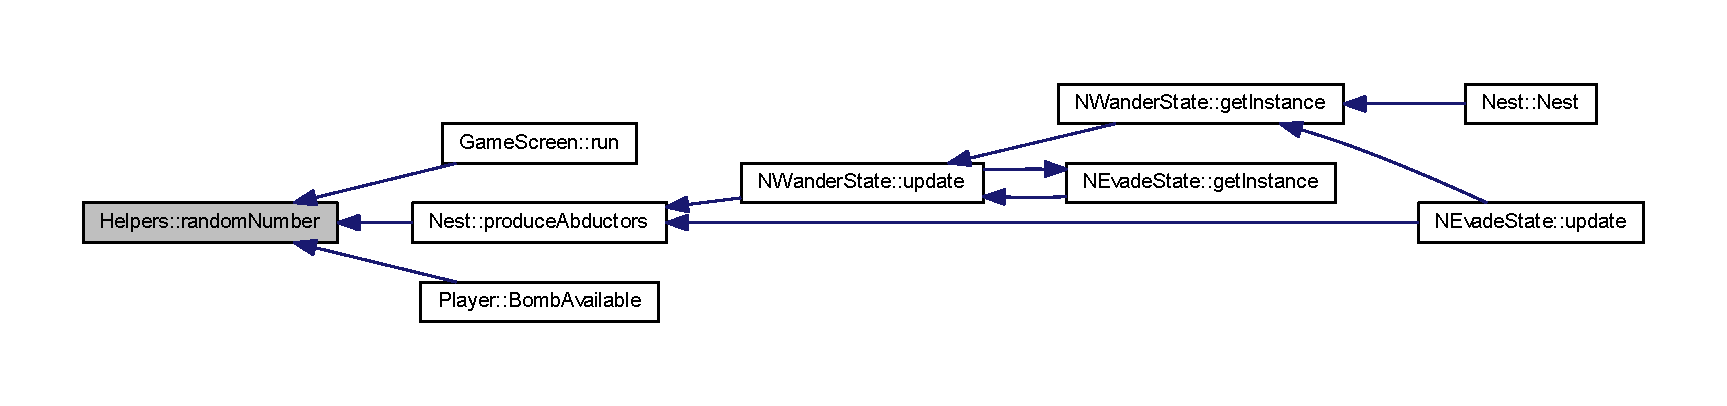
\includegraphics[width=350pt]{namespace_helpers_af4d3e03c8af50c930d3164b155f02e98_icgraph}
\end{center}
\end{figure}
\mbox{\Hypertarget{namespace_helpers_ad1aef5710c67da43b9bbed2107c1e11b}\label{namespace_helpers_ad1aef5710c67da43b9bbed2107c1e11b}} 
\index{Helpers@{Helpers}!random\+NumberF@{random\+NumberF}}
\index{random\+NumberF@{random\+NumberF}!Helpers@{Helpers}}
\subsubsection{\texorpdfstring{random\+Number\+F()}{randomNumberF()}}
{\footnotesize\ttfamily float Helpers\+::random\+NumberF (\begin{DoxyParamCaption}\item[{float}]{min,  }\item[{float}]{max }\end{DoxyParamCaption})\hspace{0.3cm}{\ttfamily [inline]}}

Here is the caller graph for this function\+:
\nopagebreak
\begin{figure}[H]
\begin{center}
\leavevmode
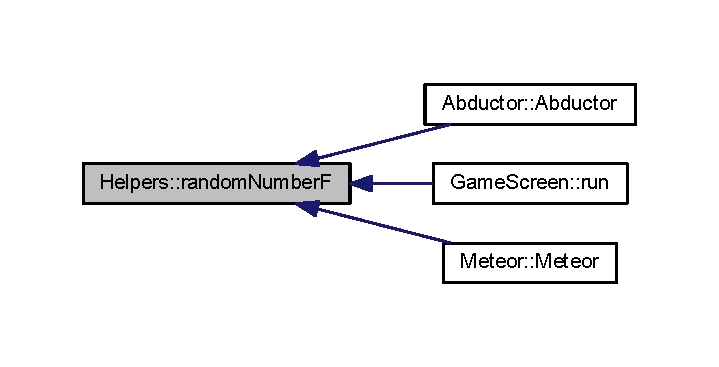
\includegraphics[width=345pt]{namespace_helpers_ad1aef5710c67da43b9bbed2107c1e11b_icgraph}
\end{center}
\end{figure}

\chapter{Class Documentation}
\hypertarget{class_a_abducting_state}{}\section{A\+Abducting\+State Class Reference}
\label{class_a_abducting_state}\index{A\+Abducting\+State@{A\+Abducting\+State}}


{\ttfamily \#include $<$Abductor\+States.\+h$>$}



Inheritance diagram for A\+Abducting\+State\+:\nopagebreak
\begin{figure}[H]
\begin{center}
\leavevmode
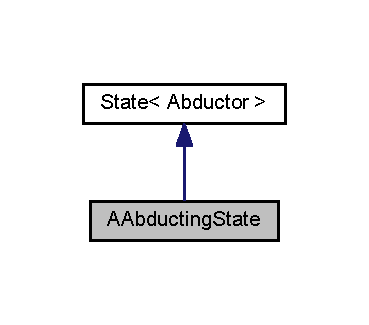
\includegraphics[width=177pt]{class_a_abducting_state__inherit__graph}
\end{center}
\end{figure}


Collaboration diagram for A\+Abducting\+State\+:\nopagebreak
\begin{figure}[H]
\begin{center}
\leavevmode
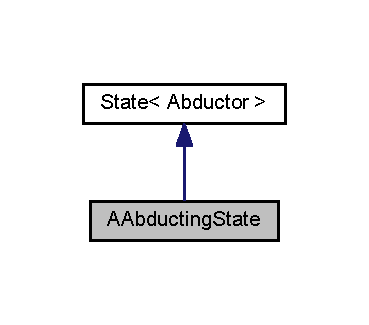
\includegraphics[width=177pt]{class_a_abducting_state__coll__graph}
\end{center}
\end{figure}
\subsection*{Public Member Functions}
\begin{DoxyCompactItemize}
\item 
void \hyperlink{class_a_abducting_state_a4a592efc0ae90b3c88de9cb676ed8357}{start} (\hyperlink{class_abductor}{Abductor} $\ast$) override
\item 
void \hyperlink{class_a_abducting_state_a37963b87c9c9fea8cfc8252618a53c98}{update} (\hyperlink{class_abductor}{Abductor} $\ast$, float) override
\item 
void \hyperlink{class_a_abducting_state_a618a6c11d2dc823b11161ff3a0c88ef8}{end} (\hyperlink{class_abductor}{Abductor} $\ast$) override
\end{DoxyCompactItemize}
\subsection*{Static Public Member Functions}
\begin{DoxyCompactItemize}
\item 
static std\+::shared\+\_\+ptr$<$ \hyperlink{class_a_abducting_state}{A\+Abducting\+State} $>$ \& \hyperlink{class_a_abducting_state_a0843d5645fe863959f454a9497cc32ab}{get\+Instance} ()
\end{DoxyCompactItemize}
\subsection*{Additional Inherited Members}


\subsection{Member Function Documentation}
\mbox{\Hypertarget{class_a_abducting_state_a618a6c11d2dc823b11161ff3a0c88ef8}\label{class_a_abducting_state_a618a6c11d2dc823b11161ff3a0c88ef8}} 
\index{A\+Abducting\+State@{A\+Abducting\+State}!end@{end}}
\index{end@{end}!A\+Abducting\+State@{A\+Abducting\+State}}
\subsubsection{\texorpdfstring{end()}{end()}}
{\footnotesize\ttfamily void A\+Abducting\+State\+::end (\begin{DoxyParamCaption}\item[{\hyperlink{class_abductor}{Abductor} $\ast$}]{abductor }\end{DoxyParamCaption})\hspace{0.3cm}{\ttfamily [override]}, {\ttfamily [virtual]}}



Implements \hyperlink{class_state_a97d058722f988c008e912a0e5ec879b3}{State$<$ Abductor $>$}.

\mbox{\Hypertarget{class_a_abducting_state_a0843d5645fe863959f454a9497cc32ab}\label{class_a_abducting_state_a0843d5645fe863959f454a9497cc32ab}} 
\index{A\+Abducting\+State@{A\+Abducting\+State}!get\+Instance@{get\+Instance}}
\index{get\+Instance@{get\+Instance}!A\+Abducting\+State@{A\+Abducting\+State}}
\subsubsection{\texorpdfstring{get\+Instance()}{getInstance()}}
{\footnotesize\ttfamily static std\+::shared\+\_\+ptr$<$\hyperlink{class_a_abducting_state}{A\+Abducting\+State}$>$\& A\+Abducting\+State\+::get\+Instance (\begin{DoxyParamCaption}{ }\end{DoxyParamCaption})\hspace{0.3cm}{\ttfamily [inline]}, {\ttfamily [static]}}

Here is the call graph for this function\+:
\nopagebreak
\begin{figure}[H]
\begin{center}
\leavevmode
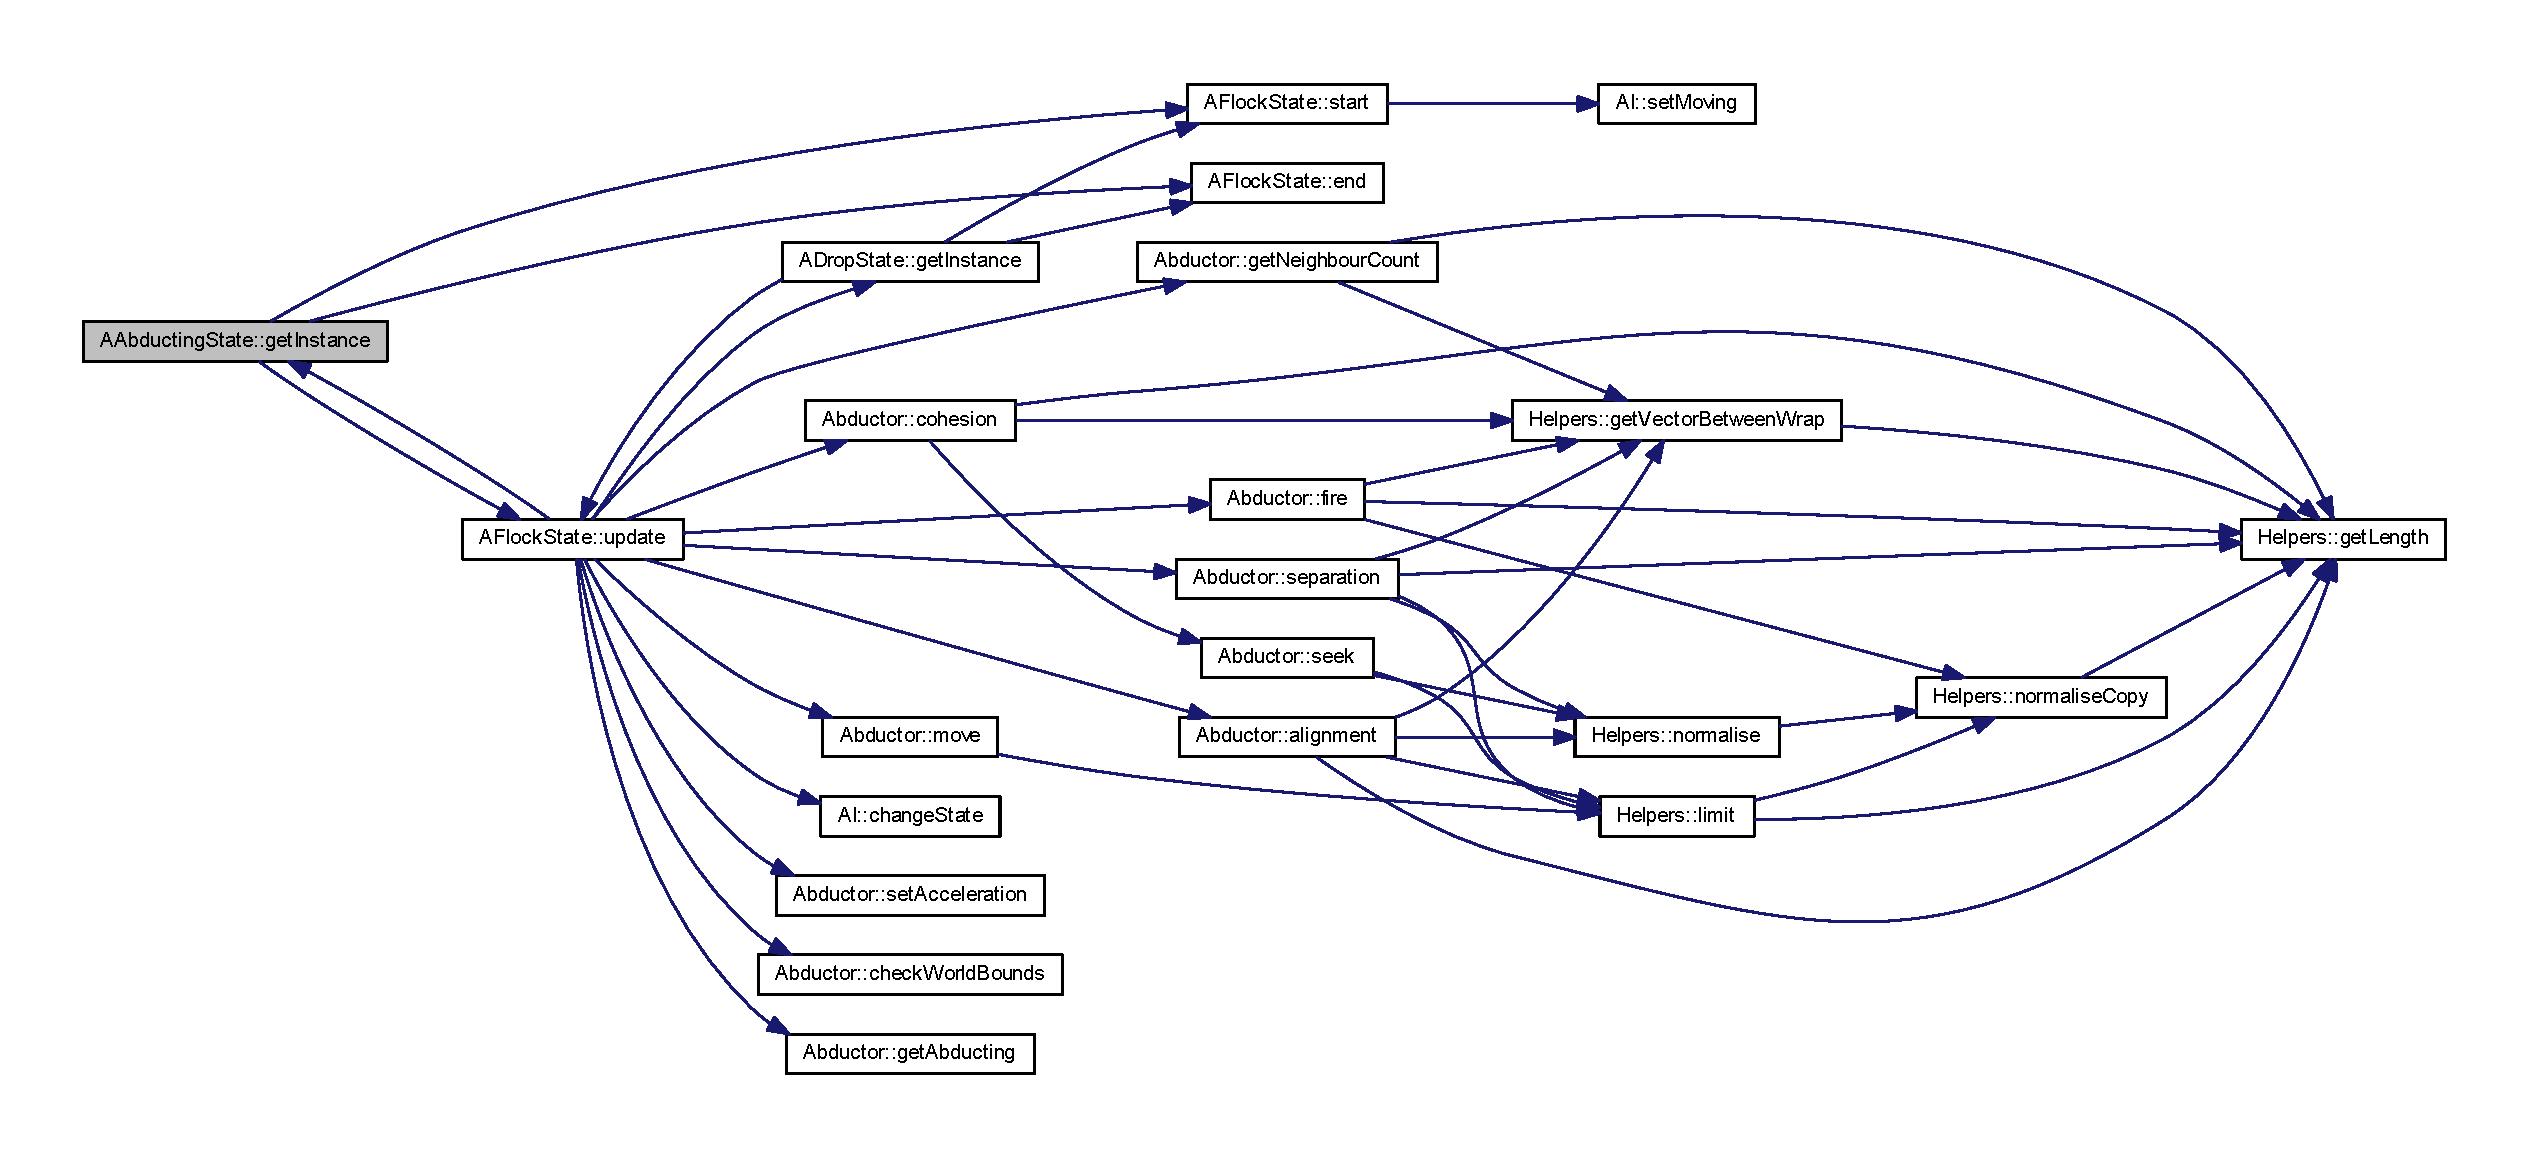
\includegraphics[width=350pt]{class_a_abducting_state_a0843d5645fe863959f454a9497cc32ab_cgraph}
\end{center}
\end{figure}
Here is the caller graph for this function\+:
\nopagebreak
\begin{figure}[H]
\begin{center}
\leavevmode
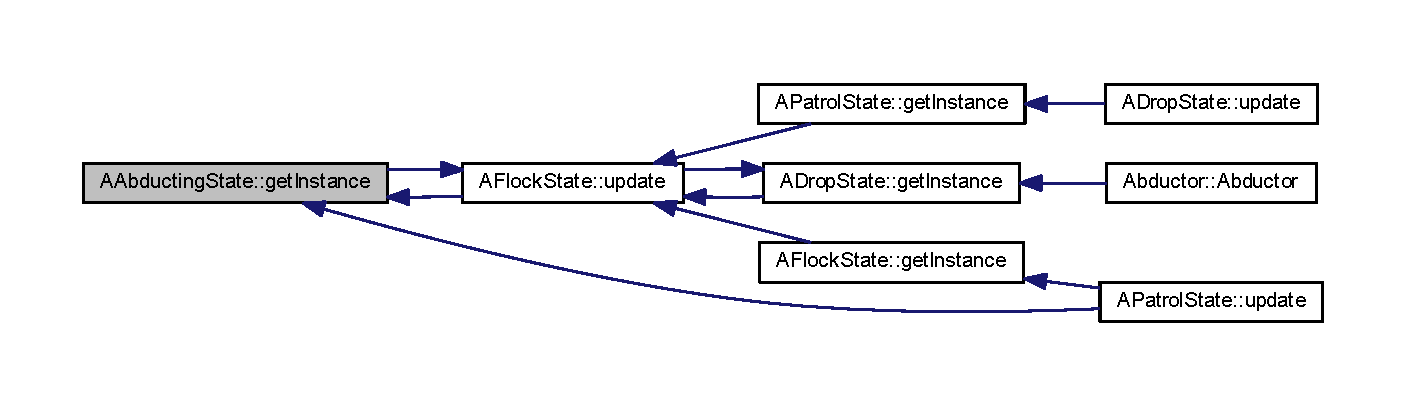
\includegraphics[width=350pt]{class_a_abducting_state_a0843d5645fe863959f454a9497cc32ab_icgraph}
\end{center}
\end{figure}
\mbox{\Hypertarget{class_a_abducting_state_a4a592efc0ae90b3c88de9cb676ed8357}\label{class_a_abducting_state_a4a592efc0ae90b3c88de9cb676ed8357}} 
\index{A\+Abducting\+State@{A\+Abducting\+State}!start@{start}}
\index{start@{start}!A\+Abducting\+State@{A\+Abducting\+State}}
\subsubsection{\texorpdfstring{start()}{start()}}
{\footnotesize\ttfamily void A\+Abducting\+State\+::start (\begin{DoxyParamCaption}\item[{\hyperlink{class_abductor}{Abductor} $\ast$}]{abductor }\end{DoxyParamCaption})\hspace{0.3cm}{\ttfamily [override]}, {\ttfamily [virtual]}}



Implements \hyperlink{class_state_abc29d36b0462a306ac9b32f36571d783}{State$<$ Abductor $>$}.

Here is the call graph for this function\+:
\nopagebreak
\begin{figure}[H]
\begin{center}
\leavevmode
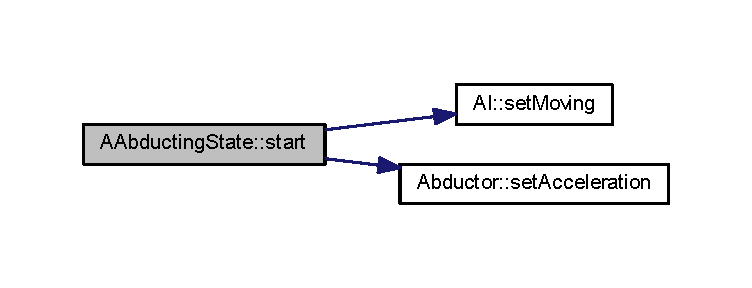
\includegraphics[width=350pt]{class_a_abducting_state_a4a592efc0ae90b3c88de9cb676ed8357_cgraph}
\end{center}
\end{figure}
\mbox{\Hypertarget{class_a_abducting_state_a37963b87c9c9fea8cfc8252618a53c98}\label{class_a_abducting_state_a37963b87c9c9fea8cfc8252618a53c98}} 
\index{A\+Abducting\+State@{A\+Abducting\+State}!update@{update}}
\index{update@{update}!A\+Abducting\+State@{A\+Abducting\+State}}
\subsubsection{\texorpdfstring{update()}{update()}}
{\footnotesize\ttfamily void A\+Abducting\+State\+::update (\begin{DoxyParamCaption}\item[{\hyperlink{class_abductor}{Abductor} $\ast$}]{abductor,  }\item[{float}]{dt }\end{DoxyParamCaption})\hspace{0.3cm}{\ttfamily [override]}, {\ttfamily [virtual]}}



Implements \hyperlink{class_state_a30b5f87ed3e3a05fafeaf898e43518ea}{State$<$ Abductor $>$}.

Here is the call graph for this function\+:
\nopagebreak
\begin{figure}[H]
\begin{center}
\leavevmode
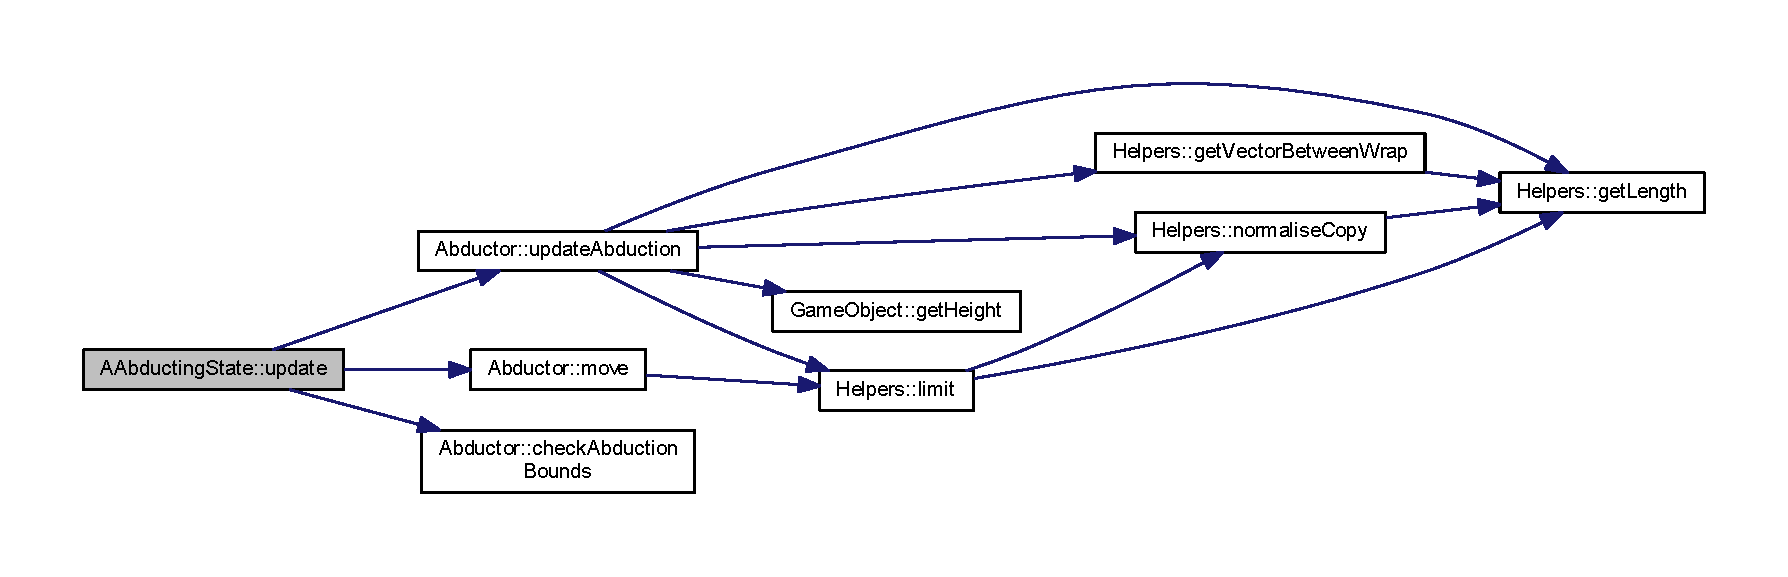
\includegraphics[width=350pt]{class_a_abducting_state_a37963b87c9c9fea8cfc8252618a53c98_cgraph}
\end{center}
\end{figure}


The documentation for this class was generated from the following files\+:\begin{DoxyCompactItemize}
\item 
include/\hyperlink{_abductor_states_8h}{Abductor\+States.\+h}\item 
src/\hyperlink{_abductor_states_8cpp}{Abductor\+States.\+cpp}\end{DoxyCompactItemize}

\hypertarget{class_abductor}{}\section{Abductor Class Reference}
\label{class_abductor}\index{Abductor@{Abductor}}


{\ttfamily \#include $<$Abductor.\+h$>$}



Inheritance diagram for Abductor\+:\nopagebreak
\begin{figure}[H]
\begin{center}
\leavevmode
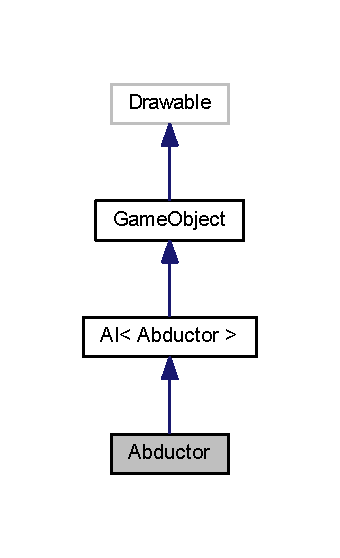
\includegraphics[width=163pt]{class_abductor__inherit__graph}
\end{center}
\end{figure}


Collaboration diagram for Abductor\+:\nopagebreak
\begin{figure}[H]
\begin{center}
\leavevmode
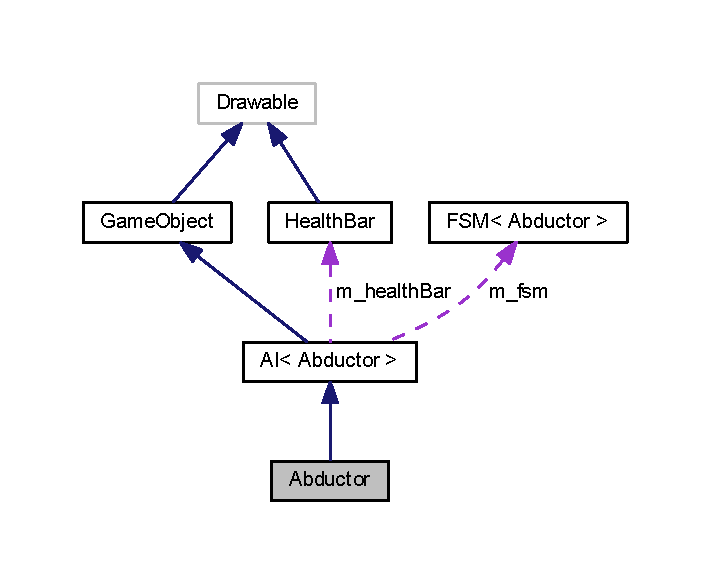
\includegraphics[width=341pt]{class_abductor__coll__graph}
\end{center}
\end{figure}
\subsection*{Public Types}
\begin{DoxyCompactItemize}
\item 
typedef std\+::vector$<$ std\+::shared\+\_\+ptr$<$ \hyperlink{class_game_object}{Game\+Object} $>$ $>$ \hyperlink{class_abductor_a2fc54e0ab08037996dd212d4d2d0443f}{Game\+Object\+Ptr\+Vector}
\item 
typedef std\+::unordered\+\_\+map$<$ std\+::string, \hyperlink{class_abductor_a2fc54e0ab08037996dd212d4d2d0443f}{Game\+Object\+Ptr\+Vector} $>$ \hyperlink{class_abductor_a15ce0d62a23ac0c3e335874ff4286f5f}{Game\+Object\+Map}
\end{DoxyCompactItemize}
\subsection*{Public Member Functions}
\begin{DoxyCompactItemize}
\item 
\hyperlink{class_abductor_ac68525ef8d05680afbef24761e2baa8c}{Abductor} (const sf\+::\+Vector2f \&start\+Pos, const sf\+::\+Vector2f \&world\+Size, std\+::shared\+\_\+ptr$<$ \hyperlink{class_game_object}{Game\+Object} $>$ player, \hyperlink{class_abductor_a15ce0d62a23ac0c3e335874ff4286f5f}{Game\+Object\+Map} \&game\+Objects\+Ref)
\item 
sf\+::\+Vector2f \hyperlink{class_abductor_aac2bef46d63d3aa630a34ee1cb23a7f6}{separation} ()
\item 
sf\+::\+Vector2f \hyperlink{class_abductor_ac8ef27110672980a395fa9ba68299337}{alignment} ()
\item 
sf\+::\+Vector2f \hyperlink{class_abductor_ad1660967efd5c4abcdee49989a966722}{cohesion} ()
\item 
sf\+::\+Vector2f \hyperlink{class_abductor_a2c5431c2d7afa37f9f083762eff5a995}{seek} (const sf\+::\+Vector2f \&v)
\item 
void \hyperlink{class_abductor_a7147793ce13d446f83eb52920dfa15f7}{set\+Acceleration} (const sf\+::\+Vector2f \&acceleration)
\item 
void \hyperlink{class_abductor_a10bb137ba1b1707466f0a893052a0b30}{move} (float dt) override
\item 
int \hyperlink{class_abductor_ae8c4cc87315ccc822d59d73a7c12c94a}{get\+Neighbour\+Count} () const
\item 
float \hyperlink{class_abductor_a8bc04ea46a52e8a58feceee69a8965d0}{get\+Force\+Amount} () const
\item 
void \hyperlink{class_abductor_aad7a615477ffe510984c8df16e98c903}{set\+Direction} (const sf\+::\+Vector2f \&dir)
\item 
sf\+::\+Vector2f \hyperlink{class_abductor_a30a40083cd604343d7b1d63e1a48a3fa}{get\+Direction} () const
\item 
void \hyperlink{class_abductor_aab823ab3fd94214f90b003661e036d03}{update\+Drop\+Acceleration} ()
\item 
void \hyperlink{class_abductor_a24cc63afd005eef7d1ed694933a2c2a0}{update\+Patrol\+Acceleration} ()
\item 
void \hyperlink{class_abductor_a12b84d9d38bec8ed3b495c5657903e50}{fire} (float dt)
\item 
bool \hyperlink{class_abductor_acc2841707aaeb5719ecc615b5fe6bf56}{reached\+Target} () const
\item 
void \hyperlink{class_abductor_a4b86fdcd63a060c53da22f092a113b24}{check\+World\+Bounds} () override
\item 
bool \hyperlink{class_abductor_ac0c62963a2e8bdac8c34bfb2a2c0b868}{get\+Abducting} () const
\item 
void \hyperlink{class_abductor_a1069f5de8e0696be938a741f4b931855}{set\+Abducting} (bool value)
\item 
void \hyperlink{class_abductor_a20e45bb3b4a18f7d5baeb697d1e5b1d5}{set\+Abducting\+Victim} (const std\+::shared\+\_\+ptr$<$ \hyperlink{class_astronaut}{Astronaut} $>$ \&abduction\+Victim)
\item 
void \hyperlink{class_abductor_aa9e1628fe605674f599b1ff535c31ac1}{update\+Abduction} (float dt)
\item 
void \hyperlink{class_abductor_a1a0d06816d3572995a0ce1e0426c6d68}{check\+Abduction\+Bounds} ()
\item 
bool \hyperlink{class_abductor_acbe9315d3199bb9231c0a3d45d07d8f6}{check\+If\+Victim} (const std\+::shared\+\_\+ptr$<$ \hyperlink{class_game_object}{Game\+Object} $>$ \&astro\+Object)
\item 
virtual void \hyperlink{class_abductor_aebaf5c5a2882f41c8e1ed1b18f80e3d1}{draw} (sf\+::\+Render\+Target \&target, sf\+::\+Render\+States states) const
\item 
bool \hyperlink{class_abductor_a247dff8e49fc656700c8cb16ed08252d}{collision} (const std\+::shared\+\_\+ptr$<$ \hyperlink{class_game_object}{Game\+Object} $>$ \&collidor) override
\item 
void \hyperlink{class_abductor_ac30f2067a89f27befe9651cae8b5bca6}{stop\+Abducting} ()
\end{DoxyCompactItemize}
\subsection*{Additional Inherited Members}


\subsection{Member Typedef Documentation}
\mbox{\Hypertarget{class_abductor_a15ce0d62a23ac0c3e335874ff4286f5f}\label{class_abductor_a15ce0d62a23ac0c3e335874ff4286f5f}} 
\index{Abductor@{Abductor}!Game\+Object\+Map@{Game\+Object\+Map}}
\index{Game\+Object\+Map@{Game\+Object\+Map}!Abductor@{Abductor}}
\subsubsection{\texorpdfstring{Game\+Object\+Map}{GameObjectMap}}
{\footnotesize\ttfamily typedef std\+::unordered\+\_\+map$<$std\+::string, \hyperlink{class_abductor_a2fc54e0ab08037996dd212d4d2d0443f}{Game\+Object\+Ptr\+Vector}$>$ \hyperlink{class_abductor_a15ce0d62a23ac0c3e335874ff4286f5f}{Abductor\+::\+Game\+Object\+Map}}

\mbox{\Hypertarget{class_abductor_a2fc54e0ab08037996dd212d4d2d0443f}\label{class_abductor_a2fc54e0ab08037996dd212d4d2d0443f}} 
\index{Abductor@{Abductor}!Game\+Object\+Ptr\+Vector@{Game\+Object\+Ptr\+Vector}}
\index{Game\+Object\+Ptr\+Vector@{Game\+Object\+Ptr\+Vector}!Abductor@{Abductor}}
\subsubsection{\texorpdfstring{Game\+Object\+Ptr\+Vector}{GameObjectPtrVector}}
{\footnotesize\ttfamily typedef std\+::vector$<$std\+::shared\+\_\+ptr$<$\hyperlink{class_game_object}{Game\+Object}$>$ $>$ \hyperlink{class_abductor_a2fc54e0ab08037996dd212d4d2d0443f}{Abductor\+::\+Game\+Object\+Ptr\+Vector}}



\subsection{Constructor \& Destructor Documentation}
\mbox{\Hypertarget{class_abductor_ac68525ef8d05680afbef24761e2baa8c}\label{class_abductor_ac68525ef8d05680afbef24761e2baa8c}} 
\index{Abductor@{Abductor}!Abductor@{Abductor}}
\index{Abductor@{Abductor}!Abductor@{Abductor}}
\subsubsection{\texorpdfstring{Abductor()}{Abductor()}}
{\footnotesize\ttfamily Abductor\+::\+Abductor (\begin{DoxyParamCaption}\item[{const sf\+::\+Vector2f \&}]{start\+Pos,  }\item[{const sf\+::\+Vector2f \&}]{world\+Size,  }\item[{std\+::shared\+\_\+ptr$<$ \hyperlink{class_game_object}{Game\+Object} $>$}]{player,  }\item[{\hyperlink{class_abductor_a15ce0d62a23ac0c3e335874ff4286f5f}{Game\+Object\+Map} \&}]{game\+Objects\+Ref }\end{DoxyParamCaption})}

Here is the call graph for this function\+:
\nopagebreak
\begin{figure}[H]
\begin{center}
\leavevmode
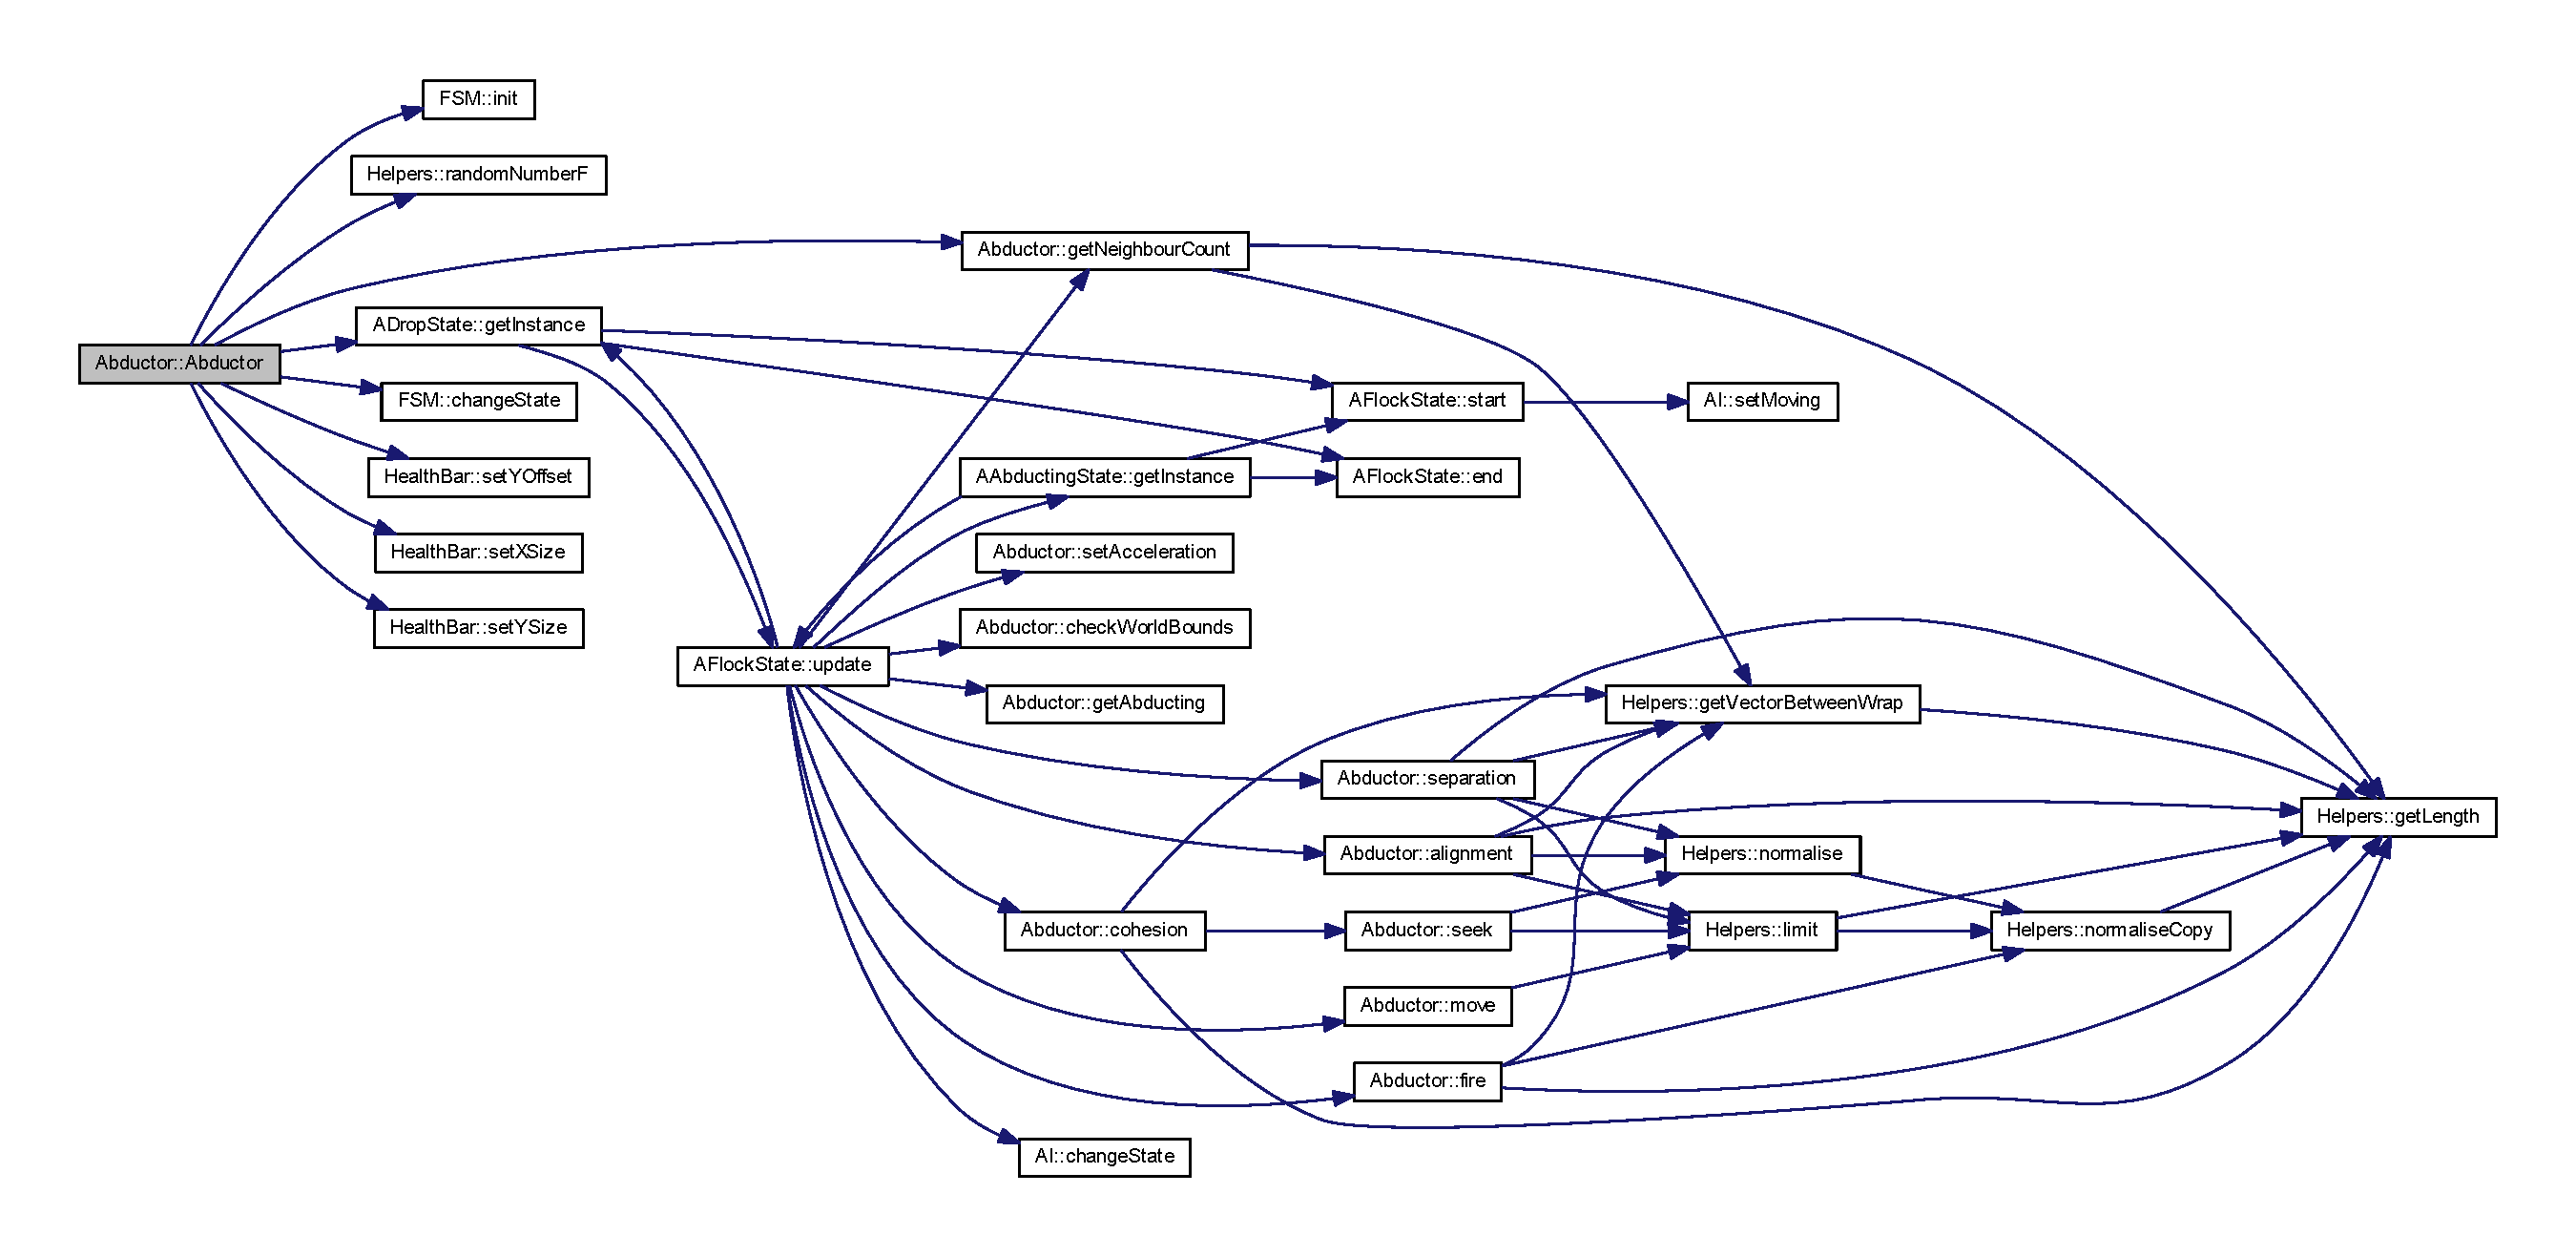
\includegraphics[width=350pt]{class_abductor_ac68525ef8d05680afbef24761e2baa8c_cgraph}
\end{center}
\end{figure}


\subsection{Member Function Documentation}
\mbox{\Hypertarget{class_abductor_ac8ef27110672980a395fa9ba68299337}\label{class_abductor_ac8ef27110672980a395fa9ba68299337}} 
\index{Abductor@{Abductor}!alignment@{alignment}}
\index{alignment@{alignment}!Abductor@{Abductor}}
\subsubsection{\texorpdfstring{alignment()}{alignment()}}
{\footnotesize\ttfamily sf\+::\+Vector2f Abductor\+::alignment (\begin{DoxyParamCaption}{ }\end{DoxyParamCaption})}

Here is the call graph for this function\+:
\nopagebreak
\begin{figure}[H]
\begin{center}
\leavevmode
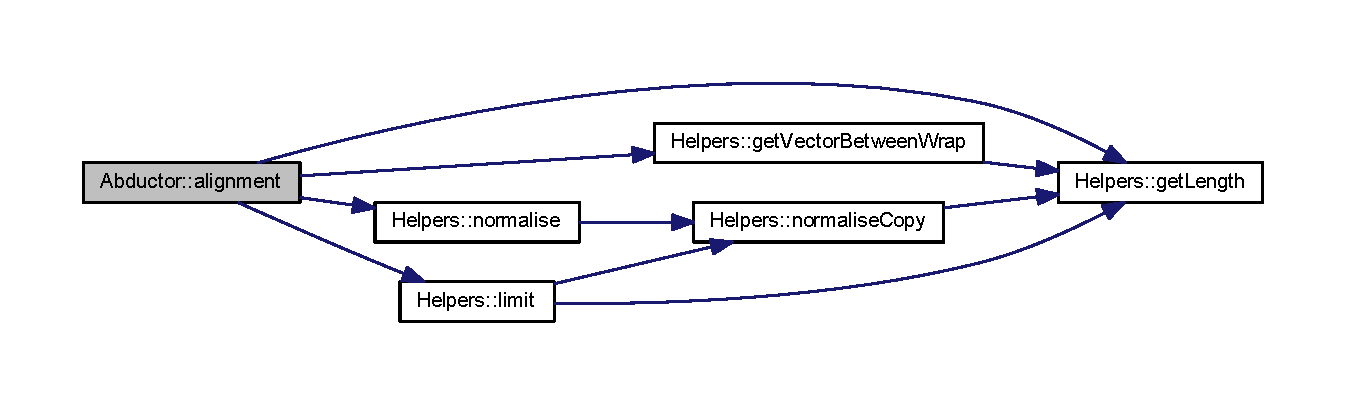
\includegraphics[width=350pt]{class_abductor_ac8ef27110672980a395fa9ba68299337_cgraph}
\end{center}
\end{figure}
Here is the caller graph for this function\+:
\nopagebreak
\begin{figure}[H]
\begin{center}
\leavevmode
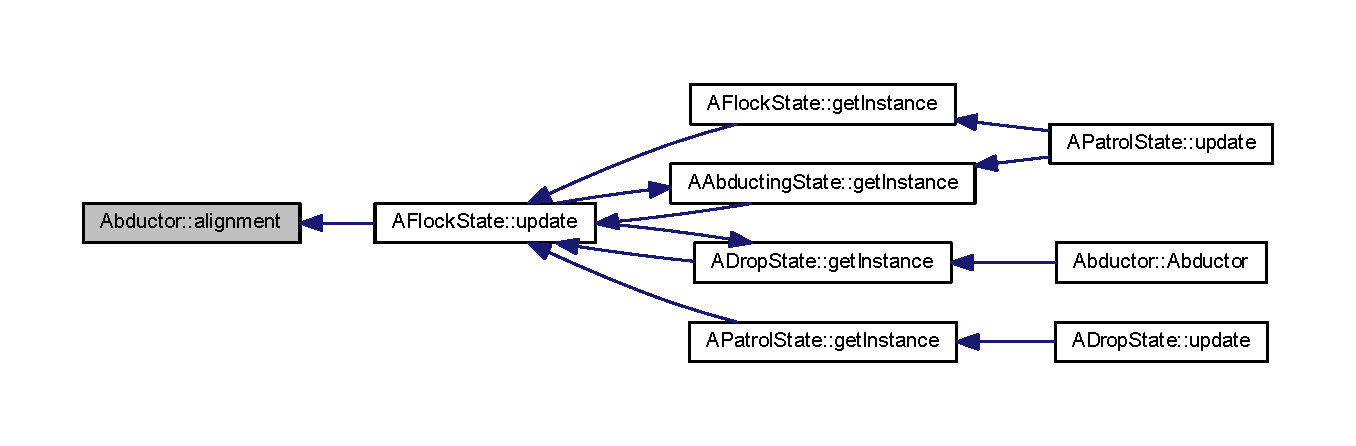
\includegraphics[width=350pt]{class_abductor_ac8ef27110672980a395fa9ba68299337_icgraph}
\end{center}
\end{figure}
\mbox{\Hypertarget{class_abductor_a1a0d06816d3572995a0ce1e0426c6d68}\label{class_abductor_a1a0d06816d3572995a0ce1e0426c6d68}} 
\index{Abductor@{Abductor}!check\+Abduction\+Bounds@{check\+Abduction\+Bounds}}
\index{check\+Abduction\+Bounds@{check\+Abduction\+Bounds}!Abductor@{Abductor}}
\subsubsection{\texorpdfstring{check\+Abduction\+Bounds()}{checkAbductionBounds()}}
{\footnotesize\ttfamily void Abductor\+::check\+Abduction\+Bounds (\begin{DoxyParamCaption}{ }\end{DoxyParamCaption})}

Here is the caller graph for this function\+:
\nopagebreak
\begin{figure}[H]
\begin{center}
\leavevmode
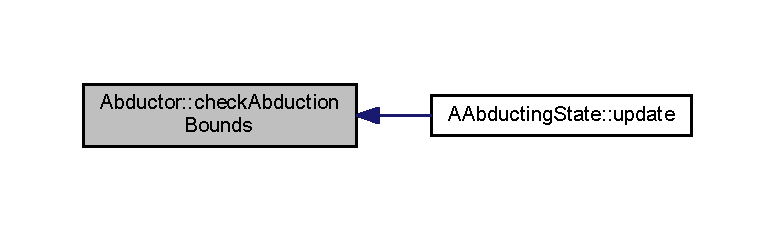
\includegraphics[width=350pt]{class_abductor_a1a0d06816d3572995a0ce1e0426c6d68_icgraph}
\end{center}
\end{figure}
\mbox{\Hypertarget{class_abductor_acbe9315d3199bb9231c0a3d45d07d8f6}\label{class_abductor_acbe9315d3199bb9231c0a3d45d07d8f6}} 
\index{Abductor@{Abductor}!check\+If\+Victim@{check\+If\+Victim}}
\index{check\+If\+Victim@{check\+If\+Victim}!Abductor@{Abductor}}
\subsubsection{\texorpdfstring{check\+If\+Victim()}{checkIfVictim()}}
{\footnotesize\ttfamily bool Abductor\+::check\+If\+Victim (\begin{DoxyParamCaption}\item[{const std\+::shared\+\_\+ptr$<$ \hyperlink{class_game_object}{Game\+Object} $>$ \&}]{astro\+Object }\end{DoxyParamCaption})}

Here is the call graph for this function\+:
\nopagebreak
\begin{figure}[H]
\begin{center}
\leavevmode
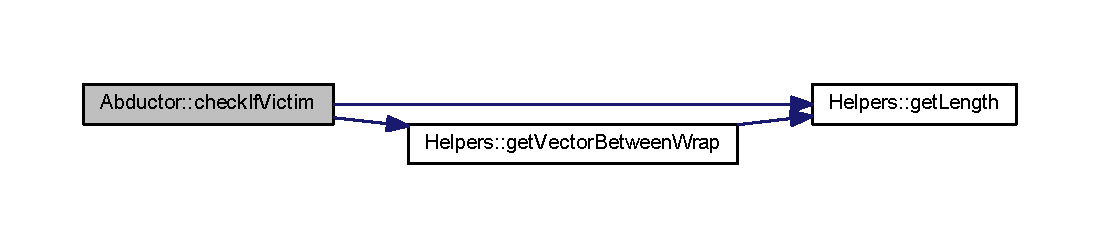
\includegraphics[width=350pt]{class_abductor_acbe9315d3199bb9231c0a3d45d07d8f6_cgraph}
\end{center}
\end{figure}
\mbox{\Hypertarget{class_abductor_a4b86fdcd63a060c53da22f092a113b24}\label{class_abductor_a4b86fdcd63a060c53da22f092a113b24}} 
\index{Abductor@{Abductor}!check\+World\+Bounds@{check\+World\+Bounds}}
\index{check\+World\+Bounds@{check\+World\+Bounds}!Abductor@{Abductor}}
\subsubsection{\texorpdfstring{check\+World\+Bounds()}{checkWorldBounds()}}
{\footnotesize\ttfamily void Abductor\+::check\+World\+Bounds (\begin{DoxyParamCaption}{ }\end{DoxyParamCaption})\hspace{0.3cm}{\ttfamily [override]}, {\ttfamily [virtual]}}



Reimplemented from \hyperlink{class_game_object_a07bcaf0d87bd507f0a6e98abebd70e53}{Game\+Object}.

Here is the caller graph for this function\+:
\nopagebreak
\begin{figure}[H]
\begin{center}
\leavevmode
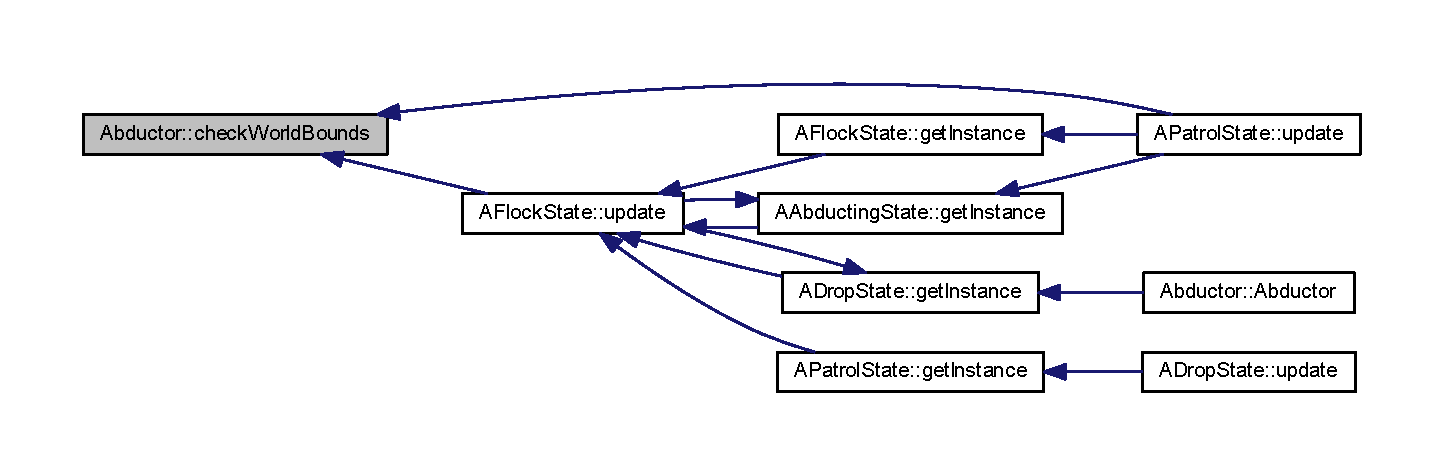
\includegraphics[width=350pt]{class_abductor_a4b86fdcd63a060c53da22f092a113b24_icgraph}
\end{center}
\end{figure}
\mbox{\Hypertarget{class_abductor_ad1660967efd5c4abcdee49989a966722}\label{class_abductor_ad1660967efd5c4abcdee49989a966722}} 
\index{Abductor@{Abductor}!cohesion@{cohesion}}
\index{cohesion@{cohesion}!Abductor@{Abductor}}
\subsubsection{\texorpdfstring{cohesion()}{cohesion()}}
{\footnotesize\ttfamily sf\+::\+Vector2f Abductor\+::cohesion (\begin{DoxyParamCaption}{ }\end{DoxyParamCaption})}

Here is the call graph for this function\+:
\nopagebreak
\begin{figure}[H]
\begin{center}
\leavevmode
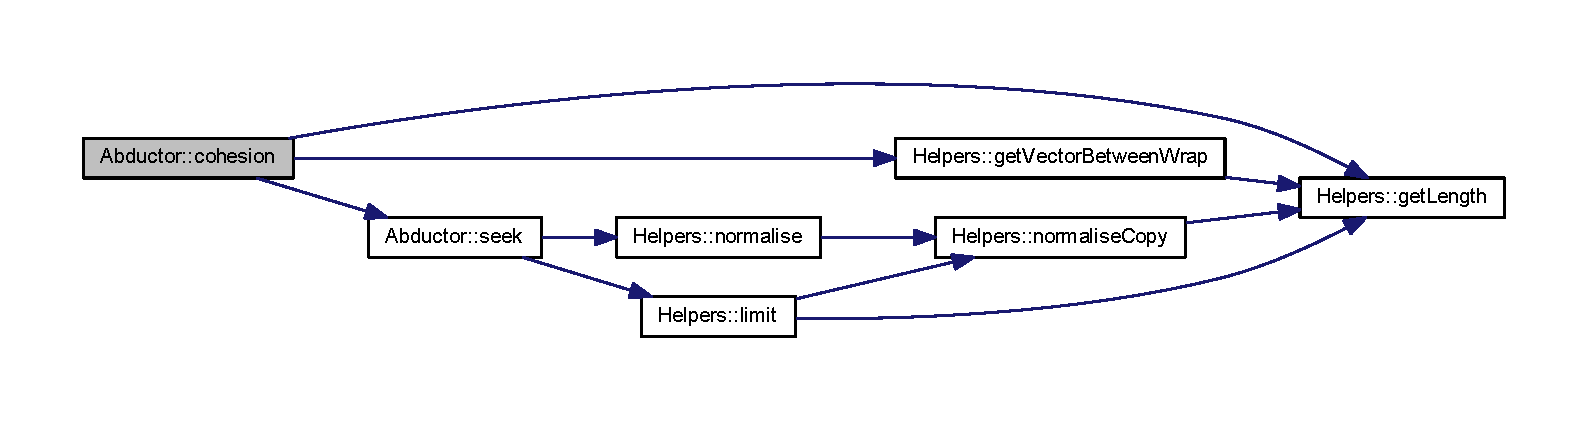
\includegraphics[width=350pt]{class_abductor_ad1660967efd5c4abcdee49989a966722_cgraph}
\end{center}
\end{figure}
Here is the caller graph for this function\+:
\nopagebreak
\begin{figure}[H]
\begin{center}
\leavevmode
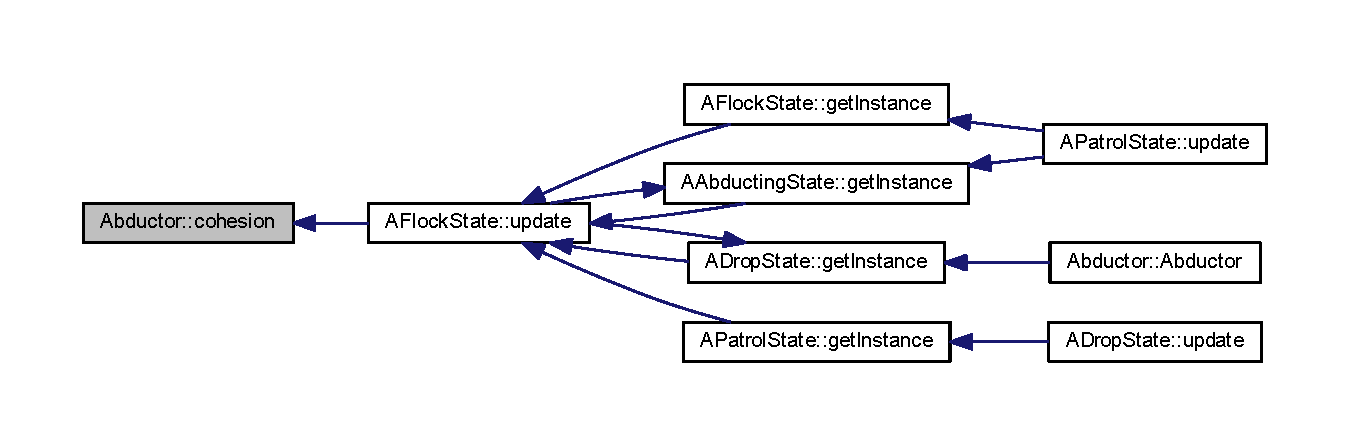
\includegraphics[width=350pt]{class_abductor_ad1660967efd5c4abcdee49989a966722_icgraph}
\end{center}
\end{figure}
\mbox{\Hypertarget{class_abductor_a247dff8e49fc656700c8cb16ed08252d}\label{class_abductor_a247dff8e49fc656700c8cb16ed08252d}} 
\index{Abductor@{Abductor}!collision@{collision}}
\index{collision@{collision}!Abductor@{Abductor}}
\subsubsection{\texorpdfstring{collision()}{collision()}}
{\footnotesize\ttfamily bool Abductor\+::collision (\begin{DoxyParamCaption}\item[{const std\+::shared\+\_\+ptr$<$ \hyperlink{class_game_object}{Game\+Object} $>$ \&}]{collidor }\end{DoxyParamCaption})\hspace{0.3cm}{\ttfamily [override]}, {\ttfamily [virtual]}}



Reimplemented from \hyperlink{class_a_i_a15f7ffd56bf48c7475f9b50d82b60528}{A\+I$<$ Abductor $>$}.

Here is the call graph for this function\+:
\nopagebreak
\begin{figure}[H]
\begin{center}
\leavevmode
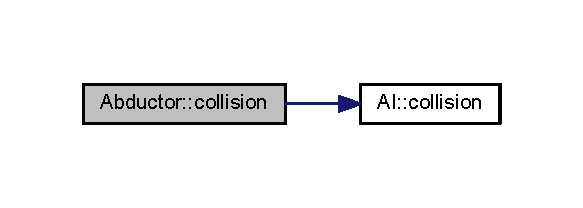
\includegraphics[width=280pt]{class_abductor_a247dff8e49fc656700c8cb16ed08252d_cgraph}
\end{center}
\end{figure}
\mbox{\Hypertarget{class_abductor_aebaf5c5a2882f41c8e1ed1b18f80e3d1}\label{class_abductor_aebaf5c5a2882f41c8e1ed1b18f80e3d1}} 
\index{Abductor@{Abductor}!draw@{draw}}
\index{draw@{draw}!Abductor@{Abductor}}
\subsubsection{\texorpdfstring{draw()}{draw()}}
{\footnotesize\ttfamily void Abductor\+::draw (\begin{DoxyParamCaption}\item[{sf\+::\+Render\+Target \&}]{target,  }\item[{sf\+::\+Render\+States}]{states }\end{DoxyParamCaption}) const\hspace{0.3cm}{\ttfamily [virtual]}}



Reimplemented from \hyperlink{class_a_i_a8a7423a8612cfd777f3b5eeae4764d50}{A\+I$<$ Abductor $>$}.

Here is the call graph for this function\+:
\nopagebreak
\begin{figure}[H]
\begin{center}
\leavevmode
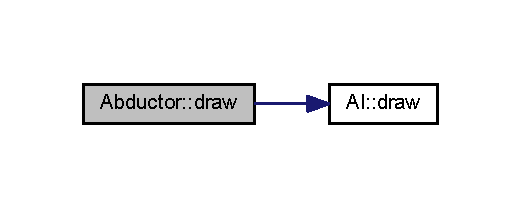
\includegraphics[width=250pt]{class_abductor_aebaf5c5a2882f41c8e1ed1b18f80e3d1_cgraph}
\end{center}
\end{figure}
\mbox{\Hypertarget{class_abductor_a12b84d9d38bec8ed3b495c5657903e50}\label{class_abductor_a12b84d9d38bec8ed3b495c5657903e50}} 
\index{Abductor@{Abductor}!fire@{fire}}
\index{fire@{fire}!Abductor@{Abductor}}
\subsubsection{\texorpdfstring{fire()}{fire()}}
{\footnotesize\ttfamily void Abductor\+::fire (\begin{DoxyParamCaption}\item[{float}]{dt }\end{DoxyParamCaption})}

Here is the call graph for this function\+:
\nopagebreak
\begin{figure}[H]
\begin{center}
\leavevmode
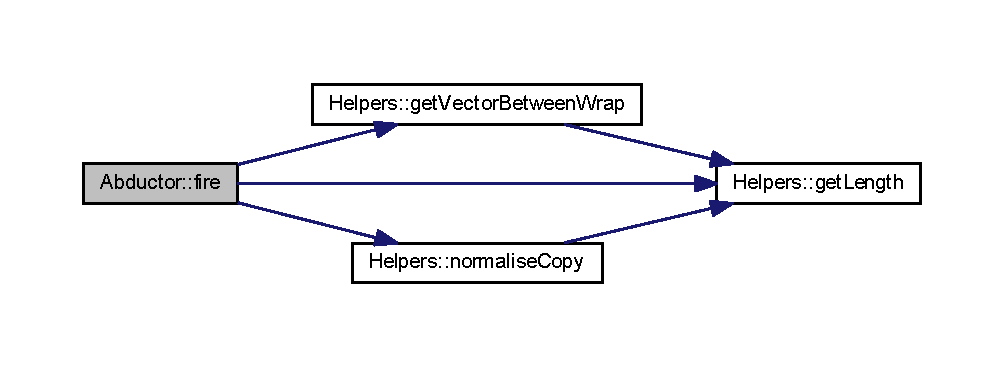
\includegraphics[width=350pt]{class_abductor_a12b84d9d38bec8ed3b495c5657903e50_cgraph}
\end{center}
\end{figure}
Here is the caller graph for this function\+:
\nopagebreak
\begin{figure}[H]
\begin{center}
\leavevmode
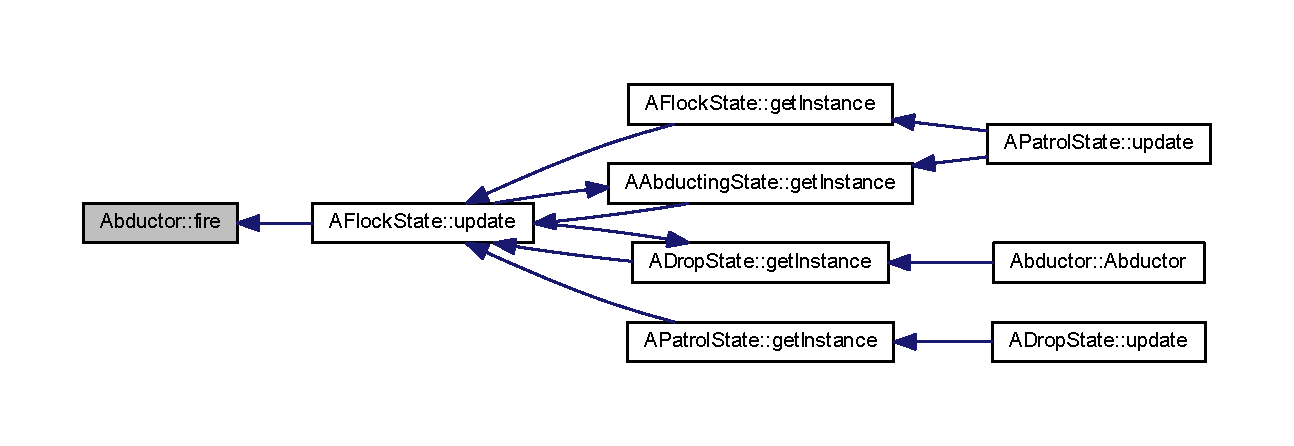
\includegraphics[width=350pt]{class_abductor_a12b84d9d38bec8ed3b495c5657903e50_icgraph}
\end{center}
\end{figure}
\mbox{\Hypertarget{class_abductor_ac0c62963a2e8bdac8c34bfb2a2c0b868}\label{class_abductor_ac0c62963a2e8bdac8c34bfb2a2c0b868}} 
\index{Abductor@{Abductor}!get\+Abducting@{get\+Abducting}}
\index{get\+Abducting@{get\+Abducting}!Abductor@{Abductor}}
\subsubsection{\texorpdfstring{get\+Abducting()}{getAbducting()}}
{\footnotesize\ttfamily bool Abductor\+::get\+Abducting (\begin{DoxyParamCaption}{ }\end{DoxyParamCaption}) const}

Here is the caller graph for this function\+:
\nopagebreak
\begin{figure}[H]
\begin{center}
\leavevmode
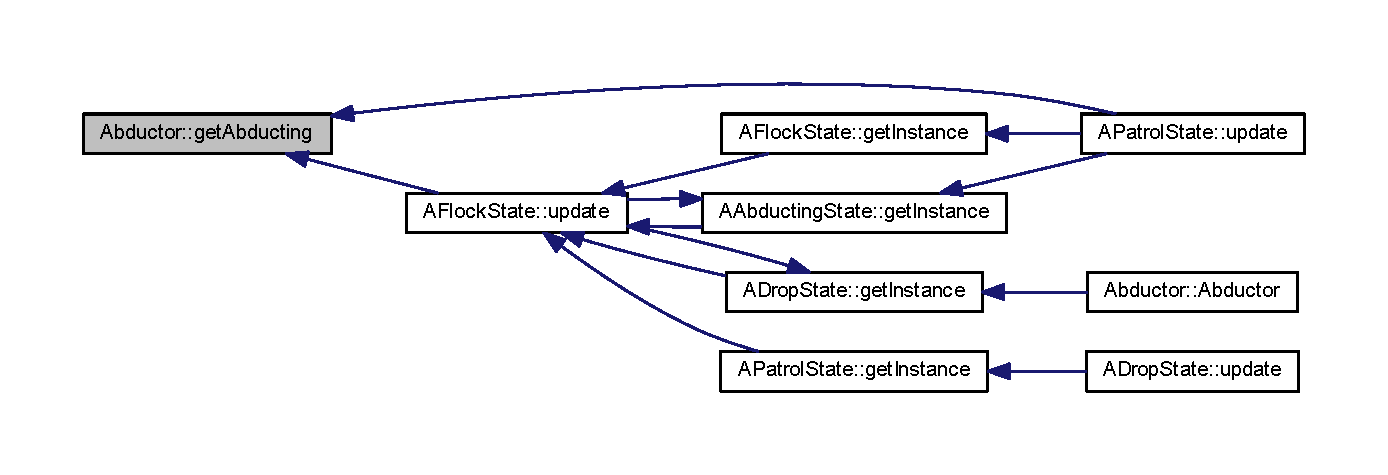
\includegraphics[width=350pt]{class_abductor_ac0c62963a2e8bdac8c34bfb2a2c0b868_icgraph}
\end{center}
\end{figure}
\mbox{\Hypertarget{class_abductor_a30a40083cd604343d7b1d63e1a48a3fa}\label{class_abductor_a30a40083cd604343d7b1d63e1a48a3fa}} 
\index{Abductor@{Abductor}!get\+Direction@{get\+Direction}}
\index{get\+Direction@{get\+Direction}!Abductor@{Abductor}}
\subsubsection{\texorpdfstring{get\+Direction()}{getDirection()}}
{\footnotesize\ttfamily sf\+::\+Vector2f Abductor\+::get\+Direction (\begin{DoxyParamCaption}{ }\end{DoxyParamCaption}) const}

Here is the caller graph for this function\+:
\nopagebreak
\begin{figure}[H]
\begin{center}
\leavevmode
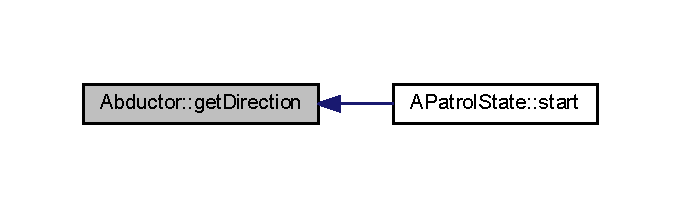
\includegraphics[width=327pt]{class_abductor_a30a40083cd604343d7b1d63e1a48a3fa_icgraph}
\end{center}
\end{figure}
\mbox{\Hypertarget{class_abductor_a8bc04ea46a52e8a58feceee69a8965d0}\label{class_abductor_a8bc04ea46a52e8a58feceee69a8965d0}} 
\index{Abductor@{Abductor}!get\+Force\+Amount@{get\+Force\+Amount}}
\index{get\+Force\+Amount@{get\+Force\+Amount}!Abductor@{Abductor}}
\subsubsection{\texorpdfstring{get\+Force\+Amount()}{getForceAmount()}}
{\footnotesize\ttfamily float Abductor\+::get\+Force\+Amount (\begin{DoxyParamCaption}{ }\end{DoxyParamCaption}) const}

Here is the caller graph for this function\+:
\nopagebreak
\begin{figure}[H]
\begin{center}
\leavevmode
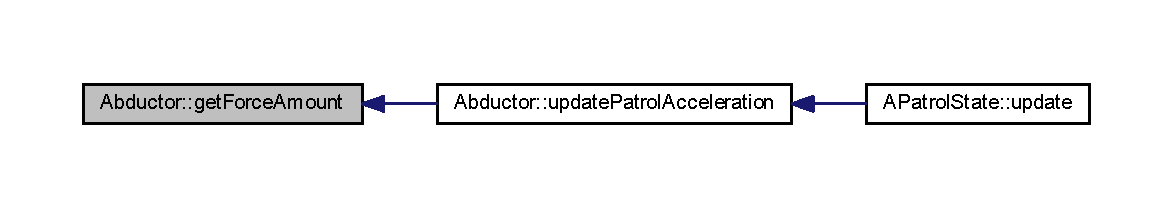
\includegraphics[width=350pt]{class_abductor_a8bc04ea46a52e8a58feceee69a8965d0_icgraph}
\end{center}
\end{figure}
\mbox{\Hypertarget{class_abductor_ae8c4cc87315ccc822d59d73a7c12c94a}\label{class_abductor_ae8c4cc87315ccc822d59d73a7c12c94a}} 
\index{Abductor@{Abductor}!get\+Neighbour\+Count@{get\+Neighbour\+Count}}
\index{get\+Neighbour\+Count@{get\+Neighbour\+Count}!Abductor@{Abductor}}
\subsubsection{\texorpdfstring{get\+Neighbour\+Count()}{getNeighbourCount()}}
{\footnotesize\ttfamily int Abductor\+::get\+Neighbour\+Count (\begin{DoxyParamCaption}{ }\end{DoxyParamCaption}) const}

Here is the call graph for this function\+:
\nopagebreak
\begin{figure}[H]
\begin{center}
\leavevmode
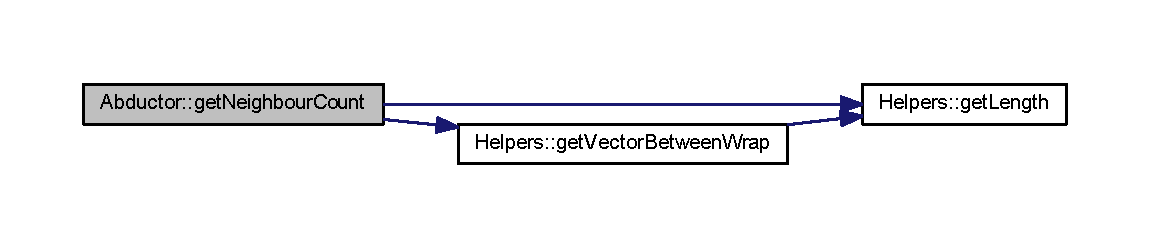
\includegraphics[width=350pt]{class_abductor_ae8c4cc87315ccc822d59d73a7c12c94a_cgraph}
\end{center}
\end{figure}
Here is the caller graph for this function\+:
\nopagebreak
\begin{figure}[H]
\begin{center}
\leavevmode
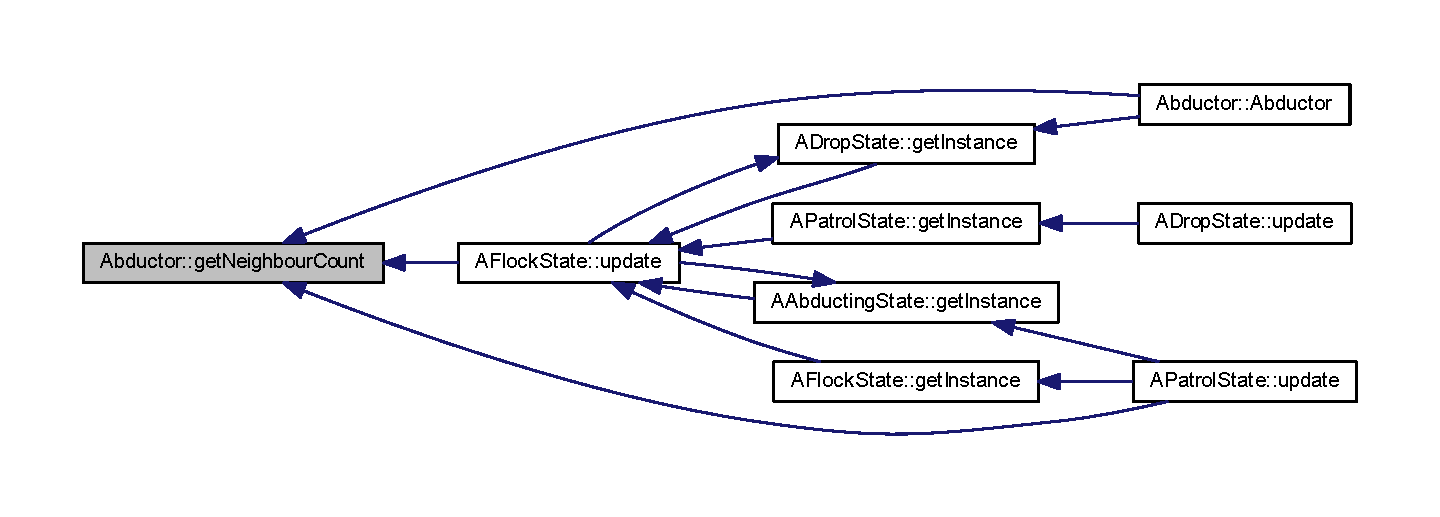
\includegraphics[width=350pt]{class_abductor_ae8c4cc87315ccc822d59d73a7c12c94a_icgraph}
\end{center}
\end{figure}
\mbox{\Hypertarget{class_abductor_a10bb137ba1b1707466f0a893052a0b30}\label{class_abductor_a10bb137ba1b1707466f0a893052a0b30}} 
\index{Abductor@{Abductor}!move@{move}}
\index{move@{move}!Abductor@{Abductor}}
\subsubsection{\texorpdfstring{move()}{move()}}
{\footnotesize\ttfamily void Abductor\+::move (\begin{DoxyParamCaption}\item[{float}]{dt }\end{DoxyParamCaption})\hspace{0.3cm}{\ttfamily [override]}, {\ttfamily [virtual]}}



Reimplemented from \hyperlink{class_game_object_abebe08f70e334c52b8bf052b6ef8c6f3}{Game\+Object}.

Here is the call graph for this function\+:
\nopagebreak
\begin{figure}[H]
\begin{center}
\leavevmode
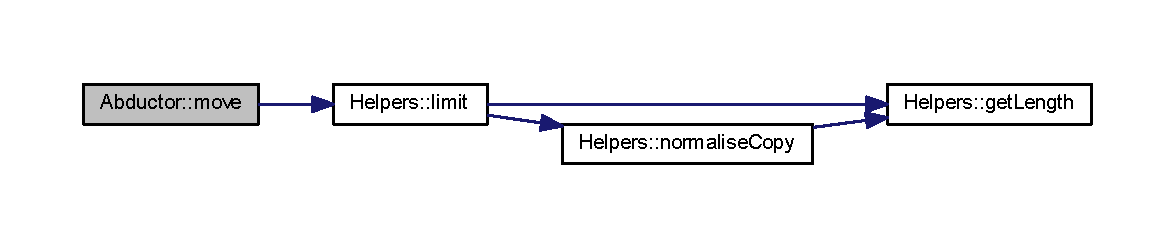
\includegraphics[width=350pt]{class_abductor_a10bb137ba1b1707466f0a893052a0b30_cgraph}
\end{center}
\end{figure}
Here is the caller graph for this function\+:
\nopagebreak
\begin{figure}[H]
\begin{center}
\leavevmode
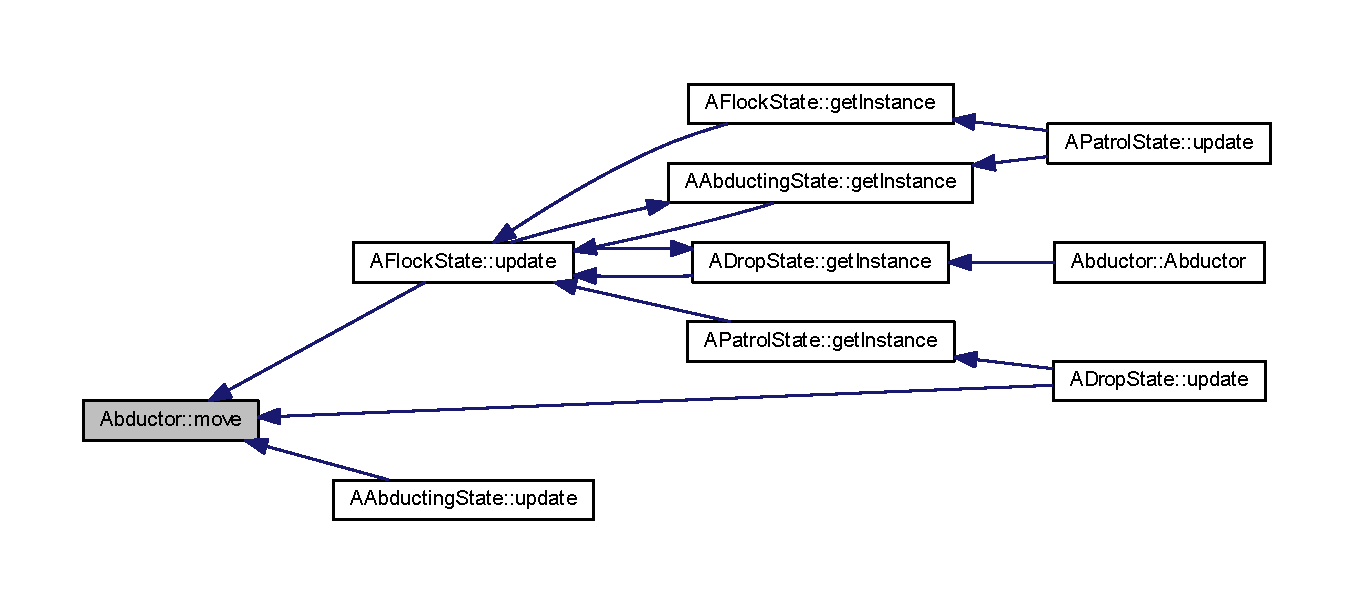
\includegraphics[width=350pt]{class_abductor_a10bb137ba1b1707466f0a893052a0b30_icgraph}
\end{center}
\end{figure}
\mbox{\Hypertarget{class_abductor_acc2841707aaeb5719ecc615b5fe6bf56}\label{class_abductor_acc2841707aaeb5719ecc615b5fe6bf56}} 
\index{Abductor@{Abductor}!reached\+Target@{reached\+Target}}
\index{reached\+Target@{reached\+Target}!Abductor@{Abductor}}
\subsubsection{\texorpdfstring{reached\+Target()}{reachedTarget()}}
{\footnotesize\ttfamily bool Abductor\+::reached\+Target (\begin{DoxyParamCaption}{ }\end{DoxyParamCaption}) const}

Here is the caller graph for this function\+:
\nopagebreak
\begin{figure}[H]
\begin{center}
\leavevmode
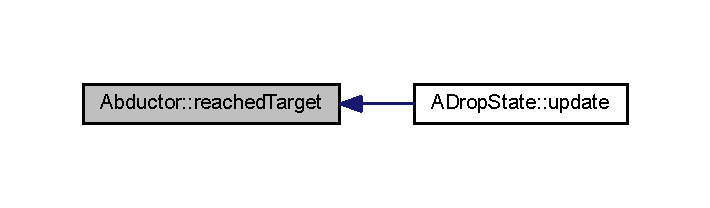
\includegraphics[width=341pt]{class_abductor_acc2841707aaeb5719ecc615b5fe6bf56_icgraph}
\end{center}
\end{figure}
\mbox{\Hypertarget{class_abductor_a2c5431c2d7afa37f9f083762eff5a995}\label{class_abductor_a2c5431c2d7afa37f9f083762eff5a995}} 
\index{Abductor@{Abductor}!seek@{seek}}
\index{seek@{seek}!Abductor@{Abductor}}
\subsubsection{\texorpdfstring{seek()}{seek()}}
{\footnotesize\ttfamily sf\+::\+Vector2f Abductor\+::seek (\begin{DoxyParamCaption}\item[{const sf\+::\+Vector2f \&}]{v }\end{DoxyParamCaption})}

Here is the call graph for this function\+:
\nopagebreak
\begin{figure}[H]
\begin{center}
\leavevmode
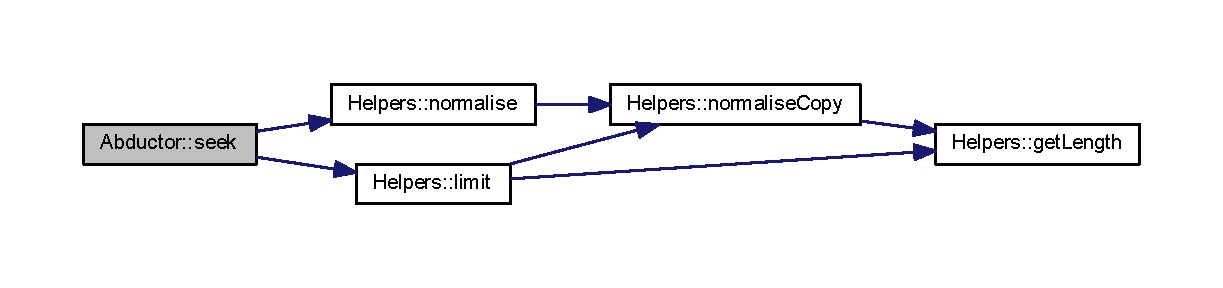
\includegraphics[width=350pt]{class_abductor_a2c5431c2d7afa37f9f083762eff5a995_cgraph}
\end{center}
\end{figure}
Here is the caller graph for this function\+:
\nopagebreak
\begin{figure}[H]
\begin{center}
\leavevmode
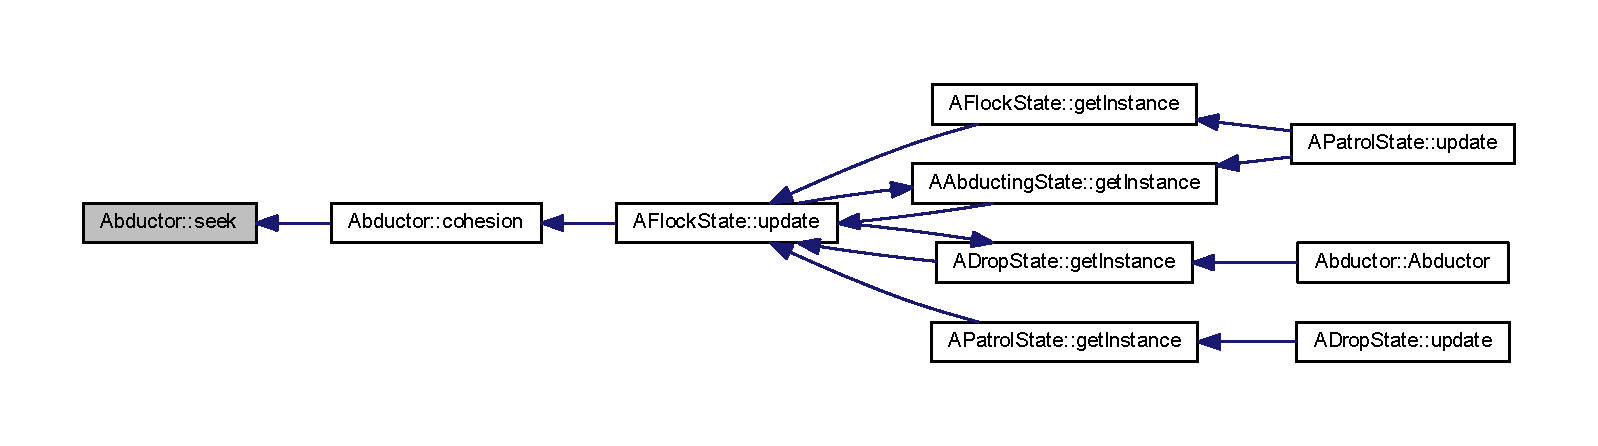
\includegraphics[width=350pt]{class_abductor_a2c5431c2d7afa37f9f083762eff5a995_icgraph}
\end{center}
\end{figure}
\mbox{\Hypertarget{class_abductor_aac2bef46d63d3aa630a34ee1cb23a7f6}\label{class_abductor_aac2bef46d63d3aa630a34ee1cb23a7f6}} 
\index{Abductor@{Abductor}!separation@{separation}}
\index{separation@{separation}!Abductor@{Abductor}}
\subsubsection{\texorpdfstring{separation()}{separation()}}
{\footnotesize\ttfamily sf\+::\+Vector2f Abductor\+::separation (\begin{DoxyParamCaption}{ }\end{DoxyParamCaption})}

Here is the call graph for this function\+:
\nopagebreak
\begin{figure}[H]
\begin{center}
\leavevmode
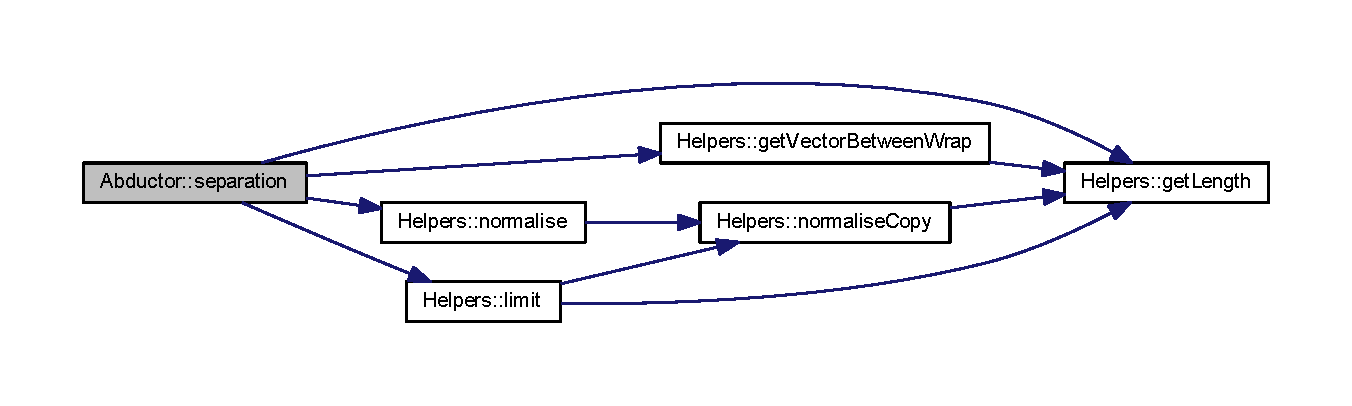
\includegraphics[width=350pt]{class_abductor_aac2bef46d63d3aa630a34ee1cb23a7f6_cgraph}
\end{center}
\end{figure}
Here is the caller graph for this function\+:
\nopagebreak
\begin{figure}[H]
\begin{center}
\leavevmode
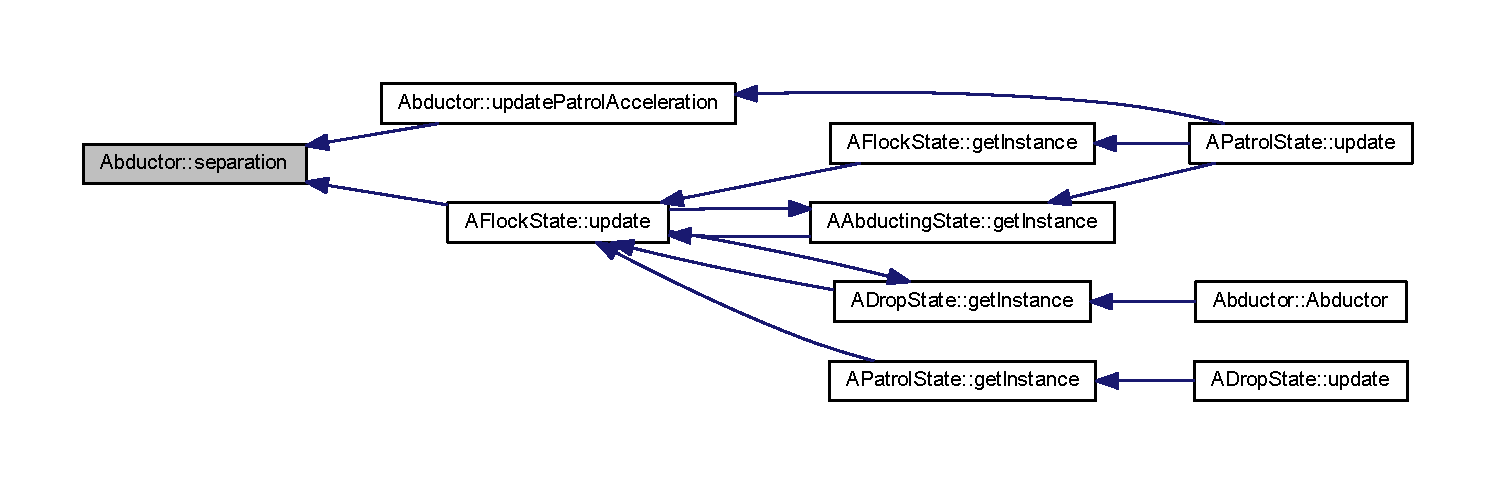
\includegraphics[width=350pt]{class_abductor_aac2bef46d63d3aa630a34ee1cb23a7f6_icgraph}
\end{center}
\end{figure}
\mbox{\Hypertarget{class_abductor_a1069f5de8e0696be938a741f4b931855}\label{class_abductor_a1069f5de8e0696be938a741f4b931855}} 
\index{Abductor@{Abductor}!set\+Abducting@{set\+Abducting}}
\index{set\+Abducting@{set\+Abducting}!Abductor@{Abductor}}
\subsubsection{\texorpdfstring{set\+Abducting()}{setAbducting()}}
{\footnotesize\ttfamily void Abductor\+::set\+Abducting (\begin{DoxyParamCaption}\item[{bool}]{value }\end{DoxyParamCaption})}

\mbox{\Hypertarget{class_abductor_a20e45bb3b4a18f7d5baeb697d1e5b1d5}\label{class_abductor_a20e45bb3b4a18f7d5baeb697d1e5b1d5}} 
\index{Abductor@{Abductor}!set\+Abducting\+Victim@{set\+Abducting\+Victim}}
\index{set\+Abducting\+Victim@{set\+Abducting\+Victim}!Abductor@{Abductor}}
\subsubsection{\texorpdfstring{set\+Abducting\+Victim()}{setAbductingVictim()}}
{\footnotesize\ttfamily void Abductor\+::set\+Abducting\+Victim (\begin{DoxyParamCaption}\item[{const std\+::shared\+\_\+ptr$<$ \hyperlink{class_astronaut}{Astronaut} $>$ \&}]{abduction\+Victim }\end{DoxyParamCaption})}

\mbox{\Hypertarget{class_abductor_a7147793ce13d446f83eb52920dfa15f7}\label{class_abductor_a7147793ce13d446f83eb52920dfa15f7}} 
\index{Abductor@{Abductor}!set\+Acceleration@{set\+Acceleration}}
\index{set\+Acceleration@{set\+Acceleration}!Abductor@{Abductor}}
\subsubsection{\texorpdfstring{set\+Acceleration()}{setAcceleration()}}
{\footnotesize\ttfamily void Abductor\+::set\+Acceleration (\begin{DoxyParamCaption}\item[{const sf\+::\+Vector2f \&}]{acceleration }\end{DoxyParamCaption})}

Here is the caller graph for this function\+:
\nopagebreak
\begin{figure}[H]
\begin{center}
\leavevmode
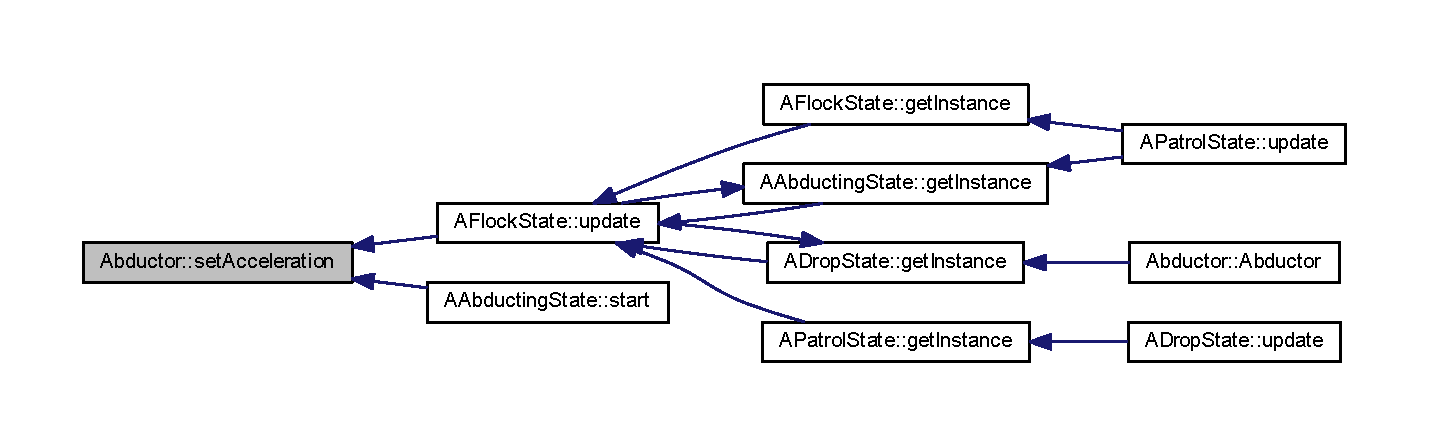
\includegraphics[width=350pt]{class_abductor_a7147793ce13d446f83eb52920dfa15f7_icgraph}
\end{center}
\end{figure}
\mbox{\Hypertarget{class_abductor_aad7a615477ffe510984c8df16e98c903}\label{class_abductor_aad7a615477ffe510984c8df16e98c903}} 
\index{Abductor@{Abductor}!set\+Direction@{set\+Direction}}
\index{set\+Direction@{set\+Direction}!Abductor@{Abductor}}
\subsubsection{\texorpdfstring{set\+Direction()}{setDirection()}}
{\footnotesize\ttfamily void Abductor\+::set\+Direction (\begin{DoxyParamCaption}\item[{const sf\+::\+Vector2f \&}]{dir }\end{DoxyParamCaption})}

Here is the caller graph for this function\+:
\nopagebreak
\begin{figure}[H]
\begin{center}
\leavevmode
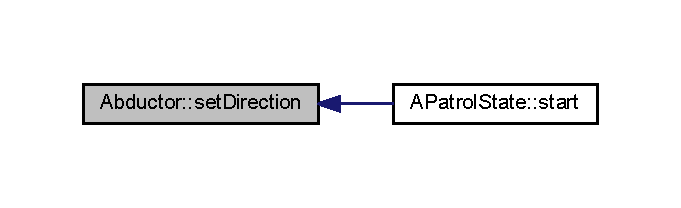
\includegraphics[width=327pt]{class_abductor_aad7a615477ffe510984c8df16e98c903_icgraph}
\end{center}
\end{figure}
\mbox{\Hypertarget{class_abductor_ac30f2067a89f27befe9651cae8b5bca6}\label{class_abductor_ac30f2067a89f27befe9651cae8b5bca6}} 
\index{Abductor@{Abductor}!stop\+Abducting@{stop\+Abducting}}
\index{stop\+Abducting@{stop\+Abducting}!Abductor@{Abductor}}
\subsubsection{\texorpdfstring{stop\+Abducting()}{stopAbducting()}}
{\footnotesize\ttfamily void Abductor\+::stop\+Abducting (\begin{DoxyParamCaption}{ }\end{DoxyParamCaption})}

Here is the caller graph for this function\+:
\nopagebreak
\begin{figure}[H]
\begin{center}
\leavevmode
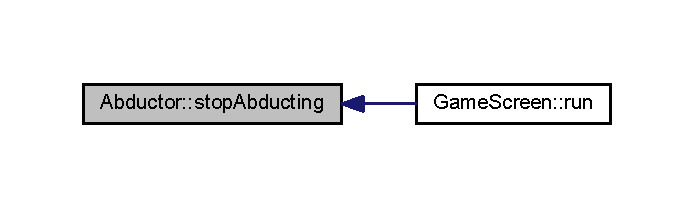
\includegraphics[width=333pt]{class_abductor_ac30f2067a89f27befe9651cae8b5bca6_icgraph}
\end{center}
\end{figure}
\mbox{\Hypertarget{class_abductor_aa9e1628fe605674f599b1ff535c31ac1}\label{class_abductor_aa9e1628fe605674f599b1ff535c31ac1}} 
\index{Abductor@{Abductor}!update\+Abduction@{update\+Abduction}}
\index{update\+Abduction@{update\+Abduction}!Abductor@{Abductor}}
\subsubsection{\texorpdfstring{update\+Abduction()}{updateAbduction()}}
{\footnotesize\ttfamily void Abductor\+::update\+Abduction (\begin{DoxyParamCaption}\item[{float}]{dt }\end{DoxyParamCaption})}

Here is the call graph for this function\+:
\nopagebreak
\begin{figure}[H]
\begin{center}
\leavevmode
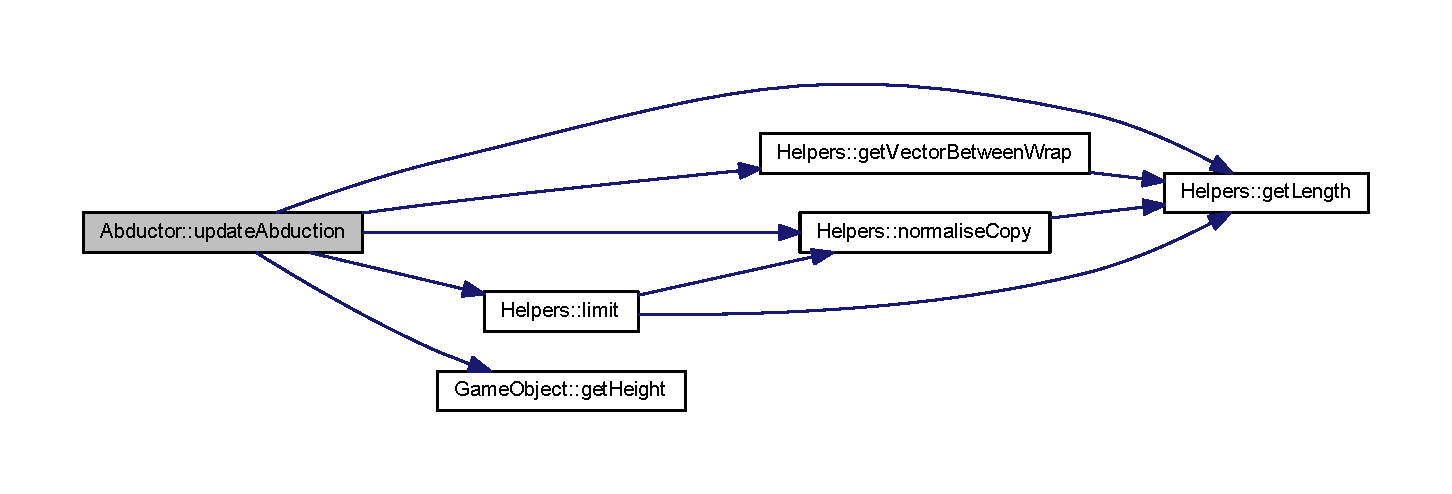
\includegraphics[width=350pt]{class_abductor_aa9e1628fe605674f599b1ff535c31ac1_cgraph}
\end{center}
\end{figure}
Here is the caller graph for this function\+:
\nopagebreak
\begin{figure}[H]
\begin{center}
\leavevmode
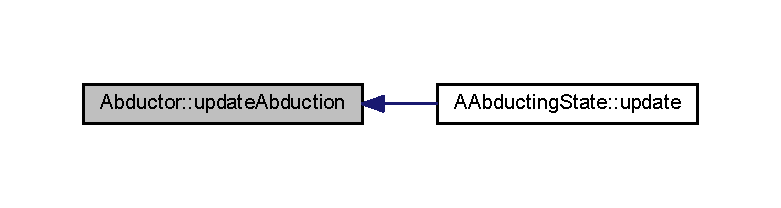
\includegraphics[width=350pt]{class_abductor_aa9e1628fe605674f599b1ff535c31ac1_icgraph}
\end{center}
\end{figure}
\mbox{\Hypertarget{class_abductor_aab823ab3fd94214f90b003661e036d03}\label{class_abductor_aab823ab3fd94214f90b003661e036d03}} 
\index{Abductor@{Abductor}!update\+Drop\+Acceleration@{update\+Drop\+Acceleration}}
\index{update\+Drop\+Acceleration@{update\+Drop\+Acceleration}!Abductor@{Abductor}}
\subsubsection{\texorpdfstring{update\+Drop\+Acceleration()}{updateDropAcceleration()}}
{\footnotesize\ttfamily void Abductor\+::update\+Drop\+Acceleration (\begin{DoxyParamCaption}{ }\end{DoxyParamCaption})}

Here is the call graph for this function\+:
\nopagebreak
\begin{figure}[H]
\begin{center}
\leavevmode
\includegraphics[width=350pt]{class_abductor_aab823ab3fd94214f90b003661e036d03_cgraph}
\end{center}
\end{figure}
Here is the caller graph for this function\+:
\nopagebreak
\begin{figure}[H]
\begin{center}
\leavevmode
\includegraphics[width=350pt]{class_abductor_aab823ab3fd94214f90b003661e036d03_icgraph}
\end{center}
\end{figure}
\mbox{\Hypertarget{class_abductor_a24cc63afd005eef7d1ed694933a2c2a0}\label{class_abductor_a24cc63afd005eef7d1ed694933a2c2a0}} 
\index{Abductor@{Abductor}!update\+Patrol\+Acceleration@{update\+Patrol\+Acceleration}}
\index{update\+Patrol\+Acceleration@{update\+Patrol\+Acceleration}!Abductor@{Abductor}}
\subsubsection{\texorpdfstring{update\+Patrol\+Acceleration()}{updatePatrolAcceleration()}}
{\footnotesize\ttfamily void Abductor\+::update\+Patrol\+Acceleration (\begin{DoxyParamCaption}{ }\end{DoxyParamCaption})}

Here is the call graph for this function\+:
\nopagebreak
\begin{figure}[H]
\begin{center}
\leavevmode
\includegraphics[width=350pt]{class_abductor_a24cc63afd005eef7d1ed694933a2c2a0_cgraph}
\end{center}
\end{figure}
Here is the caller graph for this function\+:
\nopagebreak
\begin{figure}[H]
\begin{center}
\leavevmode
\includegraphics[width=350pt]{class_abductor_a24cc63afd005eef7d1ed694933a2c2a0_icgraph}
\end{center}
\end{figure}


The documentation for this class was generated from the following files\+:\begin{DoxyCompactItemize}
\item 
include/\hyperlink{_abductor_8h}{Abductor.\+h}\item 
src/\hyperlink{_abductor_8cpp}{Abductor.\+cpp}\end{DoxyCompactItemize}

\hypertarget{class_a_drop_state}{}\section{A\+Drop\+State Class Reference}
\label{class_a_drop_state}\index{A\+Drop\+State@{A\+Drop\+State}}


{\ttfamily \#include $<$Abductor\+States.\+h$>$}



Inheritance diagram for A\+Drop\+State\+:
\nopagebreak
\begin{figure}[H]
\begin{center}
\leavevmode
\includegraphics[width=177pt]{class_a_drop_state__inherit__graph}
\end{center}
\end{figure}


Collaboration diagram for A\+Drop\+State\+:
\nopagebreak
\begin{figure}[H]
\begin{center}
\leavevmode
\includegraphics[width=177pt]{class_a_drop_state__coll__graph}
\end{center}
\end{figure}
\subsection*{Public Member Functions}
\begin{DoxyCompactItemize}
\item 
void \hyperlink{class_a_drop_state_ab41abe3006ca9d4dec5e93a800a03e01}{start} (\hyperlink{class_abductor}{Abductor} $\ast$) override
\item 
void \hyperlink{class_a_drop_state_a50ee2cafa31714ee14223e6cce007f08}{update} (\hyperlink{class_abductor}{Abductor} $\ast$, float) override
\item 
void \hyperlink{class_a_drop_state_a6af566dd1e06d425f16a69bbd11e811f}{end} (\hyperlink{class_abductor}{Abductor} $\ast$) override
\end{DoxyCompactItemize}
\subsection*{Static Public Member Functions}
\begin{DoxyCompactItemize}
\item 
static std\+::shared\+\_\+ptr$<$ \hyperlink{class_a_drop_state}{A\+Drop\+State} $>$ \& \hyperlink{class_a_drop_state_a836c382a58447787d3c1518cccea8ebc}{get\+Instance} ()
\end{DoxyCompactItemize}
\subsection*{Additional Inherited Members}


\subsection{Member Function Documentation}
\mbox{\Hypertarget{class_a_drop_state_a6af566dd1e06d425f16a69bbd11e811f}\label{class_a_drop_state_a6af566dd1e06d425f16a69bbd11e811f}} 
\index{A\+Drop\+State@{A\+Drop\+State}!end@{end}}
\index{end@{end}!A\+Drop\+State@{A\+Drop\+State}}
\subsubsection{\texorpdfstring{end()}{end()}}
{\footnotesize\ttfamily void A\+Drop\+State\+::end (\begin{DoxyParamCaption}\item[{\hyperlink{class_abductor}{Abductor} $\ast$}]{abductor }\end{DoxyParamCaption})\hspace{0.3cm}{\ttfamily [override]}, {\ttfamily [virtual]}}



Implements \hyperlink{class_state_a97d058722f988c008e912a0e5ec879b3}{State$<$ Abductor $>$}.

\mbox{\Hypertarget{class_a_drop_state_a836c382a58447787d3c1518cccea8ebc}\label{class_a_drop_state_a836c382a58447787d3c1518cccea8ebc}} 
\index{A\+Drop\+State@{A\+Drop\+State}!get\+Instance@{get\+Instance}}
\index{get\+Instance@{get\+Instance}!A\+Drop\+State@{A\+Drop\+State}}
\subsubsection{\texorpdfstring{get\+Instance()}{getInstance()}}
{\footnotesize\ttfamily static std\+::shared\+\_\+ptr$<$\hyperlink{class_a_drop_state}{A\+Drop\+State}$>$\& A\+Drop\+State\+::get\+Instance (\begin{DoxyParamCaption}{ }\end{DoxyParamCaption})\hspace{0.3cm}{\ttfamily [inline]}, {\ttfamily [static]}}

Here is the call graph for this function\+:
\nopagebreak
\begin{figure}[H]
\begin{center}
\leavevmode
\includegraphics[width=350pt]{class_a_drop_state_a836c382a58447787d3c1518cccea8ebc_cgraph}
\end{center}
\end{figure}
Here is the caller graph for this function\+:
\nopagebreak
\begin{figure}[H]
\begin{center}
\leavevmode
\includegraphics[width=350pt]{class_a_drop_state_a836c382a58447787d3c1518cccea8ebc_icgraph}
\end{center}
\end{figure}
\mbox{\Hypertarget{class_a_drop_state_ab41abe3006ca9d4dec5e93a800a03e01}\label{class_a_drop_state_ab41abe3006ca9d4dec5e93a800a03e01}} 
\index{A\+Drop\+State@{A\+Drop\+State}!start@{start}}
\index{start@{start}!A\+Drop\+State@{A\+Drop\+State}}
\subsubsection{\texorpdfstring{start()}{start()}}
{\footnotesize\ttfamily void A\+Drop\+State\+::start (\begin{DoxyParamCaption}\item[{\hyperlink{class_abductor}{Abductor} $\ast$}]{abductor }\end{DoxyParamCaption})\hspace{0.3cm}{\ttfamily [override]}, {\ttfamily [virtual]}}



Implements \hyperlink{class_state_abc29d36b0462a306ac9b32f36571d783}{State$<$ Abductor $>$}.

Here is the call graph for this function\+:
\nopagebreak
\begin{figure}[H]
\begin{center}
\leavevmode
\includegraphics[width=283pt]{class_a_drop_state_ab41abe3006ca9d4dec5e93a800a03e01_cgraph}
\end{center}
\end{figure}
\mbox{\Hypertarget{class_a_drop_state_a50ee2cafa31714ee14223e6cce007f08}\label{class_a_drop_state_a50ee2cafa31714ee14223e6cce007f08}} 
\index{A\+Drop\+State@{A\+Drop\+State}!update@{update}}
\index{update@{update}!A\+Drop\+State@{A\+Drop\+State}}
\subsubsection{\texorpdfstring{update()}{update()}}
{\footnotesize\ttfamily void A\+Drop\+State\+::update (\begin{DoxyParamCaption}\item[{\hyperlink{class_abductor}{Abductor} $\ast$}]{abductor,  }\item[{float}]{dt }\end{DoxyParamCaption})\hspace{0.3cm}{\ttfamily [override]}, {\ttfamily [virtual]}}



Implements \hyperlink{class_state_a30b5f87ed3e3a05fafeaf898e43518ea}{State$<$ Abductor $>$}.

Here is the call graph for this function\+:
\nopagebreak
\begin{figure}[H]
\begin{center}
\leavevmode
\includegraphics[width=350pt]{class_a_drop_state_a50ee2cafa31714ee14223e6cce007f08_cgraph}
\end{center}
\end{figure}


The documentation for this class was generated from the following files\+:\begin{DoxyCompactItemize}
\item 
include/\hyperlink{_abductor_states_8h}{Abductor\+States.\+h}\item 
src/\hyperlink{_abductor_states_8cpp}{Abductor\+States.\+cpp}\end{DoxyCompactItemize}

\hypertarget{class_a_flock_state}{}\section{A\+Flock\+State Class Reference}
\label{class_a_flock_state}\index{A\+Flock\+State@{A\+Flock\+State}}


{\ttfamily \#include $<$Abductor\+States.\+h$>$}



Inheritance diagram for A\+Flock\+State\+:
\nopagebreak
\begin{figure}[H]
\begin{center}
\leavevmode
\includegraphics[width=177pt]{class_a_flock_state__inherit__graph}
\end{center}
\end{figure}


Collaboration diagram for A\+Flock\+State\+:
\nopagebreak
\begin{figure}[H]
\begin{center}
\leavevmode
\includegraphics[width=177pt]{class_a_flock_state__coll__graph}
\end{center}
\end{figure}
\subsection*{Public Member Functions}
\begin{DoxyCompactItemize}
\item 
void \hyperlink{class_a_flock_state_a375255af2422bad8037325ea8ff86ddb}{start} (\hyperlink{class_abductor}{Abductor} $\ast$) override
\item 
void \hyperlink{class_a_flock_state_ac452fa27fac302918460575e5badae91}{update} (\hyperlink{class_abductor}{Abductor} $\ast$, float) override
\item 
void \hyperlink{class_a_flock_state_af81fa7c9e9eb5185e8cd950aceb758f3}{end} (\hyperlink{class_abductor}{Abductor} $\ast$) override
\end{DoxyCompactItemize}
\subsection*{Static Public Member Functions}
\begin{DoxyCompactItemize}
\item 
static std\+::shared\+\_\+ptr$<$ \hyperlink{class_a_flock_state}{A\+Flock\+State} $>$ \& \hyperlink{class_a_flock_state_a838c2fa41a3ff8c863f4bcfe80637c4d}{get\+Instance} ()
\end{DoxyCompactItemize}
\subsection*{Additional Inherited Members}


\subsection{Member Function Documentation}
\mbox{\Hypertarget{class_a_flock_state_af81fa7c9e9eb5185e8cd950aceb758f3}\label{class_a_flock_state_af81fa7c9e9eb5185e8cd950aceb758f3}} 
\index{A\+Flock\+State@{A\+Flock\+State}!end@{end}}
\index{end@{end}!A\+Flock\+State@{A\+Flock\+State}}
\subsubsection{\texorpdfstring{end()}{end()}}
{\footnotesize\ttfamily void A\+Flock\+State\+::end (\begin{DoxyParamCaption}\item[{\hyperlink{class_abductor}{Abductor} $\ast$}]{abductor }\end{DoxyParamCaption})\hspace{0.3cm}{\ttfamily [override]}, {\ttfamily [virtual]}}



Implements \hyperlink{class_state_a97d058722f988c008e912a0e5ec879b3}{State$<$ Abductor $>$}.

Here is the caller graph for this function\+:
\nopagebreak
\begin{figure}[H]
\begin{center}
\leavevmode
\includegraphics[width=350pt]{class_a_flock_state_af81fa7c9e9eb5185e8cd950aceb758f3_icgraph}
\end{center}
\end{figure}
\mbox{\Hypertarget{class_a_flock_state_a838c2fa41a3ff8c863f4bcfe80637c4d}\label{class_a_flock_state_a838c2fa41a3ff8c863f4bcfe80637c4d}} 
\index{A\+Flock\+State@{A\+Flock\+State}!get\+Instance@{get\+Instance}}
\index{get\+Instance@{get\+Instance}!A\+Flock\+State@{A\+Flock\+State}}
\subsubsection{\texorpdfstring{get\+Instance()}{getInstance()}}
{\footnotesize\ttfamily static std\+::shared\+\_\+ptr$<$\hyperlink{class_a_flock_state}{A\+Flock\+State}$>$\& A\+Flock\+State\+::get\+Instance (\begin{DoxyParamCaption}{ }\end{DoxyParamCaption})\hspace{0.3cm}{\ttfamily [inline]}, {\ttfamily [static]}}

Here is the call graph for this function\+:
\nopagebreak
\begin{figure}[H]
\begin{center}
\leavevmode
\includegraphics[width=350pt]{class_a_flock_state_a838c2fa41a3ff8c863f4bcfe80637c4d_cgraph}
\end{center}
\end{figure}
Here is the caller graph for this function\+:
\nopagebreak
\begin{figure}[H]
\begin{center}
\leavevmode
\includegraphics[width=350pt]{class_a_flock_state_a838c2fa41a3ff8c863f4bcfe80637c4d_icgraph}
\end{center}
\end{figure}
\mbox{\Hypertarget{class_a_flock_state_a375255af2422bad8037325ea8ff86ddb}\label{class_a_flock_state_a375255af2422bad8037325ea8ff86ddb}} 
\index{A\+Flock\+State@{A\+Flock\+State}!start@{start}}
\index{start@{start}!A\+Flock\+State@{A\+Flock\+State}}
\subsubsection{\texorpdfstring{start()}{start()}}
{\footnotesize\ttfamily void A\+Flock\+State\+::start (\begin{DoxyParamCaption}\item[{\hyperlink{class_abductor}{Abductor} $\ast$}]{abductor }\end{DoxyParamCaption})\hspace{0.3cm}{\ttfamily [override]}, {\ttfamily [virtual]}}



Implements \hyperlink{class_state_abc29d36b0462a306ac9b32f36571d783}{State$<$ Abductor $>$}.

Here is the call graph for this function\+:
\nopagebreak
\begin{figure}[H]
\begin{center}
\leavevmode
\includegraphics[width=287pt]{class_a_flock_state_a375255af2422bad8037325ea8ff86ddb_cgraph}
\end{center}
\end{figure}
Here is the caller graph for this function\+:
\nopagebreak
\begin{figure}[H]
\begin{center}
\leavevmode
\includegraphics[width=350pt]{class_a_flock_state_a375255af2422bad8037325ea8ff86ddb_icgraph}
\end{center}
\end{figure}
\mbox{\Hypertarget{class_a_flock_state_ac452fa27fac302918460575e5badae91}\label{class_a_flock_state_ac452fa27fac302918460575e5badae91}} 
\index{A\+Flock\+State@{A\+Flock\+State}!update@{update}}
\index{update@{update}!A\+Flock\+State@{A\+Flock\+State}}
\subsubsection{\texorpdfstring{update()}{update()}}
{\footnotesize\ttfamily void A\+Flock\+State\+::update (\begin{DoxyParamCaption}\item[{\hyperlink{class_abductor}{Abductor} $\ast$}]{abductor,  }\item[{float}]{dt }\end{DoxyParamCaption})\hspace{0.3cm}{\ttfamily [override]}, {\ttfamily [virtual]}}



Implements \hyperlink{class_state_a30b5f87ed3e3a05fafeaf898e43518ea}{State$<$ Abductor $>$}.

Here is the call graph for this function\+:
\nopagebreak
\begin{figure}[H]
\begin{center}
\leavevmode
\includegraphics[width=350pt]{class_a_flock_state_ac452fa27fac302918460575e5badae91_cgraph}
\end{center}
\end{figure}
Here is the caller graph for this function\+:
\nopagebreak
\begin{figure}[H]
\begin{center}
\leavevmode
\includegraphics[width=350pt]{class_a_flock_state_ac452fa27fac302918460575e5badae91_icgraph}
\end{center}
\end{figure}


The documentation for this class was generated from the following files\+:\begin{DoxyCompactItemize}
\item 
include/\hyperlink{_abductor_states_8h}{Abductor\+States.\+h}\item 
src/\hyperlink{_abductor_states_8cpp}{Abductor\+States.\+cpp}\end{DoxyCompactItemize}

\hypertarget{class_a_i}{}\section{AI$<$ T $>$ Class Template Reference}
\label{class_a_i}\index{A\+I$<$ T $>$@{A\+I$<$ T $>$}}


{\ttfamily \#include $<$A\+I.\+h$>$}



Inheritance diagram for AI$<$ T $>$\+:\nopagebreak
\begin{figure}[H]
\begin{center}
\leavevmode
\includegraphics[width=151pt]{class_a_i__inherit__graph}
\end{center}
\end{figure}


Collaboration diagram for AI$<$ T $>$\+:\nopagebreak
\begin{figure}[H]
\begin{center}
\leavevmode
\includegraphics[width=232pt]{class_a_i__coll__graph}
\end{center}
\end{figure}
\subsection*{Public Member Functions}
\begin{DoxyCompactItemize}
\item 
\hyperlink{class_a_i_a0e9856d1f5aa1f0009f9ff2cd51e0598}{AI} (\hyperlink{class_game_object_a4bf9e8f660e6a49f1b802c2aa9dd95af}{Game\+Object\+::\+Type} type, const sf\+::\+Vector2f \&start\+Pos, const sf\+::\+Vector2f \&world\+Size)
\item 
void \hyperlink{class_a_i_a1e1875bffd6f4da9e8333cba89aa3cd7}{update} (float dt) override
\item 
void \hyperlink{class_a_i_ae08cb2117d4352ad462fefa357028a82}{change\+State} (std\+::shared\+\_\+ptr$<$ \hyperlink{class_state}{State}$<$ T $>$$>$ state)
\item 
void \hyperlink{class_a_i_ac705298af197a4e87594ee095bfceb60}{set\+Moving} (bool moving)
\item 
virtual bool \hyperlink{class_a_i_a15f7ffd56bf48c7475f9b50d82b60528}{collision} (const std\+::shared\+\_\+ptr$<$ \hyperlink{class_game_object}{Game\+Object} $>$ \&collidor) override
\item 
virtual void \hyperlink{class_a_i_a8a7423a8612cfd777f3b5eeae4764d50}{draw} (sf\+::\+Render\+Target \&target, sf\+::\+Render\+States states) const override
\end{DoxyCompactItemize}
\subsection*{Protected Attributes}
\begin{DoxyCompactItemize}
\item 
const float \hyperlink{class_a_i_a876a6f7273d86861bfbec7ada91c40b0}{L\+O\+W\+E\+S\+T\+\_\+\+D\+I\+S\+T\+A\+N\+CE}
\item 
\hyperlink{class_health_bar}{Health\+Bar} \hyperlink{class_a_i_aa85c378f07b503e706be6cc150a2bae8}{m\+\_\+health\+Bar}
\item 
\hyperlink{class_f_s_m}{F\+SM}$<$ T $>$ \hyperlink{class_a_i_a3411b59aac349775e44e764125a007dd}{m\+\_\+fsm}
\item 
float \hyperlink{class_a_i_ad32aa749623a2cce0d11ea44eb925602}{H\+E\+A\+L\+T\+H\+\_\+\+Y\+\_\+\+O\+F\+F\+S\+ET} = 1.f
\end{DoxyCompactItemize}
\subsection*{Additional Inherited Members}


\subsection{Constructor \& Destructor Documentation}
\mbox{\Hypertarget{class_a_i_a0e9856d1f5aa1f0009f9ff2cd51e0598}\label{class_a_i_a0e9856d1f5aa1f0009f9ff2cd51e0598}} 
\index{AI@{AI}!AI@{AI}}
\index{AI@{AI}!AI@{AI}}
\subsubsection{\texorpdfstring{A\+I()}{AI()}}
{\footnotesize\ttfamily template$<$typename T$>$ \\
\hyperlink{class_a_i}{AI}$<$ T $>$\+::\hyperlink{class_a_i}{AI} (\begin{DoxyParamCaption}\item[{\hyperlink{class_game_object_a4bf9e8f660e6a49f1b802c2aa9dd95af}{Game\+Object\+::\+Type}}]{type,  }\item[{const sf\+::\+Vector2f \&}]{start\+Pos,  }\item[{const sf\+::\+Vector2f \&}]{world\+Size }\end{DoxyParamCaption})\hspace{0.3cm}{\ttfamily [inline]}}



\subsection{Member Function Documentation}
\mbox{\Hypertarget{class_a_i_ae08cb2117d4352ad462fefa357028a82}\label{class_a_i_ae08cb2117d4352ad462fefa357028a82}} 
\index{AI@{AI}!change\+State@{change\+State}}
\index{change\+State@{change\+State}!AI@{AI}}
\subsubsection{\texorpdfstring{change\+State()}{changeState()}}
{\footnotesize\ttfamily template$<$typename T$>$ \\
void \hyperlink{class_a_i}{AI}$<$ T $>$\+::change\+State (\begin{DoxyParamCaption}\item[{std\+::shared\+\_\+ptr$<$ \hyperlink{class_state}{State}$<$ T $>$$>$}]{state }\end{DoxyParamCaption})\hspace{0.3cm}{\ttfamily [inline]}}

Here is the caller graph for this function\+:
\nopagebreak
\begin{figure}[H]
\begin{center}
\leavevmode
\includegraphics[width=350pt]{class_a_i_ae08cb2117d4352ad462fefa357028a82_icgraph}
\end{center}
\end{figure}
\mbox{\Hypertarget{class_a_i_a15f7ffd56bf48c7475f9b50d82b60528}\label{class_a_i_a15f7ffd56bf48c7475f9b50d82b60528}} 
\index{AI@{AI}!collision@{collision}}
\index{collision@{collision}!AI@{AI}}
\subsubsection{\texorpdfstring{collision()}{collision()}}
{\footnotesize\ttfamily template$<$typename T$>$ \\
virtual bool \hyperlink{class_a_i}{AI}$<$ T $>$\+::collision (\begin{DoxyParamCaption}\item[{const std\+::shared\+\_\+ptr$<$ \hyperlink{class_game_object}{Game\+Object} $>$ \&}]{collidor }\end{DoxyParamCaption})\hspace{0.3cm}{\ttfamily [inline]}, {\ttfamily [override]}, {\ttfamily [virtual]}}



Reimplemented from \hyperlink{class_game_object_a56a330813f51b91b2ad8aacb42b6d8ea}{Game\+Object}.



Reimplemented in \hyperlink{class_abductor_a247dff8e49fc656700c8cb16ed08252d}{Abductor}.

Here is the caller graph for this function\+:
\nopagebreak
\begin{figure}[H]
\begin{center}
\leavevmode
\includegraphics[width=280pt]{class_a_i_a15f7ffd56bf48c7475f9b50d82b60528_icgraph}
\end{center}
\end{figure}
\mbox{\Hypertarget{class_a_i_a8a7423a8612cfd777f3b5eeae4764d50}\label{class_a_i_a8a7423a8612cfd777f3b5eeae4764d50}} 
\index{AI@{AI}!draw@{draw}}
\index{draw@{draw}!AI@{AI}}
\subsubsection{\texorpdfstring{draw()}{draw()}}
{\footnotesize\ttfamily template$<$typename T$>$ \\
virtual void \hyperlink{class_a_i}{AI}$<$ T $>$\+::draw (\begin{DoxyParamCaption}\item[{sf\+::\+Render\+Target \&}]{target,  }\item[{sf\+::\+Render\+States}]{states }\end{DoxyParamCaption}) const\hspace{0.3cm}{\ttfamily [inline]}, {\ttfamily [override]}, {\ttfamily [virtual]}}



Reimplemented from \hyperlink{class_game_object_aa6d7650a920e2dd79b0125560faf3807}{Game\+Object}.



Reimplemented in \hyperlink{class_abductor_aebaf5c5a2882f41c8e1ed1b18f80e3d1}{Abductor}.

Here is the caller graph for this function\+:
\nopagebreak
\begin{figure}[H]
\begin{center}
\leavevmode
\includegraphics[width=250pt]{class_a_i_a8a7423a8612cfd777f3b5eeae4764d50_icgraph}
\end{center}
\end{figure}
\mbox{\Hypertarget{class_a_i_ac705298af197a4e87594ee095bfceb60}\label{class_a_i_ac705298af197a4e87594ee095bfceb60}} 
\index{AI@{AI}!set\+Moving@{set\+Moving}}
\index{set\+Moving@{set\+Moving}!AI@{AI}}
\subsubsection{\texorpdfstring{set\+Moving()}{setMoving()}}
{\footnotesize\ttfamily template$<$typename T$>$ \\
void \hyperlink{class_a_i}{AI}$<$ T $>$\+::set\+Moving (\begin{DoxyParamCaption}\item[{bool}]{moving }\end{DoxyParamCaption})\hspace{0.3cm}{\ttfamily [inline]}}

Here is the caller graph for this function\+:
\nopagebreak
\begin{figure}[H]
\begin{center}
\leavevmode
\includegraphics[width=350pt]{class_a_i_ac705298af197a4e87594ee095bfceb60_icgraph}
\end{center}
\end{figure}
\mbox{\Hypertarget{class_a_i_a1e1875bffd6f4da9e8333cba89aa3cd7}\label{class_a_i_a1e1875bffd6f4da9e8333cba89aa3cd7}} 
\index{AI@{AI}!update@{update}}
\index{update@{update}!AI@{AI}}
\subsubsection{\texorpdfstring{update()}{update()}}
{\footnotesize\ttfamily template$<$typename T$>$ \\
void \hyperlink{class_a_i}{AI}$<$ T $>$\+::update (\begin{DoxyParamCaption}\item[{float}]{dt }\end{DoxyParamCaption})\hspace{0.3cm}{\ttfamily [inline]}, {\ttfamily [override]}, {\ttfamily [virtual]}}



Reimplemented from \hyperlink{class_game_object_a2fece397b6343682d639f8943f124d0e}{Game\+Object}.



\subsection{Member Data Documentation}
\mbox{\Hypertarget{class_a_i_ad32aa749623a2cce0d11ea44eb925602}\label{class_a_i_ad32aa749623a2cce0d11ea44eb925602}} 
\index{AI@{AI}!H\+E\+A\+L\+T\+H\+\_\+\+Y\+\_\+\+O\+F\+F\+S\+ET@{H\+E\+A\+L\+T\+H\+\_\+\+Y\+\_\+\+O\+F\+F\+S\+ET}}
\index{H\+E\+A\+L\+T\+H\+\_\+\+Y\+\_\+\+O\+F\+F\+S\+ET@{H\+E\+A\+L\+T\+H\+\_\+\+Y\+\_\+\+O\+F\+F\+S\+ET}!AI@{AI}}
\subsubsection{\texorpdfstring{H\+E\+A\+L\+T\+H\+\_\+\+Y\+\_\+\+O\+F\+F\+S\+ET}{HEALTH\_Y\_OFFSET}}
{\footnotesize\ttfamily template$<$typename T$>$ \\
float \hyperlink{class_a_i}{AI}$<$ T $>$\+::H\+E\+A\+L\+T\+H\+\_\+\+Y\+\_\+\+O\+F\+F\+S\+ET = 1.f\hspace{0.3cm}{\ttfamily [protected]}}

\mbox{\Hypertarget{class_a_i_a876a6f7273d86861bfbec7ada91c40b0}\label{class_a_i_a876a6f7273d86861bfbec7ada91c40b0}} 
\index{AI@{AI}!L\+O\+W\+E\+S\+T\+\_\+\+D\+I\+S\+T\+A\+N\+CE@{L\+O\+W\+E\+S\+T\+\_\+\+D\+I\+S\+T\+A\+N\+CE}}
\index{L\+O\+W\+E\+S\+T\+\_\+\+D\+I\+S\+T\+A\+N\+CE@{L\+O\+W\+E\+S\+T\+\_\+\+D\+I\+S\+T\+A\+N\+CE}!AI@{AI}}
\subsubsection{\texorpdfstring{L\+O\+W\+E\+S\+T\+\_\+\+D\+I\+S\+T\+A\+N\+CE}{LOWEST\_DISTANCE}}
{\footnotesize\ttfamily template$<$typename T$>$ \\
const float \hyperlink{class_a_i}{AI}$<$ T $>$\+::L\+O\+W\+E\+S\+T\+\_\+\+D\+I\+S\+T\+A\+N\+CE\hspace{0.3cm}{\ttfamily [protected]}}

\mbox{\Hypertarget{class_a_i_a3411b59aac349775e44e764125a007dd}\label{class_a_i_a3411b59aac349775e44e764125a007dd}} 
\index{AI@{AI}!m\+\_\+fsm@{m\+\_\+fsm}}
\index{m\+\_\+fsm@{m\+\_\+fsm}!AI@{AI}}
\subsubsection{\texorpdfstring{m\+\_\+fsm}{m\_fsm}}
{\footnotesize\ttfamily template$<$typename T$>$ \\
\hyperlink{class_f_s_m}{F\+SM}$<$T$>$ \hyperlink{class_a_i}{AI}$<$ T $>$\+::m\+\_\+fsm\hspace{0.3cm}{\ttfamily [protected]}}

\mbox{\Hypertarget{class_a_i_aa85c378f07b503e706be6cc150a2bae8}\label{class_a_i_aa85c378f07b503e706be6cc150a2bae8}} 
\index{AI@{AI}!m\+\_\+health\+Bar@{m\+\_\+health\+Bar}}
\index{m\+\_\+health\+Bar@{m\+\_\+health\+Bar}!AI@{AI}}
\subsubsection{\texorpdfstring{m\+\_\+health\+Bar}{m\_healthBar}}
{\footnotesize\ttfamily template$<$typename T$>$ \\
\hyperlink{class_health_bar}{Health\+Bar} \hyperlink{class_a_i}{AI}$<$ T $>$\+::m\+\_\+health\+Bar\hspace{0.3cm}{\ttfamily [protected]}}



The documentation for this class was generated from the following file\+:\begin{DoxyCompactItemize}
\item 
include/\hyperlink{_a_i_8h}{A\+I.\+h}\end{DoxyCompactItemize}

\hypertarget{class_a_patrol_state}{}\section{A\+Patrol\+State Class Reference}
\label{class_a_patrol_state}\index{A\+Patrol\+State@{A\+Patrol\+State}}


{\ttfamily \#include $<$Abductor\+States.\+h$>$}



Inheritance diagram for A\+Patrol\+State\+:
\nopagebreak
\begin{figure}[H]
\begin{center}
\leavevmode
\includegraphics[width=177pt]{class_a_patrol_state__inherit__graph}
\end{center}
\end{figure}


Collaboration diagram for A\+Patrol\+State\+:
\nopagebreak
\begin{figure}[H]
\begin{center}
\leavevmode
\includegraphics[width=177pt]{class_a_patrol_state__coll__graph}
\end{center}
\end{figure}
\subsection*{Public Member Functions}
\begin{DoxyCompactItemize}
\item 
void \hyperlink{class_a_patrol_state_ad8772aee88fa833b742c722138d33174}{start} (\hyperlink{class_abductor}{Abductor} $\ast$) override
\item 
void \hyperlink{class_a_patrol_state_adc21543780010bc78a157827a7e253b8}{update} (\hyperlink{class_abductor}{Abductor} $\ast$, float) override
\item 
void \hyperlink{class_a_patrol_state_ad4e43d5ad9c9aa4ec543b836b58c06e8}{end} (\hyperlink{class_abductor}{Abductor} $\ast$) override
\end{DoxyCompactItemize}
\subsection*{Static Public Member Functions}
\begin{DoxyCompactItemize}
\item 
static std\+::shared\+\_\+ptr$<$ \hyperlink{class_a_patrol_state}{A\+Patrol\+State} $>$ \& \hyperlink{class_a_patrol_state_a9f5886d57fedbbf0baef217e9dcb674f}{get\+Instance} ()
\end{DoxyCompactItemize}
\subsection*{Additional Inherited Members}


\subsection{Member Function Documentation}
\mbox{\Hypertarget{class_a_patrol_state_ad4e43d5ad9c9aa4ec543b836b58c06e8}\label{class_a_patrol_state_ad4e43d5ad9c9aa4ec543b836b58c06e8}} 
\index{A\+Patrol\+State@{A\+Patrol\+State}!end@{end}}
\index{end@{end}!A\+Patrol\+State@{A\+Patrol\+State}}
\subsubsection{\texorpdfstring{end()}{end()}}
{\footnotesize\ttfamily void A\+Patrol\+State\+::end (\begin{DoxyParamCaption}\item[{\hyperlink{class_abductor}{Abductor} $\ast$}]{abductor }\end{DoxyParamCaption})\hspace{0.3cm}{\ttfamily [override]}, {\ttfamily [virtual]}}



Implements \hyperlink{class_state_a97d058722f988c008e912a0e5ec879b3}{State$<$ Abductor $>$}.

\mbox{\Hypertarget{class_a_patrol_state_a9f5886d57fedbbf0baef217e9dcb674f}\label{class_a_patrol_state_a9f5886d57fedbbf0baef217e9dcb674f}} 
\index{A\+Patrol\+State@{A\+Patrol\+State}!get\+Instance@{get\+Instance}}
\index{get\+Instance@{get\+Instance}!A\+Patrol\+State@{A\+Patrol\+State}}
\subsubsection{\texorpdfstring{get\+Instance()}{getInstance()}}
{\footnotesize\ttfamily static std\+::shared\+\_\+ptr$<$\hyperlink{class_a_patrol_state}{A\+Patrol\+State}$>$\& A\+Patrol\+State\+::get\+Instance (\begin{DoxyParamCaption}{ }\end{DoxyParamCaption})\hspace{0.3cm}{\ttfamily [inline]}, {\ttfamily [static]}}

Here is the call graph for this function\+:
\nopagebreak
\begin{figure}[H]
\begin{center}
\leavevmode
\includegraphics[width=350pt]{class_a_patrol_state_a9f5886d57fedbbf0baef217e9dcb674f_cgraph}
\end{center}
\end{figure}
Here is the caller graph for this function\+:
\nopagebreak
\begin{figure}[H]
\begin{center}
\leavevmode
\includegraphics[width=346pt]{class_a_patrol_state_a9f5886d57fedbbf0baef217e9dcb674f_icgraph}
\end{center}
\end{figure}
\mbox{\Hypertarget{class_a_patrol_state_ad8772aee88fa833b742c722138d33174}\label{class_a_patrol_state_ad8772aee88fa833b742c722138d33174}} 
\index{A\+Patrol\+State@{A\+Patrol\+State}!start@{start}}
\index{start@{start}!A\+Patrol\+State@{A\+Patrol\+State}}
\subsubsection{\texorpdfstring{start()}{start()}}
{\footnotesize\ttfamily void A\+Patrol\+State\+::start (\begin{DoxyParamCaption}\item[{\hyperlink{class_abductor}{Abductor} $\ast$}]{abductor }\end{DoxyParamCaption})\hspace{0.3cm}{\ttfamily [override]}, {\ttfamily [virtual]}}



Implements \hyperlink{class_state_abc29d36b0462a306ac9b32f36571d783}{State$<$ Abductor $>$}.

Here is the call graph for this function\+:
\nopagebreak
\begin{figure}[H]
\begin{center}
\leavevmode
\includegraphics[width=327pt]{class_a_patrol_state_ad8772aee88fa833b742c722138d33174_cgraph}
\end{center}
\end{figure}
\mbox{\Hypertarget{class_a_patrol_state_adc21543780010bc78a157827a7e253b8}\label{class_a_patrol_state_adc21543780010bc78a157827a7e253b8}} 
\index{A\+Patrol\+State@{A\+Patrol\+State}!update@{update}}
\index{update@{update}!A\+Patrol\+State@{A\+Patrol\+State}}
\subsubsection{\texorpdfstring{update()}{update()}}
{\footnotesize\ttfamily void A\+Patrol\+State\+::update (\begin{DoxyParamCaption}\item[{\hyperlink{class_abductor}{Abductor} $\ast$}]{abductor,  }\item[{float}]{dt }\end{DoxyParamCaption})\hspace{0.3cm}{\ttfamily [override]}, {\ttfamily [virtual]}}



Implements \hyperlink{class_state_a30b5f87ed3e3a05fafeaf898e43518ea}{State$<$ Abductor $>$}.

Here is the call graph for this function\+:
\nopagebreak
\begin{figure}[H]
\begin{center}
\leavevmode
\includegraphics[width=350pt]{class_a_patrol_state_adc21543780010bc78a157827a7e253b8_cgraph}
\end{center}
\end{figure}


The documentation for this class was generated from the following files\+:\begin{DoxyCompactItemize}
\item 
include/\hyperlink{_abductor_states_8h}{Abductor\+States.\+h}\item 
src/\hyperlink{_abductor_states_8cpp}{Abductor\+States.\+cpp}\end{DoxyCompactItemize}

\hypertarget{class_as_abduct_state}{}\section{As\+Abduct\+State Class Reference}
\label{class_as_abduct_state}\index{As\+Abduct\+State@{As\+Abduct\+State}}


{\ttfamily \#include $<$Astronaut\+States.\+h$>$}



Inheritance diagram for As\+Abduct\+State\+:\nopagebreak
\begin{figure}[H]
\begin{center}
\leavevmode
\includegraphics[width=180pt]{class_as_abduct_state__inherit__graph}
\end{center}
\end{figure}


Collaboration diagram for As\+Abduct\+State\+:\nopagebreak
\begin{figure}[H]
\begin{center}
\leavevmode
\includegraphics[width=180pt]{class_as_abduct_state__coll__graph}
\end{center}
\end{figure}
\subsection*{Public Member Functions}
\begin{DoxyCompactItemize}
\item 
void \hyperlink{class_as_abduct_state_afad21e00707545b221d707932b22375e}{start} (\hyperlink{class_astronaut}{Astronaut} $\ast$) override
\item 
void \hyperlink{class_as_abduct_state_a5d1f94854fc9ef5e4cc35734ad691660}{update} (\hyperlink{class_astronaut}{Astronaut} $\ast$, float) override
\item 
void \hyperlink{class_as_abduct_state_a28ceb4aad2ec8dc1c07c584cf9f9778f}{end} (\hyperlink{class_astronaut}{Astronaut} $\ast$) override
\end{DoxyCompactItemize}
\subsection*{Static Public Member Functions}
\begin{DoxyCompactItemize}
\item 
static std\+::shared\+\_\+ptr$<$ \hyperlink{class_as_abduct_state}{As\+Abduct\+State} $>$ \& \hyperlink{class_as_abduct_state_af2adec6fb71805d6a0fa2818c6c82e7d}{get\+Instance} ()
\end{DoxyCompactItemize}
\subsection*{Additional Inherited Members}


\subsection{Member Function Documentation}
\mbox{\Hypertarget{class_as_abduct_state_a28ceb4aad2ec8dc1c07c584cf9f9778f}\label{class_as_abduct_state_a28ceb4aad2ec8dc1c07c584cf9f9778f}} 
\index{As\+Abduct\+State@{As\+Abduct\+State}!end@{end}}
\index{end@{end}!As\+Abduct\+State@{As\+Abduct\+State}}
\subsubsection{\texorpdfstring{end()}{end()}}
{\footnotesize\ttfamily void As\+Abduct\+State\+::end (\begin{DoxyParamCaption}\item[{\hyperlink{class_astronaut}{Astronaut} $\ast$}]{astronaut }\end{DoxyParamCaption})\hspace{0.3cm}{\ttfamily [override]}, {\ttfamily [virtual]}}



Implements \hyperlink{class_state_a97d058722f988c008e912a0e5ec879b3}{State$<$ Astronaut $>$}.

\mbox{\Hypertarget{class_as_abduct_state_af2adec6fb71805d6a0fa2818c6c82e7d}\label{class_as_abduct_state_af2adec6fb71805d6a0fa2818c6c82e7d}} 
\index{As\+Abduct\+State@{As\+Abduct\+State}!get\+Instance@{get\+Instance}}
\index{get\+Instance@{get\+Instance}!As\+Abduct\+State@{As\+Abduct\+State}}
\subsubsection{\texorpdfstring{get\+Instance()}{getInstance()}}
{\footnotesize\ttfamily static std\+::shared\+\_\+ptr$<$\hyperlink{class_as_abduct_state}{As\+Abduct\+State}$>$\& As\+Abduct\+State\+::get\+Instance (\begin{DoxyParamCaption}{ }\end{DoxyParamCaption})\hspace{0.3cm}{\ttfamily [inline]}, {\ttfamily [static]}}

Here is the call graph for this function\+:
\nopagebreak
\begin{figure}[H]
\begin{center}
\leavevmode
\includegraphics[width=350pt]{class_as_abduct_state_af2adec6fb71805d6a0fa2818c6c82e7d_cgraph}
\end{center}
\end{figure}
Here is the caller graph for this function\+:
\nopagebreak
\begin{figure}[H]
\begin{center}
\leavevmode
\includegraphics[width=350pt]{class_as_abduct_state_af2adec6fb71805d6a0fa2818c6c82e7d_icgraph}
\end{center}
\end{figure}
\mbox{\Hypertarget{class_as_abduct_state_afad21e00707545b221d707932b22375e}\label{class_as_abduct_state_afad21e00707545b221d707932b22375e}} 
\index{As\+Abduct\+State@{As\+Abduct\+State}!start@{start}}
\index{start@{start}!As\+Abduct\+State@{As\+Abduct\+State}}
\subsubsection{\texorpdfstring{start()}{start()}}
{\footnotesize\ttfamily void As\+Abduct\+State\+::start (\begin{DoxyParamCaption}\item[{\hyperlink{class_astronaut}{Astronaut} $\ast$}]{astronaut }\end{DoxyParamCaption})\hspace{0.3cm}{\ttfamily [override]}, {\ttfamily [virtual]}}



Implements \hyperlink{class_state_abc29d36b0462a306ac9b32f36571d783}{State$<$ Astronaut $>$}.

Here is the call graph for this function\+:
\nopagebreak
\begin{figure}[H]
\begin{center}
\leavevmode
\includegraphics[width=350pt]{class_as_abduct_state_afad21e00707545b221d707932b22375e_cgraph}
\end{center}
\end{figure}
\mbox{\Hypertarget{class_as_abduct_state_a5d1f94854fc9ef5e4cc35734ad691660}\label{class_as_abduct_state_a5d1f94854fc9ef5e4cc35734ad691660}} 
\index{As\+Abduct\+State@{As\+Abduct\+State}!update@{update}}
\index{update@{update}!As\+Abduct\+State@{As\+Abduct\+State}}
\subsubsection{\texorpdfstring{update()}{update()}}
{\footnotesize\ttfamily void As\+Abduct\+State\+::update (\begin{DoxyParamCaption}\item[{\hyperlink{class_astronaut}{Astronaut} $\ast$}]{astronaut,  }\item[{float}]{dt }\end{DoxyParamCaption})\hspace{0.3cm}{\ttfamily [override]}, {\ttfamily [virtual]}}



Implements \hyperlink{class_state_a30b5f87ed3e3a05fafeaf898e43518ea}{State$<$ Astronaut $>$}.

Here is the call graph for this function\+:
\nopagebreak
\begin{figure}[H]
\begin{center}
\leavevmode
\includegraphics[width=350pt]{class_as_abduct_state_a5d1f94854fc9ef5e4cc35734ad691660_cgraph}
\end{center}
\end{figure}


The documentation for this class was generated from the following files\+:\begin{DoxyCompactItemize}
\item 
include/\hyperlink{_astronaut_states_8h}{Astronaut\+States.\+h}\item 
src/\hyperlink{_astronaut_states_8cpp}{Astronaut\+States.\+cpp}\end{DoxyCompactItemize}

\hypertarget{class_as_flee_state}{}\section{As\+Flee\+State Class Reference}
\label{class_as_flee_state}\index{As\+Flee\+State@{As\+Flee\+State}}


{\ttfamily \#include $<$Astronaut\+States.\+h$>$}



Inheritance diagram for As\+Flee\+State\+:\nopagebreak
\begin{figure}[H]
\begin{center}
\leavevmode
\includegraphics[width=180pt]{class_as_flee_state__inherit__graph}
\end{center}
\end{figure}


Collaboration diagram for As\+Flee\+State\+:\nopagebreak
\begin{figure}[H]
\begin{center}
\leavevmode
\includegraphics[width=180pt]{class_as_flee_state__coll__graph}
\end{center}
\end{figure}
\subsection*{Public Member Functions}
\begin{DoxyCompactItemize}
\item 
void \hyperlink{class_as_flee_state_a73dfdf7af46e5bce0b212030413cd00c}{start} (\hyperlink{class_astronaut}{Astronaut} $\ast$) override
\item 
void \hyperlink{class_as_flee_state_a2a6af75f427daa36c6e480f531e783ee}{update} (\hyperlink{class_astronaut}{Astronaut} $\ast$, float) override
\item 
void \hyperlink{class_as_flee_state_a58912e7f5eed181065942f81d2e4e22a}{end} (\hyperlink{class_astronaut}{Astronaut} $\ast$) override
\end{DoxyCompactItemize}
\subsection*{Static Public Member Functions}
\begin{DoxyCompactItemize}
\item 
static std\+::shared\+\_\+ptr$<$ \hyperlink{class_as_flee_state}{As\+Flee\+State} $>$ \& \hyperlink{class_as_flee_state_ac997349091ed80416dfe2700bae5f726}{get\+Instance} ()
\end{DoxyCompactItemize}
\subsection*{Additional Inherited Members}


\subsection{Member Function Documentation}
\mbox{\Hypertarget{class_as_flee_state_a58912e7f5eed181065942f81d2e4e22a}\label{class_as_flee_state_a58912e7f5eed181065942f81d2e4e22a}} 
\index{As\+Flee\+State@{As\+Flee\+State}!end@{end}}
\index{end@{end}!As\+Flee\+State@{As\+Flee\+State}}
\subsubsection{\texorpdfstring{end()}{end()}}
{\footnotesize\ttfamily void As\+Flee\+State\+::end (\begin{DoxyParamCaption}\item[{\hyperlink{class_astronaut}{Astronaut} $\ast$}]{astronaut }\end{DoxyParamCaption})\hspace{0.3cm}{\ttfamily [override]}, {\ttfamily [virtual]}}



Implements \hyperlink{class_state_a97d058722f988c008e912a0e5ec879b3}{State$<$ Astronaut $>$}.

\mbox{\Hypertarget{class_as_flee_state_ac997349091ed80416dfe2700bae5f726}\label{class_as_flee_state_ac997349091ed80416dfe2700bae5f726}} 
\index{As\+Flee\+State@{As\+Flee\+State}!get\+Instance@{get\+Instance}}
\index{get\+Instance@{get\+Instance}!As\+Flee\+State@{As\+Flee\+State}}
\subsubsection{\texorpdfstring{get\+Instance()}{getInstance()}}
{\footnotesize\ttfamily static std\+::shared\+\_\+ptr$<$\hyperlink{class_as_flee_state}{As\+Flee\+State}$>$\& As\+Flee\+State\+::get\+Instance (\begin{DoxyParamCaption}{ }\end{DoxyParamCaption})\hspace{0.3cm}{\ttfamily [inline]}, {\ttfamily [static]}}

Here is the call graph for this function\+:
\nopagebreak
\begin{figure}[H]
\begin{center}
\leavevmode
\includegraphics[width=350pt]{class_as_flee_state_ac997349091ed80416dfe2700bae5f726_cgraph}
\end{center}
\end{figure}
Here is the caller graph for this function\+:
\nopagebreak
\begin{figure}[H]
\begin{center}
\leavevmode
\includegraphics[width=350pt]{class_as_flee_state_ac997349091ed80416dfe2700bae5f726_icgraph}
\end{center}
\end{figure}
\mbox{\Hypertarget{class_as_flee_state_a73dfdf7af46e5bce0b212030413cd00c}\label{class_as_flee_state_a73dfdf7af46e5bce0b212030413cd00c}} 
\index{As\+Flee\+State@{As\+Flee\+State}!start@{start}}
\index{start@{start}!As\+Flee\+State@{As\+Flee\+State}}
\subsubsection{\texorpdfstring{start()}{start()}}
{\footnotesize\ttfamily void As\+Flee\+State\+::start (\begin{DoxyParamCaption}\item[{\hyperlink{class_astronaut}{Astronaut} $\ast$}]{astronaut }\end{DoxyParamCaption})\hspace{0.3cm}{\ttfamily [override]}, {\ttfamily [virtual]}}



Implements \hyperlink{class_state_abc29d36b0462a306ac9b32f36571d783}{State$<$ Astronaut $>$}.

Here is the call graph for this function\+:
\nopagebreak
\begin{figure}[H]
\begin{center}
\leavevmode
\includegraphics[width=350pt]{class_as_flee_state_a73dfdf7af46e5bce0b212030413cd00c_cgraph}
\end{center}
\end{figure}
\mbox{\Hypertarget{class_as_flee_state_a2a6af75f427daa36c6e480f531e783ee}\label{class_as_flee_state_a2a6af75f427daa36c6e480f531e783ee}} 
\index{As\+Flee\+State@{As\+Flee\+State}!update@{update}}
\index{update@{update}!As\+Flee\+State@{As\+Flee\+State}}
\subsubsection{\texorpdfstring{update()}{update()}}
{\footnotesize\ttfamily void As\+Flee\+State\+::update (\begin{DoxyParamCaption}\item[{\hyperlink{class_astronaut}{Astronaut} $\ast$}]{astronaut,  }\item[{float}]{dt }\end{DoxyParamCaption})\hspace{0.3cm}{\ttfamily [override]}, {\ttfamily [virtual]}}



Implements \hyperlink{class_state_a30b5f87ed3e3a05fafeaf898e43518ea}{State$<$ Astronaut $>$}.

Here is the call graph for this function\+:
\nopagebreak
\begin{figure}[H]
\begin{center}
\leavevmode
\includegraphics[width=350pt]{class_as_flee_state_a2a6af75f427daa36c6e480f531e783ee_cgraph}
\end{center}
\end{figure}


The documentation for this class was generated from the following files\+:\begin{DoxyCompactItemize}
\item 
include/\hyperlink{_astronaut_states_8h}{Astronaut\+States.\+h}\item 
src/\hyperlink{_astronaut_states_8cpp}{Astronaut\+States.\+cpp}\end{DoxyCompactItemize}

\hypertarget{class_astronaut}{}\section{Astronaut Class Reference}
\label{class_astronaut}\index{Astronaut@{Astronaut}}


{\ttfamily \#include $<$Astronaut.\+h$>$}



Inheritance diagram for Astronaut\+:
\nopagebreak
\begin{figure}[H]
\begin{center}
\leavevmode
\includegraphics[width=166pt]{class_astronaut__inherit__graph}
\end{center}
\end{figure}


Collaboration diagram for Astronaut\+:
\nopagebreak
\begin{figure}[H]
\begin{center}
\leavevmode
\includegraphics[width=345pt]{class_astronaut__coll__graph}
\end{center}
\end{figure}
\subsection*{Public Member Functions}
\begin{DoxyCompactItemize}
\item 
\hyperlink{class_astronaut_a36a970b94e407cb7894f6ae2d3547449}{Astronaut} (float startX, const sf\+::\+Vector2f \&world\+Size, const std\+::vector$<$ sf\+::\+Vector2i $>$ \&surface\+Path\+Points)
\item 
void \hyperlink{class_astronaut_a362cf11f645801a8067efaa1f9310e4c}{check\+World\+Bounds} () override
\item 
void \hyperlink{class_astronaut_a8ca3c9ed488fe685374247cc7e234d81}{set\+Being\+Abducted} (bool value)
\item 
void \hyperlink{class_astronaut_aab8db8ea9ed7d4bf0c594a911f276ce5}{set\+Being\+Chased} (bool value)
\item 
bool \hyperlink{class_astronaut_af372531d99d29adf03595c0a7922ce42}{get\+Being\+Abducted} () const
\item 
bool \hyperlink{class_astronaut_a261c75322690f57c19f46b1fa714c2e0}{get\+Being\+Chased} () const
\item 
void \hyperlink{class_astronaut_ab299cd77fd739b597a9d0f97dce79fe5}{set\+Target} (const sf\+::\+Vector2f \&target)
\item 
float \hyperlink{class_astronaut_accf210f01ffc0bbeaa3b3a9c0004233f}{get\+Y\+AtX} (float x)
\item 
void \hyperlink{class_astronaut_a78272dce915584767db158d231af27d7}{set\+Abductor} (const std\+::shared\+\_\+ptr$<$ \hyperlink{class_game_object}{Game\+Object} $>$ \&abductor)
\item 
const std\+::shared\+\_\+ptr$<$ \hyperlink{class_game_object}{Game\+Object} $>$ \& \hyperlink{class_astronaut_ac09116dc65723515d6bcf4bd81a8fcb2}{get\+Abductor} () const
\item 
void \hyperlink{class_astronaut_aa9f03535d8f48b807838d28885904e59}{seek\+Abduction\+Pos} ()
\item 
void \hyperlink{class_astronaut_a763eea389d50440a049cd16d92c7c694}{move} (float dt) override
\item 
void \hyperlink{class_astronaut_a1f4a85a0c38a73e1370528039535712b}{update\+Acceleration} ()
\end{DoxyCompactItemize}
\subsection*{Additional Inherited Members}


\subsection{Constructor \& Destructor Documentation}
\mbox{\Hypertarget{class_astronaut_a36a970b94e407cb7894f6ae2d3547449}\label{class_astronaut_a36a970b94e407cb7894f6ae2d3547449}} 
\index{Astronaut@{Astronaut}!Astronaut@{Astronaut}}
\index{Astronaut@{Astronaut}!Astronaut@{Astronaut}}
\subsubsection{\texorpdfstring{Astronaut()}{Astronaut()}}
{\footnotesize\ttfamily Astronaut\+::\+Astronaut (\begin{DoxyParamCaption}\item[{float}]{startX,  }\item[{const sf\+::\+Vector2f \&}]{world\+Size,  }\item[{const std\+::vector$<$ sf\+::\+Vector2i $>$ \&}]{surface\+Path\+Points }\end{DoxyParamCaption})}

Here is the call graph for this function\+:
\nopagebreak
\begin{figure}[H]
\begin{center}
\leavevmode
\includegraphics[width=350pt]{class_astronaut_a36a970b94e407cb7894f6ae2d3547449_cgraph}
\end{center}
\end{figure}


\subsection{Member Function Documentation}
\mbox{\Hypertarget{class_astronaut_a362cf11f645801a8067efaa1f9310e4c}\label{class_astronaut_a362cf11f645801a8067efaa1f9310e4c}} 
\index{Astronaut@{Astronaut}!check\+World\+Bounds@{check\+World\+Bounds}}
\index{check\+World\+Bounds@{check\+World\+Bounds}!Astronaut@{Astronaut}}
\subsubsection{\texorpdfstring{check\+World\+Bounds()}{checkWorldBounds()}}
{\footnotesize\ttfamily void Astronaut\+::check\+World\+Bounds (\begin{DoxyParamCaption}{ }\end{DoxyParamCaption})\hspace{0.3cm}{\ttfamily [override]}, {\ttfamily [virtual]}}



Reimplemented from \hyperlink{class_game_object_a07bcaf0d87bd507f0a6e98abebd70e53}{Game\+Object}.

Here is the caller graph for this function\+:
\nopagebreak
\begin{figure}[H]
\begin{center}
\leavevmode
\includegraphics[width=350pt]{class_astronaut_a362cf11f645801a8067efaa1f9310e4c_icgraph}
\end{center}
\end{figure}
\mbox{\Hypertarget{class_astronaut_ac09116dc65723515d6bcf4bd81a8fcb2}\label{class_astronaut_ac09116dc65723515d6bcf4bd81a8fcb2}} 
\index{Astronaut@{Astronaut}!get\+Abductor@{get\+Abductor}}
\index{get\+Abductor@{get\+Abductor}!Astronaut@{Astronaut}}
\subsubsection{\texorpdfstring{get\+Abductor()}{getAbductor()}}
{\footnotesize\ttfamily const std\+::shared\+\_\+ptr$<$ \hyperlink{class_game_object}{Game\+Object} $>$ \& Astronaut\+::get\+Abductor (\begin{DoxyParamCaption}{ }\end{DoxyParamCaption}) const}

Here is the caller graph for this function\+:
\nopagebreak
\begin{figure}[H]
\begin{center}
\leavevmode
\includegraphics[width=339pt]{class_astronaut_ac09116dc65723515d6bcf4bd81a8fcb2_icgraph}
\end{center}
\end{figure}
\mbox{\Hypertarget{class_astronaut_af372531d99d29adf03595c0a7922ce42}\label{class_astronaut_af372531d99d29adf03595c0a7922ce42}} 
\index{Astronaut@{Astronaut}!get\+Being\+Abducted@{get\+Being\+Abducted}}
\index{get\+Being\+Abducted@{get\+Being\+Abducted}!Astronaut@{Astronaut}}
\subsubsection{\texorpdfstring{get\+Being\+Abducted()}{getBeingAbducted()}}
{\footnotesize\ttfamily bool Astronaut\+::get\+Being\+Abducted (\begin{DoxyParamCaption}{ }\end{DoxyParamCaption}) const}

Here is the caller graph for this function\+:
\nopagebreak
\begin{figure}[H]
\begin{center}
\leavevmode
\includegraphics[width=350pt]{class_astronaut_af372531d99d29adf03595c0a7922ce42_icgraph}
\end{center}
\end{figure}
\mbox{\Hypertarget{class_astronaut_a261c75322690f57c19f46b1fa714c2e0}\label{class_astronaut_a261c75322690f57c19f46b1fa714c2e0}} 
\index{Astronaut@{Astronaut}!get\+Being\+Chased@{get\+Being\+Chased}}
\index{get\+Being\+Chased@{get\+Being\+Chased}!Astronaut@{Astronaut}}
\subsubsection{\texorpdfstring{get\+Being\+Chased()}{getBeingChased()}}
{\footnotesize\ttfamily bool Astronaut\+::get\+Being\+Chased (\begin{DoxyParamCaption}{ }\end{DoxyParamCaption}) const}

Here is the caller graph for this function\+:
\nopagebreak
\begin{figure}[H]
\begin{center}
\leavevmode
\includegraphics[width=350pt]{class_astronaut_a261c75322690f57c19f46b1fa714c2e0_icgraph}
\end{center}
\end{figure}
\mbox{\Hypertarget{class_astronaut_accf210f01ffc0bbeaa3b3a9c0004233f}\label{class_astronaut_accf210f01ffc0bbeaa3b3a9c0004233f}} 
\index{Astronaut@{Astronaut}!get\+Y\+AtX@{get\+Y\+AtX}}
\index{get\+Y\+AtX@{get\+Y\+AtX}!Astronaut@{Astronaut}}
\subsubsection{\texorpdfstring{get\+Y\+At\+X()}{getYAtX()}}
{\footnotesize\ttfamily float Astronaut\+::get\+Y\+AtX (\begin{DoxyParamCaption}\item[{float}]{x }\end{DoxyParamCaption})}

Here is the call graph for this function\+:
\nopagebreak
\begin{figure}[H]
\begin{center}
\leavevmode
\includegraphics[width=350pt]{class_astronaut_accf210f01ffc0bbeaa3b3a9c0004233f_cgraph}
\end{center}
\end{figure}
Here is the caller graph for this function\+:
\nopagebreak
\begin{figure}[H]
\begin{center}
\leavevmode
\includegraphics[width=350pt]{class_astronaut_accf210f01ffc0bbeaa3b3a9c0004233f_icgraph}
\end{center}
\end{figure}
\mbox{\Hypertarget{class_astronaut_a763eea389d50440a049cd16d92c7c694}\label{class_astronaut_a763eea389d50440a049cd16d92c7c694}} 
\index{Astronaut@{Astronaut}!move@{move}}
\index{move@{move}!Astronaut@{Astronaut}}
\subsubsection{\texorpdfstring{move()}{move()}}
{\footnotesize\ttfamily void Astronaut\+::move (\begin{DoxyParamCaption}\item[{float}]{dt }\end{DoxyParamCaption})\hspace{0.3cm}{\ttfamily [override]}, {\ttfamily [virtual]}}



Reimplemented from \hyperlink{class_game_object_abebe08f70e334c52b8bf052b6ef8c6f3}{Game\+Object}.

Here is the call graph for this function\+:
\nopagebreak
\begin{figure}[H]
\begin{center}
\leavevmode
\includegraphics[width=350pt]{class_astronaut_a763eea389d50440a049cd16d92c7c694_cgraph}
\end{center}
\end{figure}
Here is the caller graph for this function\+:
\nopagebreak
\begin{figure}[H]
\begin{center}
\leavevmode
\includegraphics[width=321pt]{class_astronaut_a763eea389d50440a049cd16d92c7c694_icgraph}
\end{center}
\end{figure}
\mbox{\Hypertarget{class_astronaut_aa9f03535d8f48b807838d28885904e59}\label{class_astronaut_aa9f03535d8f48b807838d28885904e59}} 
\index{Astronaut@{Astronaut}!seek\+Abduction\+Pos@{seek\+Abduction\+Pos}}
\index{seek\+Abduction\+Pos@{seek\+Abduction\+Pos}!Astronaut@{Astronaut}}
\subsubsection{\texorpdfstring{seek\+Abduction\+Pos()}{seekAbductionPos()}}
{\footnotesize\ttfamily void Astronaut\+::seek\+Abduction\+Pos (\begin{DoxyParamCaption}{ }\end{DoxyParamCaption})}

Here is the call graph for this function\+:
\nopagebreak
\begin{figure}[H]
\begin{center}
\leavevmode
\includegraphics[width=350pt]{class_astronaut_aa9f03535d8f48b807838d28885904e59_cgraph}
\end{center}
\end{figure}
Here is the caller graph for this function\+:
\nopagebreak
\begin{figure}[H]
\begin{center}
\leavevmode
\includegraphics[width=350pt]{class_astronaut_aa9f03535d8f48b807838d28885904e59_icgraph}
\end{center}
\end{figure}
\mbox{\Hypertarget{class_astronaut_a78272dce915584767db158d231af27d7}\label{class_astronaut_a78272dce915584767db158d231af27d7}} 
\index{Astronaut@{Astronaut}!set\+Abductor@{set\+Abductor}}
\index{set\+Abductor@{set\+Abductor}!Astronaut@{Astronaut}}
\subsubsection{\texorpdfstring{set\+Abductor()}{setAbductor()}}
{\footnotesize\ttfamily void Astronaut\+::set\+Abductor (\begin{DoxyParamCaption}\item[{const std\+::shared\+\_\+ptr$<$ \hyperlink{class_game_object}{Game\+Object} $>$ \&}]{abductor }\end{DoxyParamCaption})}

\mbox{\Hypertarget{class_astronaut_a8ca3c9ed488fe685374247cc7e234d81}\label{class_astronaut_a8ca3c9ed488fe685374247cc7e234d81}} 
\index{Astronaut@{Astronaut}!set\+Being\+Abducted@{set\+Being\+Abducted}}
\index{set\+Being\+Abducted@{set\+Being\+Abducted}!Astronaut@{Astronaut}}
\subsubsection{\texorpdfstring{set\+Being\+Abducted()}{setBeingAbducted()}}
{\footnotesize\ttfamily void Astronaut\+::set\+Being\+Abducted (\begin{DoxyParamCaption}\item[{bool}]{value }\end{DoxyParamCaption})}

Here is the call graph for this function\+:
\nopagebreak
\begin{figure}[H]
\begin{center}
\leavevmode
\includegraphics[width=350pt]{class_astronaut_a8ca3c9ed488fe685374247cc7e234d81_cgraph}
\end{center}
\end{figure}
\mbox{\Hypertarget{class_astronaut_aab8db8ea9ed7d4bf0c594a911f276ce5}\label{class_astronaut_aab8db8ea9ed7d4bf0c594a911f276ce5}} 
\index{Astronaut@{Astronaut}!set\+Being\+Chased@{set\+Being\+Chased}}
\index{set\+Being\+Chased@{set\+Being\+Chased}!Astronaut@{Astronaut}}
\subsubsection{\texorpdfstring{set\+Being\+Chased()}{setBeingChased()}}
{\footnotesize\ttfamily void Astronaut\+::set\+Being\+Chased (\begin{DoxyParamCaption}\item[{bool}]{value }\end{DoxyParamCaption})}

Here is the caller graph for this function\+:
\nopagebreak
\begin{figure}[H]
\begin{center}
\leavevmode
\includegraphics[width=350pt]{class_astronaut_aab8db8ea9ed7d4bf0c594a911f276ce5_icgraph}
\end{center}
\end{figure}
\mbox{\Hypertarget{class_astronaut_ab299cd77fd739b597a9d0f97dce79fe5}\label{class_astronaut_ab299cd77fd739b597a9d0f97dce79fe5}} 
\index{Astronaut@{Astronaut}!set\+Target@{set\+Target}}
\index{set\+Target@{set\+Target}!Astronaut@{Astronaut}}
\subsubsection{\texorpdfstring{set\+Target()}{setTarget()}}
{\footnotesize\ttfamily void Astronaut\+::set\+Target (\begin{DoxyParamCaption}\item[{const sf\+::\+Vector2f \&}]{target }\end{DoxyParamCaption})}

\mbox{\Hypertarget{class_astronaut_a1f4a85a0c38a73e1370528039535712b}\label{class_astronaut_a1f4a85a0c38a73e1370528039535712b}} 
\index{Astronaut@{Astronaut}!update\+Acceleration@{update\+Acceleration}}
\index{update\+Acceleration@{update\+Acceleration}!Astronaut@{Astronaut}}
\subsubsection{\texorpdfstring{update\+Acceleration()}{updateAcceleration()}}
{\footnotesize\ttfamily void Astronaut\+::update\+Acceleration (\begin{DoxyParamCaption}{ }\end{DoxyParamCaption})}

Here is the caller graph for this function\+:
\nopagebreak
\begin{figure}[H]
\begin{center}
\leavevmode
\includegraphics[width=350pt]{class_astronaut_a1f4a85a0c38a73e1370528039535712b_icgraph}
\end{center}
\end{figure}


The documentation for this class was generated from the following files\+:\begin{DoxyCompactItemize}
\item 
include/\hyperlink{_astronaut_8h}{Astronaut.\+h}\item 
src/\hyperlink{_astronaut_8cpp}{Astronaut.\+cpp}\end{DoxyCompactItemize}

\hypertarget{class_as_wander_state}{}\section{As\+Wander\+State Class Reference}
\label{class_as_wander_state}\index{As\+Wander\+State@{As\+Wander\+State}}


{\ttfamily \#include $<$Astronaut\+States.\+h$>$}



Inheritance diagram for As\+Wander\+State\+:\nopagebreak
\begin{figure}[H]
\begin{center}
\leavevmode
\includegraphics[width=180pt]{class_as_wander_state__inherit__graph}
\end{center}
\end{figure}


Collaboration diagram for As\+Wander\+State\+:\nopagebreak
\begin{figure}[H]
\begin{center}
\leavevmode
\includegraphics[width=180pt]{class_as_wander_state__coll__graph}
\end{center}
\end{figure}
\subsection*{Public Member Functions}
\begin{DoxyCompactItemize}
\item 
void \hyperlink{class_as_wander_state_a7821ce2fdac9afa1b111f695ac51af43}{start} (\hyperlink{class_astronaut}{Astronaut} $\ast$) override
\item 
void \hyperlink{class_as_wander_state_ab95b3dd74d0f3109a4778fceda43221d}{update} (\hyperlink{class_astronaut}{Astronaut} $\ast$, float) override
\item 
void \hyperlink{class_as_wander_state_ab225e3074b252027cfd84f8fe9171e1c}{end} (\hyperlink{class_astronaut}{Astronaut} $\ast$) override
\end{DoxyCompactItemize}
\subsection*{Static Public Member Functions}
\begin{DoxyCompactItemize}
\item 
static std\+::shared\+\_\+ptr$<$ \hyperlink{class_as_wander_state}{As\+Wander\+State} $>$ \& \hyperlink{class_as_wander_state_aec2c7973e9d2e7c3087a1a5c486a2bc4}{get\+Instance} ()
\end{DoxyCompactItemize}
\subsection*{Additional Inherited Members}


\subsection{Member Function Documentation}
\mbox{\Hypertarget{class_as_wander_state_ab225e3074b252027cfd84f8fe9171e1c}\label{class_as_wander_state_ab225e3074b252027cfd84f8fe9171e1c}} 
\index{As\+Wander\+State@{As\+Wander\+State}!end@{end}}
\index{end@{end}!As\+Wander\+State@{As\+Wander\+State}}
\subsubsection{\texorpdfstring{end()}{end()}}
{\footnotesize\ttfamily void As\+Wander\+State\+::end (\begin{DoxyParamCaption}\item[{\hyperlink{class_astronaut}{Astronaut} $\ast$}]{astronaut }\end{DoxyParamCaption})\hspace{0.3cm}{\ttfamily [override]}, {\ttfamily [virtual]}}



Implements \hyperlink{class_state_a97d058722f988c008e912a0e5ec879b3}{State$<$ Astronaut $>$}.

Here is the caller graph for this function\+:
\nopagebreak
\begin{figure}[H]
\begin{center}
\leavevmode
\includegraphics[width=350pt]{class_as_wander_state_ab225e3074b252027cfd84f8fe9171e1c_icgraph}
\end{center}
\end{figure}
\mbox{\Hypertarget{class_as_wander_state_aec2c7973e9d2e7c3087a1a5c486a2bc4}\label{class_as_wander_state_aec2c7973e9d2e7c3087a1a5c486a2bc4}} 
\index{As\+Wander\+State@{As\+Wander\+State}!get\+Instance@{get\+Instance}}
\index{get\+Instance@{get\+Instance}!As\+Wander\+State@{As\+Wander\+State}}
\subsubsection{\texorpdfstring{get\+Instance()}{getInstance()}}
{\footnotesize\ttfamily static std\+::shared\+\_\+ptr$<$\hyperlink{class_as_wander_state}{As\+Wander\+State}$>$\& As\+Wander\+State\+::get\+Instance (\begin{DoxyParamCaption}{ }\end{DoxyParamCaption})\hspace{0.3cm}{\ttfamily [inline]}, {\ttfamily [static]}}

Here is the call graph for this function\+:
\nopagebreak
\begin{figure}[H]
\begin{center}
\leavevmode
\includegraphics[width=350pt]{class_as_wander_state_aec2c7973e9d2e7c3087a1a5c486a2bc4_cgraph}
\end{center}
\end{figure}
Here is the caller graph for this function\+:
\nopagebreak
\begin{figure}[H]
\begin{center}
\leavevmode
\includegraphics[width=350pt]{class_as_wander_state_aec2c7973e9d2e7c3087a1a5c486a2bc4_icgraph}
\end{center}
\end{figure}
\mbox{\Hypertarget{class_as_wander_state_a7821ce2fdac9afa1b111f695ac51af43}\label{class_as_wander_state_a7821ce2fdac9afa1b111f695ac51af43}} 
\index{As\+Wander\+State@{As\+Wander\+State}!start@{start}}
\index{start@{start}!As\+Wander\+State@{As\+Wander\+State}}
\subsubsection{\texorpdfstring{start()}{start()}}
{\footnotesize\ttfamily void As\+Wander\+State\+::start (\begin{DoxyParamCaption}\item[{\hyperlink{class_astronaut}{Astronaut} $\ast$}]{astronaut }\end{DoxyParamCaption})\hspace{0.3cm}{\ttfamily [override]}, {\ttfamily [virtual]}}



Implements \hyperlink{class_state_abc29d36b0462a306ac9b32f36571d783}{State$<$ Astronaut $>$}.

Here is the call graph for this function\+:
\nopagebreak
\begin{figure}[H]
\begin{center}
\leavevmode
\includegraphics[width=350pt]{class_as_wander_state_a7821ce2fdac9afa1b111f695ac51af43_cgraph}
\end{center}
\end{figure}
Here is the caller graph for this function\+:
\nopagebreak
\begin{figure}[H]
\begin{center}
\leavevmode
\includegraphics[width=350pt]{class_as_wander_state_a7821ce2fdac9afa1b111f695ac51af43_icgraph}
\end{center}
\end{figure}
\mbox{\Hypertarget{class_as_wander_state_ab95b3dd74d0f3109a4778fceda43221d}\label{class_as_wander_state_ab95b3dd74d0f3109a4778fceda43221d}} 
\index{As\+Wander\+State@{As\+Wander\+State}!update@{update}}
\index{update@{update}!As\+Wander\+State@{As\+Wander\+State}}
\subsubsection{\texorpdfstring{update()}{update()}}
{\footnotesize\ttfamily void As\+Wander\+State\+::update (\begin{DoxyParamCaption}\item[{\hyperlink{class_astronaut}{Astronaut} $\ast$}]{astronaut,  }\item[{float}]{dt }\end{DoxyParamCaption})\hspace{0.3cm}{\ttfamily [override]}, {\ttfamily [virtual]}}



Implements \hyperlink{class_state_a30b5f87ed3e3a05fafeaf898e43518ea}{State$<$ Astronaut $>$}.

Here is the call graph for this function\+:
\nopagebreak
\begin{figure}[H]
\begin{center}
\leavevmode
\includegraphics[width=350pt]{class_as_wander_state_ab95b3dd74d0f3109a4778fceda43221d_cgraph}
\end{center}
\end{figure}
Here is the caller graph for this function\+:
\nopagebreak
\begin{figure}[H]
\begin{center}
\leavevmode
\includegraphics[width=350pt]{class_as_wander_state_ab95b3dd74d0f3109a4778fceda43221d_icgraph}
\end{center}
\end{figure}


The documentation for this class was generated from the following files\+:\begin{DoxyCompactItemize}
\item 
include/\hyperlink{_astronaut_states_8h}{Astronaut\+States.\+h}\item 
src/\hyperlink{_astronaut_states_8cpp}{Astronaut\+States.\+cpp}\end{DoxyCompactItemize}

\hypertarget{class_background}{}\section{Background Class Reference}
\label{class_background}\index{Background@{Background}}


{\ttfamily \#include $<$Background.\+h$>$}



Inheritance diagram for Background\+:
\nopagebreak
\begin{figure}[H]
\begin{center}
\leavevmode
\includegraphics[width=150pt]{class_background__inherit__graph}
\end{center}
\end{figure}


Collaboration diagram for Background\+:
\nopagebreak
\begin{figure}[H]
\begin{center}
\leavevmode
\includegraphics[width=150pt]{class_background__coll__graph}
\end{center}
\end{figure}
\subsection*{Public Member Functions}
\begin{DoxyCompactItemize}
\item 
\hyperlink{class_background_aa0ed85ded5e4336ff385b1129c9205ca}{Background} (const sf\+::\+Float\+Rect \&bounds, const std\+::shared\+\_\+ptr$<$ \hyperlink{class_game_object}{Game\+Object} $>$ \&player)
\item 
virtual void \hyperlink{class_background_a607c05c3678be2dee50c736a11e21a50}{draw} (sf\+::\+Render\+Target \&target, sf\+::\+Render\+States states) const
\item 
void \hyperlink{class_background_ae9ead480fcfa060468305134b11e1f40}{update} (float dt, const sf\+::\+Float\+Rect \&camera\+Bounds)
\item 
void \hyperlink{class_background_a7ac5e97fcf0c7f714332be76bbfd19e4}{calculate\+Surface\+Points} (const sf\+::\+Vector2f \&screen\+Size)
\item 
void \hyperlink{class_background_a9efffff9340e0846664ed1a69c6e35e5}{create\+Surface} (const sf\+::\+Vector2f \&screen\+Size, int screen\+Unit)
\item 
std\+::vector$<$ sf\+::\+Vector2i $>$ \hyperlink{class_background_ac22dfc9ac10fd08906b6d68c323d625d}{get\+Surface\+Path} () const
\end{DoxyCompactItemize}


\subsection{Constructor \& Destructor Documentation}
\mbox{\Hypertarget{class_background_aa0ed85ded5e4336ff385b1129c9205ca}\label{class_background_aa0ed85ded5e4336ff385b1129c9205ca}} 
\index{Background@{Background}!Background@{Background}}
\index{Background@{Background}!Background@{Background}}
\subsubsection{\texorpdfstring{Background()}{Background()}}
{\footnotesize\ttfamily Background\+::\+Background (\begin{DoxyParamCaption}\item[{const sf\+::\+Float\+Rect \&}]{bounds,  }\item[{const std\+::shared\+\_\+ptr$<$ \hyperlink{class_game_object}{Game\+Object} $>$ \&}]{player }\end{DoxyParamCaption})}

Here is the call graph for this function\+:
\nopagebreak
\begin{figure}[H]
\begin{center}
\leavevmode
\includegraphics[width=350pt]{class_background_aa0ed85ded5e4336ff385b1129c9205ca_cgraph}
\end{center}
\end{figure}


\subsection{Member Function Documentation}
\mbox{\Hypertarget{class_background_a7ac5e97fcf0c7f714332be76bbfd19e4}\label{class_background_a7ac5e97fcf0c7f714332be76bbfd19e4}} 
\index{Background@{Background}!calculate\+Surface\+Points@{calculate\+Surface\+Points}}
\index{calculate\+Surface\+Points@{calculate\+Surface\+Points}!Background@{Background}}
\subsubsection{\texorpdfstring{calculate\+Surface\+Points()}{calculateSurfacePoints()}}
{\footnotesize\ttfamily void Background\+::calculate\+Surface\+Points (\begin{DoxyParamCaption}\item[{const sf\+::\+Vector2f \&}]{screen\+Size }\end{DoxyParamCaption})}

Here is the call graph for this function\+:
\nopagebreak
\begin{figure}[H]
\begin{center}
\leavevmode
\includegraphics[width=350pt]{class_background_a7ac5e97fcf0c7f714332be76bbfd19e4_cgraph}
\end{center}
\end{figure}
Here is the caller graph for this function\+:
\nopagebreak
\begin{figure}[H]
\begin{center}
\leavevmode
\includegraphics[width=350pt]{class_background_a7ac5e97fcf0c7f714332be76bbfd19e4_icgraph}
\end{center}
\end{figure}
\mbox{\Hypertarget{class_background_a9efffff9340e0846664ed1a69c6e35e5}\label{class_background_a9efffff9340e0846664ed1a69c6e35e5}} 
\index{Background@{Background}!create\+Surface@{create\+Surface}}
\index{create\+Surface@{create\+Surface}!Background@{Background}}
\subsubsection{\texorpdfstring{create\+Surface()}{createSurface()}}
{\footnotesize\ttfamily void Background\+::create\+Surface (\begin{DoxyParamCaption}\item[{const sf\+::\+Vector2f \&}]{screen\+Size,  }\item[{int}]{screen\+Unit }\end{DoxyParamCaption})}

Here is the caller graph for this function\+:
\nopagebreak
\begin{figure}[H]
\begin{center}
\leavevmode
\includegraphics[width=350pt]{class_background_a9efffff9340e0846664ed1a69c6e35e5_icgraph}
\end{center}
\end{figure}
\mbox{\Hypertarget{class_background_a607c05c3678be2dee50c736a11e21a50}\label{class_background_a607c05c3678be2dee50c736a11e21a50}} 
\index{Background@{Background}!draw@{draw}}
\index{draw@{draw}!Background@{Background}}
\subsubsection{\texorpdfstring{draw()}{draw()}}
{\footnotesize\ttfamily void Background\+::draw (\begin{DoxyParamCaption}\item[{sf\+::\+Render\+Target \&}]{target,  }\item[{sf\+::\+Render\+States}]{states }\end{DoxyParamCaption}) const\hspace{0.3cm}{\ttfamily [virtual]}}

\mbox{\Hypertarget{class_background_ac22dfc9ac10fd08906b6d68c323d625d}\label{class_background_ac22dfc9ac10fd08906b6d68c323d625d}} 
\index{Background@{Background}!get\+Surface\+Path@{get\+Surface\+Path}}
\index{get\+Surface\+Path@{get\+Surface\+Path}!Background@{Background}}
\subsubsection{\texorpdfstring{get\+Surface\+Path()}{getSurfacePath()}}
{\footnotesize\ttfamily std\+::vector$<$ sf\+::\+Vector2i $>$ Background\+::get\+Surface\+Path (\begin{DoxyParamCaption}{ }\end{DoxyParamCaption}) const}

Here is the caller graph for this function\+:
\nopagebreak
\begin{figure}[H]
\begin{center}
\leavevmode
\includegraphics[width=350pt]{class_background_ac22dfc9ac10fd08906b6d68c323d625d_icgraph}
\end{center}
\end{figure}
\mbox{\Hypertarget{class_background_ae9ead480fcfa060468305134b11e1f40}\label{class_background_ae9ead480fcfa060468305134b11e1f40}} 
\index{Background@{Background}!update@{update}}
\index{update@{update}!Background@{Background}}
\subsubsection{\texorpdfstring{update()}{update()}}
{\footnotesize\ttfamily void Background\+::update (\begin{DoxyParamCaption}\item[{float}]{dt,  }\item[{const sf\+::\+Float\+Rect \&}]{camera\+Bounds }\end{DoxyParamCaption})}

Here is the caller graph for this function\+:
\nopagebreak
\begin{figure}[H]
\begin{center}
\leavevmode
\includegraphics[width=313pt]{class_background_ae9ead480fcfa060468305134b11e1f40_icgraph}
\end{center}
\end{figure}


The documentation for this class was generated from the following files\+:\begin{DoxyCompactItemize}
\item 
include/\hyperlink{_background_8h}{Background.\+h}\item 
src/\hyperlink{_background_8cpp}{Background.\+cpp}\end{DoxyCompactItemize}

\hypertarget{class_f_s_m}{}\section{F\+SM$<$ T $>$ Class Template Reference}
\label{class_f_s_m}\index{F\+S\+M$<$ T $>$@{F\+S\+M$<$ T $>$}}


{\ttfamily \#include $<$F\+S\+M.\+h$>$}

\subsection*{Public Member Functions}
\begin{DoxyCompactItemize}
\item 
\hyperlink{class_f_s_m_a29759e509b7dd9157c80ac31c3f95073}{F\+SM} ()
\item 
void \hyperlink{class_f_s_m_a8e498afa4815129fb8415cddf53a4598}{init} (T $\ast$owner)
\item 
void \hyperlink{class_f_s_m_a61ae5e4ce16b7bbef3cb940ac5e52cf5}{set\+Current\+State} (std\+::shared\+\_\+ptr$<$ \hyperlink{class_state}{State}$<$ T $>$$>$ s)
\item 
void \hyperlink{class_f_s_m_aab9a474b025a5e8e813fc2948d229568}{update} (float dt)
\item 
void \hyperlink{class_f_s_m_a241c2f5192c96fe2c24b319dd5a3f64b}{change\+State} (std\+::shared\+\_\+ptr$<$ \hyperlink{class_state}{State}$<$ T $>$$>$ new\+State)
\item 
std\+::shared\+\_\+ptr$<$ \hyperlink{class_state}{State}$<$ T $>$ $>$ \hyperlink{class_f_s_m_a5fcece234f05f8cbeeb650f01a842c51}{current\+State} () const
\end{DoxyCompactItemize}


\subsection{Constructor \& Destructor Documentation}
\mbox{\Hypertarget{class_f_s_m_a29759e509b7dd9157c80ac31c3f95073}\label{class_f_s_m_a29759e509b7dd9157c80ac31c3f95073}} 
\index{F\+SM@{F\+SM}!F\+SM@{F\+SM}}
\index{F\+SM@{F\+SM}!F\+SM@{F\+SM}}
\subsubsection{\texorpdfstring{F\+S\+M()}{FSM()}}
{\footnotesize\ttfamily template$<$typename T$>$ \\
\hyperlink{class_f_s_m}{F\+SM}$<$ T $>$\+::\hyperlink{class_f_s_m}{F\+SM} (\begin{DoxyParamCaption}{ }\end{DoxyParamCaption})\hspace{0.3cm}{\ttfamily [inline]}}



\subsection{Member Function Documentation}
\mbox{\Hypertarget{class_f_s_m_a241c2f5192c96fe2c24b319dd5a3f64b}\label{class_f_s_m_a241c2f5192c96fe2c24b319dd5a3f64b}} 
\index{F\+SM@{F\+SM}!change\+State@{change\+State}}
\index{change\+State@{change\+State}!F\+SM@{F\+SM}}
\subsubsection{\texorpdfstring{change\+State()}{changeState()}}
{\footnotesize\ttfamily template$<$typename T$>$ \\
void \hyperlink{class_f_s_m}{F\+SM}$<$ T $>$\+::change\+State (\begin{DoxyParamCaption}\item[{std\+::shared\+\_\+ptr$<$ \hyperlink{class_state}{State}$<$ T $>$$>$}]{new\+State }\end{DoxyParamCaption})\hspace{0.3cm}{\ttfamily [inline]}}

Here is the caller graph for this function\+:
\nopagebreak
\begin{figure}[H]
\begin{center}
\leavevmode
\includegraphics[width=321pt]{class_f_s_m_a241c2f5192c96fe2c24b319dd5a3f64b_icgraph}
\end{center}
\end{figure}
\mbox{\Hypertarget{class_f_s_m_a5fcece234f05f8cbeeb650f01a842c51}\label{class_f_s_m_a5fcece234f05f8cbeeb650f01a842c51}} 
\index{F\+SM@{F\+SM}!current\+State@{current\+State}}
\index{current\+State@{current\+State}!F\+SM@{F\+SM}}
\subsubsection{\texorpdfstring{current\+State()}{currentState()}}
{\footnotesize\ttfamily template$<$typename T$>$ \\
std\+::shared\+\_\+ptr$<$\hyperlink{class_state}{State}$<$T$>$ $>$ \hyperlink{class_f_s_m}{F\+SM}$<$ T $>$\+::current\+State (\begin{DoxyParamCaption}{ }\end{DoxyParamCaption}) const\hspace{0.3cm}{\ttfamily [inline]}}

\mbox{\Hypertarget{class_f_s_m_a8e498afa4815129fb8415cddf53a4598}\label{class_f_s_m_a8e498afa4815129fb8415cddf53a4598}} 
\index{F\+SM@{F\+SM}!init@{init}}
\index{init@{init}!F\+SM@{F\+SM}}
\subsubsection{\texorpdfstring{init()}{init()}}
{\footnotesize\ttfamily template$<$typename T$>$ \\
void \hyperlink{class_f_s_m}{F\+SM}$<$ T $>$\+::init (\begin{DoxyParamCaption}\item[{T $\ast$}]{owner }\end{DoxyParamCaption})\hspace{0.3cm}{\ttfamily [inline]}}

Here is the caller graph for this function\+:
\nopagebreak
\begin{figure}[H]
\begin{center}
\leavevmode
\includegraphics[width=279pt]{class_f_s_m_a8e498afa4815129fb8415cddf53a4598_icgraph}
\end{center}
\end{figure}
\mbox{\Hypertarget{class_f_s_m_a61ae5e4ce16b7bbef3cb940ac5e52cf5}\label{class_f_s_m_a61ae5e4ce16b7bbef3cb940ac5e52cf5}} 
\index{F\+SM@{F\+SM}!set\+Current\+State@{set\+Current\+State}}
\index{set\+Current\+State@{set\+Current\+State}!F\+SM@{F\+SM}}
\subsubsection{\texorpdfstring{set\+Current\+State()}{setCurrentState()}}
{\footnotesize\ttfamily template$<$typename T$>$ \\
void \hyperlink{class_f_s_m}{F\+SM}$<$ T $>$\+::set\+Current\+State (\begin{DoxyParamCaption}\item[{std\+::shared\+\_\+ptr$<$ \hyperlink{class_state}{State}$<$ T $>$$>$}]{s }\end{DoxyParamCaption})\hspace{0.3cm}{\ttfamily [inline]}}

\mbox{\Hypertarget{class_f_s_m_aab9a474b025a5e8e813fc2948d229568}\label{class_f_s_m_aab9a474b025a5e8e813fc2948d229568}} 
\index{F\+SM@{F\+SM}!update@{update}}
\index{update@{update}!F\+SM@{F\+SM}}
\subsubsection{\texorpdfstring{update()}{update()}}
{\footnotesize\ttfamily template$<$typename T$>$ \\
void \hyperlink{class_f_s_m}{F\+SM}$<$ T $>$\+::update (\begin{DoxyParamCaption}\item[{float}]{dt }\end{DoxyParamCaption})\hspace{0.3cm}{\ttfamily [inline]}}



The documentation for this class was generated from the following file\+:\begin{DoxyCompactItemize}
\item 
include/\hyperlink{_f_s_m_8h}{F\+S\+M.\+h}\end{DoxyCompactItemize}

\hypertarget{class_game_data}{}\section{Game\+Data Class Reference}
\label{class_game_data}\index{Game\+Data@{Game\+Data}}


{\ttfamily \#include $<$Game\+Data.\+h$>$}

\subsection*{Classes}
\begin{DoxyCompactItemize}
\item 
struct \hyperlink{struct_game_data_1_1_object_properties}{Object\+Properties}
\end{DoxyCompactItemize}
\subsection*{Public Member Functions}
\begin{DoxyCompactItemize}
\item 
\hyperlink{class_game_data_a0361292205caafffd2810013c2fef134}{Game\+Data} (\hyperlink{class_game_data}{Game\+Data} const \&)=delete
\item 
\hyperlink{class_game_data_af4225d69d56095e6d1a6d3bdeba8602f}{Game\+Data} (\hyperlink{class_game_data}{Game\+Data} \&\&)=delete
\item 
\hyperlink{class_game_data}{Game\+Data} \& \hyperlink{class_game_data_af68a0e80d4eaf087f85c41731aec3713}{operator=} (\hyperlink{class_game_data}{Game\+Data} const \&)=delete
\item 
\hyperlink{class_game_data}{Game\+Data} \& \hyperlink{class_game_data_a7727619253e644dde96794e47ff9ff27}{operator=} (\hyperlink{class_game_data}{Game\+Data} \&\&)=delete
\item 
\hyperlink{struct_game_data_1_1_object_properties}{Object\+Properties} \& \hyperlink{class_game_data_acf4e9f7e0bbd359c54d048ccdbbdcd2b}{get\+Object\+Properties} (int id)
\end{DoxyCompactItemize}
\subsection*{Static Public Member Functions}
\begin{DoxyCompactItemize}
\item 
static \hyperlink{class_game_data}{Game\+Data} \& \hyperlink{class_game_data_a5930d5371cde0a43f4fa05b6b7152bb8}{get\+Instance} ()
\end{DoxyCompactItemize}
\subsection*{Public Attributes}
\begin{DoxyCompactItemize}
\item 
sf\+::\+Texture \hyperlink{class_game_data_a907cebe774432c3c7ad13d803d3c62e9}{hyper\+Jump\+Icon\+Texture}
\item 
sf\+::\+Texture \hyperlink{class_game_data_ac63214113f28ecb54f58a7135cc85cc6}{smart\+Bomb\+Icon\+Texture}
\item 
sf\+::\+Texture \hyperlink{class_game_data_a2ddb16001fc14e2da91d56cd5c1b9dbd}{hyper\+Jump\+Icon\+B\+G\+Texture}
\end{DoxyCompactItemize}


\subsection{Constructor \& Destructor Documentation}
\mbox{\Hypertarget{class_game_data_a0361292205caafffd2810013c2fef134}\label{class_game_data_a0361292205caafffd2810013c2fef134}} 
\index{Game\+Data@{Game\+Data}!Game\+Data@{Game\+Data}}
\index{Game\+Data@{Game\+Data}!Game\+Data@{Game\+Data}}
\subsubsection{\texorpdfstring{Game\+Data()}{GameData()}\hspace{0.1cm}{\footnotesize\ttfamily [1/2]}}
{\footnotesize\ttfamily Game\+Data\+::\+Game\+Data (\begin{DoxyParamCaption}\item[{\hyperlink{class_game_data}{Game\+Data} const \&}]{ }\end{DoxyParamCaption})\hspace{0.3cm}{\ttfamily [delete]}}

\mbox{\Hypertarget{class_game_data_af4225d69d56095e6d1a6d3bdeba8602f}\label{class_game_data_af4225d69d56095e6d1a6d3bdeba8602f}} 
\index{Game\+Data@{Game\+Data}!Game\+Data@{Game\+Data}}
\index{Game\+Data@{Game\+Data}!Game\+Data@{Game\+Data}}
\subsubsection{\texorpdfstring{Game\+Data()}{GameData()}\hspace{0.1cm}{\footnotesize\ttfamily [2/2]}}
{\footnotesize\ttfamily Game\+Data\+::\+Game\+Data (\begin{DoxyParamCaption}\item[{\hyperlink{class_game_data}{Game\+Data} \&\&}]{ }\end{DoxyParamCaption})\hspace{0.3cm}{\ttfamily [delete]}}



\subsection{Member Function Documentation}
\mbox{\Hypertarget{class_game_data_a5930d5371cde0a43f4fa05b6b7152bb8}\label{class_game_data_a5930d5371cde0a43f4fa05b6b7152bb8}} 
\index{Game\+Data@{Game\+Data}!get\+Instance@{get\+Instance}}
\index{get\+Instance@{get\+Instance}!Game\+Data@{Game\+Data}}
\subsubsection{\texorpdfstring{get\+Instance()}{getInstance()}}
{\footnotesize\ttfamily \hyperlink{class_game_data}{Game\+Data} \& Game\+Data\+::get\+Instance (\begin{DoxyParamCaption}{ }\end{DoxyParamCaption})\hspace{0.3cm}{\ttfamily [static]}}

Here is the caller graph for this function\+:
\nopagebreak
\begin{figure}[H]
\begin{center}
\leavevmode
\includegraphics[width=350pt]{class_game_data_a5930d5371cde0a43f4fa05b6b7152bb8_icgraph}
\end{center}
\end{figure}
\mbox{\Hypertarget{class_game_data_acf4e9f7e0bbd359c54d048ccdbbdcd2b}\label{class_game_data_acf4e9f7e0bbd359c54d048ccdbbdcd2b}} 
\index{Game\+Data@{Game\+Data}!get\+Object\+Properties@{get\+Object\+Properties}}
\index{get\+Object\+Properties@{get\+Object\+Properties}!Game\+Data@{Game\+Data}}
\subsubsection{\texorpdfstring{get\+Object\+Properties()}{getObjectProperties()}}
{\footnotesize\ttfamily \hyperlink{struct_game_data_1_1_object_properties}{Game\+Data\+::\+Object\+Properties} \& Game\+Data\+::get\+Object\+Properties (\begin{DoxyParamCaption}\item[{int}]{id }\end{DoxyParamCaption})}

Here is the caller graph for this function\+:
\nopagebreak
\begin{figure}[H]
\begin{center}
\leavevmode
\includegraphics[width=350pt]{class_game_data_acf4e9f7e0bbd359c54d048ccdbbdcd2b_icgraph}
\end{center}
\end{figure}
\mbox{\Hypertarget{class_game_data_af68a0e80d4eaf087f85c41731aec3713}\label{class_game_data_af68a0e80d4eaf087f85c41731aec3713}} 
\index{Game\+Data@{Game\+Data}!operator=@{operator=}}
\index{operator=@{operator=}!Game\+Data@{Game\+Data}}
\subsubsection{\texorpdfstring{operator=()}{operator=()}\hspace{0.1cm}{\footnotesize\ttfamily [1/2]}}
{\footnotesize\ttfamily \hyperlink{class_game_data}{Game\+Data}\& Game\+Data\+::operator= (\begin{DoxyParamCaption}\item[{\hyperlink{class_game_data}{Game\+Data} const \&}]{ }\end{DoxyParamCaption})\hspace{0.3cm}{\ttfamily [delete]}}

\mbox{\Hypertarget{class_game_data_a7727619253e644dde96794e47ff9ff27}\label{class_game_data_a7727619253e644dde96794e47ff9ff27}} 
\index{Game\+Data@{Game\+Data}!operator=@{operator=}}
\index{operator=@{operator=}!Game\+Data@{Game\+Data}}
\subsubsection{\texorpdfstring{operator=()}{operator=()}\hspace{0.1cm}{\footnotesize\ttfamily [2/2]}}
{\footnotesize\ttfamily \hyperlink{class_game_data}{Game\+Data}\& Game\+Data\+::operator= (\begin{DoxyParamCaption}\item[{\hyperlink{class_game_data}{Game\+Data} \&\&}]{ }\end{DoxyParamCaption})\hspace{0.3cm}{\ttfamily [delete]}}



\subsection{Member Data Documentation}
\mbox{\Hypertarget{class_game_data_a2ddb16001fc14e2da91d56cd5c1b9dbd}\label{class_game_data_a2ddb16001fc14e2da91d56cd5c1b9dbd}} 
\index{Game\+Data@{Game\+Data}!hyper\+Jump\+Icon\+B\+G\+Texture@{hyper\+Jump\+Icon\+B\+G\+Texture}}
\index{hyper\+Jump\+Icon\+B\+G\+Texture@{hyper\+Jump\+Icon\+B\+G\+Texture}!Game\+Data@{Game\+Data}}
\subsubsection{\texorpdfstring{hyper\+Jump\+Icon\+B\+G\+Texture}{hyperJumpIconBGTexture}}
{\footnotesize\ttfamily sf\+::\+Texture Game\+Data\+::hyper\+Jump\+Icon\+B\+G\+Texture}

\mbox{\Hypertarget{class_game_data_a907cebe774432c3c7ad13d803d3c62e9}\label{class_game_data_a907cebe774432c3c7ad13d803d3c62e9}} 
\index{Game\+Data@{Game\+Data}!hyper\+Jump\+Icon\+Texture@{hyper\+Jump\+Icon\+Texture}}
\index{hyper\+Jump\+Icon\+Texture@{hyper\+Jump\+Icon\+Texture}!Game\+Data@{Game\+Data}}
\subsubsection{\texorpdfstring{hyper\+Jump\+Icon\+Texture}{hyperJumpIconTexture}}
{\footnotesize\ttfamily sf\+::\+Texture Game\+Data\+::hyper\+Jump\+Icon\+Texture}

\mbox{\Hypertarget{class_game_data_ac63214113f28ecb54f58a7135cc85cc6}\label{class_game_data_ac63214113f28ecb54f58a7135cc85cc6}} 
\index{Game\+Data@{Game\+Data}!smart\+Bomb\+Icon\+Texture@{smart\+Bomb\+Icon\+Texture}}
\index{smart\+Bomb\+Icon\+Texture@{smart\+Bomb\+Icon\+Texture}!Game\+Data@{Game\+Data}}
\subsubsection{\texorpdfstring{smart\+Bomb\+Icon\+Texture}{smartBombIconTexture}}
{\footnotesize\ttfamily sf\+::\+Texture Game\+Data\+::smart\+Bomb\+Icon\+Texture}



The documentation for this class was generated from the following files\+:\begin{DoxyCompactItemize}
\item 
include/\hyperlink{_game_data_8h}{Game\+Data.\+h}\item 
src/\hyperlink{_game_data_8cpp}{Game\+Data.\+cpp}\end{DoxyCompactItemize}

\hypertarget{class_game_loader}{}\section{Game\+Loader Class Reference}
\label{class_game_loader}\index{Game\+Loader@{Game\+Loader}}


{\ttfamily \#include $<$Game\+Loader.\+h$>$}

\subsection*{Public Member Functions}
\begin{DoxyCompactItemize}
\item 
\hyperlink{class_game_loader_ac47fc3a0b84e55b5a141047a3baee19e}{Game\+Loader} (const std\+::string \&file\+Path)
\end{DoxyCompactItemize}


\subsection{Constructor \& Destructor Documentation}
\mbox{\Hypertarget{class_game_loader_ac47fc3a0b84e55b5a141047a3baee19e}\label{class_game_loader_ac47fc3a0b84e55b5a141047a3baee19e}} 
\index{Game\+Loader@{Game\+Loader}!Game\+Loader@{Game\+Loader}}
\index{Game\+Loader@{Game\+Loader}!Game\+Loader@{Game\+Loader}}
\subsubsection{\texorpdfstring{Game\+Loader()}{GameLoader()}}
{\footnotesize\ttfamily Game\+Loader\+::\+Game\+Loader (\begin{DoxyParamCaption}\item[{const std\+::string \&}]{file\+Path }\end{DoxyParamCaption})}

Here is the call graph for this function\+:
\nopagebreak
\begin{figure}[H]
\begin{center}
\leavevmode
\includegraphics[width=350pt]{class_game_loader_ac47fc3a0b84e55b5a141047a3baee19e_cgraph}
\end{center}
\end{figure}


The documentation for this class was generated from the following files\+:\begin{DoxyCompactItemize}
\item 
include/\hyperlink{_game_loader_8h}{Game\+Loader.\+h}\item 
src/\hyperlink{_game_loader_8cpp}{Game\+Loader.\+cpp}\end{DoxyCompactItemize}

\hypertarget{class_game_object}{}\section{Game\+Object Class Reference}
\label{class_game_object}\index{Game\+Object@{Game\+Object}}


{\ttfamily \#include $<$Game\+Object.\+h$>$}



Inheritance diagram for Game\+Object\+:\nopagebreak
\begin{figure}[H]
\begin{center}
\leavevmode
\includegraphics[width=350pt]{class_game_object__inherit__graph}
\end{center}
\end{figure}


Collaboration diagram for Game\+Object\+:\nopagebreak
\begin{figure}[H]
\begin{center}
\leavevmode
\includegraphics[width=151pt]{class_game_object__coll__graph}
\end{center}
\end{figure}
\subsection*{Public Types}
\begin{DoxyCompactItemize}
\item 
enum \hyperlink{class_game_object_a4bf9e8f660e6a49f1b802c2aa9dd95af}{Type} \{ \newline
\hyperlink{class_game_object_a4bf9e8f660e6a49f1b802c2aa9dd95afa636da1d35e805b00eae0fcd8333f9234}{Type\+::\+Player}, 
\hyperlink{class_game_object_a4bf9e8f660e6a49f1b802c2aa9dd95afafe60251dcd22da35121fa717b142baa0}{Type\+::\+Nest}, 
\hyperlink{class_game_object_a4bf9e8f660e6a49f1b802c2aa9dd95afad47bda86cb76322c22950e84e9cd109d}{Type\+::\+Laser}, 
\hyperlink{class_game_object_a4bf9e8f660e6a49f1b802c2aa9dd95afae6eb77b6edb5a7aa5ddff07dd6d4f7b1}{Type\+::\+Missile}, 
\newline
\hyperlink{class_game_object_a4bf9e8f660e6a49f1b802c2aa9dd95afa26cf32679ec486e40032e24fa39d15c8}{Type\+::\+Meteor}, 
\hyperlink{class_game_object_a4bf9e8f660e6a49f1b802c2aa9dd95afa0fe633c9c8a565d6de9fba00c9caae12}{Type\+::\+Abductor}, 
\hyperlink{class_game_object_a4bf9e8f660e6a49f1b802c2aa9dd95afa46636203ccc3ba230c655b264982f64e}{Type\+::\+Astronaut}, 
\hyperlink{class_game_object_a4bf9e8f660e6a49f1b802c2aa9dd95afa2190fb425e7dba568d79ba4f40b201fc}{Type\+::\+Mutant}, 
\newline
\hyperlink{class_game_object_a4bf9e8f660e6a49f1b802c2aa9dd95afa865cef998f82d123763354e08e2f8a3a}{Type\+::\+Hyper\+Jump\+Pickup}
 \}
\end{DoxyCompactItemize}
\subsection*{Public Member Functions}
\begin{DoxyCompactItemize}
\item 
\hyperlink{class_game_object_a96b47f6288b4788338934be935d366ca}{Game\+Object} (\hyperlink{class_game_object_a4bf9e8f660e6a49f1b802c2aa9dd95af}{Type} type, const sf\+::\+Vector2f \&start\+Pos, const sf\+::\+Vector2f \&world\+Size)
\item 
virtual void \hyperlink{class_game_object_aa6d7650a920e2dd79b0125560faf3807}{draw} (sf\+::\+Render\+Target \&target, sf\+::\+Render\+States states) const
\item 
virtual void \hyperlink{class_game_object_a2fece397b6343682d639f8943f124d0e}{update} (float dt)
\item 
sf\+::\+Vector2f \hyperlink{class_game_object_a43a1f9dafe383a47a20abb51919e9e79}{get\+Position} () const
\item 
void \hyperlink{class_game_object_acdd88174ec97a4fae78b039762a39726}{set\+Position} (const sf\+::\+Vector2f \&v)
\item 
sf\+::\+Vector2f \hyperlink{class_game_object_aa96a0ccbe6b1ab87b643306e1f02806c}{get\+Velocity} () const
\item 
void \hyperlink{class_game_object_a6231b29f94ab90ff5cd3629b527caec1}{set\+Velocity} (const sf\+::\+Vector2f \&v)
\item 
void \hyperlink{class_game_object_aa8edcc1e4f7c0e3fbc0bafeb2ab38086}{move\+By} (float dx, float dy)
\item 
\hyperlink{class_game_object_a4bf9e8f660e6a49f1b802c2aa9dd95af}{Type} \hyperlink{class_game_object_a7d0bd9217fe8bf225ec815ab9e0f70f8}{get\+Type} () const
\item 
bool \hyperlink{class_game_object_a27ad4c159678dc9593e0c372e8b3f6df}{get\+Active} () const
\item 
virtual void \hyperlink{class_game_object_abebe08f70e334c52b8bf052b6ef8c6f3}{move} (float dt)
\item 
virtual void \hyperlink{class_game_object_a07bcaf0d87bd507f0a6e98abebd70e53}{check\+World\+Bounds} ()
\item 
float \hyperlink{class_game_object_a665147ee46e9b62442b2d6b9835c4dd4}{get\+Width} () const
\item 
void \hyperlink{class_game_object_a82170ca0b119ea4096a939fd6f7c937e}{set\+Direction} (const sf\+::\+Vector2f \&dir)
\item 
virtual sf\+::\+Float\+Rect \hyperlink{class_game_object_aecc23e1558ae04e10083deae74774bd2}{get\+Rect} () const
\item 
virtual float \hyperlink{class_game_object_a927400453a0989e2f5b765031f4d861c}{get\+Height} () const
\item 
void \hyperlink{class_game_object_a69049f93009eb35751e5088284d18247}{set\+Active} (bool value)
\item 
virtual bool \hyperlink{class_game_object_a56a330813f51b91b2ad8aacb42b6d8ea}{collision} (const std\+::shared\+\_\+ptr$<$ \hyperlink{class_game_object}{Game\+Object} $>$ \&collidor)
\item 
bool \hyperlink{class_game_object_a7c189644b6b5810c117a4e2654fbc752}{intersects} (const sf\+::\+Float\+Rect \&r2)
\end{DoxyCompactItemize}
\subsection*{Protected Member Functions}
\begin{DoxyCompactItemize}
\item 
void \hyperlink{class_game_object_a939b26e569a42ec129e57540920e859c}{set\+Origin} ()
\item 
sf\+::\+Vector2f \hyperlink{class_game_object_a353ce0e2b43911b153f1b917cefaa45e}{calculate\+Acceleration} ()
\end{DoxyCompactItemize}
\subsection*{Protected Attributes}
\begin{DoxyCompactItemize}
\item 
sf\+::\+Vector2f \hyperlink{class_game_object_aaa744dee1a44e81989750a0bf532d345}{m\+\_\+world\+Size}
\item 
bool \hyperlink{class_game_object_a65307073834455243a8b339592245603}{m\+\_\+active}
\item 
bool \hyperlink{class_game_object_a4a967007dc8abe7696dbea4fbc6e330f}{m\+\_\+moving}
\item 
const float \hyperlink{class_game_object_ab24605ea883a0fa01265cac2bc23d849}{M\+I\+N\+\_\+\+V\+EL} = 2.\+5f
\item 
\hyperlink{class_game_object_a4bf9e8f660e6a49f1b802c2aa9dd95af}{Type} \hyperlink{class_game_object_ac73f50b3bd626abc03647e1c3f7fa17e}{m\+\_\+type}
\item 
sf\+::\+Sprite \hyperlink{class_game_object_aa5d62b9e42b89d3a7ee972e987f62833}{m\+\_\+sprite}
\item 
sf\+::\+Vector2f \hyperlink{class_game_object_af25062526c869696573ef9d1a8bce992}{m\+\_\+dir}
\item 
sf\+::\+Vector2f \hyperlink{class_game_object_afe4ee8de1edaad34d0a7022cfe990769}{m\+\_\+position}
\item 
sf\+::\+Vector2f \hyperlink{class_game_object_a2eb49c3d52900ab554127ccb3fa63061}{m\+\_\+velocity}
\item 
float \hyperlink{class_game_object_af267bc333690ad297f1a7940e5c2c9b7}{m\+\_\+force\+Amount}
\item 
float \hyperlink{class_game_object_a395c9cbb77e0a4b9224b1d85829192e8}{m\+\_\+drag\+Coefficent}
\item 
float \hyperlink{class_game_object_a7649de31569ac7360f4cb8e47329aec6}{m\+\_\+max\+Velocity}
\end{DoxyCompactItemize}


\subsection{Member Enumeration Documentation}
\mbox{\Hypertarget{class_game_object_a4bf9e8f660e6a49f1b802c2aa9dd95af}\label{class_game_object_a4bf9e8f660e6a49f1b802c2aa9dd95af}} 
\index{Game\+Object@{Game\+Object}!Type@{Type}}
\index{Type@{Type}!Game\+Object@{Game\+Object}}
\subsubsection{\texorpdfstring{Type}{Type}}
{\footnotesize\ttfamily enum \hyperlink{class_game_object_a4bf9e8f660e6a49f1b802c2aa9dd95af}{Game\+Object\+::\+Type}\hspace{0.3cm}{\ttfamily [strong]}}

\begin{DoxyEnumFields}{Enumerator}
\raisebox{\heightof{T}}[0pt][0pt]{\index{Player@{Player}!Game\+Object@{Game\+Object}}\index{Game\+Object@{Game\+Object}!Player@{Player}}}\mbox{\Hypertarget{class_game_object_a4bf9e8f660e6a49f1b802c2aa9dd95afa636da1d35e805b00eae0fcd8333f9234}\label{class_game_object_a4bf9e8f660e6a49f1b802c2aa9dd95afa636da1d35e805b00eae0fcd8333f9234}} 
Player&\\
\hline

\raisebox{\heightof{T}}[0pt][0pt]{\index{Nest@{Nest}!Game\+Object@{Game\+Object}}\index{Game\+Object@{Game\+Object}!Nest@{Nest}}}\mbox{\Hypertarget{class_game_object_a4bf9e8f660e6a49f1b802c2aa9dd95afafe60251dcd22da35121fa717b142baa0}\label{class_game_object_a4bf9e8f660e6a49f1b802c2aa9dd95afafe60251dcd22da35121fa717b142baa0}} 
Nest&\\
\hline

\raisebox{\heightof{T}}[0pt][0pt]{\index{Laser@{Laser}!Game\+Object@{Game\+Object}}\index{Game\+Object@{Game\+Object}!Laser@{Laser}}}\mbox{\Hypertarget{class_game_object_a4bf9e8f660e6a49f1b802c2aa9dd95afad47bda86cb76322c22950e84e9cd109d}\label{class_game_object_a4bf9e8f660e6a49f1b802c2aa9dd95afad47bda86cb76322c22950e84e9cd109d}} 
Laser&\\
\hline

\raisebox{\heightof{T}}[0pt][0pt]{\index{Missile@{Missile}!Game\+Object@{Game\+Object}}\index{Game\+Object@{Game\+Object}!Missile@{Missile}}}\mbox{\Hypertarget{class_game_object_a4bf9e8f660e6a49f1b802c2aa9dd95afae6eb77b6edb5a7aa5ddff07dd6d4f7b1}\label{class_game_object_a4bf9e8f660e6a49f1b802c2aa9dd95afae6eb77b6edb5a7aa5ddff07dd6d4f7b1}} 
Missile&\\
\hline

\raisebox{\heightof{T}}[0pt][0pt]{\index{Meteor@{Meteor}!Game\+Object@{Game\+Object}}\index{Game\+Object@{Game\+Object}!Meteor@{Meteor}}}\mbox{\Hypertarget{class_game_object_a4bf9e8f660e6a49f1b802c2aa9dd95afa26cf32679ec486e40032e24fa39d15c8}\label{class_game_object_a4bf9e8f660e6a49f1b802c2aa9dd95afa26cf32679ec486e40032e24fa39d15c8}} 
Meteor&\\
\hline

\raisebox{\heightof{T}}[0pt][0pt]{\index{Abductor@{Abductor}!Game\+Object@{Game\+Object}}\index{Game\+Object@{Game\+Object}!Abductor@{Abductor}}}\mbox{\Hypertarget{class_game_object_a4bf9e8f660e6a49f1b802c2aa9dd95afa0fe633c9c8a565d6de9fba00c9caae12}\label{class_game_object_a4bf9e8f660e6a49f1b802c2aa9dd95afa0fe633c9c8a565d6de9fba00c9caae12}} 
Abductor&\\
\hline

\raisebox{\heightof{T}}[0pt][0pt]{\index{Astronaut@{Astronaut}!Game\+Object@{Game\+Object}}\index{Game\+Object@{Game\+Object}!Astronaut@{Astronaut}}}\mbox{\Hypertarget{class_game_object_a4bf9e8f660e6a49f1b802c2aa9dd95afa46636203ccc3ba230c655b264982f64e}\label{class_game_object_a4bf9e8f660e6a49f1b802c2aa9dd95afa46636203ccc3ba230c655b264982f64e}} 
Astronaut&\\
\hline

\raisebox{\heightof{T}}[0pt][0pt]{\index{Mutant@{Mutant}!Game\+Object@{Game\+Object}}\index{Game\+Object@{Game\+Object}!Mutant@{Mutant}}}\mbox{\Hypertarget{class_game_object_a4bf9e8f660e6a49f1b802c2aa9dd95afa2190fb425e7dba568d79ba4f40b201fc}\label{class_game_object_a4bf9e8f660e6a49f1b802c2aa9dd95afa2190fb425e7dba568d79ba4f40b201fc}} 
Mutant&\\
\hline

\raisebox{\heightof{T}}[0pt][0pt]{\index{Hyper\+Jump\+Pickup@{Hyper\+Jump\+Pickup}!Game\+Object@{Game\+Object}}\index{Game\+Object@{Game\+Object}!Hyper\+Jump\+Pickup@{Hyper\+Jump\+Pickup}}}\mbox{\Hypertarget{class_game_object_a4bf9e8f660e6a49f1b802c2aa9dd95afa865cef998f82d123763354e08e2f8a3a}\label{class_game_object_a4bf9e8f660e6a49f1b802c2aa9dd95afa865cef998f82d123763354e08e2f8a3a}} 
Hyper\+Jump\+Pickup&\\
\hline

\end{DoxyEnumFields}


\subsection{Constructor \& Destructor Documentation}
\mbox{\Hypertarget{class_game_object_a96b47f6288b4788338934be935d366ca}\label{class_game_object_a96b47f6288b4788338934be935d366ca}} 
\index{Game\+Object@{Game\+Object}!Game\+Object@{Game\+Object}}
\index{Game\+Object@{Game\+Object}!Game\+Object@{Game\+Object}}
\subsubsection{\texorpdfstring{Game\+Object()}{GameObject()}}
{\footnotesize\ttfamily Game\+Object\+::\+Game\+Object (\begin{DoxyParamCaption}\item[{\hyperlink{class_game_object_a4bf9e8f660e6a49f1b802c2aa9dd95af}{Type}}]{type,  }\item[{const sf\+::\+Vector2f \&}]{start\+Pos,  }\item[{const sf\+::\+Vector2f \&}]{world\+Size }\end{DoxyParamCaption})}



\subsection{Member Function Documentation}
\mbox{\Hypertarget{class_game_object_a353ce0e2b43911b153f1b917cefaa45e}\label{class_game_object_a353ce0e2b43911b153f1b917cefaa45e}} 
\index{Game\+Object@{Game\+Object}!calculate\+Acceleration@{calculate\+Acceleration}}
\index{calculate\+Acceleration@{calculate\+Acceleration}!Game\+Object@{Game\+Object}}
\subsubsection{\texorpdfstring{calculate\+Acceleration()}{calculateAcceleration()}}
{\footnotesize\ttfamily sf\+::\+Vector2f Game\+Object\+::calculate\+Acceleration (\begin{DoxyParamCaption}{ }\end{DoxyParamCaption})\hspace{0.3cm}{\ttfamily [protected]}}

Here is the caller graph for this function\+:
\nopagebreak
\begin{figure}[H]
\begin{center}
\leavevmode
\includegraphics[width=350pt]{class_game_object_a353ce0e2b43911b153f1b917cefaa45e_icgraph}
\end{center}
\end{figure}
\mbox{\Hypertarget{class_game_object_a07bcaf0d87bd507f0a6e98abebd70e53}\label{class_game_object_a07bcaf0d87bd507f0a6e98abebd70e53}} 
\index{Game\+Object@{Game\+Object}!check\+World\+Bounds@{check\+World\+Bounds}}
\index{check\+World\+Bounds@{check\+World\+Bounds}!Game\+Object@{Game\+Object}}
\subsubsection{\texorpdfstring{check\+World\+Bounds()}{checkWorldBounds()}}
{\footnotesize\ttfamily void Game\+Object\+::check\+World\+Bounds (\begin{DoxyParamCaption}{ }\end{DoxyParamCaption})\hspace{0.3cm}{\ttfamily [virtual]}}



Reimplemented in \hyperlink{class_abductor_a4b86fdcd63a060c53da22f092a113b24}{Abductor}, \hyperlink{class_nest_ab62ba42fc4c7e4c043f29e59ab8c8ea3}{Nest}, \hyperlink{class_mutant_af5b703545939ef9295ecbe2762947995}{Mutant}, \hyperlink{class_meteor_a8cedf36b39790de3b1e9882c36428e47}{Meteor}, \hyperlink{class_astronaut_a362cf11f645801a8067efaa1f9310e4c}{Astronaut}, \hyperlink{class_laser_a59c9d2f9bbefdbc978232acf0a1fa978}{Laser}, and \hyperlink{class_missile_a49c9929ea51ad8a2a8da96e0c39e6095}{Missile}.

Here is the caller graph for this function\+:
\nopagebreak
\begin{figure}[H]
\begin{center}
\leavevmode
\includegraphics[width=350pt]{class_game_object_a07bcaf0d87bd507f0a6e98abebd70e53_icgraph}
\end{center}
\end{figure}
\mbox{\Hypertarget{class_game_object_a56a330813f51b91b2ad8aacb42b6d8ea}\label{class_game_object_a56a330813f51b91b2ad8aacb42b6d8ea}} 
\index{Game\+Object@{Game\+Object}!collision@{collision}}
\index{collision@{collision}!Game\+Object@{Game\+Object}}
\subsubsection{\texorpdfstring{collision()}{collision()}}
{\footnotesize\ttfamily bool Game\+Object\+::collision (\begin{DoxyParamCaption}\item[{const std\+::shared\+\_\+ptr$<$ \hyperlink{class_game_object}{Game\+Object} $>$ \&}]{collidor }\end{DoxyParamCaption})\hspace{0.3cm}{\ttfamily [virtual]}}



Reimplemented in \hyperlink{class_a_i_a15f7ffd56bf48c7475f9b50d82b60528}{A\+I$<$ T $>$}, \hyperlink{class_a_i_a15f7ffd56bf48c7475f9b50d82b60528}{A\+I$<$ Astronaut $>$}, \hyperlink{class_a_i_a15f7ffd56bf48c7475f9b50d82b60528}{A\+I$<$ Abductor $>$}, \hyperlink{class_a_i_a15f7ffd56bf48c7475f9b50d82b60528}{A\+I$<$ Mutant $>$}, \hyperlink{class_a_i_a15f7ffd56bf48c7475f9b50d82b60528}{A\+I$<$ Nest $>$}, \hyperlink{class_abductor_a247dff8e49fc656700c8cb16ed08252d}{Abductor}, and \hyperlink{class_player_a669d12e0034e51489a37268b2ca7aab0}{Player}.

Here is the call graph for this function\+:
\nopagebreak
\begin{figure}[H]
\begin{center}
\leavevmode
\includegraphics[width=350pt]{class_game_object_a56a330813f51b91b2ad8aacb42b6d8ea_cgraph}
\end{center}
\end{figure}
Here is the caller graph for this function\+:
\nopagebreak
\begin{figure}[H]
\begin{center}
\leavevmode
\includegraphics[width=334pt]{class_game_object_a56a330813f51b91b2ad8aacb42b6d8ea_icgraph}
\end{center}
\end{figure}
\mbox{\Hypertarget{class_game_object_aa6d7650a920e2dd79b0125560faf3807}\label{class_game_object_aa6d7650a920e2dd79b0125560faf3807}} 
\index{Game\+Object@{Game\+Object}!draw@{draw}}
\index{draw@{draw}!Game\+Object@{Game\+Object}}
\subsubsection{\texorpdfstring{draw()}{draw()}}
{\footnotesize\ttfamily void Game\+Object\+::draw (\begin{DoxyParamCaption}\item[{sf\+::\+Render\+Target \&}]{target,  }\item[{sf\+::\+Render\+States}]{states }\end{DoxyParamCaption}) const\hspace{0.3cm}{\ttfamily [virtual]}}



Reimplemented in \hyperlink{class_a_i_a8a7423a8612cfd777f3b5eeae4764d50}{A\+I$<$ T $>$}, \hyperlink{class_a_i_a8a7423a8612cfd777f3b5eeae4764d50}{A\+I$<$ Astronaut $>$}, \hyperlink{class_a_i_a8a7423a8612cfd777f3b5eeae4764d50}{A\+I$<$ Abductor $>$}, \hyperlink{class_a_i_a8a7423a8612cfd777f3b5eeae4764d50}{A\+I$<$ Mutant $>$}, \hyperlink{class_a_i_a8a7423a8612cfd777f3b5eeae4764d50}{A\+I$<$ Nest $>$}, \hyperlink{class_abductor_aebaf5c5a2882f41c8e1ed1b18f80e3d1}{Abductor}, \hyperlink{class_player_a0ca934f76860c378cd991a8a32f27edd}{Player}, and \hyperlink{class_meteor_a7fdbe8bd5027df6ae82e0d6391ec2b8d}{Meteor}.

Here is the caller graph for this function\+:
\nopagebreak
\begin{figure}[H]
\begin{center}
\leavevmode
\includegraphics[width=304pt]{class_game_object_aa6d7650a920e2dd79b0125560faf3807_icgraph}
\end{center}
\end{figure}
\mbox{\Hypertarget{class_game_object_a27ad4c159678dc9593e0c372e8b3f6df}\label{class_game_object_a27ad4c159678dc9593e0c372e8b3f6df}} 
\index{Game\+Object@{Game\+Object}!get\+Active@{get\+Active}}
\index{get\+Active@{get\+Active}!Game\+Object@{Game\+Object}}
\subsubsection{\texorpdfstring{get\+Active()}{getActive()}}
{\footnotesize\ttfamily bool Game\+Object\+::get\+Active (\begin{DoxyParamCaption}{ }\end{DoxyParamCaption}) const}

\mbox{\Hypertarget{class_game_object_a927400453a0989e2f5b765031f4d861c}\label{class_game_object_a927400453a0989e2f5b765031f4d861c}} 
\index{Game\+Object@{Game\+Object}!get\+Height@{get\+Height}}
\index{get\+Height@{get\+Height}!Game\+Object@{Game\+Object}}
\subsubsection{\texorpdfstring{get\+Height()}{getHeight()}}
{\footnotesize\ttfamily float Game\+Object\+::get\+Height (\begin{DoxyParamCaption}{ }\end{DoxyParamCaption}) const\hspace{0.3cm}{\ttfamily [virtual]}}



Reimplemented in \hyperlink{class_meteor_a967d79131976578613c0387bd6569aa6}{Meteor}.

Here is the caller graph for this function\+:
\nopagebreak
\begin{figure}[H]
\begin{center}
\leavevmode
\includegraphics[width=350pt]{class_game_object_a927400453a0989e2f5b765031f4d861c_icgraph}
\end{center}
\end{figure}
\mbox{\Hypertarget{class_game_object_a43a1f9dafe383a47a20abb51919e9e79}\label{class_game_object_a43a1f9dafe383a47a20abb51919e9e79}} 
\index{Game\+Object@{Game\+Object}!get\+Position@{get\+Position}}
\index{get\+Position@{get\+Position}!Game\+Object@{Game\+Object}}
\subsubsection{\texorpdfstring{get\+Position()}{getPosition()}}
{\footnotesize\ttfamily sf\+::\+Vector2f Game\+Object\+::get\+Position (\begin{DoxyParamCaption}{ }\end{DoxyParamCaption}) const}

Here is the caller graph for this function\+:
\nopagebreak
\begin{figure}[H]
\begin{center}
\leavevmode
\includegraphics[width=350pt]{class_game_object_a43a1f9dafe383a47a20abb51919e9e79_icgraph}
\end{center}
\end{figure}
\mbox{\Hypertarget{class_game_object_aecc23e1558ae04e10083deae74774bd2}\label{class_game_object_aecc23e1558ae04e10083deae74774bd2}} 
\index{Game\+Object@{Game\+Object}!get\+Rect@{get\+Rect}}
\index{get\+Rect@{get\+Rect}!Game\+Object@{Game\+Object}}
\subsubsection{\texorpdfstring{get\+Rect()}{getRect()}}
{\footnotesize\ttfamily sf\+::\+Float\+Rect Game\+Object\+::get\+Rect (\begin{DoxyParamCaption}{ }\end{DoxyParamCaption}) const\hspace{0.3cm}{\ttfamily [virtual]}}



Reimplemented in \hyperlink{class_meteor_a7db7163153835475758d65e983086120}{Meteor}.

Here is the caller graph for this function\+:
\nopagebreak
\begin{figure}[H]
\begin{center}
\leavevmode
\includegraphics[width=350pt]{class_game_object_aecc23e1558ae04e10083deae74774bd2_icgraph}
\end{center}
\end{figure}
\mbox{\Hypertarget{class_game_object_a7d0bd9217fe8bf225ec815ab9e0f70f8}\label{class_game_object_a7d0bd9217fe8bf225ec815ab9e0f70f8}} 
\index{Game\+Object@{Game\+Object}!get\+Type@{get\+Type}}
\index{get\+Type@{get\+Type}!Game\+Object@{Game\+Object}}
\subsubsection{\texorpdfstring{get\+Type()}{getType()}}
{\footnotesize\ttfamily \hyperlink{class_game_object_a4bf9e8f660e6a49f1b802c2aa9dd95af}{Game\+Object\+::\+Type} Game\+Object\+::get\+Type (\begin{DoxyParamCaption}{ }\end{DoxyParamCaption}) const}

\mbox{\Hypertarget{class_game_object_aa96a0ccbe6b1ab87b643306e1f02806c}\label{class_game_object_aa96a0ccbe6b1ab87b643306e1f02806c}} 
\index{Game\+Object@{Game\+Object}!get\+Velocity@{get\+Velocity}}
\index{get\+Velocity@{get\+Velocity}!Game\+Object@{Game\+Object}}
\subsubsection{\texorpdfstring{get\+Velocity()}{getVelocity()}}
{\footnotesize\ttfamily sf\+::\+Vector2f Game\+Object\+::get\+Velocity (\begin{DoxyParamCaption}{ }\end{DoxyParamCaption}) const}

\mbox{\Hypertarget{class_game_object_a665147ee46e9b62442b2d6b9835c4dd4}\label{class_game_object_a665147ee46e9b62442b2d6b9835c4dd4}} 
\index{Game\+Object@{Game\+Object}!get\+Width@{get\+Width}}
\index{get\+Width@{get\+Width}!Game\+Object@{Game\+Object}}
\subsubsection{\texorpdfstring{get\+Width()}{getWidth()}}
{\footnotesize\ttfamily float Game\+Object\+::get\+Width (\begin{DoxyParamCaption}{ }\end{DoxyParamCaption}) const}

\mbox{\Hypertarget{class_game_object_a7c189644b6b5810c117a4e2654fbc752}\label{class_game_object_a7c189644b6b5810c117a4e2654fbc752}} 
\index{Game\+Object@{Game\+Object}!intersects@{intersects}}
\index{intersects@{intersects}!Game\+Object@{Game\+Object}}
\subsubsection{\texorpdfstring{intersects()}{intersects()}}
{\footnotesize\ttfamily bool Game\+Object\+::intersects (\begin{DoxyParamCaption}\item[{const sf\+::\+Float\+Rect \&}]{r2 }\end{DoxyParamCaption})}

Here is the call graph for this function\+:
\nopagebreak
\begin{figure}[H]
\begin{center}
\leavevmode
\includegraphics[width=347pt]{class_game_object_a7c189644b6b5810c117a4e2654fbc752_cgraph}
\end{center}
\end{figure}
Here is the caller graph for this function\+:
\nopagebreak
\begin{figure}[H]
\begin{center}
\leavevmode
\includegraphics[width=350pt]{class_game_object_a7c189644b6b5810c117a4e2654fbc752_icgraph}
\end{center}
\end{figure}
\mbox{\Hypertarget{class_game_object_abebe08f70e334c52b8bf052b6ef8c6f3}\label{class_game_object_abebe08f70e334c52b8bf052b6ef8c6f3}} 
\index{Game\+Object@{Game\+Object}!move@{move}}
\index{move@{move}!Game\+Object@{Game\+Object}}
\subsubsection{\texorpdfstring{move()}{move()}}
{\footnotesize\ttfamily void Game\+Object\+::move (\begin{DoxyParamCaption}\item[{float}]{dt }\end{DoxyParamCaption})\hspace{0.3cm}{\ttfamily [virtual]}}



Reimplemented in \hyperlink{class_abductor_a10bb137ba1b1707466f0a893052a0b30}{Abductor}, \hyperlink{class_astronaut_a763eea389d50440a049cd16d92c7c694}{Astronaut}, and \hyperlink{class_mutant_a5f5208a68bebe2cd3773f771a18e2992}{Mutant}.

Here is the call graph for this function\+:
\nopagebreak
\begin{figure}[H]
\begin{center}
\leavevmode
\includegraphics[width=350pt]{class_game_object_abebe08f70e334c52b8bf052b6ef8c6f3_cgraph}
\end{center}
\end{figure}
Here is the caller graph for this function\+:
\nopagebreak
\begin{figure}[H]
\begin{center}
\leavevmode
\includegraphics[width=350pt]{class_game_object_abebe08f70e334c52b8bf052b6ef8c6f3_icgraph}
\end{center}
\end{figure}
\mbox{\Hypertarget{class_game_object_aa8edcc1e4f7c0e3fbc0bafeb2ab38086}\label{class_game_object_aa8edcc1e4f7c0e3fbc0bafeb2ab38086}} 
\index{Game\+Object@{Game\+Object}!move\+By@{move\+By}}
\index{move\+By@{move\+By}!Game\+Object@{Game\+Object}}
\subsubsection{\texorpdfstring{move\+By()}{moveBy()}}
{\footnotesize\ttfamily void Game\+Object\+::move\+By (\begin{DoxyParamCaption}\item[{float}]{dx,  }\item[{float}]{dy }\end{DoxyParamCaption})}

\mbox{\Hypertarget{class_game_object_a69049f93009eb35751e5088284d18247}\label{class_game_object_a69049f93009eb35751e5088284d18247}} 
\index{Game\+Object@{Game\+Object}!set\+Active@{set\+Active}}
\index{set\+Active@{set\+Active}!Game\+Object@{Game\+Object}}
\subsubsection{\texorpdfstring{set\+Active()}{setActive()}}
{\footnotesize\ttfamily void Game\+Object\+::set\+Active (\begin{DoxyParamCaption}\item[{bool}]{value }\end{DoxyParamCaption})}

\mbox{\Hypertarget{class_game_object_a82170ca0b119ea4096a939fd6f7c937e}\label{class_game_object_a82170ca0b119ea4096a939fd6f7c937e}} 
\index{Game\+Object@{Game\+Object}!set\+Direction@{set\+Direction}}
\index{set\+Direction@{set\+Direction}!Game\+Object@{Game\+Object}}
\subsubsection{\texorpdfstring{set\+Direction()}{setDirection()}}
{\footnotesize\ttfamily void Game\+Object\+::set\+Direction (\begin{DoxyParamCaption}\item[{const sf\+::\+Vector2f \&}]{dir }\end{DoxyParamCaption})}

Here is the call graph for this function\+:
\nopagebreak
\begin{figure}[H]
\begin{center}
\leavevmode
\includegraphics[width=350pt]{class_game_object_a82170ca0b119ea4096a939fd6f7c937e_cgraph}
\end{center}
\end{figure}
Here is the caller graph for this function\+:
\nopagebreak
\begin{figure}[H]
\begin{center}
\leavevmode
\includegraphics[width=350pt]{class_game_object_a82170ca0b119ea4096a939fd6f7c937e_icgraph}
\end{center}
\end{figure}
\mbox{\Hypertarget{class_game_object_a939b26e569a42ec129e57540920e859c}\label{class_game_object_a939b26e569a42ec129e57540920e859c}} 
\index{Game\+Object@{Game\+Object}!set\+Origin@{set\+Origin}}
\index{set\+Origin@{set\+Origin}!Game\+Object@{Game\+Object}}
\subsubsection{\texorpdfstring{set\+Origin()}{setOrigin()}}
{\footnotesize\ttfamily void Game\+Object\+::set\+Origin (\begin{DoxyParamCaption}{ }\end{DoxyParamCaption})\hspace{0.3cm}{\ttfamily [protected]}}

Here is the caller graph for this function\+:
\nopagebreak
\begin{figure}[H]
\begin{center}
\leavevmode
\includegraphics[width=316pt]{class_game_object_a939b26e569a42ec129e57540920e859c_icgraph}
\end{center}
\end{figure}
\mbox{\Hypertarget{class_game_object_acdd88174ec97a4fae78b039762a39726}\label{class_game_object_acdd88174ec97a4fae78b039762a39726}} 
\index{Game\+Object@{Game\+Object}!set\+Position@{set\+Position}}
\index{set\+Position@{set\+Position}!Game\+Object@{Game\+Object}}
\subsubsection{\texorpdfstring{set\+Position()}{setPosition()}}
{\footnotesize\ttfamily void Game\+Object\+::set\+Position (\begin{DoxyParamCaption}\item[{const sf\+::\+Vector2f \&}]{v }\end{DoxyParamCaption})}

Here is the caller graph for this function\+:
\nopagebreak
\begin{figure}[H]
\begin{center}
\leavevmode
\includegraphics[width=350pt]{class_game_object_acdd88174ec97a4fae78b039762a39726_icgraph}
\end{center}
\end{figure}
\mbox{\Hypertarget{class_game_object_a6231b29f94ab90ff5cd3629b527caec1}\label{class_game_object_a6231b29f94ab90ff5cd3629b527caec1}} 
\index{Game\+Object@{Game\+Object}!set\+Velocity@{set\+Velocity}}
\index{set\+Velocity@{set\+Velocity}!Game\+Object@{Game\+Object}}
\subsubsection{\texorpdfstring{set\+Velocity()}{setVelocity()}}
{\footnotesize\ttfamily void Game\+Object\+::set\+Velocity (\begin{DoxyParamCaption}\item[{const sf\+::\+Vector2f \&}]{v }\end{DoxyParamCaption})}

\mbox{\Hypertarget{class_game_object_a2fece397b6343682d639f8943f124d0e}\label{class_game_object_a2fece397b6343682d639f8943f124d0e}} 
\index{Game\+Object@{Game\+Object}!update@{update}}
\index{update@{update}!Game\+Object@{Game\+Object}}
\subsubsection{\texorpdfstring{update()}{update()}}
{\footnotesize\ttfamily void Game\+Object\+::update (\begin{DoxyParamCaption}\item[{float}]{dt }\end{DoxyParamCaption})\hspace{0.3cm}{\ttfamily [virtual]}}



Reimplemented in \hyperlink{class_a_i_a1e1875bffd6f4da9e8333cba89aa3cd7}{A\+I$<$ T $>$}, \hyperlink{class_a_i_a1e1875bffd6f4da9e8333cba89aa3cd7}{A\+I$<$ Astronaut $>$}, \hyperlink{class_a_i_a1e1875bffd6f4da9e8333cba89aa3cd7}{A\+I$<$ Abductor $>$}, \hyperlink{class_a_i_a1e1875bffd6f4da9e8333cba89aa3cd7}{A\+I$<$ Mutant $>$}, \hyperlink{class_a_i_a1e1875bffd6f4da9e8333cba89aa3cd7}{A\+I$<$ Nest $>$}, \hyperlink{class_player_abe2902b7decc38472183a08977eeb57f}{Player}, \hyperlink{class_laser_af692c14903cce59991bdd9cc9f78aeb3}{Laser}, \hyperlink{class_meteor_a141f6128d03a106bad61db3778404be7}{Meteor}, \hyperlink{class_missile_a5750280ac2f18df9cf3f5f87341be655}{Missile}, and \hyperlink{class_pickup_a009910dfc9488746b3944cfcdd5be7e9}{Pickup}.

Here is the call graph for this function\+:
\nopagebreak
\begin{figure}[H]
\begin{center}
\leavevmode
\includegraphics[width=350pt]{class_game_object_a2fece397b6343682d639f8943f124d0e_cgraph}
\end{center}
\end{figure}
Here is the caller graph for this function\+:
\nopagebreak
\begin{figure}[H]
\begin{center}
\leavevmode
\includegraphics[width=322pt]{class_game_object_a2fece397b6343682d639f8943f124d0e_icgraph}
\end{center}
\end{figure}


\subsection{Member Data Documentation}
\mbox{\Hypertarget{class_game_object_a65307073834455243a8b339592245603}\label{class_game_object_a65307073834455243a8b339592245603}} 
\index{Game\+Object@{Game\+Object}!m\+\_\+active@{m\+\_\+active}}
\index{m\+\_\+active@{m\+\_\+active}!Game\+Object@{Game\+Object}}
\subsubsection{\texorpdfstring{m\+\_\+active}{m\_active}}
{\footnotesize\ttfamily bool Game\+Object\+::m\+\_\+active\hspace{0.3cm}{\ttfamily [protected]}}

\mbox{\Hypertarget{class_game_object_af25062526c869696573ef9d1a8bce992}\label{class_game_object_af25062526c869696573ef9d1a8bce992}} 
\index{Game\+Object@{Game\+Object}!m\+\_\+dir@{m\+\_\+dir}}
\index{m\+\_\+dir@{m\+\_\+dir}!Game\+Object@{Game\+Object}}
\subsubsection{\texorpdfstring{m\+\_\+dir}{m\_dir}}
{\footnotesize\ttfamily sf\+::\+Vector2f Game\+Object\+::m\+\_\+dir\hspace{0.3cm}{\ttfamily [protected]}}

\mbox{\Hypertarget{class_game_object_a395c9cbb77e0a4b9224b1d85829192e8}\label{class_game_object_a395c9cbb77e0a4b9224b1d85829192e8}} 
\index{Game\+Object@{Game\+Object}!m\+\_\+drag\+Coefficent@{m\+\_\+drag\+Coefficent}}
\index{m\+\_\+drag\+Coefficent@{m\+\_\+drag\+Coefficent}!Game\+Object@{Game\+Object}}
\subsubsection{\texorpdfstring{m\+\_\+drag\+Coefficent}{m\_dragCoefficent}}
{\footnotesize\ttfamily float Game\+Object\+::m\+\_\+drag\+Coefficent\hspace{0.3cm}{\ttfamily [protected]}}

\mbox{\Hypertarget{class_game_object_af267bc333690ad297f1a7940e5c2c9b7}\label{class_game_object_af267bc333690ad297f1a7940e5c2c9b7}} 
\index{Game\+Object@{Game\+Object}!m\+\_\+force\+Amount@{m\+\_\+force\+Amount}}
\index{m\+\_\+force\+Amount@{m\+\_\+force\+Amount}!Game\+Object@{Game\+Object}}
\subsubsection{\texorpdfstring{m\+\_\+force\+Amount}{m\_forceAmount}}
{\footnotesize\ttfamily float Game\+Object\+::m\+\_\+force\+Amount\hspace{0.3cm}{\ttfamily [protected]}}

\mbox{\Hypertarget{class_game_object_a7649de31569ac7360f4cb8e47329aec6}\label{class_game_object_a7649de31569ac7360f4cb8e47329aec6}} 
\index{Game\+Object@{Game\+Object}!m\+\_\+max\+Velocity@{m\+\_\+max\+Velocity}}
\index{m\+\_\+max\+Velocity@{m\+\_\+max\+Velocity}!Game\+Object@{Game\+Object}}
\subsubsection{\texorpdfstring{m\+\_\+max\+Velocity}{m\_maxVelocity}}
{\footnotesize\ttfamily float Game\+Object\+::m\+\_\+max\+Velocity\hspace{0.3cm}{\ttfamily [protected]}}

\mbox{\Hypertarget{class_game_object_a4a967007dc8abe7696dbea4fbc6e330f}\label{class_game_object_a4a967007dc8abe7696dbea4fbc6e330f}} 
\index{Game\+Object@{Game\+Object}!m\+\_\+moving@{m\+\_\+moving}}
\index{m\+\_\+moving@{m\+\_\+moving}!Game\+Object@{Game\+Object}}
\subsubsection{\texorpdfstring{m\+\_\+moving}{m\_moving}}
{\footnotesize\ttfamily bool Game\+Object\+::m\+\_\+moving\hspace{0.3cm}{\ttfamily [protected]}}

\mbox{\Hypertarget{class_game_object_afe4ee8de1edaad34d0a7022cfe990769}\label{class_game_object_afe4ee8de1edaad34d0a7022cfe990769}} 
\index{Game\+Object@{Game\+Object}!m\+\_\+position@{m\+\_\+position}}
\index{m\+\_\+position@{m\+\_\+position}!Game\+Object@{Game\+Object}}
\subsubsection{\texorpdfstring{m\+\_\+position}{m\_position}}
{\footnotesize\ttfamily sf\+::\+Vector2f Game\+Object\+::m\+\_\+position\hspace{0.3cm}{\ttfamily [protected]}}

\mbox{\Hypertarget{class_game_object_aa5d62b9e42b89d3a7ee972e987f62833}\label{class_game_object_aa5d62b9e42b89d3a7ee972e987f62833}} 
\index{Game\+Object@{Game\+Object}!m\+\_\+sprite@{m\+\_\+sprite}}
\index{m\+\_\+sprite@{m\+\_\+sprite}!Game\+Object@{Game\+Object}}
\subsubsection{\texorpdfstring{m\+\_\+sprite}{m\_sprite}}
{\footnotesize\ttfamily sf\+::\+Sprite Game\+Object\+::m\+\_\+sprite\hspace{0.3cm}{\ttfamily [protected]}}

\mbox{\Hypertarget{class_game_object_ac73f50b3bd626abc03647e1c3f7fa17e}\label{class_game_object_ac73f50b3bd626abc03647e1c3f7fa17e}} 
\index{Game\+Object@{Game\+Object}!m\+\_\+type@{m\+\_\+type}}
\index{m\+\_\+type@{m\+\_\+type}!Game\+Object@{Game\+Object}}
\subsubsection{\texorpdfstring{m\+\_\+type}{m\_type}}
{\footnotesize\ttfamily \hyperlink{class_game_object_a4bf9e8f660e6a49f1b802c2aa9dd95af}{Type} Game\+Object\+::m\+\_\+type\hspace{0.3cm}{\ttfamily [protected]}}

\mbox{\Hypertarget{class_game_object_a2eb49c3d52900ab554127ccb3fa63061}\label{class_game_object_a2eb49c3d52900ab554127ccb3fa63061}} 
\index{Game\+Object@{Game\+Object}!m\+\_\+velocity@{m\+\_\+velocity}}
\index{m\+\_\+velocity@{m\+\_\+velocity}!Game\+Object@{Game\+Object}}
\subsubsection{\texorpdfstring{m\+\_\+velocity}{m\_velocity}}
{\footnotesize\ttfamily sf\+::\+Vector2f Game\+Object\+::m\+\_\+velocity\hspace{0.3cm}{\ttfamily [protected]}}

\mbox{\Hypertarget{class_game_object_aaa744dee1a44e81989750a0bf532d345}\label{class_game_object_aaa744dee1a44e81989750a0bf532d345}} 
\index{Game\+Object@{Game\+Object}!m\+\_\+world\+Size@{m\+\_\+world\+Size}}
\index{m\+\_\+world\+Size@{m\+\_\+world\+Size}!Game\+Object@{Game\+Object}}
\subsubsection{\texorpdfstring{m\+\_\+world\+Size}{m\_worldSize}}
{\footnotesize\ttfamily sf\+::\+Vector2f Game\+Object\+::m\+\_\+world\+Size\hspace{0.3cm}{\ttfamily [protected]}}

\mbox{\Hypertarget{class_game_object_ab24605ea883a0fa01265cac2bc23d849}\label{class_game_object_ab24605ea883a0fa01265cac2bc23d849}} 
\index{Game\+Object@{Game\+Object}!M\+I\+N\+\_\+\+V\+EL@{M\+I\+N\+\_\+\+V\+EL}}
\index{M\+I\+N\+\_\+\+V\+EL@{M\+I\+N\+\_\+\+V\+EL}!Game\+Object@{Game\+Object}}
\subsubsection{\texorpdfstring{M\+I\+N\+\_\+\+V\+EL}{MIN\_VEL}}
{\footnotesize\ttfamily const float Game\+Object\+::\+M\+I\+N\+\_\+\+V\+EL = 2.\+5f\hspace{0.3cm}{\ttfamily [protected]}}



The documentation for this class was generated from the following files\+:\begin{DoxyCompactItemize}
\item 
include/\hyperlink{_game_object_8h}{Game\+Object.\+h}\item 
src/\hyperlink{_game_object_8cpp}{Game\+Object.\+cpp}\end{DoxyCompactItemize}

\hypertarget{class_game_over_screen}{}\section{Game\+Over\+Screen Class Reference}
\label{class_game_over_screen}\index{Game\+Over\+Screen@{Game\+Over\+Screen}}


{\ttfamily \#include $<$Game\+Over\+Screen.\+h$>$}



Inheritance diagram for Game\+Over\+Screen\+:\nopagebreak
\begin{figure}[H]
\begin{center}
\leavevmode
\includegraphics[width=173pt]{class_game_over_screen__inherit__graph}
\end{center}
\end{figure}


Collaboration diagram for Game\+Over\+Screen\+:\nopagebreak
\begin{figure}[H]
\begin{center}
\leavevmode
\includegraphics[width=173pt]{class_game_over_screen__coll__graph}
\end{center}
\end{figure}
\subsection*{Public Member Functions}
\begin{DoxyCompactItemize}
\item 
int \hyperlink{class_game_over_screen_aff38f34b95835895e285c735c5c9f3c7}{run} (sf\+::\+Render\+Window \&window) override
\end{DoxyCompactItemize}


\subsection{Member Function Documentation}
\mbox{\Hypertarget{class_game_over_screen_aff38f34b95835895e285c735c5c9f3c7}\label{class_game_over_screen_aff38f34b95835895e285c735c5c9f3c7}} 
\index{Game\+Over\+Screen@{Game\+Over\+Screen}!run@{run}}
\index{run@{run}!Game\+Over\+Screen@{Game\+Over\+Screen}}
\subsubsection{\texorpdfstring{run()}{run()}}
{\footnotesize\ttfamily int Game\+Over\+Screen\+::run (\begin{DoxyParamCaption}\item[{sf\+::\+Render\+Window \&}]{window }\end{DoxyParamCaption})\hspace{0.3cm}{\ttfamily [override]}, {\ttfamily [virtual]}}



Implements \hyperlink{class_screen_aac0f7f072481e517dafc85ad292d6f00}{Screen}.

Here is the caller graph for this function\+:
\nopagebreak
\begin{figure}[H]
\begin{center}
\leavevmode
\includegraphics[width=267pt]{class_game_over_screen_aff38f34b95835895e285c735c5c9f3c7_icgraph}
\end{center}
\end{figure}


The documentation for this class was generated from the following files\+:\begin{DoxyCompactItemize}
\item 
include/\hyperlink{_game_over_screen_8h}{Game\+Over\+Screen.\+h}\item 
src/\hyperlink{_game_over_screen_8cpp}{Game\+Over\+Screen.\+cpp}\end{DoxyCompactItemize}

\hypertarget{class_game_screen}{}\section{Game\+Screen Class Reference}
\label{class_game_screen}\index{Game\+Screen@{Game\+Screen}}


{\ttfamily \#include $<$Game\+Screen.\+h$>$}



Inheritance diagram for Game\+Screen\+:
\nopagebreak
\begin{figure}[H]
\begin{center}
\leavevmode
\includegraphics[width=154pt]{class_game_screen__inherit__graph}
\end{center}
\end{figure}


Collaboration diagram for Game\+Screen\+:
\nopagebreak
\begin{figure}[H]
\begin{center}
\leavevmode
\includegraphics[width=154pt]{class_game_screen__coll__graph}
\end{center}
\end{figure}
\subsection*{Public Member Functions}
\begin{DoxyCompactItemize}
\item 
int \hyperlink{class_game_screen_a0e39ba2968e5fcec952119f7a9d6e437}{run} (sf\+::\+Render\+Window \&window) override
\end{DoxyCompactItemize}


\subsection{Member Function Documentation}
\mbox{\Hypertarget{class_game_screen_a0e39ba2968e5fcec952119f7a9d6e437}\label{class_game_screen_a0e39ba2968e5fcec952119f7a9d6e437}} 
\index{Game\+Screen@{Game\+Screen}!run@{run}}
\index{run@{run}!Game\+Screen@{Game\+Screen}}
\subsubsection{\texorpdfstring{run()}{run()}}
{\footnotesize\ttfamily int Game\+Screen\+::run (\begin{DoxyParamCaption}\item[{sf\+::\+Render\+Window \&}]{window }\end{DoxyParamCaption})\hspace{0.3cm}{\ttfamily [override]}, {\ttfamily [virtual]}}



Implements \hyperlink{class_screen_aac0f7f072481e517dafc85ad292d6f00}{Screen}.

Here is the call graph for this function\+:
\nopagebreak
\begin{figure}[H]
\begin{center}
\leavevmode
\includegraphics[width=350pt]{class_game_screen_a0e39ba2968e5fcec952119f7a9d6e437_cgraph}
\end{center}
\end{figure}


The documentation for this class was generated from the following files\+:\begin{DoxyCompactItemize}
\item 
include/\hyperlink{_game_screen_8h}{Game\+Screen.\+h}\item 
src/\hyperlink{_game_screen_8cpp}{Game\+Screen.\+cpp}\end{DoxyCompactItemize}

\hypertarget{class_health_bar}{}\section{Health\+Bar Class Reference}
\label{class_health_bar}\index{Health\+Bar@{Health\+Bar}}


{\ttfamily \#include $<$Health\+Bar.\+h$>$}



Inheritance diagram for Health\+Bar\+:
\nopagebreak
\begin{figure}[H]
\begin{center}
\leavevmode
\includegraphics[width=139pt]{class_health_bar__inherit__graph}
\end{center}
\end{figure}


Collaboration diagram for Health\+Bar\+:
\nopagebreak
\begin{figure}[H]
\begin{center}
\leavevmode
\includegraphics[width=139pt]{class_health_bar__coll__graph}
\end{center}
\end{figure}
\subsection*{Public Member Functions}
\begin{DoxyCompactItemize}
\item 
\hyperlink{class_health_bar_a05f694deecdc0399d9c5fb230493df05}{Health\+Bar} ()
\item 
\hyperlink{class_health_bar_a410af6573cf36cc0bc1a637b12f91572}{Health\+Bar} (float max\+Health)
\item 
bool \hyperlink{class_health_bar_a4e19dbe3bf281bcb0849096ce124ae5a}{change\+Health} (float change)
\item 
void \hyperlink{class_health_bar_a07c96f51c5742055c496f1dcc5959402}{update} (const sf\+::\+Vector2f \&position)
\item 
void \hyperlink{class_health_bar_a3b7bafeb8bcc5a58d3eb2756e2542e77}{reset} ()
\item 
void \hyperlink{class_health_bar_a625701fd387910d769905ebd1a0f41a4}{set\+Y\+Offset} (float y\+Offset)
\item 
void \hyperlink{class_health_bar_a161a9325d1bddd74fd13665ad12c979a}{set\+X\+Size} (float x\+Size)
\item 
void \hyperlink{class_health_bar_aaf0195e315de02546542962e17985126}{set\+Y\+Size} (float y\+Size)
\end{DoxyCompactItemize}


\subsection{Constructor \& Destructor Documentation}
\mbox{\Hypertarget{class_health_bar_a05f694deecdc0399d9c5fb230493df05}\label{class_health_bar_a05f694deecdc0399d9c5fb230493df05}} 
\index{Health\+Bar@{Health\+Bar}!Health\+Bar@{Health\+Bar}}
\index{Health\+Bar@{Health\+Bar}!Health\+Bar@{Health\+Bar}}
\subsubsection{\texorpdfstring{Health\+Bar()}{HealthBar()}\hspace{0.1cm}{\footnotesize\ttfamily [1/2]}}
{\footnotesize\ttfamily Health\+Bar\+::\+Health\+Bar (\begin{DoxyParamCaption}{ }\end{DoxyParamCaption})}

\mbox{\Hypertarget{class_health_bar_a410af6573cf36cc0bc1a637b12f91572}\label{class_health_bar_a410af6573cf36cc0bc1a637b12f91572}} 
\index{Health\+Bar@{Health\+Bar}!Health\+Bar@{Health\+Bar}}
\index{Health\+Bar@{Health\+Bar}!Health\+Bar@{Health\+Bar}}
\subsubsection{\texorpdfstring{Health\+Bar()}{HealthBar()}\hspace{0.1cm}{\footnotesize\ttfamily [2/2]}}
{\footnotesize\ttfamily Health\+Bar\+::\+Health\+Bar (\begin{DoxyParamCaption}\item[{float}]{max\+Health }\end{DoxyParamCaption})}



\subsection{Member Function Documentation}
\mbox{\Hypertarget{class_health_bar_a4e19dbe3bf281bcb0849096ce124ae5a}\label{class_health_bar_a4e19dbe3bf281bcb0849096ce124ae5a}} 
\index{Health\+Bar@{Health\+Bar}!change\+Health@{change\+Health}}
\index{change\+Health@{change\+Health}!Health\+Bar@{Health\+Bar}}
\subsubsection{\texorpdfstring{change\+Health()}{changeHealth()}}
{\footnotesize\ttfamily bool Health\+Bar\+::change\+Health (\begin{DoxyParamCaption}\item[{float}]{change }\end{DoxyParamCaption})}

Here is the caller graph for this function\+:
\nopagebreak
\begin{figure}[H]
\begin{center}
\leavevmode
\includegraphics[width=346pt]{class_health_bar_a4e19dbe3bf281bcb0849096ce124ae5a_icgraph}
\end{center}
\end{figure}
\mbox{\Hypertarget{class_health_bar_a3b7bafeb8bcc5a58d3eb2756e2542e77}\label{class_health_bar_a3b7bafeb8bcc5a58d3eb2756e2542e77}} 
\index{Health\+Bar@{Health\+Bar}!reset@{reset}}
\index{reset@{reset}!Health\+Bar@{Health\+Bar}}
\subsubsection{\texorpdfstring{reset()}{reset()}}
{\footnotesize\ttfamily void Health\+Bar\+::reset (\begin{DoxyParamCaption}{ }\end{DoxyParamCaption})}

\mbox{\Hypertarget{class_health_bar_a161a9325d1bddd74fd13665ad12c979a}\label{class_health_bar_a161a9325d1bddd74fd13665ad12c979a}} 
\index{Health\+Bar@{Health\+Bar}!set\+X\+Size@{set\+X\+Size}}
\index{set\+X\+Size@{set\+X\+Size}!Health\+Bar@{Health\+Bar}}
\subsubsection{\texorpdfstring{set\+X\+Size()}{setXSize()}}
{\footnotesize\ttfamily void Health\+Bar\+::set\+X\+Size (\begin{DoxyParamCaption}\item[{float}]{x\+Size }\end{DoxyParamCaption})}

Here is the caller graph for this function\+:
\nopagebreak
\begin{figure}[H]
\begin{center}
\leavevmode
\includegraphics[width=321pt]{class_health_bar_a161a9325d1bddd74fd13665ad12c979a_icgraph}
\end{center}
\end{figure}
\mbox{\Hypertarget{class_health_bar_a625701fd387910d769905ebd1a0f41a4}\label{class_health_bar_a625701fd387910d769905ebd1a0f41a4}} 
\index{Health\+Bar@{Health\+Bar}!set\+Y\+Offset@{set\+Y\+Offset}}
\index{set\+Y\+Offset@{set\+Y\+Offset}!Health\+Bar@{Health\+Bar}}
\subsubsection{\texorpdfstring{set\+Y\+Offset()}{setYOffset()}}
{\footnotesize\ttfamily void Health\+Bar\+::set\+Y\+Offset (\begin{DoxyParamCaption}\item[{float}]{y\+Offset }\end{DoxyParamCaption})}

Here is the caller graph for this function\+:
\nopagebreak
\begin{figure}[H]
\begin{center}
\leavevmode
\includegraphics[width=334pt]{class_health_bar_a625701fd387910d769905ebd1a0f41a4_icgraph}
\end{center}
\end{figure}
\mbox{\Hypertarget{class_health_bar_aaf0195e315de02546542962e17985126}\label{class_health_bar_aaf0195e315de02546542962e17985126}} 
\index{Health\+Bar@{Health\+Bar}!set\+Y\+Size@{set\+Y\+Size}}
\index{set\+Y\+Size@{set\+Y\+Size}!Health\+Bar@{Health\+Bar}}
\subsubsection{\texorpdfstring{set\+Y\+Size()}{setYSize()}}
{\footnotesize\ttfamily void Health\+Bar\+::set\+Y\+Size (\begin{DoxyParamCaption}\item[{float}]{y\+Size }\end{DoxyParamCaption})}

Here is the caller graph for this function\+:
\nopagebreak
\begin{figure}[H]
\begin{center}
\leavevmode
\includegraphics[width=322pt]{class_health_bar_aaf0195e315de02546542962e17985126_icgraph}
\end{center}
\end{figure}
\mbox{\Hypertarget{class_health_bar_a07c96f51c5742055c496f1dcc5959402}\label{class_health_bar_a07c96f51c5742055c496f1dcc5959402}} 
\index{Health\+Bar@{Health\+Bar}!update@{update}}
\index{update@{update}!Health\+Bar@{Health\+Bar}}
\subsubsection{\texorpdfstring{update()}{update()}}
{\footnotesize\ttfamily void Health\+Bar\+::update (\begin{DoxyParamCaption}\item[{const sf\+::\+Vector2f \&}]{position }\end{DoxyParamCaption})}

Here is the caller graph for this function\+:
\nopagebreak
\begin{figure}[H]
\begin{center}
\leavevmode
\includegraphics[width=310pt]{class_health_bar_a07c96f51c5742055c496f1dcc5959402_icgraph}
\end{center}
\end{figure}


The documentation for this class was generated from the following files\+:\begin{DoxyCompactItemize}
\item 
include/\hyperlink{_health_bar_8h}{Health\+Bar.\+h}\item 
src/\hyperlink{_health_bar_8cpp}{Health\+Bar.\+cpp}\end{DoxyCompactItemize}

\hypertarget{class_laser}{}\section{Laser Class Reference}
\label{class_laser}\index{Laser@{Laser}}


{\ttfamily \#include $<$Laser.\+h$>$}



Inheritance diagram for Laser\+:
\nopagebreak
\begin{figure}[H]
\begin{center}
\leavevmode
\includegraphics[width=151pt]{class_laser__inherit__graph}
\end{center}
\end{figure}


Collaboration diagram for Laser\+:
\nopagebreak
\begin{figure}[H]
\begin{center}
\leavevmode
\includegraphics[width=151pt]{class_laser__coll__graph}
\end{center}
\end{figure}
\subsection*{Public Member Functions}
\begin{DoxyCompactItemize}
\item 
\hyperlink{class_laser_acae004a0d25fdc1c3926bcfd52678f9c}{Laser} (const sf\+::\+Vector2f \&start\+Pos, const sf\+::\+Vector2f \&world\+Size, const sf\+::\+Vector2f \&direction, float damage, \hyperlink{class_game_object_a4bf9e8f660e6a49f1b802c2aa9dd95af}{Game\+Object\+::\+Type} \hyperlink{class_laser_abbda8cd10b6ea38a1be7bd867a902dd9}{owner\+Type}, float max\+Velocity\+Scale=0.f)
\item 
void \hyperlink{class_laser_af692c14903cce59991bdd9cc9f78aeb3}{update} (float dt) override
\item 
void \hyperlink{class_laser_a59c9d2f9bbefdbc978232acf0a1fa978}{check\+World\+Bounds} () override
\item 
float \hyperlink{class_laser_a121266b7a10b80a71304e85421eebc3a}{get\+Damage} () const
\item 
\hyperlink{class_game_object_a4bf9e8f660e6a49f1b802c2aa9dd95af}{Game\+Object\+::\+Type} \hyperlink{class_laser_abbda8cd10b6ea38a1be7bd867a902dd9}{owner\+Type} () const
\end{DoxyCompactItemize}
\subsection*{Additional Inherited Members}


\subsection{Constructor \& Destructor Documentation}
\mbox{\Hypertarget{class_laser_acae004a0d25fdc1c3926bcfd52678f9c}\label{class_laser_acae004a0d25fdc1c3926bcfd52678f9c}} 
\index{Laser@{Laser}!Laser@{Laser}}
\index{Laser@{Laser}!Laser@{Laser}}
\subsubsection{\texorpdfstring{Laser()}{Laser()}}
{\footnotesize\ttfamily Laser\+::\+Laser (\begin{DoxyParamCaption}\item[{const sf\+::\+Vector2f \&}]{start\+Pos,  }\item[{const sf\+::\+Vector2f \&}]{world\+Size,  }\item[{const sf\+::\+Vector2f \&}]{direction,  }\item[{float}]{damage,  }\item[{\hyperlink{class_game_object_a4bf9e8f660e6a49f1b802c2aa9dd95af}{Game\+Object\+::\+Type}}]{owner\+Type,  }\item[{float}]{max\+Velocity\+Scale = {\ttfamily 0.f} }\end{DoxyParamCaption})}

Here is the call graph for this function\+:
\nopagebreak
\begin{figure}[H]
\begin{center}
\leavevmode
\includegraphics[width=342pt]{class_laser_acae004a0d25fdc1c3926bcfd52678f9c_cgraph}
\end{center}
\end{figure}


\subsection{Member Function Documentation}
\mbox{\Hypertarget{class_laser_a59c9d2f9bbefdbc978232acf0a1fa978}\label{class_laser_a59c9d2f9bbefdbc978232acf0a1fa978}} 
\index{Laser@{Laser}!check\+World\+Bounds@{check\+World\+Bounds}}
\index{check\+World\+Bounds@{check\+World\+Bounds}!Laser@{Laser}}
\subsubsection{\texorpdfstring{check\+World\+Bounds()}{checkWorldBounds()}}
{\footnotesize\ttfamily void Laser\+::check\+World\+Bounds (\begin{DoxyParamCaption}{ }\end{DoxyParamCaption})\hspace{0.3cm}{\ttfamily [override]}, {\ttfamily [virtual]}}



Reimplemented from \hyperlink{class_game_object_a07bcaf0d87bd507f0a6e98abebd70e53}{Game\+Object}.

\mbox{\Hypertarget{class_laser_a121266b7a10b80a71304e85421eebc3a}\label{class_laser_a121266b7a10b80a71304e85421eebc3a}} 
\index{Laser@{Laser}!get\+Damage@{get\+Damage}}
\index{get\+Damage@{get\+Damage}!Laser@{Laser}}
\subsubsection{\texorpdfstring{get\+Damage()}{getDamage()}}
{\footnotesize\ttfamily float Laser\+::get\+Damage (\begin{DoxyParamCaption}{ }\end{DoxyParamCaption}) const}

Here is the caller graph for this function\+:
\nopagebreak
\begin{figure}[H]
\begin{center}
\leavevmode
\includegraphics[width=317pt]{class_laser_a121266b7a10b80a71304e85421eebc3a_icgraph}
\end{center}
\end{figure}
\mbox{\Hypertarget{class_laser_abbda8cd10b6ea38a1be7bd867a902dd9}\label{class_laser_abbda8cd10b6ea38a1be7bd867a902dd9}} 
\index{Laser@{Laser}!owner\+Type@{owner\+Type}}
\index{owner\+Type@{owner\+Type}!Laser@{Laser}}
\subsubsection{\texorpdfstring{owner\+Type()}{ownerType()}}
{\footnotesize\ttfamily \hyperlink{class_game_object_a4bf9e8f660e6a49f1b802c2aa9dd95af}{Game\+Object\+::\+Type} Laser\+::owner\+Type (\begin{DoxyParamCaption}{ }\end{DoxyParamCaption}) const}

\mbox{\Hypertarget{class_laser_af692c14903cce59991bdd9cc9f78aeb3}\label{class_laser_af692c14903cce59991bdd9cc9f78aeb3}} 
\index{Laser@{Laser}!update@{update}}
\index{update@{update}!Laser@{Laser}}
\subsubsection{\texorpdfstring{update()}{update()}}
{\footnotesize\ttfamily void Laser\+::update (\begin{DoxyParamCaption}\item[{float}]{dt }\end{DoxyParamCaption})\hspace{0.3cm}{\ttfamily [override]}, {\ttfamily [virtual]}}



Reimplemented from \hyperlink{class_game_object_a2fece397b6343682d639f8943f124d0e}{Game\+Object}.

Here is the call graph for this function\+:
\nopagebreak
\begin{figure}[H]
\begin{center}
\leavevmode
\includegraphics[width=350pt]{class_laser_af692c14903cce59991bdd9cc9f78aeb3_cgraph}
\end{center}
\end{figure}


The documentation for this class was generated from the following files\+:\begin{DoxyCompactItemize}
\item 
include/\hyperlink{_laser_8h}{Laser.\+h}\item 
src/\hyperlink{_laser_8cpp}{Laser.\+cpp}\end{DoxyCompactItemize}

\hypertarget{class_layer}{}\section{Layer Class Reference}
\label{class_layer}\index{Layer@{Layer}}


{\ttfamily \#include $<$Layer.\+h$>$}



Inheritance diagram for Layer\+:\nopagebreak
\begin{figure}[H]
\begin{center}
\leavevmode
\includegraphics[width=136pt]{class_layer__inherit__graph}
\end{center}
\end{figure}


Collaboration diagram for Layer\+:\nopagebreak
\begin{figure}[H]
\begin{center}
\leavevmode
\includegraphics[width=136pt]{class_layer__coll__graph}
\end{center}
\end{figure}
\subsection*{Public Member Functions}
\begin{DoxyCompactItemize}
\item 
\hyperlink{class_layer_a7bb4ab89e6520ccab2fe21bae716f684}{Layer} (const std\+::string \&path, const sf\+::\+Float\+Rect \&bounds, int sections, const std\+::shared\+\_\+ptr$<$ \hyperlink{class_game_object}{Game\+Object} $>$ player, float scroll\+Multiplier=0.f)
\item 
virtual void \hyperlink{class_layer_adffe5112f908beaf0371894287d5870c}{draw} (sf\+::\+Render\+Target \&target, sf\+::\+Render\+States states) const
\item 
void \hyperlink{class_layer_afe3b5bbec379d4ea687df300c4176ae4}{update} (float dt)
\end{DoxyCompactItemize}


\subsection{Constructor \& Destructor Documentation}
\mbox{\Hypertarget{class_layer_a7bb4ab89e6520ccab2fe21bae716f684}\label{class_layer_a7bb4ab89e6520ccab2fe21bae716f684}} 
\index{Layer@{Layer}!Layer@{Layer}}
\index{Layer@{Layer}!Layer@{Layer}}
\subsubsection{\texorpdfstring{Layer()}{Layer()}}
{\footnotesize\ttfamily Layer\+::\+Layer (\begin{DoxyParamCaption}\item[{const std\+::string \&}]{path,  }\item[{const sf\+::\+Float\+Rect \&}]{bounds,  }\item[{int}]{sections,  }\item[{const std\+::shared\+\_\+ptr$<$ \hyperlink{class_game_object}{Game\+Object} $>$}]{player,  }\item[{float}]{scroll\+Multiplier = {\ttfamily 0.f} }\end{DoxyParamCaption})}



\subsection{Member Function Documentation}
\mbox{\Hypertarget{class_layer_adffe5112f908beaf0371894287d5870c}\label{class_layer_adffe5112f908beaf0371894287d5870c}} 
\index{Layer@{Layer}!draw@{draw}}
\index{draw@{draw}!Layer@{Layer}}
\subsubsection{\texorpdfstring{draw()}{draw()}}
{\footnotesize\ttfamily void Layer\+::draw (\begin{DoxyParamCaption}\item[{sf\+::\+Render\+Target \&}]{target,  }\item[{sf\+::\+Render\+States}]{states }\end{DoxyParamCaption}) const\hspace{0.3cm}{\ttfamily [virtual]}}

\mbox{\Hypertarget{class_layer_afe3b5bbec379d4ea687df300c4176ae4}\label{class_layer_afe3b5bbec379d4ea687df300c4176ae4}} 
\index{Layer@{Layer}!update@{update}}
\index{update@{update}!Layer@{Layer}}
\subsubsection{\texorpdfstring{update()}{update()}}
{\footnotesize\ttfamily void Layer\+::update (\begin{DoxyParamCaption}\item[{float}]{dt }\end{DoxyParamCaption})}

Here is the call graph for this function\+:
\nopagebreak
\begin{figure}[H]
\begin{center}
\leavevmode
\includegraphics[width=290pt]{class_layer_afe3b5bbec379d4ea687df300c4176ae4_cgraph}
\end{center}
\end{figure}


The documentation for this class was generated from the following files\+:\begin{DoxyCompactItemize}
\item 
include/\hyperlink{_layer_8h}{Layer.\+h}\item 
src/\hyperlink{_layer_8cpp}{Layer.\+cpp}\end{DoxyCompactItemize}

\hypertarget{class_menu_screen}{}\section{Menu\+Screen Class Reference}
\label{class_menu_screen}\index{Menu\+Screen@{Menu\+Screen}}


{\ttfamily \#include $<$Menu\+Screen.\+h$>$}



Inheritance diagram for Menu\+Screen\+:\nopagebreak
\begin{figure}[H]
\begin{center}
\leavevmode
\includegraphics[width=151pt]{class_menu_screen__inherit__graph}
\end{center}
\end{figure}


Collaboration diagram for Menu\+Screen\+:\nopagebreak
\begin{figure}[H]
\begin{center}
\leavevmode
\includegraphics[width=151pt]{class_menu_screen__coll__graph}
\end{center}
\end{figure}
\subsection*{Public Member Functions}
\begin{DoxyCompactItemize}
\item 
int \hyperlink{class_menu_screen_ad6e00debf1d2ddcaa716327598590cf5}{run} (sf\+::\+Render\+Window \&window) override
\end{DoxyCompactItemize}


\subsection{Member Function Documentation}
\mbox{\Hypertarget{class_menu_screen_ad6e00debf1d2ddcaa716327598590cf5}\label{class_menu_screen_ad6e00debf1d2ddcaa716327598590cf5}} 
\index{Menu\+Screen@{Menu\+Screen}!run@{run}}
\index{run@{run}!Menu\+Screen@{Menu\+Screen}}
\subsubsection{\texorpdfstring{run()}{run()}}
{\footnotesize\ttfamily int Menu\+Screen\+::run (\begin{DoxyParamCaption}\item[{sf\+::\+Render\+Window \&}]{window }\end{DoxyParamCaption})\hspace{0.3cm}{\ttfamily [override]}, {\ttfamily [virtual]}}



Implements \hyperlink{class_screen_aac0f7f072481e517dafc85ad292d6f00}{Screen}.



The documentation for this class was generated from the following files\+:\begin{DoxyCompactItemize}
\item 
include/\hyperlink{_menu_screen_8h}{Menu\+Screen.\+h}\item 
src/\hyperlink{_menu_screen_8cpp}{Menu\+Screen.\+cpp}\end{DoxyCompactItemize}

\hypertarget{class_meteor}{}\section{Meteor Class Reference}
\label{class_meteor}\index{Meteor@{Meteor}}


{\ttfamily \#include $<$Meteor.\+h$>$}



Inheritance diagram for Meteor\+:\nopagebreak
\begin{figure}[H]
\begin{center}
\leavevmode
\includegraphics[width=151pt]{class_meteor__inherit__graph}
\end{center}
\end{figure}


Collaboration diagram for Meteor\+:\nopagebreak
\begin{figure}[H]
\begin{center}
\leavevmode
\includegraphics[width=151pt]{class_meteor__coll__graph}
\end{center}
\end{figure}
\subsection*{Public Member Functions}
\begin{DoxyCompactItemize}
\item 
\hyperlink{class_meteor_a70f6f6e90203c47b3529d660c178bfbb}{Meteor} (const sf\+::\+Vector2f \&world\+Size, const int radius)
\item 
void \hyperlink{class_meteor_a141f6128d03a106bad61db3778404be7}{update} (float dt) override
\item 
void \hyperlink{class_meteor_a7fdbe8bd5027df6ae82e0d6391ec2b8d}{draw} (sf\+::\+Render\+Target \&target, sf\+::\+Render\+States states) const override
\item 
virtual sf\+::\+Float\+Rect \hyperlink{class_meteor_a7db7163153835475758d65e983086120}{get\+Rect} () const override
\item 
void \hyperlink{class_meteor_a8cedf36b39790de3b1e9882c36428e47}{check\+World\+Bounds} () override
\item 
float \hyperlink{class_meteor_a967d79131976578613c0387bd6569aa6}{get\+Height} () const override
\end{DoxyCompactItemize}
\subsection*{Additional Inherited Members}


\subsection{Constructor \& Destructor Documentation}
\mbox{\Hypertarget{class_meteor_a70f6f6e90203c47b3529d660c178bfbb}\label{class_meteor_a70f6f6e90203c47b3529d660c178bfbb}} 
\index{Meteor@{Meteor}!Meteor@{Meteor}}
\index{Meteor@{Meteor}!Meteor@{Meteor}}
\subsubsection{\texorpdfstring{Meteor()}{Meteor()}}
{\footnotesize\ttfamily Meteor\+::\+Meteor (\begin{DoxyParamCaption}\item[{const sf\+::\+Vector2f \&}]{world\+Size,  }\item[{const int}]{radius }\end{DoxyParamCaption})}

Here is the call graph for this function\+:
\nopagebreak
\begin{figure}[H]
\begin{center}
\leavevmode
\includegraphics[width=350pt]{class_meteor_a70f6f6e90203c47b3529d660c178bfbb_cgraph}
\end{center}
\end{figure}


\subsection{Member Function Documentation}
\mbox{\Hypertarget{class_meteor_a8cedf36b39790de3b1e9882c36428e47}\label{class_meteor_a8cedf36b39790de3b1e9882c36428e47}} 
\index{Meteor@{Meteor}!check\+World\+Bounds@{check\+World\+Bounds}}
\index{check\+World\+Bounds@{check\+World\+Bounds}!Meteor@{Meteor}}
\subsubsection{\texorpdfstring{check\+World\+Bounds()}{checkWorldBounds()}}
{\footnotesize\ttfamily void Meteor\+::check\+World\+Bounds (\begin{DoxyParamCaption}{ }\end{DoxyParamCaption})\hspace{0.3cm}{\ttfamily [override]}, {\ttfamily [virtual]}}



Reimplemented from \hyperlink{class_game_object_a07bcaf0d87bd507f0a6e98abebd70e53}{Game\+Object}.

Here is the caller graph for this function\+:
\nopagebreak
\begin{figure}[H]
\begin{center}
\leavevmode
\includegraphics[width=335pt]{class_meteor_a8cedf36b39790de3b1e9882c36428e47_icgraph}
\end{center}
\end{figure}
\mbox{\Hypertarget{class_meteor_a7fdbe8bd5027df6ae82e0d6391ec2b8d}\label{class_meteor_a7fdbe8bd5027df6ae82e0d6391ec2b8d}} 
\index{Meteor@{Meteor}!draw@{draw}}
\index{draw@{draw}!Meteor@{Meteor}}
\subsubsection{\texorpdfstring{draw()}{draw()}}
{\footnotesize\ttfamily void Meteor\+::draw (\begin{DoxyParamCaption}\item[{sf\+::\+Render\+Target \&}]{target,  }\item[{sf\+::\+Render\+States}]{states }\end{DoxyParamCaption}) const\hspace{0.3cm}{\ttfamily [override]}, {\ttfamily [virtual]}}



Reimplemented from \hyperlink{class_game_object_aa6d7650a920e2dd79b0125560faf3807}{Game\+Object}.

\mbox{\Hypertarget{class_meteor_a967d79131976578613c0387bd6569aa6}\label{class_meteor_a967d79131976578613c0387bd6569aa6}} 
\index{Meteor@{Meteor}!get\+Height@{get\+Height}}
\index{get\+Height@{get\+Height}!Meteor@{Meteor}}
\subsubsection{\texorpdfstring{get\+Height()}{getHeight()}}
{\footnotesize\ttfamily float Meteor\+::get\+Height (\begin{DoxyParamCaption}{ }\end{DoxyParamCaption}) const\hspace{0.3cm}{\ttfamily [override]}, {\ttfamily [virtual]}}



Reimplemented from \hyperlink{class_game_object_a927400453a0989e2f5b765031f4d861c}{Game\+Object}.

\mbox{\Hypertarget{class_meteor_a7db7163153835475758d65e983086120}\label{class_meteor_a7db7163153835475758d65e983086120}} 
\index{Meteor@{Meteor}!get\+Rect@{get\+Rect}}
\index{get\+Rect@{get\+Rect}!Meteor@{Meteor}}
\subsubsection{\texorpdfstring{get\+Rect()}{getRect()}}
{\footnotesize\ttfamily sf\+::\+Float\+Rect Meteor\+::get\+Rect (\begin{DoxyParamCaption}{ }\end{DoxyParamCaption}) const\hspace{0.3cm}{\ttfamily [override]}, {\ttfamily [virtual]}}



Reimplemented from \hyperlink{class_game_object_aecc23e1558ae04e10083deae74774bd2}{Game\+Object}.

Here is the call graph for this function\+:
\nopagebreak
\begin{figure}[H]
\begin{center}
\leavevmode
\includegraphics[width=328pt]{class_meteor_a7db7163153835475758d65e983086120_cgraph}
\end{center}
\end{figure}
\mbox{\Hypertarget{class_meteor_a141f6128d03a106bad61db3778404be7}\label{class_meteor_a141f6128d03a106bad61db3778404be7}} 
\index{Meteor@{Meteor}!update@{update}}
\index{update@{update}!Meteor@{Meteor}}
\subsubsection{\texorpdfstring{update()}{update()}}
{\footnotesize\ttfamily void Meteor\+::update (\begin{DoxyParamCaption}\item[{float}]{dt }\end{DoxyParamCaption})\hspace{0.3cm}{\ttfamily [override]}, {\ttfamily [virtual]}}



Reimplemented from \hyperlink{class_game_object_a2fece397b6343682d639f8943f124d0e}{Game\+Object}.

Here is the call graph for this function\+:
\nopagebreak
\begin{figure}[H]
\begin{center}
\leavevmode
\includegraphics[width=335pt]{class_meteor_a141f6128d03a106bad61db3778404be7_cgraph}
\end{center}
\end{figure}


The documentation for this class was generated from the following files\+:\begin{DoxyCompactItemize}
\item 
include/\hyperlink{_meteor_8h}{Meteor.\+h}\item 
src/\hyperlink{_meteor_8cpp}{Meteor.\+cpp}\end{DoxyCompactItemize}

\hypertarget{class_missile}{}\section{Missile Class Reference}
\label{class_missile}\index{Missile@{Missile}}


{\ttfamily \#include $<$Missile.\+h$>$}



Inheritance diagram for Missile\+:
\nopagebreak
\begin{figure}[H]
\begin{center}
\leavevmode
\includegraphics[width=151pt]{class_missile__inherit__graph}
\end{center}
\end{figure}


Collaboration diagram for Missile\+:
\nopagebreak
\begin{figure}[H]
\begin{center}
\leavevmode
\includegraphics[width=151pt]{class_missile__coll__graph}
\end{center}
\end{figure}
\subsection*{Public Member Functions}
\begin{DoxyCompactItemize}
\item 
\hyperlink{class_missile_a74052851a2f92d2045198c19171c1dbb}{Missile} (const sf\+::\+Vector2f \&start\+Pos, const sf\+::\+Vector2f \&world\+Size, sf\+::\+Vector2f \&target, int \&owner\+Missile\+Count, float damage)
\item 
void \hyperlink{class_missile_a5750280ac2f18df9cf3f5f87341be655}{update} (float dt) override
\item 
void \hyperlink{class_missile_a49c9929ea51ad8a2a8da96e0c39e6095}{check\+World\+Bounds} () override
\item 
float \hyperlink{class_missile_ae07a94126a1475af4349006dc825dae9}{get\+Damage} () const
\end{DoxyCompactItemize}
\subsection*{Additional Inherited Members}


\subsection{Constructor \& Destructor Documentation}
\mbox{\Hypertarget{class_missile_a74052851a2f92d2045198c19171c1dbb}\label{class_missile_a74052851a2f92d2045198c19171c1dbb}} 
\index{Missile@{Missile}!Missile@{Missile}}
\index{Missile@{Missile}!Missile@{Missile}}
\subsubsection{\texorpdfstring{Missile()}{Missile()}}
{\footnotesize\ttfamily Missile\+::\+Missile (\begin{DoxyParamCaption}\item[{const sf\+::\+Vector2f \&}]{start\+Pos,  }\item[{const sf\+::\+Vector2f \&}]{world\+Size,  }\item[{sf\+::\+Vector2f \&}]{target,  }\item[{int \&}]{owner\+Missile\+Count,  }\item[{float}]{damage }\end{DoxyParamCaption})}

Here is the call graph for this function\+:
\nopagebreak
\begin{figure}[H]
\begin{center}
\leavevmode
\includegraphics[width=350pt]{class_missile_a74052851a2f92d2045198c19171c1dbb_cgraph}
\end{center}
\end{figure}


\subsection{Member Function Documentation}
\mbox{\Hypertarget{class_missile_a49c9929ea51ad8a2a8da96e0c39e6095}\label{class_missile_a49c9929ea51ad8a2a8da96e0c39e6095}} 
\index{Missile@{Missile}!check\+World\+Bounds@{check\+World\+Bounds}}
\index{check\+World\+Bounds@{check\+World\+Bounds}!Missile@{Missile}}
\subsubsection{\texorpdfstring{check\+World\+Bounds()}{checkWorldBounds()}}
{\footnotesize\ttfamily void Missile\+::check\+World\+Bounds (\begin{DoxyParamCaption}{ }\end{DoxyParamCaption})\hspace{0.3cm}{\ttfamily [override]}, {\ttfamily [virtual]}}



Reimplemented from \hyperlink{class_game_object_a07bcaf0d87bd507f0a6e98abebd70e53}{Game\+Object}.

\mbox{\Hypertarget{class_missile_ae07a94126a1475af4349006dc825dae9}\label{class_missile_ae07a94126a1475af4349006dc825dae9}} 
\index{Missile@{Missile}!get\+Damage@{get\+Damage}}
\index{get\+Damage@{get\+Damage}!Missile@{Missile}}
\subsubsection{\texorpdfstring{get\+Damage()}{getDamage()}}
{\footnotesize\ttfamily float Missile\+::get\+Damage (\begin{DoxyParamCaption}{ }\end{DoxyParamCaption}) const}

Here is the caller graph for this function\+:
\nopagebreak
\begin{figure}[H]
\begin{center}
\leavevmode
\includegraphics[width=305pt]{class_missile_ae07a94126a1475af4349006dc825dae9_icgraph}
\end{center}
\end{figure}
\mbox{\Hypertarget{class_missile_a5750280ac2f18df9cf3f5f87341be655}\label{class_missile_a5750280ac2f18df9cf3f5f87341be655}} 
\index{Missile@{Missile}!update@{update}}
\index{update@{update}!Missile@{Missile}}
\subsubsection{\texorpdfstring{update()}{update()}}
{\footnotesize\ttfamily void Missile\+::update (\begin{DoxyParamCaption}\item[{float}]{dt }\end{DoxyParamCaption})\hspace{0.3cm}{\ttfamily [override]}, {\ttfamily [virtual]}}



Reimplemented from \hyperlink{class_game_object_a2fece397b6343682d639f8943f124d0e}{Game\+Object}.

Here is the call graph for this function\+:
\nopagebreak
\begin{figure}[H]
\begin{center}
\leavevmode
\includegraphics[width=350pt]{class_missile_a5750280ac2f18df9cf3f5f87341be655_cgraph}
\end{center}
\end{figure}


The documentation for this class was generated from the following files\+:\begin{DoxyCompactItemize}
\item 
include/\hyperlink{_missile_8h}{Missile.\+h}\item 
src/\hyperlink{_missile_8cpp}{Missile.\+cpp}\end{DoxyCompactItemize}

\hypertarget{class_m_swarm_state}{}\section{M\+Swarm\+State Class Reference}
\label{class_m_swarm_state}\index{M\+Swarm\+State@{M\+Swarm\+State}}


{\ttfamily \#include $<$Mutant\+States.\+h$>$}



Inheritance diagram for M\+Swarm\+State\+:
\nopagebreak
\begin{figure}[H]
\begin{center}
\leavevmode
\includegraphics[width=168pt]{class_m_swarm_state__inherit__graph}
\end{center}
\end{figure}


Collaboration diagram for M\+Swarm\+State\+:
\nopagebreak
\begin{figure}[H]
\begin{center}
\leavevmode
\includegraphics[width=168pt]{class_m_swarm_state__coll__graph}
\end{center}
\end{figure}
\subsection*{Public Member Functions}
\begin{DoxyCompactItemize}
\item 
void \hyperlink{class_m_swarm_state_a16fbf13f8cb9436570eb97e829befc3e}{start} (\hyperlink{class_mutant}{Mutant} $\ast$) override
\item 
void \hyperlink{class_m_swarm_state_a7e4abd7da613e0a3d013e149c37f8e40}{update} (\hyperlink{class_mutant}{Mutant} $\ast$, float) override
\item 
void \hyperlink{class_m_swarm_state_aa9ac4ceacb0282421abcbf7fa1d6f217}{end} (\hyperlink{class_mutant}{Mutant} $\ast$) override
\end{DoxyCompactItemize}
\subsection*{Static Public Member Functions}
\begin{DoxyCompactItemize}
\item 
static std\+::shared\+\_\+ptr$<$ \hyperlink{class_m_swarm_state}{M\+Swarm\+State} $>$ \& \hyperlink{class_m_swarm_state_a34e48cde060647067f9990ee914b6dfd}{get\+Instance} ()
\end{DoxyCompactItemize}
\subsection*{Additional Inherited Members}


\subsection{Member Function Documentation}
\mbox{\Hypertarget{class_m_swarm_state_aa9ac4ceacb0282421abcbf7fa1d6f217}\label{class_m_swarm_state_aa9ac4ceacb0282421abcbf7fa1d6f217}} 
\index{M\+Swarm\+State@{M\+Swarm\+State}!end@{end}}
\index{end@{end}!M\+Swarm\+State@{M\+Swarm\+State}}
\subsubsection{\texorpdfstring{end()}{end()}}
{\footnotesize\ttfamily void M\+Swarm\+State\+::end (\begin{DoxyParamCaption}\item[{\hyperlink{class_mutant}{Mutant} $\ast$}]{mutant }\end{DoxyParamCaption})\hspace{0.3cm}{\ttfamily [override]}, {\ttfamily [virtual]}}



Implements \hyperlink{class_state_a97d058722f988c008e912a0e5ec879b3}{State$<$ Mutant $>$}.

Here is the caller graph for this function\+:
\nopagebreak
\begin{figure}[H]
\begin{center}
\leavevmode
\includegraphics[width=350pt]{class_m_swarm_state_aa9ac4ceacb0282421abcbf7fa1d6f217_icgraph}
\end{center}
\end{figure}
\mbox{\Hypertarget{class_m_swarm_state_a34e48cde060647067f9990ee914b6dfd}\label{class_m_swarm_state_a34e48cde060647067f9990ee914b6dfd}} 
\index{M\+Swarm\+State@{M\+Swarm\+State}!get\+Instance@{get\+Instance}}
\index{get\+Instance@{get\+Instance}!M\+Swarm\+State@{M\+Swarm\+State}}
\subsubsection{\texorpdfstring{get\+Instance()}{getInstance()}}
{\footnotesize\ttfamily static std\+::shared\+\_\+ptr$<$\hyperlink{class_m_swarm_state}{M\+Swarm\+State}$>$\& M\+Swarm\+State\+::get\+Instance (\begin{DoxyParamCaption}{ }\end{DoxyParamCaption})\hspace{0.3cm}{\ttfamily [inline]}, {\ttfamily [static]}}

Here is the call graph for this function\+:
\nopagebreak
\begin{figure}[H]
\begin{center}
\leavevmode
\includegraphics[width=350pt]{class_m_swarm_state_a34e48cde060647067f9990ee914b6dfd_cgraph}
\end{center}
\end{figure}
Here is the caller graph for this function\+:
\nopagebreak
\begin{figure}[H]
\begin{center}
\leavevmode
\includegraphics[width=333pt]{class_m_swarm_state_a34e48cde060647067f9990ee914b6dfd_icgraph}
\end{center}
\end{figure}
\mbox{\Hypertarget{class_m_swarm_state_a16fbf13f8cb9436570eb97e829befc3e}\label{class_m_swarm_state_a16fbf13f8cb9436570eb97e829befc3e}} 
\index{M\+Swarm\+State@{M\+Swarm\+State}!start@{start}}
\index{start@{start}!M\+Swarm\+State@{M\+Swarm\+State}}
\subsubsection{\texorpdfstring{start()}{start()}}
{\footnotesize\ttfamily void M\+Swarm\+State\+::start (\begin{DoxyParamCaption}\item[{\hyperlink{class_mutant}{Mutant} $\ast$}]{mutant }\end{DoxyParamCaption})\hspace{0.3cm}{\ttfamily [override]}, {\ttfamily [virtual]}}



Implements \hyperlink{class_state_abc29d36b0462a306ac9b32f36571d783}{State$<$ Mutant $>$}.

Here is the call graph for this function\+:
\nopagebreak
\begin{figure}[H]
\begin{center}
\leavevmode
\includegraphics[width=295pt]{class_m_swarm_state_a16fbf13f8cb9436570eb97e829befc3e_cgraph}
\end{center}
\end{figure}
Here is the caller graph for this function\+:
\nopagebreak
\begin{figure}[H]
\begin{center}
\leavevmode
\includegraphics[width=350pt]{class_m_swarm_state_a16fbf13f8cb9436570eb97e829befc3e_icgraph}
\end{center}
\end{figure}
\mbox{\Hypertarget{class_m_swarm_state_a7e4abd7da613e0a3d013e149c37f8e40}\label{class_m_swarm_state_a7e4abd7da613e0a3d013e149c37f8e40}} 
\index{M\+Swarm\+State@{M\+Swarm\+State}!update@{update}}
\index{update@{update}!M\+Swarm\+State@{M\+Swarm\+State}}
\subsubsection{\texorpdfstring{update()}{update()}}
{\footnotesize\ttfamily void M\+Swarm\+State\+::update (\begin{DoxyParamCaption}\item[{\hyperlink{class_mutant}{Mutant} $\ast$}]{mutant,  }\item[{float}]{dt }\end{DoxyParamCaption})\hspace{0.3cm}{\ttfamily [override]}, {\ttfamily [virtual]}}



Implements \hyperlink{class_state_a30b5f87ed3e3a05fafeaf898e43518ea}{State$<$ Mutant $>$}.

Here is the call graph for this function\+:
\nopagebreak
\begin{figure}[H]
\begin{center}
\leavevmode
\includegraphics[width=350pt]{class_m_swarm_state_a7e4abd7da613e0a3d013e149c37f8e40_cgraph}
\end{center}
\end{figure}
Here is the caller graph for this function\+:
\nopagebreak
\begin{figure}[H]
\begin{center}
\leavevmode
\includegraphics[width=350pt]{class_m_swarm_state_a7e4abd7da613e0a3d013e149c37f8e40_icgraph}
\end{center}
\end{figure}


The documentation for this class was generated from the following files\+:\begin{DoxyCompactItemize}
\item 
include/\hyperlink{_mutant_states_8h}{Mutant\+States.\+h}\item 
src/\hyperlink{_mutant_states_8cpp}{Mutant\+States.\+cpp}\end{DoxyCompactItemize}

\hypertarget{class_mutant}{}\section{Mutant Class Reference}
\label{class_mutant}\index{Mutant@{Mutant}}


{\ttfamily \#include $<$Mutant.\+h$>$}



Inheritance diagram for Mutant\+:\nopagebreak
\begin{figure}[H]
\begin{center}
\leavevmode
\includegraphics[width=154pt]{class_mutant__inherit__graph}
\end{center}
\end{figure}


Collaboration diagram for Mutant\+:\nopagebreak
\begin{figure}[H]
\begin{center}
\leavevmode
\includegraphics[width=333pt]{class_mutant__coll__graph}
\end{center}
\end{figure}
\subsection*{Public Types}
\begin{DoxyCompactItemize}
\item 
typedef std\+::vector$<$ std\+::shared\+\_\+ptr$<$ \hyperlink{class_game_object}{Game\+Object} $>$ $>$ \hyperlink{class_mutant_a3fb0c08b707c995a0af286a938556169}{Game\+Object\+Ptr\+Vector}
\item 
typedef std\+::unordered\+\_\+map$<$ std\+::string, \hyperlink{class_mutant_a3fb0c08b707c995a0af286a938556169}{Game\+Object\+Ptr\+Vector} $>$ \hyperlink{class_mutant_a21ecadaee40ad4871af74ef606913db1}{Game\+Object\+Map}
\end{DoxyCompactItemize}
\subsection*{Public Member Functions}
\begin{DoxyCompactItemize}
\item 
\hyperlink{class_mutant_ae11d8a5d375b8b469a1125c5f3db059d}{Mutant} (const sf\+::\+Vector2f \&start\+Pos, const sf\+::\+Vector2f \&world\+Size, std\+::shared\+\_\+ptr$<$ \hyperlink{class_game_object}{Game\+Object} $>$ player, \hyperlink{class_mutant_a21ecadaee40ad4871af74ef606913db1}{Game\+Object\+Map} \&game\+Objects\+Ref)
\item 
sf\+::\+Vector2f \hyperlink{class_mutant_a0ea8c6678568932e57054f13c00d12d9}{separation} ()
\item 
sf\+::\+Vector2f \hyperlink{class_mutant_a03a015517d346506a2d994e3867b6228}{swarm} ()
\item 
sf\+::\+Vector2f \hyperlink{class_mutant_a5cdfb629154531e8f010930b072e14cc}{seek} ()
\item 
void \hyperlink{class_mutant_af5b703545939ef9295ecbe2762947995}{check\+World\+Bounds} () override
\item 
void \hyperlink{class_mutant_a307fa4d660b49702927e18d2dc316376}{set\+Acceleration} (const sf\+::\+Vector2f \&acceleration)
\item 
void \hyperlink{class_mutant_a5f5208a68bebe2cd3773f771a18e2992}{move} (float dt) override
\item 
int \hyperlink{class_mutant_aeca389c4c77ef86f9a41dd9e431abe50}{get\+Neighbour\+Count} () const
\item 
float \hyperlink{class_mutant_a308e103233480f0f7cd626cffc90d833}{get\+Force\+Amount} () const
\item 
void \hyperlink{class_mutant_ac404012989fab1737c145a09f37c69c3}{set\+Direction} (const sf\+::\+Vector2f \&dir)
\item 
sf\+::\+Vector2f \hyperlink{class_mutant_a9b3db53e81b2736b2390375b7a0aba2e}{get\+Direction} () const
\item 
void \hyperlink{class_mutant_a64b25d92b0d694889047b71e3e501689}{fire} (float dt)
\end{DoxyCompactItemize}
\subsection*{Additional Inherited Members}


\subsection{Member Typedef Documentation}
\mbox{\Hypertarget{class_mutant_a21ecadaee40ad4871af74ef606913db1}\label{class_mutant_a21ecadaee40ad4871af74ef606913db1}} 
\index{Mutant@{Mutant}!Game\+Object\+Map@{Game\+Object\+Map}}
\index{Game\+Object\+Map@{Game\+Object\+Map}!Mutant@{Mutant}}
\subsubsection{\texorpdfstring{Game\+Object\+Map}{GameObjectMap}}
{\footnotesize\ttfamily typedef std\+::unordered\+\_\+map$<$std\+::string, \hyperlink{class_mutant_a3fb0c08b707c995a0af286a938556169}{Game\+Object\+Ptr\+Vector}$>$ \hyperlink{class_mutant_a21ecadaee40ad4871af74ef606913db1}{Mutant\+::\+Game\+Object\+Map}}

\mbox{\Hypertarget{class_mutant_a3fb0c08b707c995a0af286a938556169}\label{class_mutant_a3fb0c08b707c995a0af286a938556169}} 
\index{Mutant@{Mutant}!Game\+Object\+Ptr\+Vector@{Game\+Object\+Ptr\+Vector}}
\index{Game\+Object\+Ptr\+Vector@{Game\+Object\+Ptr\+Vector}!Mutant@{Mutant}}
\subsubsection{\texorpdfstring{Game\+Object\+Ptr\+Vector}{GameObjectPtrVector}}
{\footnotesize\ttfamily typedef std\+::vector$<$std\+::shared\+\_\+ptr$<$\hyperlink{class_game_object}{Game\+Object}$>$ $>$ \hyperlink{class_mutant_a3fb0c08b707c995a0af286a938556169}{Mutant\+::\+Game\+Object\+Ptr\+Vector}}



\subsection{Constructor \& Destructor Documentation}
\mbox{\Hypertarget{class_mutant_ae11d8a5d375b8b469a1125c5f3db059d}\label{class_mutant_ae11d8a5d375b8b469a1125c5f3db059d}} 
\index{Mutant@{Mutant}!Mutant@{Mutant}}
\index{Mutant@{Mutant}!Mutant@{Mutant}}
\subsubsection{\texorpdfstring{Mutant()}{Mutant()}}
{\footnotesize\ttfamily Mutant\+::\+Mutant (\begin{DoxyParamCaption}\item[{const sf\+::\+Vector2f \&}]{start\+Pos,  }\item[{const sf\+::\+Vector2f \&}]{world\+Size,  }\item[{std\+::shared\+\_\+ptr$<$ \hyperlink{class_game_object}{Game\+Object} $>$}]{player,  }\item[{\hyperlink{class_mutant_a21ecadaee40ad4871af74ef606913db1}{Game\+Object\+Map} \&}]{game\+Objects\+Ref }\end{DoxyParamCaption})}

Here is the call graph for this function\+:
\nopagebreak
\begin{figure}[H]
\begin{center}
\leavevmode
\includegraphics[width=350pt]{class_mutant_ae11d8a5d375b8b469a1125c5f3db059d_cgraph}
\end{center}
\end{figure}


\subsection{Member Function Documentation}
\mbox{\Hypertarget{class_mutant_af5b703545939ef9295ecbe2762947995}\label{class_mutant_af5b703545939ef9295ecbe2762947995}} 
\index{Mutant@{Mutant}!check\+World\+Bounds@{check\+World\+Bounds}}
\index{check\+World\+Bounds@{check\+World\+Bounds}!Mutant@{Mutant}}
\subsubsection{\texorpdfstring{check\+World\+Bounds()}{checkWorldBounds()}}
{\footnotesize\ttfamily void Mutant\+::check\+World\+Bounds (\begin{DoxyParamCaption}{ }\end{DoxyParamCaption})\hspace{0.3cm}{\ttfamily [override]}, {\ttfamily [virtual]}}



Reimplemented from \hyperlink{class_game_object_a07bcaf0d87bd507f0a6e98abebd70e53}{Game\+Object}.

Here is the caller graph for this function\+:
\nopagebreak
\begin{figure}[H]
\begin{center}
\leavevmode
\includegraphics[width=350pt]{class_mutant_af5b703545939ef9295ecbe2762947995_icgraph}
\end{center}
\end{figure}
\mbox{\Hypertarget{class_mutant_a64b25d92b0d694889047b71e3e501689}\label{class_mutant_a64b25d92b0d694889047b71e3e501689}} 
\index{Mutant@{Mutant}!fire@{fire}}
\index{fire@{fire}!Mutant@{Mutant}}
\subsubsection{\texorpdfstring{fire()}{fire()}}
{\footnotesize\ttfamily void Mutant\+::fire (\begin{DoxyParamCaption}\item[{float}]{dt }\end{DoxyParamCaption})}

Here is the call graph for this function\+:
\nopagebreak
\begin{figure}[H]
\begin{center}
\leavevmode
\includegraphics[width=350pt]{class_mutant_a64b25d92b0d694889047b71e3e501689_cgraph}
\end{center}
\end{figure}
Here is the caller graph for this function\+:
\nopagebreak
\begin{figure}[H]
\begin{center}
\leavevmode
\includegraphics[width=350pt]{class_mutant_a64b25d92b0d694889047b71e3e501689_icgraph}
\end{center}
\end{figure}
\mbox{\Hypertarget{class_mutant_a9b3db53e81b2736b2390375b7a0aba2e}\label{class_mutant_a9b3db53e81b2736b2390375b7a0aba2e}} 
\index{Mutant@{Mutant}!get\+Direction@{get\+Direction}}
\index{get\+Direction@{get\+Direction}!Mutant@{Mutant}}
\subsubsection{\texorpdfstring{get\+Direction()}{getDirection()}}
{\footnotesize\ttfamily sf\+::\+Vector2f Mutant\+::get\+Direction (\begin{DoxyParamCaption}{ }\end{DoxyParamCaption}) const}

\mbox{\Hypertarget{class_mutant_a308e103233480f0f7cd626cffc90d833}\label{class_mutant_a308e103233480f0f7cd626cffc90d833}} 
\index{Mutant@{Mutant}!get\+Force\+Amount@{get\+Force\+Amount}}
\index{get\+Force\+Amount@{get\+Force\+Amount}!Mutant@{Mutant}}
\subsubsection{\texorpdfstring{get\+Force\+Amount()}{getForceAmount()}}
{\footnotesize\ttfamily float Mutant\+::get\+Force\+Amount (\begin{DoxyParamCaption}{ }\end{DoxyParamCaption}) const}

\mbox{\Hypertarget{class_mutant_aeca389c4c77ef86f9a41dd9e431abe50}\label{class_mutant_aeca389c4c77ef86f9a41dd9e431abe50}} 
\index{Mutant@{Mutant}!get\+Neighbour\+Count@{get\+Neighbour\+Count}}
\index{get\+Neighbour\+Count@{get\+Neighbour\+Count}!Mutant@{Mutant}}
\subsubsection{\texorpdfstring{get\+Neighbour\+Count()}{getNeighbourCount()}}
{\footnotesize\ttfamily int Mutant\+::get\+Neighbour\+Count (\begin{DoxyParamCaption}{ }\end{DoxyParamCaption}) const}

Here is the call graph for this function\+:
\nopagebreak
\begin{figure}[H]
\begin{center}
\leavevmode
\includegraphics[width=349pt]{class_mutant_aeca389c4c77ef86f9a41dd9e431abe50_cgraph}
\end{center}
\end{figure}
\mbox{\Hypertarget{class_mutant_a5f5208a68bebe2cd3773f771a18e2992}\label{class_mutant_a5f5208a68bebe2cd3773f771a18e2992}} 
\index{Mutant@{Mutant}!move@{move}}
\index{move@{move}!Mutant@{Mutant}}
\subsubsection{\texorpdfstring{move()}{move()}}
{\footnotesize\ttfamily void Mutant\+::move (\begin{DoxyParamCaption}\item[{float}]{dt }\end{DoxyParamCaption})\hspace{0.3cm}{\ttfamily [override]}, {\ttfamily [virtual]}}



Reimplemented from \hyperlink{class_game_object_abebe08f70e334c52b8bf052b6ef8c6f3}{Game\+Object}.

Here is the call graph for this function\+:
\nopagebreak
\begin{figure}[H]
\begin{center}
\leavevmode
\includegraphics[width=350pt]{class_mutant_a5f5208a68bebe2cd3773f771a18e2992_cgraph}
\end{center}
\end{figure}
Here is the caller graph for this function\+:
\nopagebreak
\begin{figure}[H]
\begin{center}
\leavevmode
\includegraphics[width=350pt]{class_mutant_a5f5208a68bebe2cd3773f771a18e2992_icgraph}
\end{center}
\end{figure}
\mbox{\Hypertarget{class_mutant_a5cdfb629154531e8f010930b072e14cc}\label{class_mutant_a5cdfb629154531e8f010930b072e14cc}} 
\index{Mutant@{Mutant}!seek@{seek}}
\index{seek@{seek}!Mutant@{Mutant}}
\subsubsection{\texorpdfstring{seek()}{seek()}}
{\footnotesize\ttfamily sf\+::\+Vector2f Mutant\+::seek (\begin{DoxyParamCaption}{ }\end{DoxyParamCaption})}

Here is the call graph for this function\+:
\nopagebreak
\begin{figure}[H]
\begin{center}
\leavevmode
\includegraphics[width=350pt]{class_mutant_a5cdfb629154531e8f010930b072e14cc_cgraph}
\end{center}
\end{figure}
Here is the caller graph for this function\+:
\nopagebreak
\begin{figure}[H]
\begin{center}
\leavevmode
\includegraphics[width=350pt]{class_mutant_a5cdfb629154531e8f010930b072e14cc_icgraph}
\end{center}
\end{figure}
\mbox{\Hypertarget{class_mutant_a0ea8c6678568932e57054f13c00d12d9}\label{class_mutant_a0ea8c6678568932e57054f13c00d12d9}} 
\index{Mutant@{Mutant}!separation@{separation}}
\index{separation@{separation}!Mutant@{Mutant}}
\subsubsection{\texorpdfstring{separation()}{separation()}}
{\footnotesize\ttfamily sf\+::\+Vector2f Mutant\+::separation (\begin{DoxyParamCaption}{ }\end{DoxyParamCaption})}

Here is the call graph for this function\+:
\nopagebreak
\begin{figure}[H]
\begin{center}
\leavevmode
\includegraphics[width=350pt]{class_mutant_a0ea8c6678568932e57054f13c00d12d9_cgraph}
\end{center}
\end{figure}
Here is the caller graph for this function\+:
\nopagebreak
\begin{figure}[H]
\begin{center}
\leavevmode
\includegraphics[width=350pt]{class_mutant_a0ea8c6678568932e57054f13c00d12d9_icgraph}
\end{center}
\end{figure}
\mbox{\Hypertarget{class_mutant_a307fa4d660b49702927e18d2dc316376}\label{class_mutant_a307fa4d660b49702927e18d2dc316376}} 
\index{Mutant@{Mutant}!set\+Acceleration@{set\+Acceleration}}
\index{set\+Acceleration@{set\+Acceleration}!Mutant@{Mutant}}
\subsubsection{\texorpdfstring{set\+Acceleration()}{setAcceleration()}}
{\footnotesize\ttfamily void Mutant\+::set\+Acceleration (\begin{DoxyParamCaption}\item[{const sf\+::\+Vector2f \&}]{acceleration }\end{DoxyParamCaption})}

Here is the caller graph for this function\+:
\nopagebreak
\begin{figure}[H]
\begin{center}
\leavevmode
\includegraphics[width=350pt]{class_mutant_a307fa4d660b49702927e18d2dc316376_icgraph}
\end{center}
\end{figure}
\mbox{\Hypertarget{class_mutant_ac404012989fab1737c145a09f37c69c3}\label{class_mutant_ac404012989fab1737c145a09f37c69c3}} 
\index{Mutant@{Mutant}!set\+Direction@{set\+Direction}}
\index{set\+Direction@{set\+Direction}!Mutant@{Mutant}}
\subsubsection{\texorpdfstring{set\+Direction()}{setDirection()}}
{\footnotesize\ttfamily void Mutant\+::set\+Direction (\begin{DoxyParamCaption}\item[{const sf\+::\+Vector2f \&}]{dir }\end{DoxyParamCaption})}

\mbox{\Hypertarget{class_mutant_a03a015517d346506a2d994e3867b6228}\label{class_mutant_a03a015517d346506a2d994e3867b6228}} 
\index{Mutant@{Mutant}!swarm@{swarm}}
\index{swarm@{swarm}!Mutant@{Mutant}}
\subsubsection{\texorpdfstring{swarm()}{swarm()}}
{\footnotesize\ttfamily sf\+::\+Vector2f Mutant\+::swarm (\begin{DoxyParamCaption}{ }\end{DoxyParamCaption})}

Here is the call graph for this function\+:
\nopagebreak
\begin{figure}[H]
\begin{center}
\leavevmode
\includegraphics[width=350pt]{class_mutant_a03a015517d346506a2d994e3867b6228_cgraph}
\end{center}
\end{figure}
Here is the caller graph for this function\+:
\nopagebreak
\begin{figure}[H]
\begin{center}
\leavevmode
\includegraphics[width=350pt]{class_mutant_a03a015517d346506a2d994e3867b6228_icgraph}
\end{center}
\end{figure}


The documentation for this class was generated from the following files\+:\begin{DoxyCompactItemize}
\item 
include/\hyperlink{_mutant_8h}{Mutant.\+h}\item 
src/\hyperlink{_mutant_8cpp}{Mutant.\+cpp}\end{DoxyCompactItemize}

\hypertarget{class_nest}{}\section{Nest Class Reference}
\label{class_nest}\index{Nest@{Nest}}


{\ttfamily \#include $<$Nest.\+h$>$}



Inheritance diagram for Nest\+:
\nopagebreak
\begin{figure}[H]
\begin{center}
\leavevmode
\includegraphics[width=151pt]{class_nest__inherit__graph}
\end{center}
\end{figure}


Collaboration diagram for Nest\+:
\nopagebreak
\begin{figure}[H]
\begin{center}
\leavevmode
\includegraphics[width=323pt]{class_nest__coll__graph}
\end{center}
\end{figure}
\subsection*{Public Types}
\begin{DoxyCompactItemize}
\item 
typedef std\+::vector$<$ std\+::shared\+\_\+ptr$<$ \hyperlink{class_game_object}{Game\+Object} $>$ $>$ \hyperlink{class_nest_a75b288e175b0c96fe143e536ffe39b9f}{Game\+Object\+Ptr\+Vector}
\item 
typedef std\+::unordered\+\_\+map$<$ std\+::string, \hyperlink{class_nest_a75b288e175b0c96fe143e536ffe39b9f}{Game\+Object\+Ptr\+Vector} $>$ \hyperlink{class_nest_ace85746dc6b1b17dd63dd22c48082e4c}{Game\+Object\+Map}
\end{DoxyCompactItemize}
\subsection*{Public Member Functions}
\begin{DoxyCompactItemize}
\item 
\hyperlink{class_nest_a2ff01e11d59383d9121c836ea3eb966b}{Nest} (const sf\+::\+Vector2f \&start\+Pos, const sf\+::\+Vector2f \&world\+Size, std\+::shared\+\_\+ptr$<$ \hyperlink{class_game_object}{Game\+Object} $>$ player, \hyperlink{class_nest_ace85746dc6b1b17dd63dd22c48082e4c}{Game\+Object\+Map} \&game\+Objects\+Ref)
\item 
void \hyperlink{class_nest_ac9f5891628b3474d60887521ff54d668}{set\+Target\+Pos} (const sf\+::\+Vector2f \&target)
\item 
bool \hyperlink{class_nest_ad92f26aa5d487d36eec0818e9d71e9d7}{check\+If\+Reached\+Target} ()
\item 
void \hyperlink{class_nest_a7cf537ca64aef6173067915a15e0cdec}{get\+Wander\+Target} ()
\item 
bool \hyperlink{class_nest_a2a6648d13e1eb6b8634f6f0b618d6da3}{player\+In\+Range} () const
\item 
void \hyperlink{class_nest_ad5b9ccc37ae3a0d503c524f808a8fd1c}{evade} ()
\item 
void \hyperlink{class_nest_aa3b2b3ff5ebbf25c942e2622130d8446}{produce\+Abductors} (float dt)
\item 
void \hyperlink{class_nest_ac8d249dfb5462f7942a1f898099ca0af}{fire} (float dt)
\item 
void \hyperlink{class_nest_ac880ed51665003fe201b8efa9f34ab46}{set\+Player\+Pos} ()
\item 
void \hyperlink{class_nest_a8788296c980a2aa1d4f7cac073650496}{set\+Produce\+Timer} (float value)
\item 
void \hyperlink{class_nest_ab62ba42fc4c7e4c043f29e59ab8c8ea3}{check\+World\+Bounds} () override
\end{DoxyCompactItemize}
\subsection*{Additional Inherited Members}


\subsection{Member Typedef Documentation}
\mbox{\Hypertarget{class_nest_ace85746dc6b1b17dd63dd22c48082e4c}\label{class_nest_ace85746dc6b1b17dd63dd22c48082e4c}} 
\index{Nest@{Nest}!Game\+Object\+Map@{Game\+Object\+Map}}
\index{Game\+Object\+Map@{Game\+Object\+Map}!Nest@{Nest}}
\subsubsection{\texorpdfstring{Game\+Object\+Map}{GameObjectMap}}
{\footnotesize\ttfamily typedef std\+::unordered\+\_\+map$<$std\+::string, \hyperlink{class_nest_a75b288e175b0c96fe143e536ffe39b9f}{Game\+Object\+Ptr\+Vector}$>$ \hyperlink{class_nest_ace85746dc6b1b17dd63dd22c48082e4c}{Nest\+::\+Game\+Object\+Map}}

\mbox{\Hypertarget{class_nest_a75b288e175b0c96fe143e536ffe39b9f}\label{class_nest_a75b288e175b0c96fe143e536ffe39b9f}} 
\index{Nest@{Nest}!Game\+Object\+Ptr\+Vector@{Game\+Object\+Ptr\+Vector}}
\index{Game\+Object\+Ptr\+Vector@{Game\+Object\+Ptr\+Vector}!Nest@{Nest}}
\subsubsection{\texorpdfstring{Game\+Object\+Ptr\+Vector}{GameObjectPtrVector}}
{\footnotesize\ttfamily typedef std\+::vector$<$std\+::shared\+\_\+ptr$<$\hyperlink{class_game_object}{Game\+Object}$>$ $>$ \hyperlink{class_nest_a75b288e175b0c96fe143e536ffe39b9f}{Nest\+::\+Game\+Object\+Ptr\+Vector}}



\subsection{Constructor \& Destructor Documentation}
\mbox{\Hypertarget{class_nest_a2ff01e11d59383d9121c836ea3eb966b}\label{class_nest_a2ff01e11d59383d9121c836ea3eb966b}} 
\index{Nest@{Nest}!Nest@{Nest}}
\index{Nest@{Nest}!Nest@{Nest}}
\subsubsection{\texorpdfstring{Nest()}{Nest()}}
{\footnotesize\ttfamily Nest\+::\+Nest (\begin{DoxyParamCaption}\item[{const sf\+::\+Vector2f \&}]{start\+Pos,  }\item[{const sf\+::\+Vector2f \&}]{world\+Size,  }\item[{std\+::shared\+\_\+ptr$<$ \hyperlink{class_game_object}{Game\+Object} $>$}]{player,  }\item[{\hyperlink{class_nest_ace85746dc6b1b17dd63dd22c48082e4c}{Game\+Object\+Map} \&}]{game\+Objects\+Ref }\end{DoxyParamCaption})}

Here is the call graph for this function\+:
\nopagebreak
\begin{figure}[H]
\begin{center}
\leavevmode
\includegraphics[width=350pt]{class_nest_a2ff01e11d59383d9121c836ea3eb966b_cgraph}
\end{center}
\end{figure}


\subsection{Member Function Documentation}
\mbox{\Hypertarget{class_nest_ad92f26aa5d487d36eec0818e9d71e9d7}\label{class_nest_ad92f26aa5d487d36eec0818e9d71e9d7}} 
\index{Nest@{Nest}!check\+If\+Reached\+Target@{check\+If\+Reached\+Target}}
\index{check\+If\+Reached\+Target@{check\+If\+Reached\+Target}!Nest@{Nest}}
\subsubsection{\texorpdfstring{check\+If\+Reached\+Target()}{checkIfReachedTarget()}}
{\footnotesize\ttfamily bool Nest\+::check\+If\+Reached\+Target (\begin{DoxyParamCaption}{ }\end{DoxyParamCaption})}

Here is the call graph for this function\+:
\nopagebreak
\begin{figure}[H]
\begin{center}
\leavevmode
\includegraphics[width=350pt]{class_nest_ad92f26aa5d487d36eec0818e9d71e9d7_cgraph}
\end{center}
\end{figure}
Here is the caller graph for this function\+:
\nopagebreak
\begin{figure}[H]
\begin{center}
\leavevmode
\includegraphics[width=350pt]{class_nest_ad92f26aa5d487d36eec0818e9d71e9d7_icgraph}
\end{center}
\end{figure}
\mbox{\Hypertarget{class_nest_ab62ba42fc4c7e4c043f29e59ab8c8ea3}\label{class_nest_ab62ba42fc4c7e4c043f29e59ab8c8ea3}} 
\index{Nest@{Nest}!check\+World\+Bounds@{check\+World\+Bounds}}
\index{check\+World\+Bounds@{check\+World\+Bounds}!Nest@{Nest}}
\subsubsection{\texorpdfstring{check\+World\+Bounds()}{checkWorldBounds()}}
{\footnotesize\ttfamily void Nest\+::check\+World\+Bounds (\begin{DoxyParamCaption}{ }\end{DoxyParamCaption})\hspace{0.3cm}{\ttfamily [override]}, {\ttfamily [virtual]}}



Reimplemented from \hyperlink{class_game_object_a07bcaf0d87bd507f0a6e98abebd70e53}{Game\+Object}.

Here is the call graph for this function\+:
\nopagebreak
\begin{figure}[H]
\begin{center}
\leavevmode
\includegraphics[width=350pt]{class_nest_ab62ba42fc4c7e4c043f29e59ab8c8ea3_cgraph}
\end{center}
\end{figure}
Here is the caller graph for this function\+:
\nopagebreak
\begin{figure}[H]
\begin{center}
\leavevmode
\includegraphics[width=350pt]{class_nest_ab62ba42fc4c7e4c043f29e59ab8c8ea3_icgraph}
\end{center}
\end{figure}
\mbox{\Hypertarget{class_nest_ad5b9ccc37ae3a0d503c524f808a8fd1c}\label{class_nest_ad5b9ccc37ae3a0d503c524f808a8fd1c}} 
\index{Nest@{Nest}!evade@{evade}}
\index{evade@{evade}!Nest@{Nest}}
\subsubsection{\texorpdfstring{evade()}{evade()}}
{\footnotesize\ttfamily void Nest\+::evade (\begin{DoxyParamCaption}{ }\end{DoxyParamCaption})}

Here is the call graph for this function\+:
\nopagebreak
\begin{figure}[H]
\begin{center}
\leavevmode
\includegraphics[width=350pt]{class_nest_ad5b9ccc37ae3a0d503c524f808a8fd1c_cgraph}
\end{center}
\end{figure}
Here is the caller graph for this function\+:
\nopagebreak
\begin{figure}[H]
\begin{center}
\leavevmode
\includegraphics[width=292pt]{class_nest_ad5b9ccc37ae3a0d503c524f808a8fd1c_icgraph}
\end{center}
\end{figure}
\mbox{\Hypertarget{class_nest_ac8d249dfb5462f7942a1f898099ca0af}\label{class_nest_ac8d249dfb5462f7942a1f898099ca0af}} 
\index{Nest@{Nest}!fire@{fire}}
\index{fire@{fire}!Nest@{Nest}}
\subsubsection{\texorpdfstring{fire()}{fire()}}
{\footnotesize\ttfamily void Nest\+::fire (\begin{DoxyParamCaption}\item[{float}]{dt }\end{DoxyParamCaption})}

Here is the call graph for this function\+:
\nopagebreak
\begin{figure}[H]
\begin{center}
\leavevmode
\includegraphics[width=270pt]{class_nest_ac8d249dfb5462f7942a1f898099ca0af_cgraph}
\end{center}
\end{figure}
Here is the caller graph for this function\+:
\nopagebreak
\begin{figure}[H]
\begin{center}
\leavevmode
\includegraphics[width=350pt]{class_nest_ac8d249dfb5462f7942a1f898099ca0af_icgraph}
\end{center}
\end{figure}
\mbox{\Hypertarget{class_nest_a7cf537ca64aef6173067915a15e0cdec}\label{class_nest_a7cf537ca64aef6173067915a15e0cdec}} 
\index{Nest@{Nest}!get\+Wander\+Target@{get\+Wander\+Target}}
\index{get\+Wander\+Target@{get\+Wander\+Target}!Nest@{Nest}}
\subsubsection{\texorpdfstring{get\+Wander\+Target()}{getWanderTarget()}}
{\footnotesize\ttfamily void Nest\+::get\+Wander\+Target (\begin{DoxyParamCaption}{ }\end{DoxyParamCaption})}

Here is the call graph for this function\+:
\nopagebreak
\begin{figure}[H]
\begin{center}
\leavevmode
\includegraphics[width=350pt]{class_nest_a7cf537ca64aef6173067915a15e0cdec_cgraph}
\end{center}
\end{figure}
Here is the caller graph for this function\+:
\nopagebreak
\begin{figure}[H]
\begin{center}
\leavevmode
\includegraphics[width=350pt]{class_nest_a7cf537ca64aef6173067915a15e0cdec_icgraph}
\end{center}
\end{figure}
\mbox{\Hypertarget{class_nest_a2a6648d13e1eb6b8634f6f0b618d6da3}\label{class_nest_a2a6648d13e1eb6b8634f6f0b618d6da3}} 
\index{Nest@{Nest}!player\+In\+Range@{player\+In\+Range}}
\index{player\+In\+Range@{player\+In\+Range}!Nest@{Nest}}
\subsubsection{\texorpdfstring{player\+In\+Range()}{playerInRange()}}
{\footnotesize\ttfamily bool Nest\+::player\+In\+Range (\begin{DoxyParamCaption}{ }\end{DoxyParamCaption}) const}

Here is the call graph for this function\+:
\nopagebreak
\begin{figure}[H]
\begin{center}
\leavevmode
\includegraphics[width=350pt]{class_nest_a2a6648d13e1eb6b8634f6f0b618d6da3_cgraph}
\end{center}
\end{figure}
Here is the caller graph for this function\+:
\nopagebreak
\begin{figure}[H]
\begin{center}
\leavevmode
\includegraphics[width=350pt]{class_nest_a2a6648d13e1eb6b8634f6f0b618d6da3_icgraph}
\end{center}
\end{figure}
\mbox{\Hypertarget{class_nest_aa3b2b3ff5ebbf25c942e2622130d8446}\label{class_nest_aa3b2b3ff5ebbf25c942e2622130d8446}} 
\index{Nest@{Nest}!produce\+Abductors@{produce\+Abductors}}
\index{produce\+Abductors@{produce\+Abductors}!Nest@{Nest}}
\subsubsection{\texorpdfstring{produce\+Abductors()}{produceAbductors()}}
{\footnotesize\ttfamily void Nest\+::produce\+Abductors (\begin{DoxyParamCaption}\item[{float}]{dt }\end{DoxyParamCaption})}

Here is the call graph for this function\+:
\nopagebreak
\begin{figure}[H]
\begin{center}
\leavevmode
\includegraphics[width=350pt]{class_nest_aa3b2b3ff5ebbf25c942e2622130d8446_cgraph}
\end{center}
\end{figure}
Here is the caller graph for this function\+:
\nopagebreak
\begin{figure}[H]
\begin{center}
\leavevmode
\includegraphics[width=350pt]{class_nest_aa3b2b3ff5ebbf25c942e2622130d8446_icgraph}
\end{center}
\end{figure}
\mbox{\Hypertarget{class_nest_ac880ed51665003fe201b8efa9f34ab46}\label{class_nest_ac880ed51665003fe201b8efa9f34ab46}} 
\index{Nest@{Nest}!set\+Player\+Pos@{set\+Player\+Pos}}
\index{set\+Player\+Pos@{set\+Player\+Pos}!Nest@{Nest}}
\subsubsection{\texorpdfstring{set\+Player\+Pos()}{setPlayerPos()}}
{\footnotesize\ttfamily void Nest\+::set\+Player\+Pos (\begin{DoxyParamCaption}{ }\end{DoxyParamCaption})}

Here is the caller graph for this function\+:
\nopagebreak
\begin{figure}[H]
\begin{center}
\leavevmode
\includegraphics[width=350pt]{class_nest_ac880ed51665003fe201b8efa9f34ab46_icgraph}
\end{center}
\end{figure}
\mbox{\Hypertarget{class_nest_a8788296c980a2aa1d4f7cac073650496}\label{class_nest_a8788296c980a2aa1d4f7cac073650496}} 
\index{Nest@{Nest}!set\+Produce\+Timer@{set\+Produce\+Timer}}
\index{set\+Produce\+Timer@{set\+Produce\+Timer}!Nest@{Nest}}
\subsubsection{\texorpdfstring{set\+Produce\+Timer()}{setProduceTimer()}}
{\footnotesize\ttfamily void Nest\+::set\+Produce\+Timer (\begin{DoxyParamCaption}\item[{float}]{value }\end{DoxyParamCaption})}

Here is the caller graph for this function\+:
\nopagebreak
\begin{figure}[H]
\begin{center}
\leavevmode
\includegraphics[width=350pt]{class_nest_a8788296c980a2aa1d4f7cac073650496_icgraph}
\end{center}
\end{figure}
\mbox{\Hypertarget{class_nest_ac9f5891628b3474d60887521ff54d668}\label{class_nest_ac9f5891628b3474d60887521ff54d668}} 
\index{Nest@{Nest}!set\+Target\+Pos@{set\+Target\+Pos}}
\index{set\+Target\+Pos@{set\+Target\+Pos}!Nest@{Nest}}
\subsubsection{\texorpdfstring{set\+Target\+Pos()}{setTargetPos()}}
{\footnotesize\ttfamily void Nest\+::set\+Target\+Pos (\begin{DoxyParamCaption}\item[{const sf\+::\+Vector2f \&}]{target }\end{DoxyParamCaption})}

Here is the caller graph for this function\+:
\nopagebreak
\begin{figure}[H]
\begin{center}
\leavevmode
\includegraphics[width=312pt]{class_nest_ac9f5891628b3474d60887521ff54d668_icgraph}
\end{center}
\end{figure}


The documentation for this class was generated from the following files\+:\begin{DoxyCompactItemize}
\item 
include/\hyperlink{_nest_8h}{Nest.\+h}\item 
src/\hyperlink{_nest_8cpp}{Nest.\+cpp}\end{DoxyCompactItemize}

\hypertarget{class_n_evade_state}{}\section{N\+Evade\+State Class Reference}
\label{class_n_evade_state}\index{N\+Evade\+State@{N\+Evade\+State}}


{\ttfamily \#include $<$Nest\+States.\+h$>$}



Inheritance diagram for N\+Evade\+State\+:
\nopagebreak
\begin{figure}[H]
\begin{center}
\leavevmode
\includegraphics[width=158pt]{class_n_evade_state__inherit__graph}
\end{center}
\end{figure}


Collaboration diagram for N\+Evade\+State\+:
\nopagebreak
\begin{figure}[H]
\begin{center}
\leavevmode
\includegraphics[width=158pt]{class_n_evade_state__coll__graph}
\end{center}
\end{figure}
\subsection*{Public Member Functions}
\begin{DoxyCompactItemize}
\item 
void \hyperlink{class_n_evade_state_a4df3fb4c1325d9546ff1f659086d4f38}{start} (\hyperlink{class_nest}{Nest} $\ast$) override
\item 
void \hyperlink{class_n_evade_state_a9f4c58b444e53f79c9be0ebd85bf63a2}{update} (\hyperlink{class_nest}{Nest} $\ast$, float) override
\item 
void \hyperlink{class_n_evade_state_a2bdb23a457b6ef01dee943c0c26da079}{end} (\hyperlink{class_nest}{Nest} $\ast$) override
\end{DoxyCompactItemize}
\subsection*{Static Public Member Functions}
\begin{DoxyCompactItemize}
\item 
static std\+::shared\+\_\+ptr$<$ \hyperlink{class_n_evade_state}{N\+Evade\+State} $>$ \& \hyperlink{class_n_evade_state_add77aa83f13befae11a53a89f3c0ea13}{get\+Instance} ()
\end{DoxyCompactItemize}
\subsection*{Additional Inherited Members}


\subsection{Member Function Documentation}
\mbox{\Hypertarget{class_n_evade_state_a2bdb23a457b6ef01dee943c0c26da079}\label{class_n_evade_state_a2bdb23a457b6ef01dee943c0c26da079}} 
\index{N\+Evade\+State@{N\+Evade\+State}!end@{end}}
\index{end@{end}!N\+Evade\+State@{N\+Evade\+State}}
\subsubsection{\texorpdfstring{end()}{end()}}
{\footnotesize\ttfamily void N\+Evade\+State\+::end (\begin{DoxyParamCaption}\item[{\hyperlink{class_nest}{Nest} $\ast$}]{nest }\end{DoxyParamCaption})\hspace{0.3cm}{\ttfamily [override]}, {\ttfamily [virtual]}}



Implements \hyperlink{class_state_a97d058722f988c008e912a0e5ec879b3}{State$<$ Nest $>$}.

Here is the call graph for this function\+:
\nopagebreak
\begin{figure}[H]
\begin{center}
\leavevmode
\includegraphics[width=337pt]{class_n_evade_state_a2bdb23a457b6ef01dee943c0c26da079_cgraph}
\end{center}
\end{figure}
\mbox{\Hypertarget{class_n_evade_state_add77aa83f13befae11a53a89f3c0ea13}\label{class_n_evade_state_add77aa83f13befae11a53a89f3c0ea13}} 
\index{N\+Evade\+State@{N\+Evade\+State}!get\+Instance@{get\+Instance}}
\index{get\+Instance@{get\+Instance}!N\+Evade\+State@{N\+Evade\+State}}
\subsubsection{\texorpdfstring{get\+Instance()}{getInstance()}}
{\footnotesize\ttfamily static std\+::shared\+\_\+ptr$<$\hyperlink{class_n_evade_state}{N\+Evade\+State}$>$\& N\+Evade\+State\+::get\+Instance (\begin{DoxyParamCaption}{ }\end{DoxyParamCaption})\hspace{0.3cm}{\ttfamily [inline]}, {\ttfamily [static]}}

Here is the call graph for this function\+:
\nopagebreak
\begin{figure}[H]
\begin{center}
\leavevmode
\includegraphics[width=350pt]{class_n_evade_state_add77aa83f13befae11a53a89f3c0ea13_cgraph}
\end{center}
\end{figure}
Here is the caller graph for this function\+:
\nopagebreak
\begin{figure}[H]
\begin{center}
\leavevmode
\includegraphics[width=350pt]{class_n_evade_state_add77aa83f13befae11a53a89f3c0ea13_icgraph}
\end{center}
\end{figure}
\mbox{\Hypertarget{class_n_evade_state_a4df3fb4c1325d9546ff1f659086d4f38}\label{class_n_evade_state_a4df3fb4c1325d9546ff1f659086d4f38}} 
\index{N\+Evade\+State@{N\+Evade\+State}!start@{start}}
\index{start@{start}!N\+Evade\+State@{N\+Evade\+State}}
\subsubsection{\texorpdfstring{start()}{start()}}
{\footnotesize\ttfamily void N\+Evade\+State\+::start (\begin{DoxyParamCaption}\item[{\hyperlink{class_nest}{Nest} $\ast$}]{nest }\end{DoxyParamCaption})\hspace{0.3cm}{\ttfamily [override]}, {\ttfamily [virtual]}}



Implements \hyperlink{class_state_abc29d36b0462a306ac9b32f36571d783}{State$<$ Nest $>$}.

Here is the call graph for this function\+:
\nopagebreak
\begin{figure}[H]
\begin{center}
\leavevmode
\includegraphics[width=289pt]{class_n_evade_state_a4df3fb4c1325d9546ff1f659086d4f38_cgraph}
\end{center}
\end{figure}
\mbox{\Hypertarget{class_n_evade_state_a9f4c58b444e53f79c9be0ebd85bf63a2}\label{class_n_evade_state_a9f4c58b444e53f79c9be0ebd85bf63a2}} 
\index{N\+Evade\+State@{N\+Evade\+State}!update@{update}}
\index{update@{update}!N\+Evade\+State@{N\+Evade\+State}}
\subsubsection{\texorpdfstring{update()}{update()}}
{\footnotesize\ttfamily void N\+Evade\+State\+::update (\begin{DoxyParamCaption}\item[{\hyperlink{class_nest}{Nest} $\ast$}]{nest,  }\item[{float}]{dt }\end{DoxyParamCaption})\hspace{0.3cm}{\ttfamily [override]}, {\ttfamily [virtual]}}



Implements \hyperlink{class_state_a30b5f87ed3e3a05fafeaf898e43518ea}{State$<$ Nest $>$}.

Here is the call graph for this function\+:
\nopagebreak
\begin{figure}[H]
\begin{center}
\leavevmode
\includegraphics[width=350pt]{class_n_evade_state_a9f4c58b444e53f79c9be0ebd85bf63a2_cgraph}
\end{center}
\end{figure}


The documentation for this class was generated from the following files\+:\begin{DoxyCompactItemize}
\item 
include/\hyperlink{_nest_states_8h}{Nest\+States.\+h}\item 
src/\hyperlink{_nest_states_8cpp}{Nest\+States.\+cpp}\end{DoxyCompactItemize}

\hypertarget{class_n_wander_state}{}\section{N\+Wander\+State Class Reference}
\label{class_n_wander_state}\index{N\+Wander\+State@{N\+Wander\+State}}


{\ttfamily \#include $<$Nest\+States.\+h$>$}



Inheritance diagram for N\+Wander\+State\+:\nopagebreak
\begin{figure}[H]
\begin{center}
\leavevmode
\includegraphics[width=160pt]{class_n_wander_state__inherit__graph}
\end{center}
\end{figure}


Collaboration diagram for N\+Wander\+State\+:\nopagebreak
\begin{figure}[H]
\begin{center}
\leavevmode
\includegraphics[width=160pt]{class_n_wander_state__coll__graph}
\end{center}
\end{figure}
\subsection*{Public Member Functions}
\begin{DoxyCompactItemize}
\item 
void \hyperlink{class_n_wander_state_a8f0f059e756935283e903fa4647a7c3d}{start} (\hyperlink{class_nest}{Nest} $\ast$) override
\item 
void \hyperlink{class_n_wander_state_aa6245a3229ba7f0231e4d2bad59a0789}{update} (\hyperlink{class_nest}{Nest} $\ast$, float) override
\item 
void \hyperlink{class_n_wander_state_acfff1d26985924da7d3c540a9399dd1d}{end} (\hyperlink{class_nest}{Nest} $\ast$) override
\end{DoxyCompactItemize}
\subsection*{Static Public Member Functions}
\begin{DoxyCompactItemize}
\item 
static std\+::shared\+\_\+ptr$<$ \hyperlink{class_n_wander_state}{N\+Wander\+State} $>$ \& \hyperlink{class_n_wander_state_a7e705fdb77af73c5dd8cfc8801f1a8ec}{get\+Instance} ()
\end{DoxyCompactItemize}
\subsection*{Additional Inherited Members}


\subsection{Member Function Documentation}
\mbox{\Hypertarget{class_n_wander_state_acfff1d26985924da7d3c540a9399dd1d}\label{class_n_wander_state_acfff1d26985924da7d3c540a9399dd1d}} 
\index{N\+Wander\+State@{N\+Wander\+State}!end@{end}}
\index{end@{end}!N\+Wander\+State@{N\+Wander\+State}}
\subsubsection{\texorpdfstring{end()}{end()}}
{\footnotesize\ttfamily void N\+Wander\+State\+::end (\begin{DoxyParamCaption}\item[{\hyperlink{class_nest}{Nest} $\ast$}]{nest }\end{DoxyParamCaption})\hspace{0.3cm}{\ttfamily [override]}, {\ttfamily [virtual]}}



Implements \hyperlink{class_state_a97d058722f988c008e912a0e5ec879b3}{State$<$ Nest $>$}.

Here is the call graph for this function\+:
\nopagebreak
\begin{figure}[H]
\begin{center}
\leavevmode
\includegraphics[width=293pt]{class_n_wander_state_acfff1d26985924da7d3c540a9399dd1d_cgraph}
\end{center}
\end{figure}
Here is the caller graph for this function\+:
\nopagebreak
\begin{figure}[H]
\begin{center}
\leavevmode
\includegraphics[width=350pt]{class_n_wander_state_acfff1d26985924da7d3c540a9399dd1d_icgraph}
\end{center}
\end{figure}
\mbox{\Hypertarget{class_n_wander_state_a7e705fdb77af73c5dd8cfc8801f1a8ec}\label{class_n_wander_state_a7e705fdb77af73c5dd8cfc8801f1a8ec}} 
\index{N\+Wander\+State@{N\+Wander\+State}!get\+Instance@{get\+Instance}}
\index{get\+Instance@{get\+Instance}!N\+Wander\+State@{N\+Wander\+State}}
\subsubsection{\texorpdfstring{get\+Instance()}{getInstance()}}
{\footnotesize\ttfamily static std\+::shared\+\_\+ptr$<$\hyperlink{class_n_wander_state}{N\+Wander\+State}$>$\& N\+Wander\+State\+::get\+Instance (\begin{DoxyParamCaption}{ }\end{DoxyParamCaption})\hspace{0.3cm}{\ttfamily [inline]}, {\ttfamily [static]}}

Here is the call graph for this function\+:
\nopagebreak
\begin{figure}[H]
\begin{center}
\leavevmode
\includegraphics[width=350pt]{class_n_wander_state_a7e705fdb77af73c5dd8cfc8801f1a8ec_cgraph}
\end{center}
\end{figure}
Here is the caller graph for this function\+:
\nopagebreak
\begin{figure}[H]
\begin{center}
\leavevmode
\includegraphics[width=350pt]{class_n_wander_state_a7e705fdb77af73c5dd8cfc8801f1a8ec_icgraph}
\end{center}
\end{figure}
\mbox{\Hypertarget{class_n_wander_state_a8f0f059e756935283e903fa4647a7c3d}\label{class_n_wander_state_a8f0f059e756935283e903fa4647a7c3d}} 
\index{N\+Wander\+State@{N\+Wander\+State}!start@{start}}
\index{start@{start}!N\+Wander\+State@{N\+Wander\+State}}
\subsubsection{\texorpdfstring{start()}{start()}}
{\footnotesize\ttfamily void N\+Wander\+State\+::start (\begin{DoxyParamCaption}\item[{\hyperlink{class_nest}{Nest} $\ast$}]{nest }\end{DoxyParamCaption})\hspace{0.3cm}{\ttfamily [override]}, {\ttfamily [virtual]}}



Implements \hyperlink{class_state_abc29d36b0462a306ac9b32f36571d783}{State$<$ Nest $>$}.

Here is the call graph for this function\+:
\nopagebreak
\begin{figure}[H]
\begin{center}
\leavevmode
\includegraphics[width=338pt]{class_n_wander_state_a8f0f059e756935283e903fa4647a7c3d_cgraph}
\end{center}
\end{figure}
Here is the caller graph for this function\+:
\nopagebreak
\begin{figure}[H]
\begin{center}
\leavevmode
\includegraphics[width=350pt]{class_n_wander_state_a8f0f059e756935283e903fa4647a7c3d_icgraph}
\end{center}
\end{figure}
\mbox{\Hypertarget{class_n_wander_state_aa6245a3229ba7f0231e4d2bad59a0789}\label{class_n_wander_state_aa6245a3229ba7f0231e4d2bad59a0789}} 
\index{N\+Wander\+State@{N\+Wander\+State}!update@{update}}
\index{update@{update}!N\+Wander\+State@{N\+Wander\+State}}
\subsubsection{\texorpdfstring{update()}{update()}}
{\footnotesize\ttfamily void N\+Wander\+State\+::update (\begin{DoxyParamCaption}\item[{\hyperlink{class_nest}{Nest} $\ast$}]{nest,  }\item[{float}]{dt }\end{DoxyParamCaption})\hspace{0.3cm}{\ttfamily [override]}, {\ttfamily [virtual]}}



Implements \hyperlink{class_state_a30b5f87ed3e3a05fafeaf898e43518ea}{State$<$ Nest $>$}.

Here is the call graph for this function\+:
\nopagebreak
\begin{figure}[H]
\begin{center}
\leavevmode
\includegraphics[width=350pt]{class_n_wander_state_aa6245a3229ba7f0231e4d2bad59a0789_cgraph}
\end{center}
\end{figure}
Here is the caller graph for this function\+:
\nopagebreak
\begin{figure}[H]
\begin{center}
\leavevmode
\includegraphics[width=350pt]{class_n_wander_state_aa6245a3229ba7f0231e4d2bad59a0789_icgraph}
\end{center}
\end{figure}


The documentation for this class was generated from the following files\+:\begin{DoxyCompactItemize}
\item 
include/\hyperlink{_nest_states_8h}{Nest\+States.\+h}\item 
src/\hyperlink{_nest_states_8cpp}{Nest\+States.\+cpp}\end{DoxyCompactItemize}

\hypertarget{struct_game_data_1_1_object_properties}{}\section{Game\+Data\+:\+:Object\+Properties Struct Reference}
\label{struct_game_data_1_1_object_properties}\index{Game\+Data\+::\+Object\+Properties@{Game\+Data\+::\+Object\+Properties}}


{\ttfamily \#include $<$Game\+Data.\+h$>$}

\subsection*{Public Member Functions}
\begin{DoxyCompactItemize}
\item 
\hyperlink{struct_game_data_1_1_object_properties_a4b6db94af9b33eb0ec7965e254627a82}{Object\+Properties} ()
\end{DoxyCompactItemize}
\subsection*{Public Attributes}
\begin{DoxyCompactItemize}
\item 
sf\+::\+Texture \hyperlink{struct_game_data_1_1_object_properties_ab9fb40f2bb03547f4ae11afd0222d2b8}{texture}
\item 
float \hyperlink{struct_game_data_1_1_object_properties_a27f3ddf9689ec26924b1b68c9af63e8c}{force\+Amount}
\item 
float \hyperlink{struct_game_data_1_1_object_properties_a3db7990df10f3463dd5c7fa9385ebe4c}{drag\+Coefficent}
\item 
float \hyperlink{struct_game_data_1_1_object_properties_a5fe58772aab2cf46298eff530c6411d8}{max\+Velocity}
\item 
int \hyperlink{struct_game_data_1_1_object_properties_a3a3d31b14f6a2615750f432f7f6b36fe}{max\+Health}
\end{DoxyCompactItemize}


\subsection{Constructor \& Destructor Documentation}
\mbox{\Hypertarget{struct_game_data_1_1_object_properties_a4b6db94af9b33eb0ec7965e254627a82}\label{struct_game_data_1_1_object_properties_a4b6db94af9b33eb0ec7965e254627a82}} 
\index{Game\+Data\+::\+Object\+Properties@{Game\+Data\+::\+Object\+Properties}!Object\+Properties@{Object\+Properties}}
\index{Object\+Properties@{Object\+Properties}!Game\+Data\+::\+Object\+Properties@{Game\+Data\+::\+Object\+Properties}}
\subsubsection{\texorpdfstring{Object\+Properties()}{ObjectProperties()}}
{\footnotesize\ttfamily Game\+Data\+::\+Object\+Properties\+::\+Object\+Properties (\begin{DoxyParamCaption}{ }\end{DoxyParamCaption})\hspace{0.3cm}{\ttfamily [inline]}}



\subsection{Member Data Documentation}
\mbox{\Hypertarget{struct_game_data_1_1_object_properties_a3db7990df10f3463dd5c7fa9385ebe4c}\label{struct_game_data_1_1_object_properties_a3db7990df10f3463dd5c7fa9385ebe4c}} 
\index{Game\+Data\+::\+Object\+Properties@{Game\+Data\+::\+Object\+Properties}!drag\+Coefficent@{drag\+Coefficent}}
\index{drag\+Coefficent@{drag\+Coefficent}!Game\+Data\+::\+Object\+Properties@{Game\+Data\+::\+Object\+Properties}}
\subsubsection{\texorpdfstring{drag\+Coefficent}{dragCoefficent}}
{\footnotesize\ttfamily float Game\+Data\+::\+Object\+Properties\+::drag\+Coefficent}

\mbox{\Hypertarget{struct_game_data_1_1_object_properties_a27f3ddf9689ec26924b1b68c9af63e8c}\label{struct_game_data_1_1_object_properties_a27f3ddf9689ec26924b1b68c9af63e8c}} 
\index{Game\+Data\+::\+Object\+Properties@{Game\+Data\+::\+Object\+Properties}!force\+Amount@{force\+Amount}}
\index{force\+Amount@{force\+Amount}!Game\+Data\+::\+Object\+Properties@{Game\+Data\+::\+Object\+Properties}}
\subsubsection{\texorpdfstring{force\+Amount}{forceAmount}}
{\footnotesize\ttfamily float Game\+Data\+::\+Object\+Properties\+::force\+Amount}

\mbox{\Hypertarget{struct_game_data_1_1_object_properties_a3a3d31b14f6a2615750f432f7f6b36fe}\label{struct_game_data_1_1_object_properties_a3a3d31b14f6a2615750f432f7f6b36fe}} 
\index{Game\+Data\+::\+Object\+Properties@{Game\+Data\+::\+Object\+Properties}!max\+Health@{max\+Health}}
\index{max\+Health@{max\+Health}!Game\+Data\+::\+Object\+Properties@{Game\+Data\+::\+Object\+Properties}}
\subsubsection{\texorpdfstring{max\+Health}{maxHealth}}
{\footnotesize\ttfamily int Game\+Data\+::\+Object\+Properties\+::max\+Health}

\mbox{\Hypertarget{struct_game_data_1_1_object_properties_a5fe58772aab2cf46298eff530c6411d8}\label{struct_game_data_1_1_object_properties_a5fe58772aab2cf46298eff530c6411d8}} 
\index{Game\+Data\+::\+Object\+Properties@{Game\+Data\+::\+Object\+Properties}!max\+Velocity@{max\+Velocity}}
\index{max\+Velocity@{max\+Velocity}!Game\+Data\+::\+Object\+Properties@{Game\+Data\+::\+Object\+Properties}}
\subsubsection{\texorpdfstring{max\+Velocity}{maxVelocity}}
{\footnotesize\ttfamily float Game\+Data\+::\+Object\+Properties\+::max\+Velocity}

\mbox{\Hypertarget{struct_game_data_1_1_object_properties_ab9fb40f2bb03547f4ae11afd0222d2b8}\label{struct_game_data_1_1_object_properties_ab9fb40f2bb03547f4ae11afd0222d2b8}} 
\index{Game\+Data\+::\+Object\+Properties@{Game\+Data\+::\+Object\+Properties}!texture@{texture}}
\index{texture@{texture}!Game\+Data\+::\+Object\+Properties@{Game\+Data\+::\+Object\+Properties}}
\subsubsection{\texorpdfstring{texture}{texture}}
{\footnotesize\ttfamily sf\+::\+Texture Game\+Data\+::\+Object\+Properties\+::texture}



The documentation for this struct was generated from the following file\+:\begin{DoxyCompactItemize}
\item 
include/\hyperlink{_game_data_8h}{Game\+Data.\+h}\end{DoxyCompactItemize}

\hypertarget{class_pickup}{}\section{Pickup Class Reference}
\label{class_pickup}\index{Pickup@{Pickup}}


{\ttfamily \#include $<$Pickup.\+h$>$}



Inheritance diagram for Pickup\+:\nopagebreak
\begin{figure}[H]
\begin{center}
\leavevmode
\includegraphics[width=151pt]{class_pickup__inherit__graph}
\end{center}
\end{figure}


Collaboration diagram for Pickup\+:\nopagebreak
\begin{figure}[H]
\begin{center}
\leavevmode
\includegraphics[width=151pt]{class_pickup__coll__graph}
\end{center}
\end{figure}
\subsection*{Public Member Functions}
\begin{DoxyCompactItemize}
\item 
\hyperlink{class_pickup_ab3ad1a30e2b84f25d66c397403128e0e}{Pickup} (\hyperlink{class_game_object_a4bf9e8f660e6a49f1b802c2aa9dd95af}{Game\+Object\+::\+Type} type, const sf\+::\+Vector2f \&world\+Size)
\item 
void \hyperlink{class_pickup_a009910dfc9488746b3944cfcdd5be7e9}{update} (float dt) override
\end{DoxyCompactItemize}
\subsection*{Additional Inherited Members}


\subsection{Constructor \& Destructor Documentation}
\mbox{\Hypertarget{class_pickup_ab3ad1a30e2b84f25d66c397403128e0e}\label{class_pickup_ab3ad1a30e2b84f25d66c397403128e0e}} 
\index{Pickup@{Pickup}!Pickup@{Pickup}}
\index{Pickup@{Pickup}!Pickup@{Pickup}}
\subsubsection{\texorpdfstring{Pickup()}{Pickup()}}
{\footnotesize\ttfamily Pickup\+::\+Pickup (\begin{DoxyParamCaption}\item[{\hyperlink{class_game_object_a4bf9e8f660e6a49f1b802c2aa9dd95af}{Game\+Object\+::\+Type}}]{type,  }\item[{const sf\+::\+Vector2f \&}]{world\+Size }\end{DoxyParamCaption})}

Here is the call graph for this function\+:
\nopagebreak
\begin{figure}[H]
\begin{center}
\leavevmode
\includegraphics[width=350pt]{class_pickup_ab3ad1a30e2b84f25d66c397403128e0e_cgraph}
\end{center}
\end{figure}


\subsection{Member Function Documentation}
\mbox{\Hypertarget{class_pickup_a009910dfc9488746b3944cfcdd5be7e9}\label{class_pickup_a009910dfc9488746b3944cfcdd5be7e9}} 
\index{Pickup@{Pickup}!update@{update}}
\index{update@{update}!Pickup@{Pickup}}
\subsubsection{\texorpdfstring{update()}{update()}}
{\footnotesize\ttfamily void Pickup\+::update (\begin{DoxyParamCaption}\item[{float}]{dt }\end{DoxyParamCaption})\hspace{0.3cm}{\ttfamily [override]}, {\ttfamily [virtual]}}



Reimplemented from \hyperlink{class_game_object_a2fece397b6343682d639f8943f124d0e}{Game\+Object}.

Here is the call graph for this function\+:
\nopagebreak
\begin{figure}[H]
\begin{center}
\leavevmode
\includegraphics[width=350pt]{class_pickup_a009910dfc9488746b3944cfcdd5be7e9_cgraph}
\end{center}
\end{figure}


The documentation for this class was generated from the following files\+:\begin{DoxyCompactItemize}
\item 
include/\hyperlink{_pickup_8h}{Pickup.\+h}\item 
src/\hyperlink{_pickup_8cpp}{Pickup.\+cpp}\end{DoxyCompactItemize}

\hypertarget{class_player}{}\section{Player Class Reference}
\label{class_player}\index{Player@{Player}}


{\ttfamily \#include $<$Player.\+h$>$}



Inheritance diagram for Player\+:\nopagebreak
\begin{figure}[H]
\begin{center}
\leavevmode
\includegraphics[width=151pt]{class_player__inherit__graph}
\end{center}
\end{figure}


Collaboration diagram for Player\+:\nopagebreak
\begin{figure}[H]
\begin{center}
\leavevmode
\includegraphics[width=151pt]{class_player__coll__graph}
\end{center}
\end{figure}
\subsection*{Public Types}
\begin{DoxyCompactItemize}
\item 
typedef std\+::vector$<$ std\+::shared\+\_\+ptr$<$ \hyperlink{class_game_object}{Game\+Object} $>$ $>$ \hyperlink{class_player_a2678e391270a5e0fd6c77127657cb4d7}{Game\+Object\+Ptr\+Vector}
\end{DoxyCompactItemize}
\subsection*{Public Member Functions}
\begin{DoxyCompactItemize}
\item 
\hyperlink{class_player_a64fb9eae1f16453837b951b04078d8af}{Player} (const sf\+::\+Vector2f \&start\+Pos, const sf\+::\+Vector2f \&world\+Size, \hyperlink{class_player_a2678e391270a5e0fd6c77127657cb4d7}{Game\+Object\+Ptr\+Vector} \&game\+Projecttiles)
\item 
void \hyperlink{class_player_abe2902b7decc38472183a08977eeb57f}{update} (float dt) override
\item 
bool \hyperlink{class_player_a19c3b63145b64941430d4362d2a32129}{Bomb\+Available} () const
\item 
void \hyperlink{class_player_a3f5229f0a7a2e16f65ea174c46f14567}{smart\+Bomb} ()
\item 
bool \hyperlink{class_player_a4b862816fdb015fa1c399d28d3620088}{can\+Hyper\+Jump} () const
\item 
void \hyperlink{class_player_a0ca934f76860c378cd991a8a32f27edd}{draw} (sf\+::\+Render\+Target \&target, sf\+::\+Render\+States states) const override
\item 
bool \hyperlink{class_player_a669d12e0034e51489a37268b2ca7aab0}{collision} (const std\+::shared\+\_\+ptr$<$ \hyperlink{class_game_object}{Game\+Object} $>$ \&collidor)
\item 
int \hyperlink{class_player_a97e5447778ae6c384eedc532dcd8431d}{get\+Score} ()
\item 
void \hyperlink{class_player_ae94e58713320d69a0b36c7b864cb6178}{increase\+Score} (int value)
\end{DoxyCompactItemize}
\subsection*{Additional Inherited Members}


\subsection{Member Typedef Documentation}
\mbox{\Hypertarget{class_player_a2678e391270a5e0fd6c77127657cb4d7}\label{class_player_a2678e391270a5e0fd6c77127657cb4d7}} 
\index{Player@{Player}!Game\+Object\+Ptr\+Vector@{Game\+Object\+Ptr\+Vector}}
\index{Game\+Object\+Ptr\+Vector@{Game\+Object\+Ptr\+Vector}!Player@{Player}}
\subsubsection{\texorpdfstring{Game\+Object\+Ptr\+Vector}{GameObjectPtrVector}}
{\footnotesize\ttfamily typedef std\+::vector$<$std\+::shared\+\_\+ptr$<$\hyperlink{class_game_object}{Game\+Object}$>$ $>$ \hyperlink{class_player_a2678e391270a5e0fd6c77127657cb4d7}{Player\+::\+Game\+Object\+Ptr\+Vector}}



\subsection{Constructor \& Destructor Documentation}
\mbox{\Hypertarget{class_player_a64fb9eae1f16453837b951b04078d8af}\label{class_player_a64fb9eae1f16453837b951b04078d8af}} 
\index{Player@{Player}!Player@{Player}}
\index{Player@{Player}!Player@{Player}}
\subsubsection{\texorpdfstring{Player()}{Player()}}
{\footnotesize\ttfamily Player\+::\+Player (\begin{DoxyParamCaption}\item[{const sf\+::\+Vector2f \&}]{start\+Pos,  }\item[{const sf\+::\+Vector2f \&}]{world\+Size,  }\item[{\hyperlink{class_player_a2678e391270a5e0fd6c77127657cb4d7}{Game\+Object\+Ptr\+Vector} \&}]{game\+Projecttiles }\end{DoxyParamCaption})}

Here is the call graph for this function\+:
\nopagebreak
\begin{figure}[H]
\begin{center}
\leavevmode
\includegraphics[width=349pt]{class_player_a64fb9eae1f16453837b951b04078d8af_cgraph}
\end{center}
\end{figure}


\subsection{Member Function Documentation}
\mbox{\Hypertarget{class_player_a19c3b63145b64941430d4362d2a32129}\label{class_player_a19c3b63145b64941430d4362d2a32129}} 
\index{Player@{Player}!Bomb\+Available@{Bomb\+Available}}
\index{Bomb\+Available@{Bomb\+Available}!Player@{Player}}
\subsubsection{\texorpdfstring{Bomb\+Available()}{BombAvailable()}}
{\footnotesize\ttfamily bool Player\+::\+Bomb\+Available (\begin{DoxyParamCaption}{ }\end{DoxyParamCaption}) const}

Here is the call graph for this function\+:
\nopagebreak
\begin{figure}[H]
\begin{center}
\leavevmode
\includegraphics[width=350pt]{class_player_a19c3b63145b64941430d4362d2a32129_cgraph}
\end{center}
\end{figure}
\mbox{\Hypertarget{class_player_a4b862816fdb015fa1c399d28d3620088}\label{class_player_a4b862816fdb015fa1c399d28d3620088}} 
\index{Player@{Player}!can\+Hyper\+Jump@{can\+Hyper\+Jump}}
\index{can\+Hyper\+Jump@{can\+Hyper\+Jump}!Player@{Player}}
\subsubsection{\texorpdfstring{can\+Hyper\+Jump()}{canHyperJump()}}
{\footnotesize\ttfamily bool Player\+::can\+Hyper\+Jump (\begin{DoxyParamCaption}{ }\end{DoxyParamCaption}) const}

Here is the call graph for this function\+:
\nopagebreak
\begin{figure}[H]
\begin{center}
\leavevmode
\includegraphics[width=350pt]{class_player_a4b862816fdb015fa1c399d28d3620088_cgraph}
\end{center}
\end{figure}
\mbox{\Hypertarget{class_player_a669d12e0034e51489a37268b2ca7aab0}\label{class_player_a669d12e0034e51489a37268b2ca7aab0}} 
\index{Player@{Player}!collision@{collision}}
\index{collision@{collision}!Player@{Player}}
\subsubsection{\texorpdfstring{collision()}{collision()}}
{\footnotesize\ttfamily bool Player\+::collision (\begin{DoxyParamCaption}\item[{const std\+::shared\+\_\+ptr$<$ \hyperlink{class_game_object}{Game\+Object} $>$ \&}]{collidor }\end{DoxyParamCaption})\hspace{0.3cm}{\ttfamily [virtual]}}



Reimplemented from \hyperlink{class_game_object_a56a330813f51b91b2ad8aacb42b6d8ea}{Game\+Object}.

Here is the call graph for this function\+:
\nopagebreak
\begin{figure}[H]
\begin{center}
\leavevmode
\includegraphics[width=350pt]{class_player_a669d12e0034e51489a37268b2ca7aab0_cgraph}
\end{center}
\end{figure}
\mbox{\Hypertarget{class_player_a0ca934f76860c378cd991a8a32f27edd}\label{class_player_a0ca934f76860c378cd991a8a32f27edd}} 
\index{Player@{Player}!draw@{draw}}
\index{draw@{draw}!Player@{Player}}
\subsubsection{\texorpdfstring{draw()}{draw()}}
{\footnotesize\ttfamily void Player\+::draw (\begin{DoxyParamCaption}\item[{sf\+::\+Render\+Target \&}]{target,  }\item[{sf\+::\+Render\+States}]{states }\end{DoxyParamCaption}) const\hspace{0.3cm}{\ttfamily [override]}, {\ttfamily [virtual]}}



Reimplemented from \hyperlink{class_game_object_aa6d7650a920e2dd79b0125560faf3807}{Game\+Object}.

Here is the call graph for this function\+:
\nopagebreak
\begin{figure}[H]
\begin{center}
\leavevmode
\includegraphics[width=285pt]{class_player_a0ca934f76860c378cd991a8a32f27edd_cgraph}
\end{center}
\end{figure}
\mbox{\Hypertarget{class_player_a97e5447778ae6c384eedc532dcd8431d}\label{class_player_a97e5447778ae6c384eedc532dcd8431d}} 
\index{Player@{Player}!get\+Score@{get\+Score}}
\index{get\+Score@{get\+Score}!Player@{Player}}
\subsubsection{\texorpdfstring{get\+Score()}{getScore()}}
{\footnotesize\ttfamily int Player\+::get\+Score (\begin{DoxyParamCaption}{ }\end{DoxyParamCaption})}

\mbox{\Hypertarget{class_player_ae94e58713320d69a0b36c7b864cb6178}\label{class_player_ae94e58713320d69a0b36c7b864cb6178}} 
\index{Player@{Player}!increase\+Score@{increase\+Score}}
\index{increase\+Score@{increase\+Score}!Player@{Player}}
\subsubsection{\texorpdfstring{increase\+Score()}{increaseScore()}}
{\footnotesize\ttfamily void Player\+::increase\+Score (\begin{DoxyParamCaption}\item[{int}]{value }\end{DoxyParamCaption})}

\mbox{\Hypertarget{class_player_a3f5229f0a7a2e16f65ea174c46f14567}\label{class_player_a3f5229f0a7a2e16f65ea174c46f14567}} 
\index{Player@{Player}!smart\+Bomb@{smart\+Bomb}}
\index{smart\+Bomb@{smart\+Bomb}!Player@{Player}}
\subsubsection{\texorpdfstring{smart\+Bomb()}{smartBomb()}}
{\footnotesize\ttfamily void Player\+::smart\+Bomb (\begin{DoxyParamCaption}{ }\end{DoxyParamCaption})}

Here is the caller graph for this function\+:
\nopagebreak
\begin{figure}[H]
\begin{center}
\leavevmode
\includegraphics[width=332pt]{class_player_a3f5229f0a7a2e16f65ea174c46f14567_icgraph}
\end{center}
\end{figure}
\mbox{\Hypertarget{class_player_abe2902b7decc38472183a08977eeb57f}\label{class_player_abe2902b7decc38472183a08977eeb57f}} 
\index{Player@{Player}!update@{update}}
\index{update@{update}!Player@{Player}}
\subsubsection{\texorpdfstring{update()}{update()}}
{\footnotesize\ttfamily void Player\+::update (\begin{DoxyParamCaption}\item[{float}]{dt }\end{DoxyParamCaption})\hspace{0.3cm}{\ttfamily [override]}, {\ttfamily [virtual]}}



Reimplemented from \hyperlink{class_game_object_a2fece397b6343682d639f8943f124d0e}{Game\+Object}.

Here is the call graph for this function\+:
\nopagebreak
\begin{figure}[H]
\begin{center}
\leavevmode
\includegraphics[width=350pt]{class_player_abe2902b7decc38472183a08977eeb57f_cgraph}
\end{center}
\end{figure}


The documentation for this class was generated from the following files\+:\begin{DoxyCompactItemize}
\item 
include/\hyperlink{_player_8h}{Player.\+h}\item 
src/\hyperlink{_player_8cpp}{Player.\+cpp}\end{DoxyCompactItemize}

\hypertarget{class_radar}{}\section{Radar Class Reference}
\label{class_radar}\index{Radar@{Radar}}


{\ttfamily \#include $<$Radar.\+h$>$}



Inheritance diagram for Radar\+:\nopagebreak
\begin{figure}[H]
\begin{center}
\leavevmode
\includegraphics[width=136pt]{class_radar__inherit__graph}
\end{center}
\end{figure}


Collaboration diagram for Radar\+:\nopagebreak
\begin{figure}[H]
\begin{center}
\leavevmode
\includegraphics[width=136pt]{class_radar__coll__graph}
\end{center}
\end{figure}
\subsection*{Public Member Functions}
\begin{DoxyCompactItemize}
\item 
\hyperlink{class_radar_ab66bd1efe169882f4604ea10fe351330}{Radar} (std\+::vector$<$ sf\+::\+Vector2i $>$ terrain\+Path, const sf\+::\+Vector2f \&world\+Size)
\item 
\hyperlink{class_radar_a1989b108bc8d5b5e331c97241e622aa4}{$\sim$\+Radar} ()
\item 
void \hyperlink{class_radar_a89658480ff0e15b096097f8b7965893b}{draw} (sf\+::\+Render\+Target \&target, sf\+::\+Render\+States states) const override
\item 
void \hyperlink{class_radar_adc8e7611cbff8077fe6d9a871da49bea}{update} (const sf\+::\+Vector2f \&player\+Pos, const sf\+::\+Float\+Rect \&camera\+Bounds, const std\+::vector$<$ std\+::pair$<$ \hyperlink{class_game_object_a4bf9e8f660e6a49f1b802c2aa9dd95af}{Game\+Object\+::\+Type}, sf\+::\+Vector2f $>$$>$ \&game\+Objects)
\item 
void \hyperlink{class_radar_a1503fd82214f512677a7304abf288344}{create\+Lines} (const std\+::vector$<$ sf\+::\+Vector2i $>$ \&terrain\+Path, const sf\+::\+Vector2f \&world\+Size)
\end{DoxyCompactItemize}


\subsection{Constructor \& Destructor Documentation}
\mbox{\Hypertarget{class_radar_ab66bd1efe169882f4604ea10fe351330}\label{class_radar_ab66bd1efe169882f4604ea10fe351330}} 
\index{Radar@{Radar}!Radar@{Radar}}
\index{Radar@{Radar}!Radar@{Radar}}
\subsubsection{\texorpdfstring{Radar()}{Radar()}}
{\footnotesize\ttfamily Radar\+::\+Radar (\begin{DoxyParamCaption}\item[{std\+::vector$<$ sf\+::\+Vector2i $>$}]{terrain\+Path,  }\item[{const sf\+::\+Vector2f \&}]{world\+Size }\end{DoxyParamCaption})}

Here is the call graph for this function\+:
\nopagebreak
\begin{figure}[H]
\begin{center}
\leavevmode
\includegraphics[width=288pt]{class_radar_ab66bd1efe169882f4604ea10fe351330_cgraph}
\end{center}
\end{figure}
\mbox{\Hypertarget{class_radar_a1989b108bc8d5b5e331c97241e622aa4}\label{class_radar_a1989b108bc8d5b5e331c97241e622aa4}} 
\index{Radar@{Radar}!````~Radar@{$\sim$\+Radar}}
\index{````~Radar@{$\sim$\+Radar}!Radar@{Radar}}
\subsubsection{\texorpdfstring{$\sim$\+Radar()}{~Radar()}}
{\footnotesize\ttfamily Radar\+::$\sim$\+Radar (\begin{DoxyParamCaption}{ }\end{DoxyParamCaption})}



\subsection{Member Function Documentation}
\mbox{\Hypertarget{class_radar_a1503fd82214f512677a7304abf288344}\label{class_radar_a1503fd82214f512677a7304abf288344}} 
\index{Radar@{Radar}!create\+Lines@{create\+Lines}}
\index{create\+Lines@{create\+Lines}!Radar@{Radar}}
\subsubsection{\texorpdfstring{create\+Lines()}{createLines()}}
{\footnotesize\ttfamily void Radar\+::create\+Lines (\begin{DoxyParamCaption}\item[{const std\+::vector$<$ sf\+::\+Vector2i $>$ \&}]{terrain\+Path,  }\item[{const sf\+::\+Vector2f \&}]{world\+Size }\end{DoxyParamCaption})}

Here is the caller graph for this function\+:
\nopagebreak
\begin{figure}[H]
\begin{center}
\leavevmode
\includegraphics[width=288pt]{class_radar_a1503fd82214f512677a7304abf288344_icgraph}
\end{center}
\end{figure}
\mbox{\Hypertarget{class_radar_a89658480ff0e15b096097f8b7965893b}\label{class_radar_a89658480ff0e15b096097f8b7965893b}} 
\index{Radar@{Radar}!draw@{draw}}
\index{draw@{draw}!Radar@{Radar}}
\subsubsection{\texorpdfstring{draw()}{draw()}}
{\footnotesize\ttfamily void Radar\+::draw (\begin{DoxyParamCaption}\item[{sf\+::\+Render\+Target \&}]{target,  }\item[{sf\+::\+Render\+States}]{states }\end{DoxyParamCaption}) const\hspace{0.3cm}{\ttfamily [override]}}

\mbox{\Hypertarget{class_radar_adc8e7611cbff8077fe6d9a871da49bea}\label{class_radar_adc8e7611cbff8077fe6d9a871da49bea}} 
\index{Radar@{Radar}!update@{update}}
\index{update@{update}!Radar@{Radar}}
\subsubsection{\texorpdfstring{update()}{update()}}
{\footnotesize\ttfamily void Radar\+::update (\begin{DoxyParamCaption}\item[{const sf\+::\+Vector2f \&}]{player\+Pos,  }\item[{const sf\+::\+Float\+Rect \&}]{camera\+Bounds,  }\item[{const std\+::vector$<$ std\+::pair$<$ \hyperlink{class_game_object_a4bf9e8f660e6a49f1b802c2aa9dd95af}{Game\+Object\+::\+Type}, sf\+::\+Vector2f $>$$>$ \&}]{game\+Objects }\end{DoxyParamCaption})}



The documentation for this class was generated from the following files\+:\begin{DoxyCompactItemize}
\item 
include/\hyperlink{_radar_8h}{Radar.\+h}\item 
src/\hyperlink{_radar_8cpp}{Radar.\+cpp}\end{DoxyCompactItemize}

\hypertarget{class_screen}{}\section{Screen Class Reference}
\label{class_screen}\index{Screen@{Screen}}


{\ttfamily \#include $<$Screen.\+h$>$}



Inheritance diagram for Screen\+:\nopagebreak
\begin{figure}[H]
\begin{center}
\leavevmode
\includegraphics[width=350pt]{class_screen__inherit__graph}
\end{center}
\end{figure}
\subsection*{Public Member Functions}
\begin{DoxyCompactItemize}
\item 
virtual int \hyperlink{class_screen_aac0f7f072481e517dafc85ad292d6f00}{run} (sf\+::\+Render\+Window \&window)=0
\end{DoxyCompactItemize}


\subsection{Member Function Documentation}
\mbox{\Hypertarget{class_screen_aac0f7f072481e517dafc85ad292d6f00}\label{class_screen_aac0f7f072481e517dafc85ad292d6f00}} 
\index{Screen@{Screen}!run@{run}}
\index{run@{run}!Screen@{Screen}}
\subsubsection{\texorpdfstring{run()}{run()}}
{\footnotesize\ttfamily virtual int Screen\+::run (\begin{DoxyParamCaption}\item[{sf\+::\+Render\+Window \&}]{window }\end{DoxyParamCaption})\hspace{0.3cm}{\ttfamily [pure virtual]}}



Implemented in \hyperlink{class_game_screen_a0e39ba2968e5fcec952119f7a9d6e437}{Game\+Screen}, \hyperlink{class_game_over_screen_aff38f34b95835895e285c735c5c9f3c7}{Game\+Over\+Screen}, and \hyperlink{class_menu_screen_ad6e00debf1d2ddcaa716327598590cf5}{Menu\+Screen}.



The documentation for this class was generated from the following file\+:\begin{DoxyCompactItemize}
\item 
include/\hyperlink{_screen_8h}{Screen.\+h}\end{DoxyCompactItemize}

\hypertarget{class_state}{}\section{State$<$ T $>$ Class Template Reference}
\label{class_state}\index{State$<$ T $>$@{State$<$ T $>$}}


{\ttfamily \#include $<$State.\+h$>$}

\subsection*{Public Member Functions}
\begin{DoxyCompactItemize}
\item 
virtual void \hyperlink{class_state_abc29d36b0462a306ac9b32f36571d783}{start} (T $\ast$)=0
\item 
virtual void \hyperlink{class_state_a30b5f87ed3e3a05fafeaf898e43518ea}{update} (T $\ast$, float)=0
\item 
virtual void \hyperlink{class_state_a97d058722f988c008e912a0e5ec879b3}{end} (T $\ast$)=0
\item 
virtual \hyperlink{class_state_a51d777e7c1b39124485c054e23bef907}{$\sim$\+State} ()=default
\item 
\hyperlink{class_state_af2011c359fcd894caa8808267214476d}{State} (\hyperlink{class_state}{State} const \&)=delete
\item 
\hyperlink{class_state_aea2dbf8f9a48af8f95059cbbef0234e0}{State} (\hyperlink{class_state}{State} \&\&)=delete
\item 
\hyperlink{class_state}{State} \& \hyperlink{class_state_a9bfd3ed38091f3ac91f58cd379b0b67d}{operator=} (\hyperlink{class_state}{State} const \&)=delete
\item 
\hyperlink{class_state}{State} \& \hyperlink{class_state_a7fcc843d742907e0b8e29e619fd95b27}{operator=} (\hyperlink{class_state}{State} \&\&)=delete
\end{DoxyCompactItemize}
\subsection*{Protected Member Functions}
\begin{DoxyCompactItemize}
\item 
\hyperlink{class_state_a36b8d88556e052c69379bf7813396c21}{State} ()
\end{DoxyCompactItemize}


\subsection{Constructor \& Destructor Documentation}
\mbox{\Hypertarget{class_state_a51d777e7c1b39124485c054e23bef907}\label{class_state_a51d777e7c1b39124485c054e23bef907}} 
\index{State@{State}!````~State@{$\sim$\+State}}
\index{````~State@{$\sim$\+State}!State@{State}}
\subsubsection{\texorpdfstring{$\sim$\+State()}{~State()}}
{\footnotesize\ttfamily template$<$typename T$>$ \\
virtual \hyperlink{class_state}{State}$<$ T $>$\+::$\sim$\hyperlink{class_state}{State} (\begin{DoxyParamCaption}{ }\end{DoxyParamCaption})\hspace{0.3cm}{\ttfamily [virtual]}, {\ttfamily [default]}}

\mbox{\Hypertarget{class_state_af2011c359fcd894caa8808267214476d}\label{class_state_af2011c359fcd894caa8808267214476d}} 
\index{State@{State}!State@{State}}
\index{State@{State}!State@{State}}
\subsubsection{\texorpdfstring{State()}{State()}\hspace{0.1cm}{\footnotesize\ttfamily [1/3]}}
{\footnotesize\ttfamily template$<$typename T$>$ \\
\hyperlink{class_state}{State}$<$ T $>$\+::\hyperlink{class_state}{State} (\begin{DoxyParamCaption}\item[{\hyperlink{class_state}{State}$<$ T $>$ const \&}]{ }\end{DoxyParamCaption})\hspace{0.3cm}{\ttfamily [delete]}}

\mbox{\Hypertarget{class_state_aea2dbf8f9a48af8f95059cbbef0234e0}\label{class_state_aea2dbf8f9a48af8f95059cbbef0234e0}} 
\index{State@{State}!State@{State}}
\index{State@{State}!State@{State}}
\subsubsection{\texorpdfstring{State()}{State()}\hspace{0.1cm}{\footnotesize\ttfamily [2/3]}}
{\footnotesize\ttfamily template$<$typename T$>$ \\
\hyperlink{class_state}{State}$<$ T $>$\+::\hyperlink{class_state}{State} (\begin{DoxyParamCaption}\item[{\hyperlink{class_state}{State}$<$ T $>$ \&\&}]{ }\end{DoxyParamCaption})\hspace{0.3cm}{\ttfamily [delete]}}

\mbox{\Hypertarget{class_state_a36b8d88556e052c69379bf7813396c21}\label{class_state_a36b8d88556e052c69379bf7813396c21}} 
\index{State@{State}!State@{State}}
\index{State@{State}!State@{State}}
\subsubsection{\texorpdfstring{State()}{State()}\hspace{0.1cm}{\footnotesize\ttfamily [3/3]}}
{\footnotesize\ttfamily template$<$typename T$>$ \\
\hyperlink{class_state}{State}$<$ T $>$\+::\hyperlink{class_state}{State} (\begin{DoxyParamCaption}{ }\end{DoxyParamCaption})\hspace{0.3cm}{\ttfamily [inline]}, {\ttfamily [protected]}}



\subsection{Member Function Documentation}
\mbox{\Hypertarget{class_state_a97d058722f988c008e912a0e5ec879b3}\label{class_state_a97d058722f988c008e912a0e5ec879b3}} 
\index{State@{State}!end@{end}}
\index{end@{end}!State@{State}}
\subsubsection{\texorpdfstring{end()}{end()}}
{\footnotesize\ttfamily template$<$typename T$>$ \\
virtual void \hyperlink{class_state}{State}$<$ T $>$\+::end (\begin{DoxyParamCaption}\item[{T $\ast$}]{ }\end{DoxyParamCaption})\hspace{0.3cm}{\ttfamily [pure virtual]}}



Implemented in \hyperlink{class_a_abducting_state_a618a6c11d2dc823b11161ff3a0c88ef8}{A\+Abducting\+State}, \hyperlink{class_a_patrol_state_ad4e43d5ad9c9aa4ec543b836b58c06e8}{A\+Patrol\+State}, \hyperlink{class_as_abduct_state_a28ceb4aad2ec8dc1c07c584cf9f9778f}{As\+Abduct\+State}, \hyperlink{class_a_drop_state_a6af566dd1e06d425f16a69bbd11e811f}{A\+Drop\+State}, \hyperlink{class_as_flee_state_a58912e7f5eed181065942f81d2e4e22a}{As\+Flee\+State}, \hyperlink{class_n_evade_state_a2bdb23a457b6ef01dee943c0c26da079}{N\+Evade\+State}, \hyperlink{class_a_flock_state_af81fa7c9e9eb5185e8cd950aceb758f3}{A\+Flock\+State}, \hyperlink{class_as_wander_state_ab225e3074b252027cfd84f8fe9171e1c}{As\+Wander\+State}, \hyperlink{class_m_swarm_state_aa9ac4ceacb0282421abcbf7fa1d6f217}{M\+Swarm\+State}, and \hyperlink{class_n_wander_state_acfff1d26985924da7d3c540a9399dd1d}{N\+Wander\+State}.

\mbox{\Hypertarget{class_state_a9bfd3ed38091f3ac91f58cd379b0b67d}\label{class_state_a9bfd3ed38091f3ac91f58cd379b0b67d}} 
\index{State@{State}!operator=@{operator=}}
\index{operator=@{operator=}!State@{State}}
\subsubsection{\texorpdfstring{operator=()}{operator=()}\hspace{0.1cm}{\footnotesize\ttfamily [1/2]}}
{\footnotesize\ttfamily template$<$typename T$>$ \\
\hyperlink{class_state}{State}\& \hyperlink{class_state}{State}$<$ T $>$\+::operator= (\begin{DoxyParamCaption}\item[{\hyperlink{class_state}{State}$<$ T $>$ const \&}]{ }\end{DoxyParamCaption})\hspace{0.3cm}{\ttfamily [delete]}}

\mbox{\Hypertarget{class_state_a7fcc843d742907e0b8e29e619fd95b27}\label{class_state_a7fcc843d742907e0b8e29e619fd95b27}} 
\index{State@{State}!operator=@{operator=}}
\index{operator=@{operator=}!State@{State}}
\subsubsection{\texorpdfstring{operator=()}{operator=()}\hspace{0.1cm}{\footnotesize\ttfamily [2/2]}}
{\footnotesize\ttfamily template$<$typename T$>$ \\
\hyperlink{class_state}{State}\& \hyperlink{class_state}{State}$<$ T $>$\+::operator= (\begin{DoxyParamCaption}\item[{\hyperlink{class_state}{State}$<$ T $>$ \&\&}]{ }\end{DoxyParamCaption})\hspace{0.3cm}{\ttfamily [delete]}}

\mbox{\Hypertarget{class_state_abc29d36b0462a306ac9b32f36571d783}\label{class_state_abc29d36b0462a306ac9b32f36571d783}} 
\index{State@{State}!start@{start}}
\index{start@{start}!State@{State}}
\subsubsection{\texorpdfstring{start()}{start()}}
{\footnotesize\ttfamily template$<$typename T$>$ \\
virtual void \hyperlink{class_state}{State}$<$ T $>$\+::start (\begin{DoxyParamCaption}\item[{T $\ast$}]{ }\end{DoxyParamCaption})\hspace{0.3cm}{\ttfamily [pure virtual]}}



Implemented in \hyperlink{class_a_abducting_state_a4a592efc0ae90b3c88de9cb676ed8357}{A\+Abducting\+State}, \hyperlink{class_a_patrol_state_ad8772aee88fa833b742c722138d33174}{A\+Patrol\+State}, \hyperlink{class_as_abduct_state_afad21e00707545b221d707932b22375e}{As\+Abduct\+State}, \hyperlink{class_a_drop_state_ab41abe3006ca9d4dec5e93a800a03e01}{A\+Drop\+State}, \hyperlink{class_as_flee_state_a73dfdf7af46e5bce0b212030413cd00c}{As\+Flee\+State}, \hyperlink{class_n_evade_state_a4df3fb4c1325d9546ff1f659086d4f38}{N\+Evade\+State}, \hyperlink{class_a_flock_state_a375255af2422bad8037325ea8ff86ddb}{A\+Flock\+State}, \hyperlink{class_as_wander_state_a7821ce2fdac9afa1b111f695ac51af43}{As\+Wander\+State}, \hyperlink{class_m_swarm_state_a16fbf13f8cb9436570eb97e829befc3e}{M\+Swarm\+State}, and \hyperlink{class_n_wander_state_a8f0f059e756935283e903fa4647a7c3d}{N\+Wander\+State}.

\mbox{\Hypertarget{class_state_a30b5f87ed3e3a05fafeaf898e43518ea}\label{class_state_a30b5f87ed3e3a05fafeaf898e43518ea}} 
\index{State@{State}!update@{update}}
\index{update@{update}!State@{State}}
\subsubsection{\texorpdfstring{update()}{update()}}
{\footnotesize\ttfamily template$<$typename T$>$ \\
virtual void \hyperlink{class_state}{State}$<$ T $>$\+::update (\begin{DoxyParamCaption}\item[{T $\ast$}]{,  }\item[{float}]{ }\end{DoxyParamCaption})\hspace{0.3cm}{\ttfamily [pure virtual]}}



Implemented in \hyperlink{class_a_abducting_state_a37963b87c9c9fea8cfc8252618a53c98}{A\+Abducting\+State}, \hyperlink{class_a_patrol_state_adc21543780010bc78a157827a7e253b8}{A\+Patrol\+State}, \hyperlink{class_as_abduct_state_a5d1f94854fc9ef5e4cc35734ad691660}{As\+Abduct\+State}, \hyperlink{class_a_drop_state_a50ee2cafa31714ee14223e6cce007f08}{A\+Drop\+State}, \hyperlink{class_as_flee_state_a2a6af75f427daa36c6e480f531e783ee}{As\+Flee\+State}, \hyperlink{class_n_evade_state_a9f4c58b444e53f79c9be0ebd85bf63a2}{N\+Evade\+State}, \hyperlink{class_a_flock_state_ac452fa27fac302918460575e5badae91}{A\+Flock\+State}, \hyperlink{class_as_wander_state_ab95b3dd74d0f3109a4778fceda43221d}{As\+Wander\+State}, \hyperlink{class_m_swarm_state_a7e4abd7da613e0a3d013e149c37f8e40}{M\+Swarm\+State}, and \hyperlink{class_n_wander_state_aa6245a3229ba7f0231e4d2bad59a0789}{N\+Wander\+State}.



The documentation for this class was generated from the following file\+:\begin{DoxyCompactItemize}
\item 
include/\hyperlink{_state_8h}{State.\+h}\end{DoxyCompactItemize}

\chapter{File Documentation}
\hypertarget{_abductor_8h}{}\section{include/\+Abductor.h File Reference}
\label{_abductor_8h}\index{include/\+Abductor.\+h@{include/\+Abductor.\+h}}
{\ttfamily \#include $<$vector$>$}\newline
{\ttfamily \#include \char`\"{}A\+I.\+h\char`\"{}}\newline
{\ttfamily \#include \char`\"{}Abductor\+States.\+h\char`\"{}}\newline
{\ttfamily \#include \char`\"{}Astronaut.\+h\char`\"{}}\newline
{\ttfamily \#include \char`\"{}Mutant.\+h\char`\"{}}\newline
Include dependency graph for Abductor.\+h\+:
\nopagebreak
\begin{figure}[H]
\begin{center}
\leavevmode
\includegraphics[width=350pt]{_abductor_8h__incl}
\end{center}
\end{figure}
This graph shows which files directly or indirectly include this file\+:
\nopagebreak
\begin{figure}[H]
\begin{center}
\leavevmode
\includegraphics[width=350pt]{_abductor_8h__dep__incl}
\end{center}
\end{figure}
\subsection*{Classes}
\begin{DoxyCompactItemize}
\item 
class \hyperlink{class_abductor}{Abductor}
\end{DoxyCompactItemize}

\hypertarget{_abductor_states_8h}{}\section{include/\+Abductor\+States.h File Reference}
\label{_abductor_states_8h}\index{include/\+Abductor\+States.\+h@{include/\+Abductor\+States.\+h}}
{\ttfamily \#include $<$memory$>$}\newline
{\ttfamily \#include \char`\"{}State.\+h\char`\"{}}\newline
{\ttfamily \#include \char`\"{}Abductor.\+h\char`\"{}}\newline
Include dependency graph for Abductor\+States.\+h\+:
\nopagebreak
\begin{figure}[H]
\begin{center}
\leavevmode
\includegraphics[width=350pt]{_abductor_states_8h__incl}
\end{center}
\end{figure}
This graph shows which files directly or indirectly include this file\+:
\nopagebreak
\begin{figure}[H]
\begin{center}
\leavevmode
\includegraphics[width=350pt]{_abductor_states_8h__dep__incl}
\end{center}
\end{figure}
\subsection*{Classes}
\begin{DoxyCompactItemize}
\item 
class \hyperlink{class_a_flock_state}{A\+Flock\+State}
\item 
class \hyperlink{class_a_drop_state}{A\+Drop\+State}
\item 
class \hyperlink{class_a_patrol_state}{A\+Patrol\+State}
\item 
class \hyperlink{class_a_abducting_state}{A\+Abducting\+State}
\end{DoxyCompactItemize}

\hypertarget{_a_i_8h}{}\section{include/\+AI.h File Reference}
\label{_a_i_8h}\index{include/\+A\+I.\+h@{include/\+A\+I.\+h}}
{\ttfamily \#include \char`\"{}Constants.\+h\char`\"{}}\newline
{\ttfamily \#include \char`\"{}Game\+Object.\+h\char`\"{}}\newline
{\ttfamily \#include \char`\"{}F\+S\+M.\+h\char`\"{}}\newline
{\ttfamily \#include \char`\"{}Health\+Bar.\+h\char`\"{}}\newline
{\ttfamily \#include \char`\"{}Laser.\+h\char`\"{}}\newline
Include dependency graph for A\+I.\+h\+:
\nopagebreak
\begin{figure}[H]
\begin{center}
\leavevmode
\includegraphics[width=350pt]{_a_i_8h__incl}
\end{center}
\end{figure}
This graph shows which files directly or indirectly include this file\+:
\nopagebreak
\begin{figure}[H]
\begin{center}
\leavevmode
\includegraphics[width=350pt]{_a_i_8h__dep__incl}
\end{center}
\end{figure}
\subsection*{Classes}
\begin{DoxyCompactItemize}
\item 
class \hyperlink{class_a_i}{A\+I$<$ T $>$}
\end{DoxyCompactItemize}

\hypertarget{_astronaut_8h}{}\section{include/\+Astronaut.h File Reference}
\label{_astronaut_8h}\index{include/\+Astronaut.\+h@{include/\+Astronaut.\+h}}
{\ttfamily \#include \char`\"{}A\+I.\+h\char`\"{}}\newline
{\ttfamily \#include \char`\"{}Astronaut\+States.\+h\char`\"{}}\newline
{\ttfamily \#include \char`\"{}Abductor.\+h\char`\"{}}\newline
Include dependency graph for Astronaut.\+h\+:
\nopagebreak
\begin{figure}[H]
\begin{center}
\leavevmode
\includegraphics[width=350pt]{_astronaut_8h__incl}
\end{center}
\end{figure}
This graph shows which files directly or indirectly include this file\+:
\nopagebreak
\begin{figure}[H]
\begin{center}
\leavevmode
\includegraphics[width=350pt]{_astronaut_8h__dep__incl}
\end{center}
\end{figure}
\subsection*{Classes}
\begin{DoxyCompactItemize}
\item 
class \hyperlink{class_astronaut}{Astronaut}
\end{DoxyCompactItemize}

\hypertarget{_astronaut_states_8h}{}\section{include/\+Astronaut\+States.h File Reference}
\label{_astronaut_states_8h}\index{include/\+Astronaut\+States.\+h@{include/\+Astronaut\+States.\+h}}
{\ttfamily \#include $<$memory$>$}\newline
{\ttfamily \#include \char`\"{}State.\+h\char`\"{}}\newline
{\ttfamily \#include \char`\"{}Astronaut.\+h\char`\"{}}\newline
Include dependency graph for Astronaut\+States.\+h\+:
\nopagebreak
\begin{figure}[H]
\begin{center}
\leavevmode
\includegraphics[width=350pt]{_astronaut_states_8h__incl}
\end{center}
\end{figure}
This graph shows which files directly or indirectly include this file\+:
\nopagebreak
\begin{figure}[H]
\begin{center}
\leavevmode
\includegraphics[width=350pt]{_astronaut_states_8h__dep__incl}
\end{center}
\end{figure}
\subsection*{Classes}
\begin{DoxyCompactItemize}
\item 
class \hyperlink{class_as_wander_state}{As\+Wander\+State}
\item 
class \hyperlink{class_as_flee_state}{As\+Flee\+State}
\item 
class \hyperlink{class_as_abduct_state}{As\+Abduct\+State}
\end{DoxyCompactItemize}

\hypertarget{_background_8h}{}\section{include/\+Background.h File Reference}
\label{_background_8h}\index{include/\+Background.\+h@{include/\+Background.\+h}}
{\ttfamily \#include \char`\"{}Layer.\+h\char`\"{}}\newline
Include dependency graph for Background.\+h\+:
\nopagebreak
\begin{figure}[H]
\begin{center}
\leavevmode
\includegraphics[width=350pt]{_background_8h__incl}
\end{center}
\end{figure}
This graph shows which files directly or indirectly include this file\+:
\nopagebreak
\begin{figure}[H]
\begin{center}
\leavevmode
\includegraphics[width=350pt]{_background_8h__dep__incl}
\end{center}
\end{figure}
\subsection*{Classes}
\begin{DoxyCompactItemize}
\item 
class \hyperlink{class_background}{Background}
\end{DoxyCompactItemize}

\hypertarget{_constants_8h}{}\section{include/\+Constants.h File Reference}
\label{_constants_8h}\index{include/\+Constants.\+h@{include/\+Constants.\+h}}
{\ttfamily \#include $<$string$>$}\newline
Include dependency graph for Constants.\+h\+:
\nopagebreak
\begin{figure}[H]
\begin{center}
\leavevmode
\includegraphics[width=183pt]{_constants_8h__incl}
\end{center}
\end{figure}
This graph shows which files directly or indirectly include this file\+:
\nopagebreak
\begin{figure}[H]
\begin{center}
\leavevmode
\includegraphics[width=350pt]{_constants_8h__dep__incl}
\end{center}
\end{figure}
\subsection*{Namespaces}
\begin{DoxyCompactItemize}
\item 
 \hyperlink{namespace_constants}{Constants}
\end{DoxyCompactItemize}
\subsection*{Variables}
\begin{DoxyCompactItemize}
\item 
const int \hyperlink{namespace_constants_aebe280173f42e4d8992d5042f867d586}{Constants\+::\+W\+O\+R\+L\+D\+\_\+\+S\+C\+R\+E\+E\+N\+\_\+\+S\+I\+Z\+ES} = 9
\item 
const std\+::string \hyperlink{namespace_constants_a48a486618490a227e0da4511105e15b8}{Constants\+::\+A\+B\+D\+U\+C\+T\+O\+R\+\_\+\+K\+EY} = \char`\"{}abductors\char`\"{}
\item 
const std\+::string \hyperlink{namespace_constants_a135854013873b873e538f009ce8194f3}{Constants\+::\+M\+U\+T\+A\+N\+T\+\_\+\+K\+EY} = \char`\"{}mutants\char`\"{}
\item 
const std\+::string \hyperlink{namespace_constants_a844a519bb06065fbb715ab41bc02521b}{Constants\+::\+P\+R\+O\+J\+E\+C\+T\+I\+L\+E\+\_\+\+K\+EY} = \char`\"{}projectiles\char`\"{}
\item 
const std\+::string \hyperlink{namespace_constants_ae3922e95cbdf0281ae2ac5420edeca73}{Constants\+::\+M\+I\+S\+C\+\_\+\+K\+EY} = \char`\"{}misc\char`\"{}
\item 
const std\+::string \hyperlink{namespace_constants_a1fc6d1c48750c5bce513ff09a72cf655}{Constants\+::\+A\+S\+T\+R\+O\+N\+A\+U\+T\+\_\+\+K\+EY} = \char`\"{}astronaut\char`\"{}
\item 
const std\+::string \hyperlink{namespace_constants_aee2c9a41a0dbab5f02f4561c9a59aff9}{Constants\+::\+O\+B\+S\+T\+A\+C\+L\+E\+S\+\_\+\+K\+EY} = \char`\"{}obstacles\char`\"{}
\item 
const int \hyperlink{namespace_constants_a333c506f364af548200051c978a5412e}{Constants\+::\+M\+E\+T\+E\+O\+R\+\_\+\+C\+H\+A\+N\+CE} = 400
\item 
const int \hyperlink{namespace_constants_a2dca6545414f686a3f491e9e68b99fbb}{Constants\+::\+H\+Y\+P\+E\+R\+J\+U\+M\+P\+\_\+\+C\+H\+A\+N\+CE} = 997
\end{DoxyCompactItemize}

\hypertarget{_f_s_m_8h}{}\section{include/\+F\+SM.h File Reference}
\label{_f_s_m_8h}\index{include/\+F\+S\+M.\+h@{include/\+F\+S\+M.\+h}}
{\ttfamily \#include $<$memory$>$}\newline
{\ttfamily \#include \char`\"{}State.\+h\char`\"{}}\newline
Include dependency graph for F\+S\+M.\+h\+:
\nopagebreak
\begin{figure}[H]
\begin{center}
\leavevmode
\includegraphics[width=198pt]{_f_s_m_8h__incl}
\end{center}
\end{figure}
This graph shows which files directly or indirectly include this file\+:
\nopagebreak
\begin{figure}[H]
\begin{center}
\leavevmode
\includegraphics[width=350pt]{_f_s_m_8h__dep__incl}
\end{center}
\end{figure}
\subsection*{Classes}
\begin{DoxyCompactItemize}
\item 
class \hyperlink{class_f_s_m}{F\+S\+M$<$ T $>$}
\end{DoxyCompactItemize}

\hypertarget{_game_data_8h}{}\section{include/\+Game\+Data.h File Reference}
\label{_game_data_8h}\index{include/\+Game\+Data.\+h@{include/\+Game\+Data.\+h}}
{\ttfamily \#include $<$unordered\+\_\+map$>$}\newline
{\ttfamily \#include \char`\"{}S\+F\+M\+L\textbackslash{}\+Graphics\textbackslash{}\+Texture.\+hpp\char`\"{}}\newline
Include dependency graph for Game\+Data.\+h\+:
\nopagebreak
\begin{figure}[H]
\begin{center}
\leavevmode
\includegraphics[width=320pt]{_game_data_8h__incl}
\end{center}
\end{figure}
This graph shows which files directly or indirectly include this file\+:
\nopagebreak
\begin{figure}[H]
\begin{center}
\leavevmode
\includegraphics[width=350pt]{_game_data_8h__dep__incl}
\end{center}
\end{figure}
\subsection*{Classes}
\begin{DoxyCompactItemize}
\item 
class \hyperlink{class_game_data}{Game\+Data}
\item 
struct \hyperlink{struct_game_data_1_1_object_properties}{Game\+Data\+::\+Object\+Properties}
\end{DoxyCompactItemize}

\hypertarget{_game_loader_8h}{}\section{include/\+Game\+Loader.h File Reference}
\label{_game_loader_8h}\index{include/\+Game\+Loader.\+h@{include/\+Game\+Loader.\+h}}
{\ttfamily \#include \char`\"{}rapidjson\textbackslash{}document.\+h\char`\"{}}\newline
{\ttfamily \#include $<$memory$>$}\newline
{\ttfamily \#include $<$fstream$>$}\newline
{\ttfamily \#include \char`\"{}S\+F\+M\+L/\+Graphics.\+hpp\char`\"{}}\newline
{\ttfamily \#include \char`\"{}Game\+Data.\+h\char`\"{}}\newline
Include dependency graph for Game\+Loader.\+h\+:
\nopagebreak
\begin{figure}[H]
\begin{center}
\leavevmode
\includegraphics[width=350pt]{_game_loader_8h__incl}
\end{center}
\end{figure}
This graph shows which files directly or indirectly include this file\+:
\nopagebreak
\begin{figure}[H]
\begin{center}
\leavevmode
\includegraphics[width=350pt]{_game_loader_8h__dep__incl}
\end{center}
\end{figure}
\subsection*{Classes}
\begin{DoxyCompactItemize}
\item 
class \hyperlink{class_game_loader}{Game\+Loader}
\end{DoxyCompactItemize}

\hypertarget{_game_object_8h}{}\section{include/\+Game\+Object.h File Reference}
\label{_game_object_8h}\index{include/\+Game\+Object.\+h@{include/\+Game\+Object.\+h}}
{\ttfamily \#include $<$math.\+h$>$}\newline
{\ttfamily \#include $<$memory$>$}\newline
{\ttfamily \#include $<$iostream$>$}\newline
{\ttfamily \#include \char`\"{}Helpers.\+h\char`\"{}}\newline
{\ttfamily \#include \char`\"{}Game\+Data.\+h\char`\"{}}\newline
Include dependency graph for Game\+Object.\+h\+:
\nopagebreak
\begin{figure}[H]
\begin{center}
\leavevmode
\includegraphics[width=350pt]{_game_object_8h__incl}
\end{center}
\end{figure}
This graph shows which files directly or indirectly include this file\+:
\nopagebreak
\begin{figure}[H]
\begin{center}
\leavevmode
\includegraphics[width=350pt]{_game_object_8h__dep__incl}
\end{center}
\end{figure}
\subsection*{Classes}
\begin{DoxyCompactItemize}
\item 
class \hyperlink{class_game_object}{Game\+Object}
\end{DoxyCompactItemize}
\subsection*{Macros}
\begin{DoxyCompactItemize}
\item 
\#define \hyperlink{_game_object_8h_a525335710b53cb064ca56b936120431e}{\+\_\+\+U\+S\+E\+\_\+\+M\+A\+T\+H\+\_\+\+D\+E\+F\+I\+N\+ES}
\end{DoxyCompactItemize}


\subsection{Macro Definition Documentation}
\mbox{\Hypertarget{_game_object_8h_a525335710b53cb064ca56b936120431e}\label{_game_object_8h_a525335710b53cb064ca56b936120431e}} 
\index{Game\+Object.\+h@{Game\+Object.\+h}!\+\_\+\+U\+S\+E\+\_\+\+M\+A\+T\+H\+\_\+\+D\+E\+F\+I\+N\+ES@{\+\_\+\+U\+S\+E\+\_\+\+M\+A\+T\+H\+\_\+\+D\+E\+F\+I\+N\+ES}}
\index{\+\_\+\+U\+S\+E\+\_\+\+M\+A\+T\+H\+\_\+\+D\+E\+F\+I\+N\+ES@{\+\_\+\+U\+S\+E\+\_\+\+M\+A\+T\+H\+\_\+\+D\+E\+F\+I\+N\+ES}!Game\+Object.\+h@{Game\+Object.\+h}}
\subsubsection{\texorpdfstring{\+\_\+\+U\+S\+E\+\_\+\+M\+A\+T\+H\+\_\+\+D\+E\+F\+I\+N\+ES}{\_USE\_MATH\_DEFINES}}
{\footnotesize\ttfamily \#define \+\_\+\+U\+S\+E\+\_\+\+M\+A\+T\+H\+\_\+\+D\+E\+F\+I\+N\+ES}


\hypertarget{_game_over_screen_8h}{}\section{include/\+Game\+Over\+Screen.h File Reference}
\label{_game_over_screen_8h}\index{include/\+Game\+Over\+Screen.\+h@{include/\+Game\+Over\+Screen.\+h}}
{\ttfamily \#include \char`\"{}Screen.\+h\char`\"{}}\newline
Include dependency graph for Game\+Over\+Screen.\+h\+:
\nopagebreak
\begin{figure}[H]
\begin{center}
\leavevmode
\includegraphics[width=256pt]{_game_over_screen_8h__incl}
\end{center}
\end{figure}
This graph shows which files directly or indirectly include this file\+:
\nopagebreak
\begin{figure}[H]
\begin{center}
\leavevmode
\includegraphics[width=306pt]{_game_over_screen_8h__dep__incl}
\end{center}
\end{figure}
\subsection*{Classes}
\begin{DoxyCompactItemize}
\item 
class \hyperlink{class_game_over_screen}{Game\+Over\+Screen}
\end{DoxyCompactItemize}

\hypertarget{_game_screen_8h}{}\section{include/\+Game\+Screen.h File Reference}
\label{_game_screen_8h}\index{include/\+Game\+Screen.\+h@{include/\+Game\+Screen.\+h}}
{\ttfamily \#include \char`\"{}Screen.\+h\char`\"{}}\newline
{\ttfamily \#include \char`\"{}Player.\+h\char`\"{}}\newline
{\ttfamily \#include \char`\"{}Nest.\+h\char`\"{}}\newline
{\ttfamily \#include \char`\"{}Background.\+h\char`\"{}}\newline
{\ttfamily \#include \char`\"{}Game\+Loader.\+h\char`\"{}}\newline
{\ttfamily \#include \char`\"{}Meteor.\+h\char`\"{}}\newline
{\ttfamily \#include \char`\"{}Radar.\+h\char`\"{}}\newline
{\ttfamily \#include \char`\"{}Pickup.\+h\char`\"{}}\newline
Include dependency graph for Game\+Screen.\+h\+:
\nopagebreak
\begin{figure}[H]
\begin{center}
\leavevmode
\includegraphics[width=350pt]{_game_screen_8h__incl}
\end{center}
\end{figure}
This graph shows which files directly or indirectly include this file\+:
\nopagebreak
\begin{figure}[H]
\begin{center}
\leavevmode
\includegraphics[width=288pt]{_game_screen_8h__dep__incl}
\end{center}
\end{figure}
\subsection*{Classes}
\begin{DoxyCompactItemize}
\item 
class \hyperlink{class_game_screen}{Game\+Screen}
\end{DoxyCompactItemize}

\hypertarget{_health_bar_8h}{}\section{include/\+Health\+Bar.h File Reference}
\label{_health_bar_8h}\index{include/\+Health\+Bar.\+h@{include/\+Health\+Bar.\+h}}
{\ttfamily \#include \char`\"{}S\+F\+M\+L\textbackslash{}\+Graphics.\+hpp\char`\"{}}\newline
{\ttfamily \#include \char`\"{}S\+F\+M\+L/\+Graphics.\+hpp\char`\"{}}\newline
Include dependency graph for Health\+Bar.\+h\+:
\nopagebreak
\begin{figure}[H]
\begin{center}
\leavevmode
\includegraphics[width=306pt]{_health_bar_8h__incl}
\end{center}
\end{figure}
This graph shows which files directly or indirectly include this file\+:
\nopagebreak
\begin{figure}[H]
\begin{center}
\leavevmode
\includegraphics[width=350pt]{_health_bar_8h__dep__incl}
\end{center}
\end{figure}
\subsection*{Classes}
\begin{DoxyCompactItemize}
\item 
class \hyperlink{class_health_bar}{Health\+Bar}
\end{DoxyCompactItemize}

\hypertarget{_helpers_8h}{}\section{include/\+Helpers.h File Reference}
\label{_helpers_8h}\index{include/\+Helpers.\+h@{include/\+Helpers.\+h}}
{\ttfamily \#include $<$vector$>$}\newline
{\ttfamily \#include \char`\"{}S\+F\+M\+L\textbackslash{}\+Graphics.\+hpp\char`\"{}}\newline
Include dependency graph for Helpers.\+h\+:
\nopagebreak
\begin{figure}[H]
\begin{center}
\leavevmode
\includegraphics[width=244pt]{_helpers_8h__incl}
\end{center}
\end{figure}
This graph shows which files directly or indirectly include this file\+:
\nopagebreak
\begin{figure}[H]
\begin{center}
\leavevmode
\includegraphics[width=350pt]{_helpers_8h__dep__incl}
\end{center}
\end{figure}
\subsection*{Namespaces}
\begin{DoxyCompactItemize}
\item 
 \hyperlink{namespace_helpers}{Helpers}
\end{DoxyCompactItemize}
\subsection*{Functions}
\begin{DoxyCompactItemize}
\item 
int \hyperlink{namespace_helpers_acafe0d99760ee8ee1ffbd365f974cafe}{Helpers\+::clamp} (int value, int min, int max)
\item 
float \hyperlink{namespace_helpers_aad7d5773a24a3413ca8eca68aa6a872b}{Helpers\+::get\+Length} (const sf\+::\+Vector2f \&v)
\item 
sf\+::\+Vector2f \hyperlink{namespace_helpers_a1c0a40432177c275488a904ea94eda66}{Helpers\+::normalise\+Copy} (const sf\+::\+Vector2f \&v)
\item 
void \hyperlink{namespace_helpers_acf3ecf44a1d56b27ec102715bae903c1}{Helpers\+::normalise} (sf\+::\+Vector2f \&v)
\item 
float \hyperlink{namespace_helpers_ad1aef5710c67da43b9bbed2107c1e11b}{Helpers\+::random\+NumberF} (float min, float max)
\item 
int \hyperlink{namespace_helpers_af4d3e03c8af50c930d3164b155f02e98}{Helpers\+::random\+Number} (int min, int max)
\item 
void \hyperlink{namespace_helpers_a7b90b08e0cd27e52500271b582f8797b}{Helpers\+::limit} (sf\+::\+Vector2f \&v, float max)
\item 
{\footnotesize template$<$typename T , typename Comparer1 , typename Comparer2  = Comparer1$>$ }\\int \hyperlink{namespace_helpers_a17de449489ff14414634beaa710176cd}{Helpers\+::binary\+Search} (const std\+::vector$<$ T $>$ \&v, const T \&target, Comparer1 equals, Comparer2 less\+Than\+Equals)
\item 
sf\+::\+Vector2f \hyperlink{namespace_helpers_a93defc4f62a0b29303b84ea17eeeb2fb}{Helpers\+::get\+Vector\+Between\+Wrap} (const sf\+::\+Vector2f \&world\+Size, const sf\+::\+Vector2f \&position, const sf\+::\+Vector2f \&target)
\end{DoxyCompactItemize}

\hypertarget{_laser_8h}{}\section{include/\+Laser.h File Reference}
\label{_laser_8h}\index{include/\+Laser.\+h@{include/\+Laser.\+h}}
{\ttfamily \#include \char`\"{}Game\+Object.\+h\char`\"{}}\newline
Include dependency graph for Laser.\+h\+:
\nopagebreak
\begin{figure}[H]
\begin{center}
\leavevmode
\includegraphics[width=350pt]{_laser_8h__incl}
\end{center}
\end{figure}
This graph shows which files directly or indirectly include this file\+:
\nopagebreak
\begin{figure}[H]
\begin{center}
\leavevmode
\includegraphics[width=350pt]{_laser_8h__dep__incl}
\end{center}
\end{figure}
\subsection*{Classes}
\begin{DoxyCompactItemize}
\item 
class \hyperlink{class_laser}{Laser}
\end{DoxyCompactItemize}

\hypertarget{_layer_8h}{}\section{include/\+Layer.h File Reference}
\label{_layer_8h}\index{include/\+Layer.\+h@{include/\+Layer.\+h}}
{\ttfamily \#include $<$iostream$>$}\newline
{\ttfamily \#include $<$memory$>$}\newline
{\ttfamily \#include \char`\"{}Helpers.\+h\char`\"{}}\newline
{\ttfamily \#include \char`\"{}Game\+Object.\+h\char`\"{}}\newline
{\ttfamily \#include \char`\"{}Constants.\+h\char`\"{}}\newline
Include dependency graph for Layer.\+h\+:
\nopagebreak
\begin{figure}[H]
\begin{center}
\leavevmode
\includegraphics[width=350pt]{_layer_8h__incl}
\end{center}
\end{figure}
This graph shows which files directly or indirectly include this file\+:
\nopagebreak
\begin{figure}[H]
\begin{center}
\leavevmode
\includegraphics[width=350pt]{_layer_8h__dep__incl}
\end{center}
\end{figure}
\subsection*{Classes}
\begin{DoxyCompactItemize}
\item 
class \hyperlink{class_layer}{Layer}
\end{DoxyCompactItemize}

\hypertarget{_menu_screen_8h}{}\section{include/\+Menu\+Screen.h File Reference}
\label{_menu_screen_8h}\index{include/\+Menu\+Screen.\+h@{include/\+Menu\+Screen.\+h}}
{\ttfamily \#include \char`\"{}Screen.\+h\char`\"{}}\newline
Include dependency graph for Menu\+Screen.\+h\+:
\nopagebreak
\begin{figure}[H]
\begin{center}
\leavevmode
\includegraphics[width=256pt]{_menu_screen_8h__incl}
\end{center}
\end{figure}
This graph shows which files directly or indirectly include this file\+:
\nopagebreak
\begin{figure}[H]
\begin{center}
\leavevmode
\includegraphics[width=286pt]{_menu_screen_8h__dep__incl}
\end{center}
\end{figure}
\subsection*{Classes}
\begin{DoxyCompactItemize}
\item 
class \hyperlink{class_menu_screen}{Menu\+Screen}
\end{DoxyCompactItemize}

\hypertarget{_meteor_8h}{}\section{include/\+Meteor.h File Reference}
\label{_meteor_8h}\index{include/\+Meteor.\+h@{include/\+Meteor.\+h}}
{\ttfamily \#include \char`\"{}Game\+Object.\+h\char`\"{}}\newline
Include dependency graph for Meteor.\+h\+:
\nopagebreak
\begin{figure}[H]
\begin{center}
\leavevmode
\includegraphics[width=350pt]{_meteor_8h__incl}
\end{center}
\end{figure}
This graph shows which files directly or indirectly include this file\+:
\nopagebreak
\begin{figure}[H]
\begin{center}
\leavevmode
\includegraphics[width=334pt]{_meteor_8h__dep__incl}
\end{center}
\end{figure}
\subsection*{Classes}
\begin{DoxyCompactItemize}
\item 
class \hyperlink{class_meteor}{Meteor}
\end{DoxyCompactItemize}

\hypertarget{_missile_8h}{}\section{include/\+Missile.h File Reference}
\label{_missile_8h}\index{include/\+Missile.\+h@{include/\+Missile.\+h}}
{\ttfamily \#include \char`\"{}Game\+Object.\+h\char`\"{}}\newline
Include dependency graph for Missile.\+h\+:
\nopagebreak
\begin{figure}[H]
\begin{center}
\leavevmode
\includegraphics[width=350pt]{_missile_8h__incl}
\end{center}
\end{figure}
This graph shows which files directly or indirectly include this file\+:
\nopagebreak
\begin{figure}[H]
\begin{center}
\leavevmode
\includegraphics[width=350pt]{_missile_8h__dep__incl}
\end{center}
\end{figure}
\subsection*{Classes}
\begin{DoxyCompactItemize}
\item 
class \hyperlink{class_missile}{Missile}
\end{DoxyCompactItemize}

\hypertarget{_mutant_8h}{}\section{include/\+Mutant.h File Reference}
\label{_mutant_8h}\index{include/\+Mutant.\+h@{include/\+Mutant.\+h}}
{\ttfamily \#include $<$vector$>$}\newline
{\ttfamily \#include \char`\"{}A\+I.\+h\char`\"{}}\newline
{\ttfamily \#include \char`\"{}Mutant\+States.\+h\char`\"{}}\newline
{\ttfamily \#include \char`\"{}Laser.\+h\char`\"{}}\newline
{\ttfamily \#include \char`\"{}Astronaut.\+h\char`\"{}}\newline
Include dependency graph for Mutant.\+h\+:
\nopagebreak
\begin{figure}[H]
\begin{center}
\leavevmode
\includegraphics[width=350pt]{_mutant_8h__incl}
\end{center}
\end{figure}
This graph shows which files directly or indirectly include this file\+:
\nopagebreak
\begin{figure}[H]
\begin{center}
\leavevmode
\includegraphics[width=350pt]{_mutant_8h__dep__incl}
\end{center}
\end{figure}
\subsection*{Classes}
\begin{DoxyCompactItemize}
\item 
class \hyperlink{class_mutant}{Mutant}
\end{DoxyCompactItemize}

\hypertarget{_mutant_states_8h}{}\section{include/\+Mutant\+States.h File Reference}
\label{_mutant_states_8h}\index{include/\+Mutant\+States.\+h@{include/\+Mutant\+States.\+h}}
{\ttfamily \#include $<$memory$>$}\newline
{\ttfamily \#include \char`\"{}State.\+h\char`\"{}}\newline
{\ttfamily \#include \char`\"{}Mutant.\+h\char`\"{}}\newline
Include dependency graph for Mutant\+States.\+h\+:
\nopagebreak
\begin{figure}[H]
\begin{center}
\leavevmode
\includegraphics[width=350pt]{_mutant_states_8h__incl}
\end{center}
\end{figure}
This graph shows which files directly or indirectly include this file\+:
\nopagebreak
\begin{figure}[H]
\begin{center}
\leavevmode
\includegraphics[width=350pt]{_mutant_states_8h__dep__incl}
\end{center}
\end{figure}
\subsection*{Classes}
\begin{DoxyCompactItemize}
\item 
class \hyperlink{class_m_swarm_state}{M\+Swarm\+State}
\end{DoxyCompactItemize}

\hypertarget{_nest_8h}{}\section{include/\+Nest.h File Reference}
\label{_nest_8h}\index{include/\+Nest.\+h@{include/\+Nest.\+h}}
{\ttfamily \#include \char`\"{}A\+I.\+h\char`\"{}}\newline
{\ttfamily \#include \char`\"{}Nest\+States.\+h\char`\"{}}\newline
{\ttfamily \#include \char`\"{}Missile.\+h\char`\"{}}\newline
{\ttfamily \#include \char`\"{}Abductor.\+h\char`\"{}}\newline
Include dependency graph for Nest.\+h\+:
\nopagebreak
\begin{figure}[H]
\begin{center}
\leavevmode
\includegraphics[width=350pt]{_nest_8h__incl}
\end{center}
\end{figure}
This graph shows which files directly or indirectly include this file\+:
\nopagebreak
\begin{figure}[H]
\begin{center}
\leavevmode
\includegraphics[width=350pt]{_nest_8h__dep__incl}
\end{center}
\end{figure}
\subsection*{Classes}
\begin{DoxyCompactItemize}
\item 
class \hyperlink{class_nest}{Nest}
\end{DoxyCompactItemize}

\hypertarget{_nest_states_8h}{}\section{include/\+Nest\+States.h File Reference}
\label{_nest_states_8h}\index{include/\+Nest\+States.\+h@{include/\+Nest\+States.\+h}}
{\ttfamily \#include $<$memory$>$}\newline
{\ttfamily \#include \char`\"{}State.\+h\char`\"{}}\newline
{\ttfamily \#include \char`\"{}Nest.\+h\char`\"{}}\newline
Include dependency graph for Nest\+States.\+h\+:
\nopagebreak
\begin{figure}[H]
\begin{center}
\leavevmode
\includegraphics[width=350pt]{_nest_states_8h__incl}
\end{center}
\end{figure}
This graph shows which files directly or indirectly include this file\+:
\nopagebreak
\begin{figure}[H]
\begin{center}
\leavevmode
\includegraphics[width=350pt]{_nest_states_8h__dep__incl}
\end{center}
\end{figure}
\subsection*{Classes}
\begin{DoxyCompactItemize}
\item 
class \hyperlink{class_n_wander_state}{N\+Wander\+State}
\item 
class \hyperlink{class_n_evade_state}{N\+Evade\+State}
\end{DoxyCompactItemize}

\hypertarget{_pickup_8h}{}\section{include/\+Pickup.h File Reference}
\label{_pickup_8h}\index{include/\+Pickup.\+h@{include/\+Pickup.\+h}}
{\ttfamily \#include \char`\"{}Game\+Object.\+h\char`\"{}}\newline
Include dependency graph for Pickup.\+h\+:
\nopagebreak
\begin{figure}[H]
\begin{center}
\leavevmode
\includegraphics[width=350pt]{_pickup_8h__incl}
\end{center}
\end{figure}
This graph shows which files directly or indirectly include this file\+:
\nopagebreak
\begin{figure}[H]
\begin{center}
\leavevmode
\includegraphics[width=334pt]{_pickup_8h__dep__incl}
\end{center}
\end{figure}
\subsection*{Classes}
\begin{DoxyCompactItemize}
\item 
class \hyperlink{class_pickup}{Pickup}
\end{DoxyCompactItemize}

\hypertarget{_player_8h}{}\section{include/\+Player.h File Reference}
\label{_player_8h}\index{include/\+Player.\+h@{include/\+Player.\+h}}
{\ttfamily \#include $<$memory$>$}\newline
{\ttfamily \#include \char`\"{}Game\+Object.\+h\char`\"{}}\newline
{\ttfamily \#include \char`\"{}Laser.\+h\char`\"{}}\newline
{\ttfamily \#include \char`\"{}Missile.\+h\char`\"{}}\newline
{\ttfamily \#include \char`\"{}Health\+Bar.\+h\char`\"{}}\newline
{\ttfamily \#include \char`\"{}Constants.\+h\char`\"{}}\newline
Include dependency graph for Player.\+h\+:
\nopagebreak
\begin{figure}[H]
\begin{center}
\leavevmode
\includegraphics[width=350pt]{_player_8h__incl}
\end{center}
\end{figure}
This graph shows which files directly or indirectly include this file\+:
\nopagebreak
\begin{figure}[H]
\begin{center}
\leavevmode
\includegraphics[width=332pt]{_player_8h__dep__incl}
\end{center}
\end{figure}
\subsection*{Classes}
\begin{DoxyCompactItemize}
\item 
class \hyperlink{class_player}{Player}
\end{DoxyCompactItemize}

\hypertarget{_radar_8h}{}\section{include/\+Radar.h File Reference}
\label{_radar_8h}\index{include/\+Radar.\+h@{include/\+Radar.\+h}}
{\ttfamily \#include \char`\"{}Game\+Object.\+h\char`\"{}}\newline
{\ttfamily \#include \char`\"{}Constants.\+h\char`\"{}}\newline
{\ttfamily \#include $<$vector$>$}\newline
Include dependency graph for Radar.\+h\+:
\nopagebreak
\begin{figure}[H]
\begin{center}
\leavevmode
\includegraphics[width=350pt]{_radar_8h__incl}
\end{center}
\end{figure}
This graph shows which files directly or indirectly include this file\+:
\nopagebreak
\begin{figure}[H]
\begin{center}
\leavevmode
\includegraphics[width=330pt]{_radar_8h__dep__incl}
\end{center}
\end{figure}
\subsection*{Classes}
\begin{DoxyCompactItemize}
\item 
class \hyperlink{class_radar}{Radar}
\end{DoxyCompactItemize}

\hypertarget{_screen_8h}{}\section{include/\+Screen.h File Reference}
\label{_screen_8h}\index{include/\+Screen.\+h@{include/\+Screen.\+h}}
{\ttfamily \#include $<$iostream$>$}\newline
{\ttfamily \#include \char`\"{}S\+F\+M\+L\textbackslash{}\+Graphics.\+hpp\char`\"{}}\newline
Include dependency graph for Screen.\+h\+:
\nopagebreak
\begin{figure}[H]
\begin{center}
\leavevmode
\includegraphics[width=256pt]{_screen_8h__incl}
\end{center}
\end{figure}
This graph shows which files directly or indirectly include this file\+:
\nopagebreak
\begin{figure}[H]
\begin{center}
\leavevmode
\includegraphics[width=350pt]{_screen_8h__dep__incl}
\end{center}
\end{figure}
\subsection*{Classes}
\begin{DoxyCompactItemize}
\item 
class \hyperlink{class_screen}{Screen}
\end{DoxyCompactItemize}

\hypertarget{_state_8h}{}\section{include/\+State.h File Reference}
\label{_state_8h}\index{include/\+State.\+h@{include/\+State.\+h}}
This graph shows which files directly or indirectly include this file\+:
\nopagebreak
\begin{figure}[H]
\begin{center}
\leavevmode
\includegraphics[width=350pt]{_state_8h__dep__incl}
\end{center}
\end{figure}
\subsection*{Classes}
\begin{DoxyCompactItemize}
\item 
class \hyperlink{class_state}{State$<$ T $>$}
\end{DoxyCompactItemize}

\hypertarget{_state_map_8h}{}\section{include/\+State\+Map.h File Reference}
\label{_state_map_8h}\index{include/\+State\+Map.\+h@{include/\+State\+Map.\+h}}
This graph shows which files directly or indirectly include this file\+:
\nopagebreak
\begin{figure}[H]
\begin{center}
\leavevmode
\includegraphics[width=189pt]{_state_map_8h__dep__incl}
\end{center}
\end{figure}

\hypertarget{_state_type_8h}{}\section{include/\+State\+Type.h File Reference}
\label{_state_type_8h}\index{include/\+State\+Type.\+h@{include/\+State\+Type.\+h}}

\hypertarget{stdafx_8h}{}\section{include/stdafx.h File Reference}
\label{stdafx_8h}\index{include/stdafx.\+h@{include/stdafx.\+h}}
{\ttfamily \#include \char`\"{}targetver.\+h\char`\"{}}\newline
{\ttfamily \#include $<$stdio.\+h$>$}\newline
{\ttfamily \#include $<$tchar.\+h$>$}\newline
Include dependency graph for stdafx.\+h\+:
\nopagebreak
\begin{figure}[H]
\begin{center}
\leavevmode
\includegraphics[width=281pt]{stdafx_8h__incl}
\end{center}
\end{figure}
This graph shows which files directly or indirectly include this file\+:
\nopagebreak
\begin{figure}[H]
\begin{center}
\leavevmode
\includegraphics[width=256pt]{stdafx_8h__dep__incl}
\end{center}
\end{figure}

\hypertarget{targetver_8h}{}\section{include/targetver.h File Reference}
\label{targetver_8h}\index{include/targetver.\+h@{include/targetver.\+h}}
{\ttfamily \#include $<$S\+D\+K\+D\+D\+K\+Ver.\+h$>$}\newline
Include dependency graph for targetver.\+h\+:
\nopagebreak
\begin{figure}[H]
\begin{center}
\leavevmode
\includegraphics[width=175pt]{targetver_8h__incl}
\end{center}
\end{figure}
This graph shows which files directly or indirectly include this file\+:
\nopagebreak
\begin{figure}[H]
\begin{center}
\leavevmode
\includegraphics[width=256pt]{targetver_8h__dep__incl}
\end{center}
\end{figure}

\hypertarget{_abductor_8cpp}{}\section{src/\+Abductor.cpp File Reference}
\label{_abductor_8cpp}\index{src/\+Abductor.\+cpp@{src/\+Abductor.\+cpp}}
{\ttfamily \#include $<$string$>$}\newline
{\ttfamily \#include $<$math.\+h$>$}\newline
{\ttfamily \#include \char`\"{}S\+F\+M\+L/\+Graphics.\+hpp\char`\"{}}\newline
{\ttfamily \#include \char`\"{}Abductor.\+h\char`\"{}}\newline
Include dependency graph for Abductor.\+cpp\+:
\nopagebreak
\begin{figure}[H]
\begin{center}
\leavevmode
\includegraphics[width=350pt]{_abductor_8cpp__incl}
\end{center}
\end{figure}

\hypertarget{_abductor_states_8cpp}{}\section{src/\+Abductor\+States.cpp File Reference}
\label{_abductor_states_8cpp}\index{src/\+Abductor\+States.\+cpp@{src/\+Abductor\+States.\+cpp}}
{\ttfamily \#include \char`\"{}Abductor\+States.\+h\char`\"{}}\newline
Include dependency graph for Abductor\+States.\+cpp\+:
\nopagebreak
\begin{figure}[H]
\begin{center}
\leavevmode
\includegraphics[width=350pt]{_abductor_states_8cpp__incl}
\end{center}
\end{figure}

\hypertarget{_astronaut_8cpp}{}\section{src/\+Astronaut.cpp File Reference}
\label{_astronaut_8cpp}\index{src/\+Astronaut.\+cpp@{src/\+Astronaut.\+cpp}}
{\ttfamily \#include \char`\"{}Astronaut.\+h\char`\"{}}\newline
Include dependency graph for Astronaut.\+cpp\+:
\nopagebreak
\begin{figure}[H]
\begin{center}
\leavevmode
\includegraphics[width=350pt]{_astronaut_8cpp__incl}
\end{center}
\end{figure}

\hypertarget{_astronaut_states_8cpp}{}\section{src/\+Astronaut\+States.cpp File Reference}
\label{_astronaut_states_8cpp}\index{src/\+Astronaut\+States.\+cpp@{src/\+Astronaut\+States.\+cpp}}
{\ttfamily \#include \char`\"{}Astronaut\+States.\+h\char`\"{}}\newline
Include dependency graph for Astronaut\+States.\+cpp\+:
\nopagebreak
\begin{figure}[H]
\begin{center}
\leavevmode
\includegraphics[width=350pt]{_astronaut_states_8cpp__incl}
\end{center}
\end{figure}

\hypertarget{_background_8cpp}{}\section{src/\+Background.cpp File Reference}
\label{_background_8cpp}\index{src/\+Background.\+cpp@{src/\+Background.\+cpp}}
{\ttfamily \#include \char`\"{}Background.\+h\char`\"{}}\newline
{\ttfamily \#include $<$iostream$>$}\newline
Include dependency graph for Background.\+cpp\+:
\nopagebreak
\begin{figure}[H]
\begin{center}
\leavevmode
\includegraphics[width=350pt]{_background_8cpp__incl}
\end{center}
\end{figure}

\hypertarget{_constants_8cpp}{}\section{src/\+Constants.cpp File Reference}
\label{_constants_8cpp}\index{src/\+Constants.\+cpp@{src/\+Constants.\+cpp}}
{\ttfamily \#include \char`\"{}Constants.\+h\char`\"{}}\newline
Include dependency graph for Constants.\+cpp\+:
\nopagebreak
\begin{figure}[H]
\begin{center}
\leavevmode
\includegraphics[width=176pt]{_constants_8cpp__incl}
\end{center}
\end{figure}
\subsection*{Namespaces}
\begin{DoxyCompactItemize}
\item 
 \hyperlink{namespace_constants}{Constants}
\end{DoxyCompactItemize}

\hypertarget{_d_o_t_a_i_8cpp}{}\section{src/\+D\+O\+T\+AI.cpp File Reference}
\label{_d_o_t_a_i_8cpp}\index{src/\+D\+O\+T\+A\+I.\+cpp@{src/\+D\+O\+T\+A\+I.\+cpp}}
{\ttfamily \#include \char`\"{}stdafx.\+h\char`\"{}}\newline
{\ttfamily \#include $<$iostream$>$}\newline
{\ttfamily \#include $<$vector$>$}\newline
{\ttfamily \#include \char`\"{}Menu\+Screen.\+h\char`\"{}}\newline
{\ttfamily \#include \char`\"{}Game\+Screen.\+h\char`\"{}}\newline
{\ttfamily \#include \char`\"{}Game\+Over\+Screen.\+h\char`\"{}}\newline
Include dependency graph for D\+O\+T\+A\+I.\+cpp\+:
\nopagebreak
\begin{figure}[H]
\begin{center}
\leavevmode
\includegraphics[width=350pt]{_d_o_t_a_i_8cpp__incl}
\end{center}
\end{figure}
\subsection*{Functions}
\begin{DoxyCompactItemize}
\item 
int \hyperlink{_d_o_t_a_i_8cpp_ae66f6b31b5ad750f1fe042a706a4e3d4}{main} ()
\begin{DoxyCompactList}\small\item\em Entrypoint of application. \end{DoxyCompactList}\end{DoxyCompactItemize}


\subsection{Function Documentation}
\mbox{\Hypertarget{_d_o_t_a_i_8cpp_ae66f6b31b5ad750f1fe042a706a4e3d4}\label{_d_o_t_a_i_8cpp_ae66f6b31b5ad750f1fe042a706a4e3d4}} 
\index{D\+O\+T\+A\+I.\+cpp@{D\+O\+T\+A\+I.\+cpp}!main@{main}}
\index{main@{main}!D\+O\+T\+A\+I.\+cpp@{D\+O\+T\+A\+I.\+cpp}}
\subsubsection{\texorpdfstring{main()}{main()}}
{\footnotesize\ttfamily int main (\begin{DoxyParamCaption}{ }\end{DoxyParamCaption})}



Entrypoint of application. 

Here is the call graph for this function\+:
\nopagebreak
\begin{figure}[H]
\begin{center}
\leavevmode
\includegraphics[width=267pt]{_d_o_t_a_i_8cpp_ae66f6b31b5ad750f1fe042a706a4e3d4_cgraph}
\end{center}
\end{figure}

\hypertarget{_game_data_8cpp}{}\section{src/\+Game\+Data.cpp File Reference}
\label{_game_data_8cpp}\index{src/\+Game\+Data.\+cpp@{src/\+Game\+Data.\+cpp}}
{\ttfamily \#include \char`\"{}Game\+Data.\+h\char`\"{}}\newline
Include dependency graph for Game\+Data.\+cpp\+:
\nopagebreak
\begin{figure}[H]
\begin{center}
\leavevmode
\includegraphics[width=320pt]{_game_data_8cpp__incl}
\end{center}
\end{figure}

\hypertarget{_game_loader_8cpp}{}\section{src/\+Game\+Loader.cpp File Reference}
\label{_game_loader_8cpp}\index{src/\+Game\+Loader.\+cpp@{src/\+Game\+Loader.\+cpp}}
{\ttfamily \#include \char`\"{}Game\+Loader.\+h\char`\"{}}\newline
{\ttfamily \#include $<$iostream$>$}\newline
Include dependency graph for Game\+Loader.\+cpp\+:
\nopagebreak
\begin{figure}[H]
\begin{center}
\leavevmode
\includegraphics[width=350pt]{_game_loader_8cpp__incl}
\end{center}
\end{figure}

\hypertarget{_game_object_8cpp}{}\section{src/\+Game\+Object.cpp File Reference}
\label{_game_object_8cpp}\index{src/\+Game\+Object.\+cpp@{src/\+Game\+Object.\+cpp}}
{\ttfamily \#include \char`\"{}Game\+Object.\+h\char`\"{}}\newline
Include dependency graph for Game\+Object.\+cpp\+:
\nopagebreak
\begin{figure}[H]
\begin{center}
\leavevmode
\includegraphics[width=350pt]{_game_object_8cpp__incl}
\end{center}
\end{figure}

\hypertarget{_game_over_screen_8cpp}{}\section{src/\+Game\+Over\+Screen.cpp File Reference}
\label{_game_over_screen_8cpp}\index{src/\+Game\+Over\+Screen.\+cpp@{src/\+Game\+Over\+Screen.\+cpp}}
{\ttfamily \#include \char`\"{}Game\+Over\+Screen.\+h\char`\"{}}\newline
Include dependency graph for Game\+Over\+Screen.\+cpp\+:
\nopagebreak
\begin{figure}[H]
\begin{center}
\leavevmode
\includegraphics[width=256pt]{_game_over_screen_8cpp__incl}
\end{center}
\end{figure}

\hypertarget{_game_screen_8cpp}{}\section{src/\+Game\+Screen.cpp File Reference}
\label{_game_screen_8cpp}\index{src/\+Game\+Screen.\+cpp@{src/\+Game\+Screen.\+cpp}}
{\ttfamily \#include \char`\"{}Game\+Screen.\+h\char`\"{}}\newline
{\ttfamily \#include \char`\"{}State\+Map.\+h\char`\"{}}\newline
{\ttfamily \#include \char`\"{}Nest\+States.\+h\char`\"{}}\newline
{\ttfamily \#include \char`\"{}Abductor.\+h\char`\"{}}\newline
{\ttfamily \#include \char`\"{}Astronaut.\+h\char`\"{}}\newline
{\ttfamily \#include \char`\"{}Mutant.\+h\char`\"{}}\newline
Include dependency graph for Game\+Screen.\+cpp\+:
\nopagebreak
\begin{figure}[H]
\begin{center}
\leavevmode
\includegraphics[width=350pt]{_game_screen_8cpp__incl}
\end{center}
\end{figure}

\hypertarget{_health_bar_8cpp}{}\section{src/\+Health\+Bar.cpp File Reference}
\label{_health_bar_8cpp}\index{src/\+Health\+Bar.\+cpp@{src/\+Health\+Bar.\+cpp}}
{\ttfamily \#include \char`\"{}Health\+Bar.\+h\char`\"{}}\newline
Include dependency graph for Health\+Bar.\+cpp\+:
\nopagebreak
\begin{figure}[H]
\begin{center}
\leavevmode
\includegraphics[width=306pt]{_health_bar_8cpp__incl}
\end{center}
\end{figure}

\hypertarget{_laser_8cpp}{}\section{src/\+Laser.cpp File Reference}
\label{_laser_8cpp}\index{src/\+Laser.\+cpp@{src/\+Laser.\+cpp}}
{\ttfamily \#include \char`\"{}Laser.\+h\char`\"{}}\newline
Include dependency graph for Laser.\+cpp\+:
\nopagebreak
\begin{figure}[H]
\begin{center}
\leavevmode
\includegraphics[width=350pt]{_laser_8cpp__incl}
\end{center}
\end{figure}

\hypertarget{_layer_8cpp}{}\section{src/\+Layer.cpp File Reference}
\label{_layer_8cpp}\index{src/\+Layer.\+cpp@{src/\+Layer.\+cpp}}
{\ttfamily \#include \char`\"{}Layer.\+h\char`\"{}}\newline
Include dependency graph for Layer.\+cpp\+:
\nopagebreak
\begin{figure}[H]
\begin{center}
\leavevmode
\includegraphics[width=350pt]{_layer_8cpp__incl}
\end{center}
\end{figure}

\hypertarget{_menu_screen_8cpp}{}\section{src/\+Menu\+Screen.cpp File Reference}
\label{_menu_screen_8cpp}\index{src/\+Menu\+Screen.\+cpp@{src/\+Menu\+Screen.\+cpp}}
{\ttfamily \#include \char`\"{}Menu\+Screen.\+h\char`\"{}}\newline
Include dependency graph for Menu\+Screen.\+cpp\+:
\nopagebreak
\begin{figure}[H]
\begin{center}
\leavevmode
\includegraphics[width=187pt]{_menu_screen_8cpp__incl}
\end{center}
\end{figure}

\hypertarget{_meteor_8cpp}{}\section{src/\+Meteor.cpp File Reference}
\label{_meteor_8cpp}\index{src/\+Meteor.\+cpp@{src/\+Meteor.\+cpp}}
{\ttfamily \#include \char`\"{}Meteor.\+h\char`\"{}}\newline
Include dependency graph for Meteor.\+cpp\+:
\nopagebreak
\begin{figure}[H]
\begin{center}
\leavevmode
\includegraphics[width=350pt]{_meteor_8cpp__incl}
\end{center}
\end{figure}

\hypertarget{_missile_8cpp}{}\section{src/\+Missile.cpp File Reference}
\label{_missile_8cpp}\index{src/\+Missile.\+cpp@{src/\+Missile.\+cpp}}
{\ttfamily \#include \char`\"{}Missile.\+h\char`\"{}}\newline
Include dependency graph for Missile.\+cpp\+:
\nopagebreak
\begin{figure}[H]
\begin{center}
\leavevmode
\includegraphics[width=350pt]{_missile_8cpp__incl}
\end{center}
\end{figure}

\hypertarget{_mutant_8cpp}{}\section{src/\+Mutant.cpp File Reference}
\label{_mutant_8cpp}\index{src/\+Mutant.\+cpp@{src/\+Mutant.\+cpp}}
{\ttfamily \#include $<$string$>$}\newline
{\ttfamily \#include $<$math.\+h$>$}\newline
{\ttfamily \#include \char`\"{}S\+F\+M\+L/\+Graphics.\+hpp\char`\"{}}\newline
{\ttfamily \#include \char`\"{}Mutant.\+h\char`\"{}}\newline
Include dependency graph for Mutant.\+cpp\+:
\nopagebreak
\begin{figure}[H]
\begin{center}
\leavevmode
\includegraphics[width=350pt]{_mutant_8cpp__incl}
\end{center}
\end{figure}

\hypertarget{_mutant_states_8cpp}{}\section{src/\+Mutant\+States.cpp File Reference}
\label{_mutant_states_8cpp}\index{src/\+Mutant\+States.\+cpp@{src/\+Mutant\+States.\+cpp}}
{\ttfamily \#include \char`\"{}Mutant\+States.\+h\char`\"{}}\newline
Include dependency graph for Mutant\+States.\+cpp\+:
\nopagebreak
\begin{figure}[H]
\begin{center}
\leavevmode
\includegraphics[width=350pt]{_mutant_states_8cpp__incl}
\end{center}
\end{figure}

\hypertarget{_nest_8cpp}{}\section{src/\+Nest.cpp File Reference}
\label{_nest_8cpp}\index{src/\+Nest.\+cpp@{src/\+Nest.\+cpp}}
{\ttfamily \#include \char`\"{}Nest.\+h\char`\"{}}\newline
Include dependency graph for Nest.\+cpp\+:
\nopagebreak
\begin{figure}[H]
\begin{center}
\leavevmode
\includegraphics[width=350pt]{_nest_8cpp__incl}
\end{center}
\end{figure}

\hypertarget{_nest_states_8cpp}{}\section{src/\+Nest\+States.cpp File Reference}
\label{_nest_states_8cpp}\index{src/\+Nest\+States.\+cpp@{src/\+Nest\+States.\+cpp}}
{\ttfamily \#include \char`\"{}Nest\+States.\+h\char`\"{}}\newline
Include dependency graph for Nest\+States.\+cpp\+:
\nopagebreak
\begin{figure}[H]
\begin{center}
\leavevmode
\includegraphics[width=350pt]{_nest_states_8cpp__incl}
\end{center}
\end{figure}

\hypertarget{_pickup_8cpp}{}\section{src/\+Pickup.cpp File Reference}
\label{_pickup_8cpp}\index{src/\+Pickup.\+cpp@{src/\+Pickup.\+cpp}}
{\ttfamily \#include \char`\"{}Pickup.\+h\char`\"{}}\newline
Include dependency graph for Pickup.\+cpp\+:
\nopagebreak
\begin{figure}[H]
\begin{center}
\leavevmode
\includegraphics[width=350pt]{_pickup_8cpp__incl}
\end{center}
\end{figure}

\hypertarget{_player_8cpp}{}\section{src/\+Player.cpp File Reference}
\label{_player_8cpp}\index{src/\+Player.\+cpp@{src/\+Player.\+cpp}}
{\ttfamily \#include \char`\"{}Player.\+h\char`\"{}}\newline
Include dependency graph for Player.\+cpp\+:
\nopagebreak
\begin{figure}[H]
\begin{center}
\leavevmode
\includegraphics[width=350pt]{_player_8cpp__incl}
\end{center}
\end{figure}

\hypertarget{_radar_8cpp}{}\section{src/\+Radar.cpp File Reference}
\label{_radar_8cpp}\index{src/\+Radar.\+cpp@{src/\+Radar.\+cpp}}
{\ttfamily \#include \char`\"{}Radar.\+h\char`\"{}}\newline
Include dependency graph for Radar.\+cpp\+:
\nopagebreak
\begin{figure}[H]
\begin{center}
\leavevmode
\includegraphics[width=350pt]{_radar_8cpp__incl}
\end{center}
\end{figure}

\hypertarget{stdafx_8cpp}{}\section{src/stdafx.cpp File Reference}
\label{stdafx_8cpp}\index{src/stdafx.\+cpp@{src/stdafx.\+cpp}}
{\ttfamily \#include \char`\"{}stdafx.\+h\char`\"{}}\newline
Include dependency graph for stdafx.\+cpp\+:
\nopagebreak
\begin{figure}[H]
\begin{center}
\leavevmode
\includegraphics[width=281pt]{stdafx_8cpp__incl}
\end{center}
\end{figure}

%--- End generated contents ---

% Index
\backmatter
\newpage
\phantomsection
\clearemptydoublepage
\addcontentsline{toc}{chapter}{Index}
\printindex

\end{document}
